\documentclass[paper=a5,pagesize=pdftex,fontsize=15pt,headinclude=on,twoside=off]{scrbook}
\usepackage[head=0cm,foot=0.5cm,top=0.5cm,bottom=0.5cm,left=0.7cm,right=0.2cm]{geometry}
\setlength{\parskip}{0pt}
\linespread{0.9}
   
\usepackage{xcolor}
\usepackage{ifthen}
\usepackage{bigfoot}
\usepackage{ragged2e}
\usepackage{needspace}
\usepackage[utf8x]{inputenc}
\usepackage[french]{babel}
\usepackage[defaultlines=4,all]{nowidow} % Avoid widow lines (a line by itself on a page at the end of a chapter)
\usepackage[protrusion=true,final]{microtype}
   
\usepackage{fontspec}
\usepackage{graphicx}
\usepackage{lettrine}
\renewcommand{\LettrineFontHook}{\lettrinefont}
\usepackage{titlesec}
\usepackage{fourier-orns}
\defaultfontfeatures{Ligatures=TeX}
\setmainfont{EB Garamond}

\newcommand{\psalmdagger}{{\color{red}\textbf{\dagger}}\\*}
\newcommand{\psalmstar}{{\color{red}\textbf{\ast}}\\*}
\newcommand{\negphantom}[1]{\settowidth{\dimen0}{#1}\hspace*{-\dimen0}}
\newcommand{\versenb}[1]{\vspace{10pt}~\negphantom{~${}^{#1}$~}${}^{#1}$~}
\newcommand{\psalm}[3][Psaume]{
   \contstop
   \clearpage
   \vspace{-15pt}
   \section{#1 #2: #3}
   \vspace{10pt}
   \thispagestyle{empty}
   \contgo
}
\newcommand{\psalmintro}[1]{\vspace{-20pt}\center#1\\\vspace{10pt}}

\usepackage{titlesec}
\usepackage[extramarks]{titleps}
\newfontfamily\secheadfont{EB Garamond}
\newcommand{\secheadstyle}{\vspace{-1cm}\secheadfont\large\center\textsc}
\titleformat{\section}[block]
  {}
  {}{0pt}
  {\secheadstyle}

\usepackage[allpages]{continue}
\renewcommand*{\flagcont}{{\color{red}\hookrightarrow\hspace{1cm}}}
    
\graphicspath{{images}} 
\usepackage[hyperindex]{hyperref}
\title{Psautier Français / Latin - AELF / Vulgata Clementina}
\begin{document}
\pagestyle{empty}
\hspace{0pt}
\vfill
\begin{center}
  \begin{minipage}{0.7\textwidth}
    \begin{center}
      {\headerfont\Huge PSAUTIER} \\
    \end{center}
  \end{minipage}
  \\
  \vspace{0.1\pageheight}
  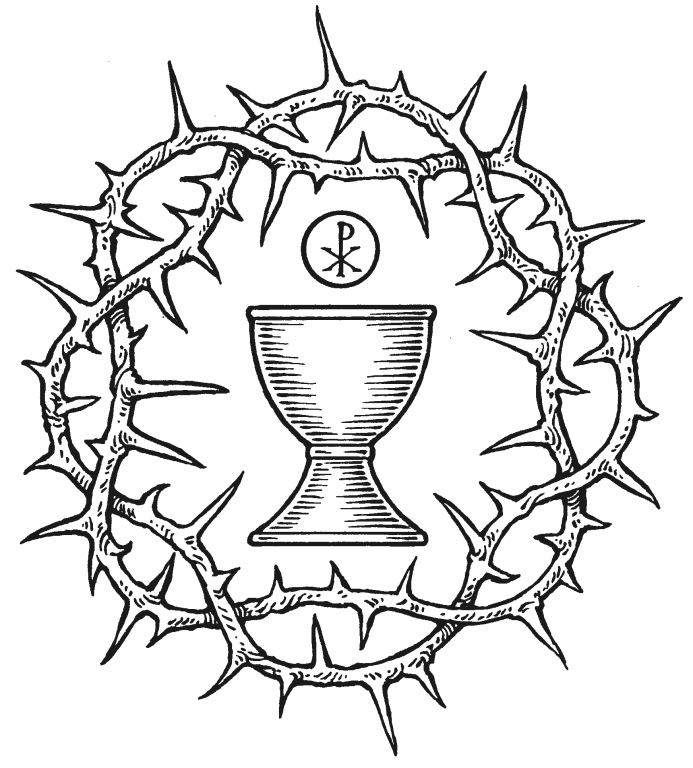
\includegraphics[height=0.4\pageheight]{ofielcatolico/Eucaristia-Coroa.png}
\end{center}
\vfill
\hspace{0pt}
\newpage

\psalm{1}{Le chemin des justes}
\begin{verse}
\versenb{1}Heure\underline{u}x est l’homme \\*
qui n’entre pas au cons\underline{e}il des méchants,~\psalmdagger
qui ne suit pas le chem\underline{i}n des pécheurs,~\psalmstar
ne siège pas avec ce\underline{u}x qui ricanent, \\

\versenb{2}mais se plaît dans la l\underline{o}i du Seigneur \\*
et murmure sa l\underline{o}i jour et nuit! \\

\versenb{3}Il \underline{e}st comme un arbre \\*
plant\underline{é} près d’un ruisseau,~\psalmdagger
qui donne du fr\underline{ui}t en son temps,~\psalmstar
et jamais son feuill\underline{a}ge ne meurt; \\
tout ce qu’il entrepr\underline{e}nd réussira, \\
\versenb{4}tel n’est pas le s\underline{o}rt des méchants. \\*

Mais ils s\underline{o}nt comme la paille \\
balay\underline{é}e par le vent:~\psalmdagger
\versenb{5}au jugement, les méchants ne se l\underline{è}veront pas,~\psalmstar
ni les pécheurs au rassemblem\underline{e}nt des justes. \\
\versenb{6}Le Seigneur connaît le chem\underline{i}n des justes, \\*
mais le chemin des méch\underline{a}nts se perdra. \\
\end{verse}


\psalm{2}{«Tu es mon fils »}
\begin{verse}
\versenb{1}Pourquoi ce tum\underline{u}lte des nations, \\*
ce vain murm\underline{u}re des peuples? \\
\versenb{2}Les rois de la t\underline{e}rre se dressent, \\*
les grands se liguent entre eux
contre le Seigne\underline{u}r et son messie: \\
\versenb{3}«Faisons saut\underline{e}r nos chaînes, \\*
rejet\underline{o}ns ces entraves! » \\

\versenb{4}Celui qui règne dans les cie\underline{u}x s’en amuse, \\*
le Seigneur les to\underline{u}rne en dérision; \\
\versenb{5}puis il leur p\underline{a}rle avec fureur \\*
et sa col\underline{è}re les épouvante: \\
\versenb{6}«Moi, j’ai sacr\underline{é} mon roi \\*
sur Sion, ma s\underline{a}inte mont\underline{a}gne.» \\

\versenb{7}Je proclame le décr\underline{e}t du Seigneur!~\psalmdagger

Il m’a d\underline{i}t: « Tu es mon fils ; \\
moi, aujourd’hu\underline{i}, je t’ai engendré. \\
\versenb{8}Demande, et je te donne en hérit\underline{a}ge les nations, \\*
pour domaine la t\underline{e}rre tout entière. \\
\versenb{9}Tu les détruiras de ton sc\underline{e}ptre de fer, \\*
tu les briseras comme un v\underline{a}se de potier.» \\

\versenb{10}Maintenant, r\underline{o}is, comprenez, \\*
reprenez-vous, j\underline{u}ges de la terre. \\
\versenb{11}Servez le Seigne\underline{u}r avec crainte, \\*
rendez-lui votre homm\underline{a}ge en tremblant. \\
\versenb{12}Qu’il s’irrite et vous \underline{ê}tes perdus: \\*
soudain sa col\underline{è}re éclatera. \\

Heureux qui trouve en lu\underline{i} son refuge! \\
\end{verse}


\psalm{3}{Du Seigneur vient le salut}
\psalmintro{Psaume. De David. Quand il fuyait devant son fils Absalom.}

\begin{verse}
\versenb{2}Seigneur, qu’ils sont nombre\underline{u}x mes adversaires, \\*
nombreux à se lev\underline{e}r contre moi, \\
\versenb{3}nombreux à déclar\underline{e}r à mon sujet: \\*
«Pour lui, pas de sal\underline{u}t auprès de Dieu ! » \\

\versenb{4}Mais toi, Seigne\underline{u}r, mon bouclier, \\*
ma gloire, tu tiens ha\underline{u}te ma tête. \\
\versenb{5}À pleine voix je cr\underline{i}e vers le Seigneur; \\*
il me répond de sa mont\underline{a}gne sainte. \\

\versenb{6}Et moi, je me co\underline{u}che et je dors; \\*
je m’éveille: le Seigne\underline{u}r est mon soutien. \\
\versenb{7}Je ne crains pas ce pe\underline{u}ple nombreux \\*
qui me cerne et s’av\underline{a}nce contre moi. \\

\versenb{8}Lève-t\underline{o}i, Seigneur! \\*
Sauve-m\underline{o}i, mon Dieu! \\
Tous mes ennemis, tu les fr\underline{a}ppes à la mâchoire; \\
les méchants, tu leur br\underline{i}ses les dents. \\

\versenb{9}Du Seigneur vi\underline{e}nt le salut; \\*
vienne ta bénédicti\underline{o}n sur ton peuple! \\
\end{verse}


\psalm{4}{Tu me donnes d’habiter dans la confiance}
\psalmintro{Du maître de chœur. Avec instruments à corde. Psaume.~De~David.}

\begin{verse}
\versenb{2}Quand je cr\underline{i}e, réponds-moi, \\*
Die\underline{u}, ma justice! \\

Toi qui me lib\underline{è}res dans la détresse, \\
pitié pour moi, éco\underline{u}te ma prière! \\

\versenb{3}Fils des hommes, \\*
jusqu’où irez-vous dans l’ins\underline{u}lte à ma gloire,~\psalmstar
l’amour du néant et la co\underline{u}rse au mensonge? \\

\versenb{4}Sachez que le Seigneur a mis à p\underline{a}rt son fidèle, \\*
le Seigneur entend quand je cr\underline{i}e vers lui. \\

\versenb{5}Mais vous, trembl\underline{e}z, ne péchez pas; \\*
réfléchissez dans le secret, f\underline{a}ites silence. \\

\versenb{6}Offrez les offr\underline{a}ndes justes \\*
et faites confi\underline{a}nce au Seigneur. \\

\versenb{7}Beaucoup demandent:
«Qui nous fera v\underline{o}ir le bonheur ? »~\psalmstar
Sur nous, Seigneur, que s’illum\underline{i}ne ton visage! \\

\versenb{8}Tu mets dans mon cœ\underline{u}r plus de joie \\*
que toutes leurs vend\underline{a}nges et leurs moissons. \\

\versenb{9}Dans la paix moi aussi, je me co\underline{u}che et je dors,~\psalmstar
car tu me donnes d’habiter, Seigneur, \\
se\underline{u}l, dans la confiance. \\
\end{verse}


\psalm{5}{Au matin, tu écoutes ma voix}
\psalmintro{Du maître de chœur. Sur les flûtes. Psaume.~De~David.}

\begin{verse}
\versenb{2}Écoute mes par\underline{o}les, Seigneur, \\*
compr\underline{e}nds ma plainte;~\psalmstar
\versenb{3}entends ma v\underline{o}ix qui t’appelle, \\*
ô mon R\underline{o}i et mon Dieu! \\

\versenb{4}Je me tourne vers t\underline{o}i, Seigneur, \\*
au matin, tu éco\underline{u}tes ma voix;~\psalmstar
au matin, je me prép\underline{a}re pour toi \\
et je r\underline{e}ste en éveil. \\

\versenb{5}Tu n’es pas un Die\underline{u} ami du mal, \\*
chez toi, le méch\underline{a}nt n’est pas reçu.~\psalmstar
\versenb{6}Non, l’insens\underline{é} ne tient pas \\*
dev\underline{a}nt ton regard. \\

Tu détestes to\underline{u}s les malfaisants, \\
\versenb{7}tu exterm\underline{i}nes les menteurs;~\psalmstar
l’homme de r\underline{u}se et de sang, \\
le Seigne\underline{u}r le hait. \\

\versenb{8}Pour moi, gr\underline{â}ce à ton amour, \\*
j’acc\underline{è}de à ta maison;~\psalmstar
vers ton temple saint, je me prosterne, \\
sais\underline{i} de crainte. \\

\versenb{9}Seigneur, que ta just\underline{i}ce me conduise;~\psalmstar
des ennem\underline{i}s me guettent: \\
aplanis devant moi ton chemin. \\

\versenb{10}Rien n’est vrai dans leur bouche, \\*
ils sont rempl\underline{i}s de malveillance;~\psalmstar
leur gosier est un sép\underline{u}lcre béant, \\*
et leur l\underline{a}ngue, un piège. \\

\versenb{11}$\[$Dieu, traite-l\underline{e}s en coupables: \\*
qu’ils écho\underline{u}ent dans leurs projets!~\psalmstar
Pour tant de méf\underline{a}its, disperse-les, \\*
p\underline{u}isqu’ils te résistent.$\]$ \\

\versenb{12}Allégresse pour qui s’abr\underline{i}te en toi, \\*
j\underline{o}ie éternelle!~\psalmstar
Tu les protèges, pour t\underline{o}i ils exultent, \\*
ceux qui \underline{a}iment ton nom. \\

\versenb{13}Toi, Seigneur, tu bén\underline{i}s le juste; \\*
du bouclier de ta fave\underline{u}r, tu le couvres. \\
\end{verse}


\psalm{6}{Seigneur, guéris-moi}
\psalmintro{Du maître de chœur. Avec instruments à corde. À l’octave. Psaume.~De~David.}

\begin{verse}
\versenb{2}Seigneur, corrige-m\underline{o}i sans colère, \\*
et reprends-m\underline{o}i sans fureur. \\
\versenb{3}Pitié, Seigne\underline{u}r, je dépéris! \\*
Seigne\underline{u}r, guéris-moi! \\
Car je tremble de to\underline{u}s mes os, \\*
\versenb{4}de toute mon \underline{â}me, je tremble. \\*

Et toi, Seigne\underline{u}r, que fais-tu?~\psalmdagger
\versenb{5}Reviens, Seigne\underline{u}r, délivre-moi, \\*
sauve-moi en rais\underline{o}n de ton amour! \\
\versenb{6}Personne, dans la mort, n’inv\underline{o}que ton nom; \\*
au séjour des morts, qu\underline{i} te rend grâce? \\

\versenb{7}Je m’épuise à f\underline{o}rce de gémir;~\psalmdagger
chaque nuit, je ple\underline{u}re sur mon lit: \\
ma couche est tremp\underline{é}e de mes larmes. \\
\versenb{8}Mes yeux sont rong\underline{é}s de chagrin; \\*
j’ai vieilli parmi t\underline{a}nt d’adversaires! \\

\versenb{9}Loin de moi, vous to\underline{u}s, malfaisants, \\*
car le Seigneur ent\underline{e}nd mes sanglots! \\
\versenb{10}Le Seigneur accu\underline{e}ille ma demande, \\*
le Seigneur ent\underline{e}nd ma prière. \\
\versenb{11}Qu’ils aient honte et qu’ils tremblent, to\underline{u}s mes ennemis, \\*
qu’ils reculent, soud\underline{a}in, couverts de honte! \\
\end{verse}


\psalm{7}{Toi qui scrutes les cœurs et les reins}
\psalmintro{Complainte. De David. Qu’il chanta au Seigneur à propos de Koush~le~Benjaminite.}

\begin{verse}
\versenb{2}Seigneur mon Dieu, tu \underline{e}s mon refuge! \\*
On me poursuit: sauve-m\underline{o}i, délivre-moi ! \\
\versenb{3}Sinon ils vont m’égorg\underline{e}r, tous ces fauves, \\*
me déchirer, sans que pers\underline{o}nne me délivre. \\

\versenb{4}Seigneur mon Dieu, si j’\underline{a}i fait cela, \\*
si j’ai vraiment un cr\underline{i}me sur les mains, \\
\versenb{5}si j’ai causé du t\underline{o}rt à mon allié \\*
en épargn\underline{a}nt son adversaire, \\
\versenb{6}que l’ennemi me poursu\underline{i}ve, qu’il m’atteigne~\psalmstar
(qu’il foule au sol ma vie)
et livre ma gl\underline{o}ire à la poussière. \\

\versenb{7}Dans ta colère, Seigne\underline{u}r, lève-toi,~\psalmdagger
domine mes advers\underline{a}ires en furie, \\
réveille-toi pour me défendre et prononc\underline{e}r ta sentence. \\
\versenb{8}Une assemblée de pe\underline{u}ples t’environne:~\psalmdagger
reprends ta pl\underline{a}ce au-dessus d’elle, \\
\versenb{9}Seigneur qui arb\underline{i}tres les nations. \\*

Juge-moi, Seigne\underline{u}r, sur ma justice: \\
mon innocence p\underline{a}rle pour moi. \\
\versenb{10}Mets fin à la r\underline{a}ge des impies, \\*
afferm\underline{i}s le juste, \\
toi qui scrutes les cœ\underline{u}rs et les reins, \\
Die\underline{u}, le juste. \\

\versenb{11}J’aurai mon boucli\underline{e}r auprès de Dieu, \\*
le sauve\underline{u}r des cœurs droits. \\
\versenb{12}Dieu j\underline{u}ge avec justice; \\*
Dieu menace chaque jour
l’homme qui ne se r\underline{e}prend pas. \\

\versenb{13}Le méchant aff\underline{û}te son épée, \\*
il tend son \underline{a}rc et le tient prêt. \\
\versenb{14}Il se prépare des eng\underline{i}ns de mort; \\*
de ses flèches, il f\underline{a}it des brandons. \\

\versenb{15}Qui conçoit le mal et co\underline{u}ve le crime \\*
enfanter\underline{a} le mensonge. \\
\versenb{16}Qui ouvre une f\underline{o}sse et la creuse \\*
tombera dans le tro\underline{u} qu’il a fait. \\
\versenb{17}Son mauvais coup lui revi\underline{e}nt sur la tête, \\*
sa violence ret\underline{o}mbe sur son crâne. \\

\versenb{18}Je rendrai grâce au Seigne\underline{u}r pour sa justice, \\*
je chanterai le nom du Seigne\underline{u}r, le Très-Haut. \\
\end{verse}


\psalm{8}{Qu’il est grand ton nom!}
\psalmintro{Du maître de chœur. Sur la guittith. Psaume. De David.}

\begin{verse}
\versenb{2}Ô Seigne\underline{u}r, notre Dieu, \\*
qu’il est gr\underline{a}nd, ton nom, \\
par to\underline{u}te la terre! \\

Jusqu’aux cieux, ta splende\underline{u}r est chantée \\
\versenb{3}par la bouche des enf\underline{a}nts, des tout-petits: \\*
rempart que tu opp\underline{o}ses à l’adversaire, \\
où l’ennemi se br\underline{i}se en sa révolte. \\

\versenb{4}À voir ton ciel, ouvr\underline{a}ge de tes doigts, \\*
la lune et les ét\underline{o}iles que tu fixas, \\
\versenb{5}qu’est-ce que l’homme pour que tu p\underline{e}nses à lui, \\*
le fils d’un homme, que tu en pr\underline{e}nnes souci? \\

\versenb{6}Tu l’as voulu un peu m\underline{o}indre qu’un dieu, \\*
le couronnant de gl\underline{o}ire et d’honneur; \\
\versenb{7}tu l’établis sur les œ\underline{u}vres de tes mains, \\*
tu mets toute ch\underline{o}se à ses pieds: \\

\versenb{8}les troupeaux de bœ\underline{u}fs et de brebis, \\*
et même les b\underline{ê}tes sauvages, \\
\versenb{9}les oiseaux du ciel et les poiss\underline{o}ns de la mer, \\*
tout ce qui va son chem\underline{i}n dans les eaux. \\

\versenb{10}Ô Seigne\underline{u}r, notre Dieu, \\*
qu’il est gr\underline{a}nd ton nom \\
par to\underline{u}te la terre! \\
\end{verse}


\psalm{9A}{Tu as jugé avec justice}
\psalmintro{Du maître de chœur. Sur hautbois et harpe. Psaume. De David.}

\begin{verse}
\versenb{2}De tout mon cœur, Seigne\underline{u}r, je rendrai grâce, \\*
je dirai tes innombr\underline{a}bles merveilles; \\
\versenb{3}pour toi, j’exulter\underline{a}i, je danserai, \\*
je fêterai ton n\underline{o}m, Dieu Très-Haut. \\

\versenb{4}Mes ennemis ont batt\underline{u} en retraite, \\*
devant ta face, ils s’écro\underline{u}lent et périssent. \\
\versenb{5}Tu as plaidé mon dr\underline{o}it et ma cause, \\*
tu as siégé, tu as jug\underline{é} avec justice. \\

\versenb{6}Tu menaces les nations, tu fais pér\underline{i}r les méchants, \\*
à tout jamais tu eff\underline{a}ces leur nom. \\
\versenb{7}L’ennemi est achevé, ruin\underline{é} pour toujours, \\*
tu as rasé des villes, leur souven\underline{i}r a péri. \\

\versenb{8}Mais il siège, le Seigne\underline{u}r, à jamais: \\*
pour juger, il afferm\underline{i}t son trône; \\
\versenb{9}il juge le m\underline{o}nde avec justice \\*
et gouverne les pe\underline{u}ples avec droiture. \\

\versenb{10}Qu’il soit la forter\underline{e}sse de l’opprimé, \\*
sa forteresse aux he\underline{u}res d’angoisse: \\
\versenb{11}ils s’appuieront sur toi, ceux qui conn\underline{a}issent ton nom; \\*
jamais tu n’abandonnes, Seigneur, ce\underline{u}x qui te cherchent. \\

\versenb{12}Fêtez le Seigneur qui si\underline{è}ge dans Sion, \\*
annoncez parmi les pe\underline{u}ples ses exploits! \\
\versenb{13}Attentif au sang vers\underline{é}, il se rappelle, \\*
il n’oublie pas le cr\underline{i} des malheureux. \\

\versenb{14}Pitié pour moi, Seigneur, \\*
vois le mal que m’ont f\underline{a}it mes adversaires,~\psalmstar
toi qui m’arraches aux p\underline{o}rtes de la mort; \\
\versenb{15}et je dirai tes innombrables louanges
aux p\underline{o}rtes de Sion,~\psalmstar
je danserai de j\underline{o}ie pour ta victoire. \\

\versenb{16}Ils sont tombés, les païens, dans la f\underline{o}sse qu’ils creusaient; \\*
aux filets qu’ils ont tendus, leurs pi\underline{e}ds se sont pris. \\
\versenb{17}Le Seigneur s’est fait connaître: il a rend\underline{u} le jugement, \\*
il prend les méch\underline{a}nts à leur piège. \\

\versenb{18}Que les méchants reto\underline{u}rnent chez les morts, \\*
toutes les nations qui oubl\underline{i}ent le vrai Dieu! \\
\versenb{19}Mais le pauvre n’est pas oubli\underline{é} pour toujours: \\*
jamais ne périt l’esp\underline{o}ir des malheureux. \\

\versenb{20}Lève-toi, Seigneur: qu’un mortel ne soit p\underline{a}s le plus fort, \\*
que les nations soient jug\underline{é}es devant ta face! \\
\versenb{21}Frappe-les d’épouv\underline{a}nte, Seigneur: \\*
que les nations se reconn\underline{a}issent mortelles! \\
\end{verse}


\psalm{9B}{Tu entends le désir des pauvres}
\begin{verse}
\versenb{1}Pourquoi, Seigne\underline{u}r, es-tu si loin? \\*
Pourquoi te cach\underline{e}r aux jours d’angoisse? \\
\versenb{2}L’impie, dans son orgueil, poursu\underline{i}t les malheureux: \\*
ils se font prendre aux r\underline{u}ses qu’il invente. \\

\versenb{3}L’impie se glorifie du dés\underline{i}r de son âme, \\*
l’arrogant blasphème, il br\underline{a}ve le Seigneur; \\
\versenb{4}plein de suffisance, l’imp\underline{i}e ne cherche plus: \\*
«Dieu n’est rien », voil\underline{à} toute sa ruse. \\

\versenb{5}À tout moment, ce qu’il f\underline{a}it réussit;~\psalmdagger
tes sentences le dom\underline{i}nent de très haut.~\psalmstar
(Tous ses advers\underline{a}ires, il les méprise.) \\
\versenb{6}Il s’est dit: « Rien ne pe\underline{u}t m’ébranler, \\*
je suis pour longtemps à l’abr\underline{i} du malheur.» \\

\versenb{7}Sa bouche qui maudit n’est que fra\underline{u}de et violence, \\*
sa langue, mens\underline{o}nge et blessure. \\
\versenb{8}Il se tient à l’aff\underline{û}t près des villages, \\*
il se cache pour tu\underline{e}r l’innocent. \\

Des yeux, il ép\underline{i}e le faible, \\
\versenb{9}il se cache à l’affût, comme un li\underline{o}n dans son fourré; \\*
il se tient à l’affût pour surpr\underline{e}ndre le pauvre, \\
il attire le pauvre, il le pr\underline{e}nd dans son filet. \\

\versenb{10}Il se b\underline{a}isse, il se tapit; \\*
de tout son poids, il t\underline{o}mbe sur le faible. \\
\versenb{11}Il dit en lui-même: « Die\underline{u} oublie ! \\*
il couvre sa face, jam\underline{a}is il ne verra! » \\

\versenb{12}Lève-toi, Seigneur! Die\underline{u}, étends la main ! \\*
N’oublie p\underline{a}s le pauvre! \\
\versenb{13}Pourquoi l’impie brave-t-\underline{i}l le Seigneur \\*
en lui disant: « Viendras-t\underline{u} me chercher ? » \\

\versenb{14}Mais tu as vu: tu regardes le m\underline{a}l et la souffrance, \\*
tu les pr\underline{e}nds dans ta main; \\
sur toi rep\underline{o}se le faible, \\
c’est toi qui viens en \underline{a}ide à l’orphelin. \\

\versenb{15}Brise le bras de l’imp\underline{i}e, du méchant; \\*
alors tu chercheras son impiét\underline{é} sans la trouver. \\
\versenb{16}À tout jamais, le Seigne\underline{u}r est roi: \\*
les païens ont pér\underline{i} sur sa terre. \\

\versenb{17}Tu entends, Seigneur, le dés\underline{i}r des pauvres, \\*
tu rassures leur cœ\underline{u}r, tu les écoutes. \\
\versenb{18}Que justice soit rendue à l’orphelin, \\*
qu’il n’y ait pl\underline{u}s d’opprimé,~\psalmstar
et que tremble le mortel, n\underline{é} de la terre! \\
\end{verse}


\psalm{10}{Il garde les yeux ouverts sur le monde}
\psalmintro{Du maître de chœur. De David.}

\begin{verse}
Auprès du Seigne\underline{u}r j’ai mon refuge.\psalmdagger
Comment pouvez-vo\underline{u}s me dire: \\
oiseaux, fuy\underline{e}z à la montagne! \\

\versenb{2}Voici que les méch\underline{a}nts tendent l’arc:~\psalmdagger
ils ajustent leur fl\underline{è}che à la corde \\
pour viser dans l’ombre l’h\underline{o}mme au cœur droit. \\

\versenb{3}Quand sont ruin\underline{é}es les fondations, \\*
que peut f\underline{a}ire le juste? \\

\versenb{4}Mais le Seigneur, dans son t\underline{e}mple saint,~\psalmdagger
le Seigneur, dans les cie\underline{u}x où il trône, \\
garde les yeux ouv\underline{e}rts sur le monde. \\

Il voit, il scr\underline{u}te les hommes;~\psalmdagger
\versenb{5}le Seigneur a scruté le j\underline{u}ste et le méchant: \\*
l’ami de la viol\underline{e}nce, il le hait. \\

\versenb{6}Il fera pleuvoir ses fléa\underline{u}x sur les méchants,~\psalmdagger
feu et soufre et v\underline{e}nt de tempête; \\
c’est la coupe qu’ils aur\underline{o}nt en partage. \\

\versenb{7}Vraiment, le Seigne\underline{u}r est juste;~\psalmdagger
il aime to\underline{u}te justice: \\
les hommes droits le verr\underline{o}nt face à face. \\
\end{verse}


\psalm{11}{Toi, tu tiens parole}
\psalmintro{Du maître de chœur. À l’octave. Psaume. De David.}

\begin{verse}
\versenb{2}Seigneur, au secours! Il n’y a pl\underline{u}s de fidèle ! \\*
La loyauté a dispar\underline{u} chez les hommes. \\
\versenb{3}Entre eux la par\underline{o}le est mensonge, \\*
cœur double, l\underline{è}vres menteuses. \\

\versenb{4}Que le Seigneur supprime ces l\underline{è}vres menteuses, \\*
cette langue qui p\underline{a}rle insolemment, \\
\versenb{5}ceux-là qui disent: « Arm\underline{o}ns notre langue ! \\*
À nous la parole! Qui ser\underline{a} notre maître ? » \\

\versenb{6}–« Pour le pauvre qui gémit, \\*
le malheure\underline{u}x que l’on dépouille,~\psalmdagger
maintenant je me lève, d\underline{i}t le Seigneur;~\psalmstar
à celui qu’on méprise, je p\underline{o}rte secours.» \\

\versenb{7}Les paroles du Seigneur sont des par\underline{o}les pures, \\*
argent passé au feu, affin\underline{é} sept fois. \\
\versenb{8}Toi, Seigne\underline{u}r, tu tiens parole, \\*
tu nous gardes pour toujo\underline{u}rs de cette engeance. \\

\versenb{9}De tous côtés, s’ag\underline{i}tent les impies: \\*
la corruption g\underline{a}gne chez les hommes. \\
\end{verse}


\psalm{12}{Vas-tu m’oublier?}
\psalmintro{Du maître de chœur. Psaume. De David.}

\begin{verse}
\versenb{2}Combien de temps, Seigneur, vas-t\underline{u} m’oublier, \\*
combien de temps, me cach\underline{e}r ton visage? \\
\versenb{3}Combien de temps aurai-je l’âme en peine
et le cœur attrist\underline{é} chaque jour?~\psalmstar
Combien de temps mon ennemi sera-t-\underline{i}l le plus fort? \\

\versenb{4}Regarde, réponds-moi, Seigne\underline{u}r mon Dieu!~\psalmstar
Donne la lumière à mes yeux, \\
garde-moi du somm\underline{e}il de la mort; \\
\versenb{5}que l’adversaire ne crie p\underline{a}s: « Victoire ! », \\*
que l’ennemi n’ait pas la j\underline{o}ie de ma défaite! \\

\versenb{6}Moi, je prends appu\underline{i} sur ton amour;~\psalmdagger
que mon cœur ait la j\underline{o}ie de ton salut! \\
Je chanterai le Seigneur pour le bi\underline{e}n qu’il m’a fait. \\
\end{verse}


\psalm{13}{Pas un homme de bien!}
\psalmintro{Du maître de chœur. De David.}

\begin{verse}
Dans son cœur le fo\underline{u} déclare: \\
«P\underline{a}s de Dieu ! »~\psalmstar
Tout est corromp\underline{u}, abominable, \\
pas un h\underline{o}mme de bien! \\

\versenb{2}Des cieux, le Seigne\underline{u}r se penche \\*
v\underline{e}rs les fils d’Adam~\psalmstar
pour voir s’il en est \underline{u}n de sensé, \\
\underline{u}n qui cherche Dieu. \\

\versenb{3}Tous, ils s\underline{o}nt dévoyés; \\*
tous ens\underline{e}mble, pervertis:~\psalmstar
pas un h\underline{o}mme de bien, \\
pas m\underline{ê}me un seul! \\

\versenb{4}N’ont-ils d\underline{o}nc pas compris, \\*
ces g\underline{e}ns qui font le mal?~\psalmdagger
Quand ils mangent leur pain, \\
ils m\underline{a}ngent mon peuple.~\psalmstar
Jamais ils n’inv\underline{o}quent le Seigneur. \\

\versenb{5}Et voilà qu’ils se sont m\underline{i}s à trembler, \\*
car Dieu accomp\underline{a}gne les justes.~\psalmstar
\versenb{6}Vous riez des proj\underline{e}ts du malheureux, \\*
mais le Seigne\underline{u}r est son refuge. \\

\versenb{7}Qui fera ven\underline{i}r de Sion \\*
la délivr\underline{a}nce d’Israël?~\psalmdagger
Quand le Seigneur ramènera les déport\underline{é}s de son peuple,~\psalmstar
quelle fête en Jacob, en Isra\underline{ë}l, quelle joie! \\
\end{verse}


\psalm{14}{Qui séjournera sous ta tente?}
\psalmintro{Psaume. De David.}

\begin{verse}
Seigneur, qui séjourner\underline{a} sous ta tente? \\
Qui habitera ta s\underline{a}inte montagne? \\

\versenb{2}Celui qui se condu\underline{i}t parfaitement,~\psalmdagger
qui ag\underline{i}t avec justice \\
et dit la vérit\underline{é} selon son cœur. \\

\versenb{3}Il met un fr\underline{e}in à sa langue,~\psalmdagger
ne fait pas de t\underline{o}rt à son frère \\
et n’outrage p\underline{a}s son prochain. \\

\versenb{4}À ses yeux, le réprouv\underline{é} est méprisable \\*
mais il honore les fid\underline{è}les du Seigneur. \\

S’il a jur\underline{é} à ses dépens, \\
il ne reprend p\underline{a}s sa parole. \\

\versenb{5}Il prête son arg\underline{e}nt sans intérêt,~\psalmdagger
n’accepte rien qui nu\underline{i}se à l’innocent. \\
Qui fait ainsi deme\underline{u}re inébranlable. \\
\end{verse}


\psalm{15}{Seigneur, mon partage}
\psalmintro{Miktâm. De David.}

\begin{verse}
Garde-m\underline{o}i, mon Dieu: \\
j’ai fait de t\underline{o}i mon refuge. \\
\versenb{2}J’ai dit au Seigneur: « Tu \underline{e}s mon Dieu ! \\*
Je n’ai pas d’autre bonhe\underline{u}r que toi.» \\

\versenb{3}Toutes les idoles du pays, \\*
ces die\underline{u}x que j’aimais,~\psalmdagger
ne cessent d’ét\underline{e}ndre leurs ravages,~\psalmstar
et l’on se r\underline{u}e à leur suite. \\
\versenb{4}Je n’irai pas leur offrir le s\underline{a}ng des sacrifices;~\psalmstar
leur nom ne viendra p\underline{a}s sur mes lèvres! \\

\versenb{5}Seigneur, mon part\underline{a}ge et ma coupe: \\*
de toi dép\underline{e}nd mon sort. \\
\versenb{6}La part qui me revi\underline{e}nt fait mes délices; \\*
j’ai même le plus b\underline{e}l héritage! \\

\versenb{7}Je bénis le Seigne\underline{u}r qui me conseille: \\*
même la nuit mon cœ\underline{u}r m’avertit. \\
\versenb{8}Je garde le Seigneur devant m\underline{o}i sans relâche; \\*
il est à ma droite: je su\underline{i}s inébranlable. \\

\versenb{9}Mon cœur exulte, mon \underline{â}me est en fête, \\*
ma chair elle-même rep\underline{o}se en confiance: \\
\versenb{10}tu ne peux m’abandonn\underline{e}r à la mort \\*
ni laisser ton ami v\underline{o}ir la corruption. \\

\versenb{11}Tu m’apprends le chem\underline{i}n de la vie:~\psalmdagger
devant ta face, débordem\underline{e}nt de joie! \\
À ta droite, éternit\underline{é} de délices! \\
\end{verse}


\psalm{16}{Garde-moi}
\psalmintro{Prière. De David.}

\begin{verse}
Seigneur, éco\underline{u}te la justice!~\psalmdagger
Entends ma plainte, accu\underline{e}ille ma prière: \\
mes lèvres ne m\underline{e}ntent pas. \\

\versenb{2}De ta face, me viendr\underline{a} la sentence: \\*
tes yeux verr\underline{o}nt où est le droit. \\

\versenb{3}Tu sondes mon cœur, tu me vis\underline{i}tes la nuit,~\psalmdagger
tu m’éprouves, sans ri\underline{e}n trouver; \\
mes pensées n’ont pas franch\underline{i} mes lèvres. \\

\versenb{4}Pour me conduire sel\underline{o}n ta parole, \\*
j’ai gardé le chem\underline{i}n prescrit; \\
\versenb{5}j’ai tenu mes p\underline{a}s sur tes traces: \\*
jamais mon pi\underline{e}d n’a trébuché. \\

\versenb{6}Je t’appelle, toi, le Die\underline{u} qui répond: \\*
écoute-moi, ent\underline{e}nds ce que je dis. \\

\versenb{7}Montre les merv\underline{e}illes de ta grâce,~\psalmstar
toi qui libères de l’agresseur
ceux qui se réfug\underline{i}ent sous ta droite. \\

\versenb{8}Garde-moi comme la prun\underline{e}lle de l’œil; \\*
à l’ombre de tes \underline{a}iles, cache-moi, \\
\versenb{9}loin des méch\underline{a}nts qui m’ont ruiné, \\*
des ennemis mort\underline{e}ls qui m’entourent. \\

\versenb{10}Ils s’enferment d\underline{a}ns leur suffisance; \\*
l’arrogance à la bo\underline{u}che, ils parlent. \\

\versenb{11}Ils sont sur mes pas: mainten\underline{a}nt ils me cernent, \\*
l’œil sur moi, pour me jet\underline{e}r à terre, \\
\versenb{12}comme des lions pr\underline{ê}ts au carnage, \\*
de jeunes fauves tap\underline{i}s en embuscade. \\

\versenb{13}Lève-toi, Seigneur, affronte-l\underline{e}s, renverse-les; \\*
par ton épée, libère-m\underline{o}i des méchants. \\

\versenb{14}Que ta main, Seigneur, les excl\underline{u}e d’entre les hommes,~\psalmstar
hors de l’humanité, hors de ce monde:
tel soit le s\underline{o}rt de leur vie! \\

Réserve-leur de qu\underline{o}i les rassasier:~\psalmdagger
que leurs fils en s\underline{o}ient saturés, \\
qu’il en reste enc\underline{o}re pour leurs enfants! \\

\versenb{15}Et moi, par ta justice, je verr\underline{a}i ta face: \\*
au réveil, je me rassasier\underline{a}i de ton visage. \\
\end{verse}


\psalm{17}{Il m’a libéré, car il m’aime}
\psalmintro{Du maître de chœur. Du serviteur du Seigneur, de David, qui adressa au Seigneur les paroles de ce cantique, au jour où le Seigneur le délivra de la main de tous ses ennemis et de la main de Saül. Il dit:}

\begin{verse}
\versenb{2}Je t’aime, Seigne\underline{u}r, ma force: \\*
Seigneur, mon r\underline{o}c, ma forteresse, \\
\versenb{3}Dieu mon libérateur, le roch\underline{e}r qui m’abrite, \\*
mon bouclier, mon fort, mon \underline{a}rme de victoire! \\

\versenb{4}Lou\underline{a}nge à Dieu!~\psalmdagger
Quand je fais app\underline{e}l au Seigneur,~\psalmstar
je suis sauvé de to\underline{u}s mes ennemis. \\

\versenb{5}Les liens de la m\underline{o}rt m’entouraient, \\*
le torrent fat\underline{a}l m’épouvantait; \\
\versenb{6}des liens inferna\underline{u}x m’étreignaient: \\*
j’étais pris aux pi\underline{è}ges de la mort. \\

\versenb{7}Dans mon angoisse, j’appel\underline{a}i le Seigneur; \\*
vers mon Dieu, je lanç\underline{a}i un cri; \\
de son temple il ent\underline{e}nd ma voix: \\
mon cri parvi\underline{e}nt à ses oreilles. \\

\versenb{8}La terre tit\underline{u}be et tremble,~\psalmdagger
les assises des mont\underline{a}gnes frémissent, \\
secouées par l’explosi\underline{o}n de sa colère. \\

\versenb{9}Une fumée s\underline{o}rt de ses narines,~\psalmdagger
de sa bouche, un fe\underline{u} qui dévore, \\
une gerbe de charb\underline{o}ns embrasés. \\

\versenb{10}Il incline les cie\underline{u}x et descend, \\*
une sombre nu\underline{é}e sous ses pieds: \\
\versenb{11}d’un Kéroub, il f\underline{a}it sa monture, \\*
il vole sur les \underline{a}iles du vent. \\

\versenb{12}Il se cache au s\underline{e}in des ténèbres~\psalmdagger
et dans leurs repl\underline{i}s se dérobe: \\
nuées sur nuées, tén\underline{è}bres diluviennes. \\

\versenb{13}Une lue\underline{u}r le précède,~\psalmdagger
ses nu\underline{a}ges déferlent: \\
grêle et g\underline{e}rbes de feu. \\

\versenb{14}Tonnerre du Seigne\underline{u}r dans le ciel,~\psalmstar
le Très-Haut fait entendre sa voix:
grêle et g\underline{e}rbes de feu. \\
\versenb{15}De tous côtés, il t\underline{i}re des flèches, \\*
il décoche des éclairs, il rép\underline{a}nd la terreur. \\

\versenb{16}Alors le fond des m\underline{e}rs se découvrit, \\*
les assises du m\underline{o}nde apparurent, \\
sous ta voix menaç\underline{a}nte, Seigneur, \\
au souffle qu’exhal\underline{a}it ta colère. \\

\versenb{17}Des hauteurs il tend la m\underline{a}in pour me saisir, \\*
il me retire du go\underline{u}ffre des eaux; \\
\versenb{18}il me délivre d’un puiss\underline{a}nt ennemi, \\*
d’adversaires plus f\underline{o}rts que moi. \\

\versenb{19}Au jour de ma déf\underline{a}ite ils m’attendaient, \\*
mais j’avais le Seigne\underline{u}r pour appui. \\
\versenb{20}Et lui m’a dégag\underline{é}, mis au large, \\*
il m’a libér\underline{é}, car il m’aime. \\

\versenb{21}Le Seigneur me traite sel\underline{o}n ma justice, \\*
il me donne le sal\underline{a}ire des mains pures, \\
\versenb{22}car j’ai gardé les chem\underline{i}ns du Seigneur, \\*
jamais je n’ai trah\underline{i} mon Dieu. \\

\versenb{23}Ses ordres sont to\underline{u}s devant moi, \\*
jamais je ne m’éc\underline{a}rte de ses lois. \\
\versenb{24}Je suis sans repr\underline{o}che envers lui, \\*
je me garde l\underline{o}in du péché. \\
\versenb{25}Le Seigneur me donne sel\underline{o}n ma justice, \\*
selon la pureté des m\underline{a}ins que je lui tends. \\

\versenb{26}Tu es fidèle envers l’h\underline{o}mme fidèle, \\*
sans reproche avec l’h\underline{o}mme sans reproche; \\
\versenb{27}envers qui est loy\underline{a}l, tu es loyal, \\*
tu ruses av\underline{e}c le pervers. \\

\versenb{28}Tu sauves le pe\underline{u}ple des humbles; \\*
les regards haut\underline{a}ins, tu les rabaisses. \\
\versenb{29}Tu es la lumi\underline{è}re de ma lampe, \\*
Seigneur mon Dieu, tu écl\underline{a}ires ma nuit. \\
\versenb{30}Grâce à toi, je sa\underline{u}te le fossé, \\*
grâce à mon Dieu, je franch\underline{i}s la muraille. \\

\versenb{31}Ce Dieu a des chem\underline{i}ns sans reproche,~\psalmdagger
la parole du Seigne\underline{u}r est sans alliage, \\
il est un bouclier pour qui s’abr\underline{i}te en lui. \\

\versenb{32}Qui est Dieu, horm\underline{i}s le Seigneur? \\*
le Rocher, sin\underline{o}n notre Dieu? \\
\versenb{33}C’est le Dieu qui m’empl\underline{i}t de vaillance \\*
et m’indique un chem\underline{i}n sans reproche. \\

\versenb{34}Il me donne l’agilit\underline{é} du chamois, \\*
il me tient debo\underline{u}t sur les hauteurs, \\
\versenb{35}il exerce mes m\underline{a}ins à combattre \\*
et mon bras, à t\underline{e}ndre l’arc. \\

\versenb{36}Par ton bouclier tu m’ass\underline{u}res la victoire, \\*
ta droite me soutient, ta pati\underline{e}nce m’élève. \\
\versenb{37}C’est toi qui all\underline{o}nges ma foulée \\*
sans que faibl\underline{i}ssent mes chevilles. \\

\versenb{38}Je poursuis mes ennem\underline{i}s, je les rejoins, \\*
je ne reviens qu’apr\underline{è}s leur défaite; \\
\versenb{39}je les abats: ils ne pourr\underline{o}nt se relever ; \\*
ils tombent: les voil\underline{à} sous mes pieds. \\

\versenb{40}Pour le combat tu m’empl\underline{i}s de vaillance; \\*
devant moi tu fais pli\underline{e}r mes agresseurs. \\
\versenb{41}Tu me livres des ennem\underline{i}s en déroute; \\*
j’anéant\underline{i}s mes adversaires. \\

\versenb{42}Ils appellent? p\underline{a}s de sauveur ! \\*
le Seigneur? p\underline{a}s de réponse ! \\
\versenb{43}J’en fais de la poussi\underline{è}re pour le vent, \\*
de la boue qu’on enl\underline{è}ve des rues. \\

\versenb{44}Tu me libères des quer\underline{e}lles du peuple, \\*
tu me places à la t\underline{ê}te des nations. \\
Un peuple d’inconn\underline{u}s m’est asservi: \\
\versenb{45}au premier m\underline{o}t, ils m’obéissent. \\*

Ces fils d’étrang\underline{e}rs se soumettent;~\psalmdagger
\versenb{46}ces fils d’étrang\underline{e}rs capitulent: \\*
en tremblant ils qu\underline{i}ttent leurs bastions. \\

\versenb{47}Vive le Seigneur! Bén\underline{i} soit mon Rocher ! \\*
Qu’il triomphe, le Die\underline{u} de ma victoire, \\
\versenb{48}ce Dieu qui m’acc\underline{o}rde la revanche, \\*
qui soumet à mon pouv\underline{o}ir les nations! \\

\versenb{49}Tu me délivres de to\underline{u}s mes ennemis,~\psalmdagger
tu me fais triomph\underline{e}r de l’agresseur, \\
tu m’arraches à la viol\underline{e}nce de l’homme. \\

\versenb{50}Aussi, je te rendrai gr\underline{â}ce parmi les peuples, \\*
Seigneur, je fêter\underline{a}i ton nom. \\
\versenb{51}Il donne à son roi de gr\underline{a}ndes victoires,~\psalmstar
il se montre fidèle à son messie, \\
à David et sa descend\underline{a}nce, pour toujours. \\
\end{verse}


\psalm{18A}{Les cieux proclament la gloire de Dieu}
\psalmintro{Du maître de chœur. Psaume. De David.}

\begin{verse}
\versenb{2}Les cieux proclament la gl\underline{o}ire de Dieu, \\*
le firmament raconte l’ouvr\underline{a}ge de ses mains. \\
\versenb{3}Le jour au jour en l\underline{i}vre le récit \\*
et la nuit à la nuit en d\underline{o}nne connaissance. \\

\versenb{4}Pas de par\underline{o}les dans ce récit, \\*
pas de v\underline{o}ix qui s’entende; \\
\versenb{5}mais sur toute la terre en par\underline{a}ît le message \\*
et la nouvelle, aux lim\underline{i}tes du monde. \\

Là, se trouve la deme\underline{u}re du soleil:~\psalmdagger
\versenb{6}tel un époux, il par\underline{a}ît hors de sa tente, \\*
il s’élance en conquér\underline{a}nt joyeux. \\

\versenb{7}Il paraît où comm\underline{e}nce le ciel,~\psalmdagger
il s’en va jusqu’où le ci\underline{e}l s’achève: \\
rien n’éch\underline{a}ppe à son ardeur. \\
\end{verse}


\psalm{18B}{La loi qui clarifie le regard}
\begin{verse}
\versenb{8}La loi du Seigne\underline{u}r est parfaite, \\*
qui red\underline{o}nne vie;~\psalmstar
la charte du Seigne\underline{u}r est sûre, \\
qui rend s\underline{a}ges les simples. \\

\versenb{9}Les préceptes du Seigne\underline{u}r sont droits, \\*
ils réjou\underline{i}ssent le cœur;~\psalmstar
le commandement du Seigne\underline{u}r est limpide, \\
il clarif\underline{i}e le regard. \\

\versenb{10}La crainte qu’il insp\underline{i}re est pure, \\*
elle est l\underline{à} pour toujours;~\psalmstar
les décisions du Seigne\underline{u}r sont justes \\
et vraim\underline{e}nt équitables: \\

\versenb{11}plus désir\underline{a}bles que l’or, \\*
qu’une m\underline{a}sse d’or fin,~\psalmstar
plus savoure\underline{u}ses que le miel \\*
qui co\underline{u}le des rayons. \\

\versenb{12}Aussi ton serviteur en \underline{e}st illuminé;~\psalmdagger
à les garder, il tro\underline{u}ve son profit.~\psalmstar
\versenb{13}Qui peut discern\underline{e}r ses erreurs? \\*
Purifie-moi de c\underline{e}lles qui m’échappent. \\

\versenb{14}Préserve aussi ton servite\underline{u}r de l’orgueil: \\*
qu’il n’ait sur m\underline{o}i aucune emprise.~\psalmstar
Alors je ser\underline{a}i sans reproche, \\*
p\underline{u}r d’un grand péché. \\

\versenb{15}Accueille les par\underline{o}les de ma bouche, \\*
le murm\underline{u}re de mon cœur;~\psalmstar
qu’ils parvi\underline{e}nnent devant toi, \\*
Seigneur, mon roch\underline{e}r, mon défenseur! \\
\end{verse}


\psalm{19}{Il donne la victoire à son messie}
\psalmintro{Du maître de chœur. Psaume. De David.}

\begin{verse}
\versenb{2}Que le Seigneur te réponde au jo\underline{u}r de détresse, \\*
que le nom du Dieu de Jac\underline{o}b te défende. \\
\versenb{3}Du sanctuaire, qu’il t’env\underline{o}ie le secours, \\*
qu’il te soutienne des haute\underline{u}rs de Sion. \\

\versenb{4}Qu’il se rappelle to\underline{u}tes tes offrandes; \\*
ton holocauste, qu’il le tro\underline{u}ve savoureux. \\
\versenb{5}Qu’il te donne à la mes\underline{u}re de ton cœur, \\*
qu’il accomplisse to\underline{u}s tes projets. \\

\versenb{6}Nous acclamerons ta victoire
en arborant le n\underline{o}m de notre Dieu.~\psalmstar
Le Seigneur accomplira
to\underline{u}tes tes demandes. \\

\versenb{7}Maintenant, je le sais:
le Seigneur donne la vict\underline{o}ire à son messie;~\psalmstar
du sanctuaire des cieux, il lui répond
par les exploits de sa m\underline{a}in victorieuse. \\

\versenb{8}Aux uns, les chars; aux a\underline{u}tres, les chevaux ; \\*
à nous, le nom de notre Die\underline{u}: le Seigneur. \\
\versenb{9}Eux, ils pl\underline{i}ent et s’effondrent; \\*
nous, debo\underline{u}t, nous résistons. \\

\versenb{10}Seigneur, donne au r\underline{o}i la victoire! \\*
Réponds-nous au jo\underline{u}r de notre appel. \\
\end{verse}


\psalm{20}{Dresse-toi dans ta force}
\psalmintro{Du maître de chœur. Psaume. De David.}

\begin{verse}
\versenb{2}Seigneur, le roi se réjou\underline{i}t de ta force; \\*
quelle allégresse lui d\underline{o}nne ta victoire! \\
\versenb{3}Tu as répondu au dés\underline{i}r de son cœur, \\*
tu n’as pas rejeté le souh\underline{a}it de ses lèvres. \\

\versenb{4}Tu lui destines bénédicti\underline{o}ns et bienfaits, \\*
tu mets sur sa tête une cour\underline{o}nne d’or. \\
\versenb{5}La vie qu’il t’a demand\underline{é}e, tu la lui donnes, \\*
de longs jours, des ann\underline{é}es sans fin. \\

\versenb{6}Par ta victoire, grand\underline{i}t son éclat: \\*
tu le revêts de splende\underline{u}r et de gloire. \\
\versenb{7}Tu mets en lui ta bénédicti\underline{o}n pour toujours: \\*
ta présence l’empl\underline{i}t de joie! \\

\versenb{8}Oui, le roi s’appu\underline{i}e sur le Seigneur: \\*
la grâce du Très-Haut le r\underline{e}nd inébranlable. \\
\versenb{9}$\[$Ta main trouver\underline{a} tes ennemis, \\*
ta droite trouver\underline{a} tes adversaires. \\

\versenb{10}Tu parais, tu en f\underline{a}is un brasier: \\*
la colère du Seigneur les consume, \\
un fe\underline{u} les dévore. \\
\versenb{11}Tu aboliras leur lign\underline{é}e sur la terre \\*
et leur descendance parm\underline{i} les hommes. \\

\versenb{12}S’ils trament le mal contre toi, \\*
s’ils prép\underline{a}rent un complot,~\psalmstar
ils ir\underline{o}nt à l’échec. \\
\versenb{13}Oui, tu les renv\underline{e}rses et les terrasses; \\*
ton arc les v\underline{i}se en plein cœur.$\]$ \\

\versenb{14}Dresse-toi, Seigne\underline{u}r, dans ta force: \\*
nous fêterons, nous chanter\underline{o}ns ta vaillance. \\
\end{verse}


\psalm{21}{Mon Dieu, pourquoi m’as-tu abandonné?}
\psalmintro{Du maître de chœur. Sur l’air de «La biche de l’aurore ». Psaume.~De~David.}

\begin{verse}
\versenb{2}Mon Die\underline{u}, mon Dieu, \\*
pourquoi m’as-t\underline{u} abandonné?~\psalmstar
Le sal\underline{u}t est loin de moi, \\
loin des m\underline{o}ts que je rugis. \\

\versenb{3}Mon Dieu, j’app\underline{e}lle tout le jour, \\*
et tu ne r\underline{é}ponds pas;~\psalmstar
m\underline{ê}me la nuit, \\
je n’ai p\underline{a}s de repos. \\

\versenb{4}Toi, pourt\underline{a}nt, tu es saint, \\*
toi qui habites les h\underline{y}mnes d’Israël! \\
\versenb{5}C’est en toi que nos p\underline{è}res espéraient, \\*
ils espéraient et tu les d\underline{é}livrais. \\
\versenb{6}Quand ils criaient vers t\underline{o}i, ils échappaient; \\*
en toi ils espéraient et n’étaient p\underline{a}s déçus. \\

\versenb{7}Et moi, je suis un v\underline{e}r, pas un homme, \\*
raillé par les gens, rejet\underline{é} par le peuple. \\
\versenb{8}Tous ceux qui me v\underline{o}ient me bafouent, \\*
ils ricanent et h\underline{o}chent la tête: \\
\versenb{9}«Il comptait sur le Seigne\underline{u}r : qu’il le délivre ! \\*
Qu’il le sauve, puisqu’il \underline{e}st son ami! » \\

\versenb{10}C’est toi qui m’as tiré du v\underline{e}ntre de ma mère, \\*
qui m’a mis en sûret\underline{é} entre ses bras. \\
\versenb{11}À toi je fus confi\underline{é} dès ma naissance; \\*
dès le ventre de ma m\underline{è}re, tu es mon Dieu. \\

\versenb{12}Ne sois pas loin: l’ang\underline{o}isse est proche, \\*
je n’ai pers\underline{o}nne pour m’aider. \\
\versenb{13}Des fauves nombre\underline{u}x me cernent, \\*
des taureaux de Bash\underline{a}ne m’encerclent. \\
\versenb{14}Des lions qui déch\underline{i}rent et rugissent \\*
ouvrent leur gue\underline{u}le contre moi. \\

\versenb{15}Je suis comme l’ea\underline{u} qui se répand, \\*
tous mes m\underline{e}mbres se disloquent. \\
Mon cœur est c\underline{o}mme la cire, \\
il fond au milie\underline{u} de mes entrailles. \\
\versenb{16}Ma vigueur a séch\underline{é} comme l’argile, \\*
ma langue c\underline{o}lle à mon palais. \\

Tu me mènes à la poussi\underline{è}re de la mort.~\psalmdagger

\versenb{17}Oui, des chi\underline{e}ns me cernent, \\*
une bande de vauri\underline{e}ns m’entoure. \\
Ils me percent les m\underline{a}ins et les pieds; \\
\versenb{18}je peux compt\underline{e}r tous mes os. \\*

Ces gens me v\underline{o}ient, ils me regardent.~\psalmdagger
\versenb{19}Ils partagent entre e\underline{u}x mes habits \\*
et tirent au s\underline{o}rt mon vêtement. \\

\versenb{20}Mais toi, Seigne\underline{u}r, ne sois pas loin: \\*
ô ma force, viens v\underline{i}te à mon aide! \\
\versenb{21}Préserve ma v\underline{i}e de l’épée, \\*
arrache-moi aux gr\underline{i}ffes du chien; \\
\versenb{22}sauve-moi de la gue\underline{u}le du lion \\*
et de la c\underline{o}rne des buffles. \\

Tu m’\underline{a}s répondu!~\psalmdagger
\versenb{23}Et je proclame ton n\underline{o}m devant mes frères, \\*
je te loue en pl\underline{e}ine assemblée. \\

\versenb{24}Vous qui le craignez, lou\underline{e}z le Seigneur,~\psalmdagger
glorifiez-le, vous tous, descend\underline{a}nts de Jacob, \\
vous tous, redoutez-le, descend\underline{a}nts d’Israël. \\

\versenb{25}Car il n’a p\underline{a}s rejeté, \\*
il n’a pas réprouvé le malheure\underline{u}x dans sa misère; \\
il ne s’est pas voilé la f\underline{a}ce devant lui, \\
mais il ent\underline{e}nd sa plainte. \\

\versenb{26}Tu seras ma louange dans la gr\underline{a}nde assemblée; \\*
devant ceux qui te craignent, je tiendr\underline{a}i mes promesses. \\
\versenb{27}Les pauvres mangeront: ils ser\underline{o}nt rassasiés ; \\*
ils loueront le Seigneur, ceux qui le cherchent:
«À vous, toujours, la v\underline{i}e et la joie ! » \\

\versenb{28}La terre entière se souviendra
et reviendr\underline{a} vers le Seigneur, \\
chaque famille de nations se prosterner\underline{a} devant lui: \\
\versenb{29}«Oui, au Seigne\underline{u}r la royauté, \\*
le pouv\underline{o}ir sur les nations! » \\

\versenb{30}Tous ceux qui festoy\underline{a}ient s’inclinent; \\*
promis à la mort, ils pl\underline{i}ent en sa présence. \\

\versenb{31}Et moi, je vis pour lui: ma descend\underline{a}nce le servira ; \\*
on annoncera le Seigneur aux générati\underline{o}ns à venir. \\
\versenb{32}On proclamera sa justice au pe\underline{u}ple qui va naître: \\*
Voil\underline{à} son œuvre! \\
\end{verse}


\psalm{22}{Tu es avec moi}
\psalmintro{Psaume. De David.}

\begin{verse}
Le Seigne\underline{u}r est mon berger: \\
je ne m\underline{a}nque de rien.~\psalmstar
\vspace{-10pt}\versenb{2}Sur des pr\underline{é}s d’herbe fraîche, \\*
il me f\underline{a}it reposer. \\
~\\
Il me mène vers les ea\underline{u}x tranquilles \\
\vspace{-10pt}\versenb{3}et me f\underline{a}it revivre;~\psalmstar
il me conduit par le j\underline{u}ste chemin \\
pour l’honne\underline{u}r de son nom. \\

\versenb{4}Si je traverse les rav\underline{i}ns de la mort, \\*
je ne cr\underline{a}ins aucun mal,~\psalmstar
car tu \underline{e}s avec moi: \\
ton bâton me gu\underline{i}de et me rassure. \\

\versenb{5}Tu prépares la t\underline{a}ble pour moi \\*
dev\underline{a}nt mes ennemis;~\psalmstar
tu répands le parf\underline{u}m sur ma tête, \\
ma co\underline{u}pe est débordante. \\

\versenb{6}Grâce et bonhe\underline{u}r m’accompagnent \\*
tous les jo\underline{u}rs de ma vie;~\psalmstar
j’habiterai la mais\underline{o}n du Seigneur \\
pour la dur\underline{é}e de mes jours. \\
\end{verse}


\psalm{23}{C’est lui, le roi de gloire}
\psalmintro{Psaume. De David.}

\begin{verse}
Au Seigneur, le m\underline{o}nde et sa richesse, \\
la terre et to\underline{u}s ses habitants! \\
\versenb{2}C’est lui qui l’a fond\underline{é}e sur les mers \\*
et la garde inébranl\underline{a}ble sur les flots. \\

\versenb{3}Qui peut gravir la mont\underline{a}gne du Seigneur \\*
et se ten\underline{i}r dans le lieu saint? \\
\versenb{4}L’homme au cœur pur, aux m\underline{a}ins innocentes, \\*
qui ne livre pas son \underline{â}me aux idoles \\
(et ne dit p\underline{a}s de faux serments). \\

\versenb{5}Il obtient, du Seigne\underline{u}r, la bénédiction, \\*
et de Dieu son Sauve\underline{u}r, la justice. \\
\versenb{6}Voici le peuple de ce\underline{u}x qui le cherchent! \\*
Voici Jacob qui rech\underline{e}rche ta face! \\

\versenb{7}Portes, lev\underline{e}z vos frontons,~\psalmdagger
élevez-vous, p\underline{o}rtes éternelles: \\
qu’il entre, le r\underline{o}i de gloire! \\

\versenb{8}Qui est ce r\underline{o}i de gloire?~\psalmdagger
C’est le Seigneur, le f\underline{o}rt, le vaillant, \\
le Seigneur, le vaill\underline{a}nt des combats. \\

\versenb{9}Portes, lev\underline{e}z vos frontons,~\psalmdagger
levez-les, p\underline{o}rtes éternelles: \\
qu’il entre, le r\underline{o}i de gloire! \\

\versenb{10}Qui donc est ce r\underline{o}i de gloire?~\psalmdagger
C’est le Seigneur, Die\underline{u} de l’univers; \\
c’est lui, le r\underline{o}i de gloire. \\
\end{verse}


\psalm{24}{Dans ton amour, ne m’oublie pas}
\psalmintro{De David.}

\begin{verse}
Vers toi, Seigneur, j’él\underline{è}ve mon âme,~\psalmstar
\vspace{-10pt}\versenb{2}vers t\underline{o}i, mon Dieu. \\*
\vspace{10pt}
Je m’appuie sur toi: ép\underline{a}rgne-moi la honte ; \\
ne laisse pas triomph\underline{e}r mon ennemi. \\
\versenb{3}Pour qui espère en t\underline{o}i, pas de honte, \\*
mais honte et décepti\underline{o}n pour qui trahit. \\

\versenb{4}Seigneur, enseigne-m\underline{o}i tes voies, \\*
fais-moi conn\underline{a}ître ta route. \\
\versenb{5}Dirige-moi par ta vérit\underline{é}, enseigne-moi, \\*
car tu es le Die\underline{u} qui me sauve. \\

C’est toi que j’esp\underline{è}re tout le jour \\
en raison de ta bont\underline{é}, Seigneur. \\
\versenb{6}Rappelle-toi, Seigne\underline{u}r, ta tendresse, \\*
ton amour qui \underline{e}st de toujours. \\
\versenb{7}Oublie les révoltes, les péch\underline{é}s de ma jeunesse; \\*
dans ton amo\underline{u}r, ne m’oublie pas. \\

\versenb{8}Il est droit, il est b\underline{o}n, le Seigneur, \\*
lui qui montre aux péche\underline{u}rs le chemin. \\
\versenb{9}Sa justice dir\underline{i}ge les humbles, \\*
il enseigne aux h\underline{u}mbles son chemin. \\

\versenb{10}Les voies du Seigneur sont amo\underline{u}r et vérité \\*
pour qui veille à son alli\underline{a}nce et à ses lois. \\
\versenb{11}À cause de ton n\underline{o}m, Seigneur, \\*
pardonne ma fa\underline{u}te: elle est grande. \\

\versenb{12}Est-il un homme qui cr\underline{a}igne le Seigneur? \\*
Dieu lui montre le chem\underline{i}n qu’il doit prendre. \\
\versenb{13}Son âme habiter\underline{a} le bonheur, \\*
ses descendants posséder\underline{o}nt la terre. \\
\versenb{14}Le secret du Seigneur est pour ce\underline{u}x qui le craignent; \\*
à ceux-là, il fait conn\underline{a}ître son alliance. \\

\versenb{15}J’ai les yeux tourn\underline{é}s vers le Seigneur: \\*
il tirera mes pi\underline{e}ds du filet. \\
\versenb{16}Regarde, et pr\underline{e}nds pitié de moi, \\*
de moi qui suis se\underline{u}l et misérable. \\

\versenb{17}L’angoisse grand\underline{i}t dans mon cœur: \\*
tire-m\underline{o}i de ma détresse. \\
\versenb{18}Vois ma mis\underline{è}re et ma peine, \\*
enlève to\underline{u}s mes péchés. \\

\versenb{19}Vois mes ennem\underline{i}s si nombreux, \\*
la haine viol\underline{e}nte qu’ils me portent. \\
\versenb{20}Garde mon \underline{â}me, délivre-moi; \\*
je m’abrite en toi: ép\underline{a}rgne-moi la honte. \\
\versenb{21}Droiture et perfection v\underline{e}illent sur moi, \\*
sur m\underline{o}i qui t’espère! \\

\versenb{22}Libère Isra\underline{ë}l, ô mon Dieu, \\*
de to\underline{u}tes ses angoisses! \\
\end{verse}


\psalm{25}{J’aime la maison que tu habites}
\psalmintro{De David.}

\begin{verse}
Seigneur, rends-moi justice:
j’ai march\underline{é} sans faillir.~\psalmstar
Je m’appuie sur le Seigneur, \\
et ne f\underline{a}iblirai pas. \\
\versenb{2}Éprouve-moi, Seigne\underline{u}r, scrute-moi,~\psalmstar
passe au feu mes r\underline{e}ins et mon cœur. \\

\versenb{3}J’ai devant les ye\underline{u}x ton amour, \\*
je marche sel\underline{o}n ta vérité. \\
\versenb{4}Je ne m’assieds p\underline{a}s chez l’imposteur, \\*
je n’entre p\underline{a}s chez l’hypocrite. \\
\versenb{5}L’assemblée des méch\underline{a}nts, je la hais, \\*
je ne m’assieds p\underline{a}s chez les impies. \\

\versenb{6}Je lave mes mains en s\underline{i}gne d’innocence \\*
pour approcher de ton aut\underline{e}l, Seigneur, \\
\versenb{7}pour dire à pleine v\underline{o}ix l’action de grâce \\*
et rappeler to\underline{u}tes tes merveilles. \\
\versenb{8}Seigneur, j’aime la mais\underline{o}n que tu habites, \\*
le lieu où deme\underline{u}re ta gloire. \\

\versenb{9}Ne m’inflige pas le s\underline{o}rt des pécheurs, \\*
le destin de ceux qui v\underline{e}rsent le sang: \\
\versenb{10}ils ont dans les m\underline{a}ins la corruption; \\*
leur droite est pl\underline{e}ine de profits. \\

\versenb{11}Oui, j’ai march\underline{é} sans faillir: \\*
libère-moi! pr\underline{e}nds pitié de moi ! \\
\versenb{12}Sous mes pieds le terr\underline{a}in est sûr; \\*
dans l’assemblée je bénir\underline{a}i le Seigneur. \\
\end{verse}


\psalm{26}{Ma lumière et mon salut}
\psalmintro{De David.}

\begin{verse}
Le Seigneur est ma lumi\underline{è}re et mon salut; \\
de qu\underline{i} aurais-je crainte?~\psalmstar
Le Seigneur est le remp\underline{a}rt de ma vie; \\
devant qu\underline{i} tremblerais-je? \\

\versenb{2}Si des méchants s’av\underline{a}ncent contre moi \\*
po\underline{u}r me déchirer,~\psalmdagger
ce sont eux, mes ennem\underline{i}s, mes adversaires,~\psalmstar
qui perdent pi\underline{e}d et succombent. \\

\versenb{3}Qu’une armée se dépl\underline{o}ie devant moi, \\*
mon cœ\underline{u}r est sans crainte;~\psalmstar
que la bataille s’eng\underline{a}ge contre moi, \\
je g\underline{a}rde confiance. \\

\versenb{4}J’ai demandé une ch\underline{o}se au Seigneur, \\*
la se\underline{u}le que je cherche:~\psalmdagger
habiter la mais\underline{o}n du Seigneur \\
tous les jo\underline{u}rs de ma vie,~\psalmstar
pour admirer le Seigne\underline{u}r dans sa beauté \\
et m’attach\underline{e}r à son temple. \\

\versenb{5}Oui, il me rés\underline{e}rve un lieu sûr \\*
au jo\underline{u}r du malheur;~\psalmdagger
il me cache au plus secr\underline{e}t de sa tente, \\
il m’él\underline{è}ve sur le roc.~\psalmstar
\versenb{6}Maintenant je rel\underline{è}ve la tête \\*
dev\underline{a}nt mes ennemis. \\

J’irai célébr\underline{e}r dans sa tente \\
le sacrif\underline{i}ce d’ovation;~\psalmstar
je chanterai, je fêter\underline{a}i le Seigneur. \\

\versenb{7}Écoute, Seigne\underline{u}r, je t’appelle!~\psalmstar
Piti\underline{é}! Réponds-moi ! \\
\versenb{8}Mon cœur m’a red\underline{i}t ta parole: \\*
«Cherch\underline{e}z ma face. »~\psalmstar
C’est ta face, Seigne\underline{u}r, que je cherche: \\
\versenb{9}ne me cache p\underline{a}s ta face. \\*

N’écarte pas ton servite\underline{u}r avec colère:~\psalmstar
tu r\underline{e}stes mon secours. \\
Ne me laisse pas, ne m’aband\underline{o}nne pas, \\
Die\underline{u}, mon salut!\psalmstar
\versenb{10}Mon père et ma m\underline{è}re m’abandonnent; \\*
le Seigne\underline{u}r me reçoit. \\

\versenb{11}Enseigne-moi ton chem\underline{i}n, Seigneur,~\psalmstar
conduis-moi par des ro\underline{u}tes sûres, \\
malgré ce\underline{u}x qui me guettent. \\
\versenb{12}Ne me livre pas à la merc\underline{i} de l’adversaire:~\psalmstar
contre moi se sont lev\underline{é}s de faux témoins \\
qui so\underline{u}fflent la violence. \\

\versenb{13}Mais j’en suis sûr, je verrai les bont\underline{é}s du Seigneur \\*
sur la t\underline{e}rre des vivants.~\psalmstar
\versenb{14}«Espère le Seigneur, sois f\underline{o}rt et prends courage ; \\*
esp\underline{è}re le Seigneur.» \\
\end{verse}


\psalm{27}{Ne reste pas sans me répondre}
\psalmintro{De David.}

\begin{verse}
Seigneur, mon rocher, c’est t\underline{o}i que j’appelle:~\psalmdagger
ne reste p\underline{a}s sans me répondre,~\psalmstar
car si tu gard\underline{a}is le silence, \\
je m’en irais, moi auss\underline{i}, vers la tombe. \\

\versenb{2}Entends la v\underline{o}ix de ma prière \\*
quand je cr\underline{i}e vers toi,~\psalmstar
quand j’él\underline{è}ve les mains \\
vers le S\underline{a}int des Saints! \\

\versenb{3}Ne me traîne p\underline{a}s chez les impies, \\*
chez les h\underline{o}mmes criminels;~\psalmstar
à leurs voisins ils p\underline{a}rlent de paix \\
quand le m\underline{a}l est dans leur cœur. \\

\versenb{4}$\[$Traite-l\underline{e}s d’après leurs actes \\*
et sel\underline{o}n leurs méfaits;~\psalmstar
traite-l\underline{e}s d’après leurs œuvres, \\
rends-le\underline{u}r ce qu’ils méritent. \\

\versenb{5}Ils n’ont compris ni l’acti\underline{o}n du Seigneur \\*
ni l’œ\underline{u}vre de ses mains;~\psalmstar
que Die\underline{u} les renverse \\
et jam\underline{a}is ne les relève!$\]$ \\

\versenb{6}Bén\underline{i} soit le Seigneur~\psalmstar
qui entend la v\underline{o}ix de ma prière! \\

\versenb{7}Le Seigneur est ma f\underline{o}rce et mon rempart; \\*
à lui, mon cœ\underline{u}r fait confiance: \\
il m’a guéri, ma ch\underline{a}ir a refleuri, \\
mes chants lui r\underline{e}ndent grâce. \\

\versenb{8}Le Seigneur est la f\underline{o}rce de son peuple, \\*
le refuge et le sal\underline{u}t de son messie. \\
\versenb{9}Sauve ton peuple, bén\underline{i}s ton héritage, \\*
veille sur lui, porte-l\underline{e} toujours. \\
\end{verse}


\psalm{28}{Voix du Seigneur}
\psalmintro{Psaume. De David.}

\begin{verse}
Rendez au Seigneur, vo\underline{u}s, les dieux, \\
rendez au Seigneur gl\underline{o}ire et puissance. \\

\versenb{2}Rendez au Seigneur la gl\underline{o}ire de son nom, \\*
adorez le Seigneur, éblouiss\underline{a}nt de sainteté. \\

\versenb{3}La voix du Seigneur dom\underline{i}ne les eaux,~\psalmdagger
le Dieu de la gloire déch\underline{a}îne le tonnerre, \\
le Seigneur domine la m\underline{a}sse des eaux. \\

\versenb{4}Voix du Seigne\underline{u}r dans sa force,~\psalmdagger
voix du Seigne\underline{u}r qui éblouit, \\
\versenb{5}voix du Seigneur: elle c\underline{a}sse les cèdres. \\*

Le Seigneur fracasse les c\underline{è}dres du Liban;~\psalmdagger
\versenb{6}il fait bondir comme un poul\underline{a}in le Liban, \\*
le Sirion, comme un je\underline{u}ne taureau. \\

\versenb{7}Voix du Seigneur: elle taille des l\underline{a}mes de feu ;~\psalmdagger
\versenb{8}voix du Seigneur: elle épouv\underline{a}nte le désert ; \\*
le Seigneur épouvante le dés\underline{e}rt de Cadès. \\

\versenb{9}Voix du Seigneur qui affole les biches en travail, \\*
qui rav\underline{a}ge les forêts.~\psalmstar
Et tous dans son temple s’écr\underline{i}ent: « Gloire ! » \\

\versenb{10}Au déluge le Seigne\underline{u}r a siégé; \\*
il siège, le Seigneur, il est r\underline{o}i pour toujours! \\

\versenb{11}Le Seigneur accorde à son pe\underline{u}ple la puissance, \\*
le Seigneur bénit son peuple en lui donn\underline{a}nt la paix. \\
\end{verse}


\psalm{29}{Tu m’as guéri}
\psalmintro{Psaume. Cantique pour la dédicace de la Maison. De David.}

\begin{verse}
\versenb{2}Je t’exalte, Seigne\underline{u}r: tu m’as relevé, \\*
tu m’épargnes les r\underline{i}res de l’ennemi. \\

\versenb{3}Quand j’ai crié vers t\underline{o}i, Seigneur, \\*
mon Die\underline{u}, tu m’as guéri;~\psalmstar
\versenb{4}Seigneur, tu m’as fait remont\underline{e}r de l’abîme \\*
et revivre quand je descend\underline{a}is à la fosse. \\

\versenb{5}Fêtez le Seigneur, vo\underline{u}s, ses fidèles, \\*
rendez grâce en rappel\underline{a}nt son nom très saint. \\

\versenb{6}Sa colère ne d\underline{u}re qu’un instant, \\*
sa bont\underline{é}, toute la vie;~\psalmstar
avec le soir, vi\underline{e}nnent les larmes, \\
mais au mat\underline{i}n, les cris de joie. \\

\versenb{7}Dans mon bonhe\underline{u}r, je disais: \\*
Rien, jam\underline{a}is, ne m’ébranlera! \\

\versenb{8}Dans ta bonté, Seigneur, tu m’av\underline{a}is fortifié \\*
sur ma puiss\underline{a}nte montagne;~\psalmstar
pourtant, tu m’as cach\underline{é} ta face \\
et je f\underline{u}s épouvanté. \\

\versenb{9}Et j’ai crié vers t\underline{o}i, Seigneur, \\*
j’ai suppli\underline{é} mon Dieu: \\

\versenb{10}«À quoi te servir\underline{a}it mon sang \\*
si je descend\underline{a}is dans la tombe?~\psalmstar
La poussière peut-\underline{e}lle te rendre grâce \\
et proclam\underline{e}r ta fidélité? \\

\versenb{11}Écoute, Seigne\underline{u}r, pitié pour moi! \\*
Seigneur, vi\underline{e}ns à mon aide! » \\

\versenb{12}Tu as changé mon de\underline{u}il en une danse, \\*
mes habits funèbres en par\underline{u}re de joie. \\

\versenb{13}Que mon cœur ne se t\underline{a}ise pas, \\*
qu’il soit en f\underline{ê}te pour toi,~\psalmstar
et que sans fin, Seigne\underline{u}r, mon Dieu, \\
je te r\underline{e}nde grâce! \\
\end{verse}


\psalm{30}{En tes mains je remets mon esprit}
\psalmintro{Du maître de chœur. Psaume. De David.}

\begin{verse}
\versenb{2}En toi, Seigne\underline{u}r, j’ai mon refuge; \\*
garde-moi d’être humili\underline{é} pour toujours. \\

Dans ta justice, l\underline{i}bère-moi; \\
\versenb{3}écoute, et vi\underline{e}ns me délivrer. \\*
Sois le roch\underline{e}r qui m’abrite, \\
la maison fortifi\underline{é}e qui me sauve. \\

\versenb{4}Ma forteresse et mon r\underline{o}c, c’est toi: \\*
pour l’honneur de ton nom, tu me gu\underline{i}des et me conduis. \\
\versenb{5}Tu m’arraches au fil\underline{e}t qu’ils m’ont tendu; \\*
oui, c’est t\underline{o}i mon abri. \\

\versenb{6}En tes mains je rem\underline{e}ts mon esprit; \\*
tu me rachètes, Seigneur, Die\underline{u} de vérité. \\
\versenb{7}Je hais les adorate\underline{u}rs de faux dieux, \\*
et moi, je suis s\underline{û}r du Seigneur. \\

\versenb{8}Ton amour me fait dans\underline{e}r de joie: \\*
tu vois ma misère et tu s\underline{a}is ma détresse. \\
\versenb{9}Tu ne m’as pas livré aux m\underline{a}ins de l’ennemi; \\*
devant moi, tu as ouv\underline{e}rt un passage. \\

\versenb{10}Prends pitié de m\underline{o}i, Seigneur, \\*
je su\underline{i}s en détresse.~\psalmstar
La douleur me r\underline{o}nge les yeux, \\
la g\underline{o}rge et les entrailles. \\

\versenb{11}Ma vie s’ach\underline{è}ve dans les larmes, \\*
et mes ann\underline{é}es, dans les souffrances.~\psalmstar
Le péché m’a fait p\underline{e}rdre mes forces, \\
il me r\underline{o}nge les os. \\

\versenb{12}Je suis la risée de mes adversaires et m\underline{ê}me de mes voisins,~\psalmdagger
je fais pe\underline{u}r à mes amis~\psalmstar
(s’ils me voient dans la r\underline{u}e, ils me fuient). \\
\versenb{13}On m’ignore comme un m\underline{o}rt oublié,~\psalmstar
comme une ch\underline{o}se qu’on jette. \\

\versenb{14}J’entends les calomn\underline{i}es de la foule: \\*
de tous côt\underline{é}s c’est l’épouvante.~\psalmstar
Ils ont tenu cons\underline{e}il contre moi, \\
ils s’accordent pour m’ôt\underline{e}r la vie. \\

\versenb{15}Moi, je suis sûr de t\underline{o}i, Seigneur,~\psalmdagger
je dis: « Tu \underline{e}s mon Dieu ! »~\psalmstar
\versenb{16}Mes jours sont dans ta m\underline{a}in: délivre-moi \\*
des mains host\underline{i}les qui s’acharnent. \\

\versenb{17}Sur ton serviteur, que s’illum\underline{i}ne ta face;~\psalmdagger
sauve-m\underline{o}i par ton amour.~\psalmstar
\versenb{18}Seigneur, garde-m\underline{o}i d’être humilié, \\*
m\underline{o}i qui t’appelle. \\

$\[$Mais qu’ils soient humili\underline{é}s, les impies;~\psalmstar
qu’ils entrent dans le sil\underline{e}nce des morts! \\
\versenb{19}Qu’ils deviennent mu\underline{e}ts, ces menteurs,~\psalmstar
car ils parlent contre le juste
avec orgueil, insol\underline{e}nce etmépris.$\]$ \\

\versenb{20}Qu’ils sont gr\underline{a}nds, tes bienfaits!~\psalmdagger
Tu les réserves à ce\underline{u}x qui te craignent.~\psalmstar
Tu combles, à la f\underline{a}ce du monde, \\
ceux qui ont en t\underline{o}i leur refuge. \\

\versenb{21}Tu les caches au plus secr\underline{e}t de ta face, \\*
loin des intr\underline{i}gues des hommes.~\psalmstar
Tu leur rés\underline{e}rves un lieu sûr, \\
loin des l\underline{a}ngues méchantes. \\

\versenb{22}Bén\underline{i} soit le Seigneur:~\psalmstar
son amour a fait pour m\underline{o}i des merveilles \\
dans la v\underline{i}lle retranchée! \\

\versenb{23}Et moi, dans mon tro\underline{u}ble, je disais: \\*
«Je ne suis pl\underline{u}s devant tes yeux. »~\psalmstar
Pourtant, tu écout\underline{a}is ma prière \\
quand je cri\underline{a}is vers toi. \\

\versenb{24}Aimez le Seigneur, vo\underline{u}s, ses fidèles:~\psalmdagger
le Seigneur v\underline{e}ille sur les siens;~\psalmstar
mais il rétrib\underline{u}e avec rigueur \\
qui se m\underline{o}ntre arrogant. \\

\versenb{25}Soyez f\underline{o}rts, prenez courage,~\psalmstar
vous tous qui espér\underline{e}z le Seigneur! \\
\end{verse}


\psalm{31}{Tu as enlevé ma faute}
\psalmintro{De David. Poème.}

\begin{verse}
Heureux l’homme dont la fa\underline{u}te est enlevée,~\psalmstar
et le péch\underline{é} remis! \\
\versenb{2}Heureux l’homme dont le Seigneur ne retient p\underline{a}s l’offense,~\psalmstar
dont l’espr\underline{i}t est sans fraude! \\

\versenb{3}Je me taisais et mes f\underline{o}rces s’épuisaient \\*
à gém\underline{i}r tout le jour:~\psalmdagger
\versenb{4}ta main, le jo\underline{u}r et la nuit, \\*
pes\underline{a}it sur moi;~\psalmstar
ma vigue\underline{u}r se desséchait \\
comme l’h\underline{e}rbe en été. \\

\versenb{5}Je t’ai fait conn\underline{a}ître ma faute, \\*
je n’ai pas cach\underline{é} mes torts.~\psalmdagger
J’ai dit: « Je rendrai gr\underline{â}ce au Seigneur \\
en confess\underline{a}nt mes péchés.»~\psalmstar
Et t\underline{o}i, tu as enlevé \\
l’off\underline{e}nse de ma faute. \\

\versenb{6}Ainsi chacun des ti\underline{e}ns te priera \\*
aux he\underline{u}res décisives;~\psalmstar
même les ea\underline{u}x qui débordent \\
ne pe\underline{u}vent l’atteindre. \\

\versenb{7}Tu es un ref\underline{u}ge pour moi, \\*
mon abr\underline{i} dans la détresse;~\psalmstar
de ch\underline{a}nts de délivrance, \\
tu m’\underline{a}s entouré. \\

\versenb{8}«Je vais t’instruire, te montr\underline{e}r la route à suivre,~\psalmstar
te conseill\underline{e}r, veiller sur toi. \\

\versenb{9}N’imite pas les m\underline{u}les et les chevaux \\*
qui ne compr\underline{e}nnent pas,~\psalmdagger
qu’il faut mater par la br\underline{i}de et le mors,~\psalmstar
et ri\underline{e}n ne t’arrivera.» \\

\versenb{10}Pour le méchant, doule\underline{u}rs sans nombre;~\psalmstar
mais l’amour du Seigne\underline{u}r entourera \\
ceux qui c\underline{o}mptent sur lui. \\

\versenb{11}Que le Seigne\underline{u}r soit votre joie! \\*
Exult\underline{e}z, hommes justes!~\psalmstar
Hommes droits, chant\underline{e}z votre allégresse! \\
\end{verse}


\psalm{32}{Heureux le peuple dont le Seigneur est le Dieu}
\begin{verse}
\versenb{1}Criez de joie pour le Seigne\underline{u}r, hommes justes! \\*
Hommes droits, à vo\underline{u}s la louange! \\

\versenb{2}Rendez grâce au Seigne\underline{u}r sur la cithare, \\*
jouez pour lui sur la h\underline{a}rpe à dix cordes. \\
\versenb{3}Chantez-lui le cant\underline{i}que nouveau, \\*
de tout votre art souten\underline{e}z l’ovation. \\

\versenb{4}Oui, elle est droite, la par\underline{o}le du Seigneur; \\*
il est fidèle en to\underline{u}t ce qu’il fait. \\
\versenb{5}Il aime le bon dr\underline{o}it et la justice; \\*
la terre est rempl\underline{i}e de son amour. \\

\versenb{6}Le Seigneur a fait les cie\underline{u}x par sa parole, \\*
l’univers, par le so\underline{u}ffle de sa bouche. \\
\versenb{7}Il amasse, il reti\underline{e}nt l’eau des mers; \\*
les océans, il les g\underline{a}rde en réserve. \\

\versenb{8}Que la crainte du Seigneur sais\underline{i}sse la terre, \\*
que tremblent devant lui les habit\underline{a}nts du monde! \\
\versenb{9}Il parla, et ce qu’il d\underline{i}t exista; \\*
il commanda, et ce qu’il d\underline{i}t survint. \\

\versenb{10}Le Seigneur a déjoué les pl\underline{a}ns des nations, \\*
anéanti les proj\underline{e}ts des peuples. \\
\versenb{11}Le plan du Seigneur deme\underline{u}re pour toujours, \\*
les projets de son cœur subs\underline{i}stent d’âge en âge. \\

\versenb{12}Heureux le peuple dont le Seigne\underline{u}r est le Dieu, \\*
heureuse la nation qu’il s’est chois\underline{i}e pour domaine! \\
\versenb{13}Du haut des cieux, le Seigne\underline{u}r regarde: \\*
il voit la r\underline{a}ce des hommes. \\

\versenb{14}Du lieu qu’il hab\underline{i}te, il observe \\*
tous les habit\underline{a}nts de la terre, \\
\versenb{15}lui qui forme le cœ\underline{u}r de chacun, \\*
qui pénètre to\underline{u}tes leurs actions. \\

\versenb{16}Le salut d’un roi n’est p\underline{a}s dans son armée, \\*
ni la victoire d’un guerri\underline{e}r, dans sa force. \\
\versenb{17}Illusion que des cheva\underline{u}x pour la victoire: \\*
une armée ne donne p\underline{a}s le salut. \\

\versenb{18}Dieu veille sur ce\underline{u}x qui le craignent, \\*
qui mettent leur esp\underline{o}ir en son amour, \\
\versenb{19}pour les délivr\underline{e}r de la mort, \\*
les garder en vie aux jo\underline{u}rs de famine. \\

\versenb{20}Nous attendons notre v\underline{i}e du Seigneur: \\*
il est pour nous un appu\underline{i}, un bouclier. \\
\versenb{21}La joie de notre cœur vient de lui, \\*
notre confiance est dans son n\underline{o}m très saint. \\

\versenb{22}Que ton amour, Seigne\underline{u}r, soit sur nous \\*
comme notre esp\underline{o}ir est en toi! \\
\end{verse}


\psalm{33}{Voyez, le Seigneur est bon}
\psalmintro{De David. Quand, simulant la folie devant Abimélek, il fut chassé par lui et s’en alla.}

\begin{verse}
\versenb{2}Je bénirai le Seigne\underline{u}r en tout temps, \\*
sa louange sans c\underline{e}sse à mes lèvres. \\
\versenb{3}Je me glorifier\underline{a}i dans le Seigneur: \\*
que les pauvres m’ent\underline{e}ndent et soient en fête! \\

\versenb{4}Magnifiez avec m\underline{o}i le Seigneur, \\*
exaltons tous ens\underline{e}mble son nom. \\
\versenb{5}Je cherche le Seigne\underline{u}r, il me répond: \\*
de toutes mes fraye\underline{u}rs, il me délivre. \\

\versenb{6}Qui regarde vers lu\underline{i} resplendira, \\*
sans ombre ni tro\underline{u}ble au visage. \\
\versenb{7}Un pauvre crie; le Seigne\underline{u}r entend : \\*
il le sauve de to\underline{u}tes ses angoisses. \\

\versenb{8}L’ange du Seigneur c\underline{a}mpe alentour \\*
pour libér\underline{e}r ceux qui le craignent. \\
\versenb{9}Goûtez et voyez: le Seigne\underline{u}r est bon ! \\*
Heureux qui trouve en lu\underline{i} son refuge! \\

\versenb{10}Saints du Seigne\underline{u}r, adorez-le: \\*
rien ne manque à ce\underline{u}x qui le craignent. \\
\versenb{11}Des riches ont tout perd\underline{u}, ils ont faim; \\*
qui cherche le Seigneur ne manquer\underline{a} d’aucun bien. \\

\versenb{12}Venez, mes f\underline{i}ls, écoutez-moi, \\*
que je vous enseigne la cr\underline{a}inte du Seigneur. \\
\versenb{13}Qui donc \underline{a}ime la vie \\*
et désire les jours où il verr\underline{a} le bonheur? \\

\versenb{14}Garde ta l\underline{a}ngue du mal \\*
et tes lèvres des par\underline{o}les perfides. \\
\versenb{15}Évite le mal, f\underline{a}is ce qui est bien, \\*
poursuis la p\underline{a}ix, recherche-la. \\

\versenb{16}Le Seigneur reg\underline{a}rde les justes, \\*
il écoute, attent\underline{i}f à leurs cris. \\
\versenb{17}Le Seigneur affr\underline{o}nte les méchants \\*
pour effacer de la t\underline{e}rre leur mémoire. \\

\versenb{18}Le Seigneur ent\underline{e}nd ceux qui l’appellent: \\*
de toutes leurs ang\underline{o}isses, il les délivre. \\
\versenb{19}Il est proche du cœur brisé, \\*
il sauve l’espr\underline{i}t abattu. \\

\versenb{20}Malheur sur malhe\underline{u}r pour le juste, \\*
mais le Seigneur chaque f\underline{o}is le délivre. \\
\versenb{21}Il veille sur chac\underline{u}n de ses os: \\*
pas un ne ser\underline{a} brisé. \\

\versenb{22}Le mal tuer\underline{a} les méchants; \\*
ils seront châtiés d’avoir ha\underline{ï} le juste. \\
\versenb{23}Le Seigneur rachèter\underline{a} ses serviteurs: \\*
pas de châtiment pour qui trouve en lu\underline{i} son refuge. \\
\end{verse}


\psalm{34}{Lève-toi pour me défendre}
\psalmintro{De David.}

\begin{verse}
Accuse, Seigne\underline{u}r, ceux qui m’accusent, \\
attaque ce\underline{u}x qui m’attaquent.~\psalmstar
\versenb{2}Prends une arm\underline{u}re, un bouclier, \\*
lève-t\underline{o}i pour me défendre. \\

\versenb{3}$\[$Brandis la l\underline{a}nce et l’épée \\*
contre ce\underline{u}x qui me poursuivent.~\psalmstar$\]$ \\
P\underline{a}rle et dis-moi: \\
«Je su\underline{i}s ton salut. » \\

\versenb{4}$\[$Qu’ils soient humili\underline{é}s, déshonorés, \\*
ceux qui s’en pr\underline{e}nnent à ma vie!~\psalmstar
Qu’ils reculent, couv\underline{e}rts de honte, \\
ceux qui ve\underline{u}lent mon malheur! \\

\versenb{5}Qu’ils soient comme la p\underline{a}ille dans le vent \\*
lorsque l’ange du Seigne\underline{u}r les balaiera!~\psalmstar
\versenb{6}Que leur chemin soit obsc\underline{u}r et glissant \\*
lorsque l’ange du Seigne\underline{u}r les chassera! \\

\versenb{7}Sans raison ils ont tend\underline{u} leur filet,~\psalmstar
et sans raison creusé un tro\underline{u} pour me perdre. \\
\versenb{8}Qu’un désastre imprév\underline{u} les surprenne,~\psalmstar
qu’ils soient pris dans le filet qu’ils ont caché, \\
et dans ce dés\underline{a}stre, qu’ils succombent!$\]$ \\

\versenb{9}Pour moi, le Seigne\underline{u}r sera ma joie,~\psalmstar
et son sal\underline{u}t, mon allégresse! \\

\versenb{10}De tout mon être, je dirai:
«Qui est comme t\underline{o}i, Seigneur,~\psalmstar
pour arracher un pauvre à plus f\underline{o}rt que lui, \\
un pauvre, un malheureux, à qu\underline{i} le dépouille.» \\

\versenb{11}Des témoins inj\underline{u}stes se lèvent, \\*
des inconn\underline{u}s m’interrogent.~\psalmstar
\versenb{12}On me rend le m\underline{a}l pour le bien: \\*
je suis un h\underline{o}mme isolé. \\

\versenb{13}Quand ils ét\underline{a}ient malades, \\*
je m’habill\underline{a}is d’un sac,~\psalmdagger
je m’épuis\underline{a}is à jeûner;~\psalmstar
sans cesse, reven\underline{a}it ma prière. \\

\versenb{14}Comme pour un fr\underline{è}re, un ami, \\*
j’all\underline{a}is et venais;~\psalmstar
comme en de\underline{u}il de ma mère, \\
j’étais s\underline{o}mbre et prostré. \\

\versenb{15}Si je faiblis, on r\underline{i}t, on s’attroupe,~\psalmdagger
des misérables s’attro\underline{u}pent contre moi:~\psalmstar
des g\underline{e}ns inconnus \\
qui déch\underline{i}rent à grands cris. \\

\versenb{16}Ils blasphèment, ils me co\underline{u}vrent de sarcasmes,~\psalmstar
grinçant des d\underline{e}nts contre moi. \\

\versenb{17}Comment peux-tu voir cel\underline{a}, Seigneur?~\psalmstar
Tire ma vie de ce désastre, délivre-m\underline{o}i de ces fauves. \\

\versenb{18}Je te rendrai grâce dans la gr\underline{a}nde assemblée,~\psalmstar
avec un peuple nombre\underline{u}x, je te louerai. \\

\versenb{19}Qu’ils n’aient plus à r\underline{i}re de moi, \\*
ceux qui me ha\underline{ï}ssent injustement!~\psalmstar
Et ceux qui me dét\underline{e}stent sans raison, \\
qu’ils c\underline{e}ssent leurs clins d’œil! \\

\versenb{20}$\[$Ils n’ont jamais une par\underline{o}le de paix, \\*
ils calomnient les gens tranqu\underline{i}lles du pays. \\
\versenb{21}La bouche large ouv\underline{e}rte contre moi, \\*
ils disent: « Voil\underline{à}, nos yeux l’ont vu ! »$\]$ \\

\versenb{22}Tu as vu, Seigneur, s\underline{o}rs de ton silence! \\*
Seigneur, ne sois p\underline{a}s loin de moi! \\
\versenb{23}Réveille-toi, lève-t\underline{o}i, Seigneur mon Dieu, \\*
pour défendre et jug\underline{e}r ma cause! \\

\versenb{24}$\[$Juge-moi, Seigneur mon Dieu, sel\underline{o}n ta justice: \\*
qu’ils n’aient plus à r\underline{i}re de moi! \\
\versenb{25}Qu’ils ne pensent pas: « Voil\underline{à}, c’en est fait ! » \\*
Qu’ils ne disent pas: « Nous l’av\underline{o}ns englouti ! » \\

\versenb{26}Qu’ils soient tous humili\underline{é}s, confondus, \\*
ceux qui ri\underline{a}ient de mon malheur!~\psalmstar
Qu’ils soient déshonor\underline{é}s, couverts de honte, \\
tous ce\underline{u}x qui triomphaient!$\]$ \\

\versenb{27}À ceux qui voulaient pour m\underline{o}i la justice, \\*
r\underline{i}res et cris de joie!~\psalmstar
Ils diront sans fin: « Le Seigne\underline{u}r triomphe, \\
lui qui veut le bi\underline{e}n de son serviteur.» \\

\versenb{28}Moi, je redir\underline{a}i ta justice~\psalmstar
et chaque jo\underline{u}r ta louange. \\
\end{verse}


\psalm{35}{Par ta lumière, nous voyons la lumière}
\psalmintro{Du maître de chœur. Du serviteur du Seigneur. De David.}

\begin{verse}
\versenb{2}C’est le péch\underline{é} qui parle \\*
au cœur de l’impie;~\psalmstar
ses ye\underline{u}x ne voient pas \\
que Die\underline{u} est terrible. \\

\versenb{3}Il se voit d’un œil trop flatteur
pour trouver et ha\underline{ï}r sa faute;~\psalmstar
\versenb{4}il n’a que ruse et fra\underline{u}de à la bouche, \\*
il a perd\underline{u} le sens du bien. \\

\versenb{5}Il prépare en secr\underline{e}t ses mauvais coups.~\psalmdagger
La route qu’il suit n’est pas c\underline{e}lle du bien;~\psalmstar
il ne renonce p\underline{a}s au mal. \\

\versenb{6}Dans les cieux, Seigne\underline{u}r, ton amour; \\*
jusqu’aux n\underline{u}es, ta vérité!~\psalmstar
\versenb{7}Ta justice, une ha\underline{u}te montagne; \\*
tes jugem\underline{e}nts, le grand abîme! \\

Tu sauves, Seigneur, l’h\underline{o}mme et les bêtes: \\
\versenb{8}qu’il est précieux ton amo\underline{u}r, ô mon Dieu! \\*

À l’ombre de tes ailes, tu abr\underline{i}tes les hommes:~\psalmdagger
\versenb{9}ils savourent les fest\underline{i}ns de ta maison;~\psalmstar
aux torrents du parad\underline{i}s, tu les abreuves. \\

\versenb{10}En toi est la so\underline{u}rce de vie; \\*
par ta lumière nous voy\underline{o}ns la lumière. \\

\versenb{11}Garde ton amour à ce\underline{u}x qui t’ont connu, \\*
ta justice à to\underline{u}s les hommes droits. \\

\versenb{12}Que l’orgueilleux n’entre p\underline{a}s chez moi, \\*
que l’impie ne me jette p\underline{a}s dehors! \\

\versenb{13}Voyez: ils sont tomb\underline{é}s, les malfaisants ; \\*
abattus, ils ne pourr\underline{o}nt se relever. \\
\end{verse}


\psalm{36}{Les doux posséderont la terre}
\psalmintro{De David.}

\begin{verse}
Ne t’indigne pas à la v\underline{u}e des méchants, \\
n’envie pas les g\underline{e}ns malhonnêtes; \\
\versenb{2}aussi vite que l’h\underline{e}rbe, ils se fanent; \\*
comme la verd\underline{u}re, ils se flétrissent. \\

\versenb{3}Fais confiance au Seigne\underline{u}r, agis bien, \\*
habite la terre et r\underline{e}ste fidèle; \\
\versenb{4}mets ta j\underline{o}ie dans le Seigneur: \\*
il comblera les dés\underline{i}rs de ton cœur. \\

\versenb{5}Dirige ton chem\underline{i}n vers le Seigneur, \\*
fais-lui confiance, et lu\underline{i}, il agira. \\
\versenb{6}Il fera lever comme le jo\underline{u}r ta justice, \\*
et ton droit comme le pl\underline{e}in midi. \\

\versenb{7}Repose-t\underline{o}i sur le Seigneur \\*
et c\underline{o}mpte sur lui. \\
Ne t’indigne pas devant celu\underline{i} qui réussit, \\
devant l’homme qui \underline{u}se d’intrigues. \\

\versenb{8}Laisse ta colère, c\underline{a}lme ta fièvre, \\*
ne t’indigne pas: il n’en viendr\underline{a}it que du mal ; \\
\versenb{9}les méchants ser\underline{o}nt déracinés, \\*
mais qui espère le Seigneur posséder\underline{a} la terre. \\

\versenb{10}Encore un peu de t\underline{e}mps: plus d’impie ; \\*
tu pénètres chez lu\underline{i}: il n’y est plus. \\
\versenb{11}Les doux posséder\underline{o}nt la terre \\*
et jouiront d’une abond\underline{a}nte paix. \\

\versenb{12}L’impie peut intrigu\underline{e}r contre le juste \\*
et grincer des d\underline{e}nts contre lui, \\
\versenb{13}le Seigneur se m\underline{o}que du méchant \\*
car il voit son jo\underline{u}r qui arrive. \\

\versenb{14}L’impie a tiré son épée, il a tend\underline{u} son arc \\*
pour abattre le pauvre et le faible, \\
pour tu\underline{e}r l’homme droit. \\
\versenb{15}Mais l’épée lui entrer\underline{a} dans le cœur, \\*
et son \underline{a}rc se brisera. \\

\versenb{16}Pour le juste, avoir pe\underline{u} de biens \\*
vaut mieux que la fort\underline{u}ne des impies. \\
\versenb{17}Car le bras de l’imp\underline{i}e sera brisé, \\*
mais le Seigneur souti\underline{e}nt les justes. \\

\versenb{18}Il connaît les jo\underline{u}rs de l’homme intègre \\*
qui recevra un hérit\underline{a}ge impérissable. \\
\versenb{19}Pas de honte pour lu\underline{i} aux mauvais jours; \\*
aux temps de famine, il ser\underline{a} rassasié. \\

\versenb{20}Mais oui, les imp\underline{i}es disparaîtront \\*
comme la par\underline{u}re des prés; \\
c’en est fini des ennem\underline{i}s du Seigneur: \\
ils s’en v\underline{o}nt en fumée. \\

\versenb{21}L’impie empr\underline{u}nte et ne rend pas; \\*
le juste a piti\underline{é}: il donne. \\
\versenb{22}Ceux qu’il bénit posséder\underline{o}nt la terre, \\*
ceux qu’il maudit ser\underline{o}nt déracinés. \\

\versenb{23}Quand le Seigneur condu\underline{i}t les pas de l’homme, \\*
ils sont fermes et sa m\underline{a}rche lui plaît. \\
\versenb{24}S’il trébuche, il ne t\underline{o}mbe pas \\*
car le Seigneur le souti\underline{e}nt de sa main. \\

\versenb{25}Jamais, de ma jeun\underline{e}sse à mes vieux jours, \\*
je n’ai vu le juste abandonné
ni ses enfants mendi\underline{e}r leur pain. \\
\versenb{26}Chaque jour il a piti\underline{é}, il prête; \\*
ses descend\underline{a}nts seront bénis. \\

\versenb{27}Évite le mal, f\underline{a}is ce qui est bien, \\*
et tu auras une habitati\underline{o}n pour toujours, \\
\versenb{28}car le Seigneur \underline{a}ime le bon droit, \\*
il n’abandonne p\underline{a}s ses amis. \\

Ceux-là seront préserv\underline{é}s à jamais, \\
les descendants de l’impie ser\underline{o}nt déracinés. \\
\versenb{29}Les justes posséder\underline{o}nt la terre \\*
et toujo\underline{u}rs l’habiteront. \\

\versenb{30}Les lèvres du juste red\underline{i}sent la sagesse \\*
et sa bouche én\underline{o}nce le droit. \\
\versenb{31}La loi de son Die\underline{u} est dans son cœur; \\*
il va, sans cr\underline{a}indre les faux pas. \\

\versenb{32}Les impies gu\underline{e}ttent le juste, \\*
ils cherchent à le f\underline{a}ire mourir. \\
\versenb{33}Mais le Seigneur ne saur\underline{a}it l’abandonner \\*
ni le laisser condamn\underline{e}r par ses juges. \\

\versenb{34}Esp\underline{è}re le Seigneur, \\*
et g\underline{a}rde son chemin: \\
il t’élèvera jusqu’à posséd\underline{e}r la terre; \\
tu verras les imp\underline{i}es déracinés. \\

\versenb{35}J’ai vu l’imp\underline{i}e dans sa puissance \\*
se déployer comme un c\underline{è}dre vigoureux. \\
\versenb{36}Il a passé, voic\underline{i} qu’il n’est plus; \\*
je l’ai cherché, il \underline{e}st introuvable. \\

\versenb{37}Considère l’homme droit, v\underline{o}is l’homme intègre: \\*
un avenir est prom\underline{i}s aux pacifiques. \\
\versenb{38}Les pécheurs seront to\underline{u}s déracinés, \\*
et l’avenir des imp\underline{i}es, anéanti. \\

\versenb{39}Le Seigneur est le sal\underline{u}t pour les justes, \\*
leur abri au t\underline{e}mps de la détresse. \\
\versenb{40}Le Seigneur les \underline{a}ide et les délivre, \\*
il les délivre de l’impie, il les sauve, \\
car ils cherchent en lu\underline{i} leur refuge. \\
\end{verse}


\psalm{37}{Ne m’abandonne jamais}
\psalmintro{Psaume. De David. En mémorial.}

\begin{verse}
\versenb{2}Seigneur, corrige-m\underline{o}i sans colère \\*
et reprends-m\underline{o}i sans violence. \\

\versenb{3}Tes fl\underline{è}ches m’ont frappé, \\*
ta main s’est abatt\underline{u}e sur moi. \\
\versenb{4}Rien n’est sain dans ma ch\underline{a}ir sous ta fureur, \\*
rien d’intact en mes \underline{o}s depuis ma faute. \\

\versenb{5}Oui, mes péch\underline{é}s me submergent, \\*
leur poids trop pes\underline{a}nt m’écrase. \\
\versenb{6}Mes plaies sont puante\underline{u}r et pourriture: \\*
c’est là le pr\underline{i}x de ma folie. \\

\versenb{7}Accablé, prostr\underline{é}, à bout de forces, \\*
tout le jour j’av\underline{a}nce dans le noir. \\
\versenb{8}La fièvre m’envah\underline{i}t jusqu’aux moelles, \\*
plus rien n’est s\underline{a}in dans ma chair. \\

\versenb{9}Brisé, écras\underline{é}, à bout de forces, \\*
mon cœur gr\underline{o}nde et rugit. \\
\versenb{10}Seigneur, tout mon dés\underline{i}r est devant toi, \\*
et rien de ma pl\underline{a}inte ne t’échappe. \\

\versenb{11}Le cœur me bat, ma f\underline{o}rce m’abandonne, \\*
et même la lumi\underline{è}re de mes yeux. \\
\versenb{12}Amis et compagnons se ti\underline{e}nnent à distance, \\*
et mes proches, à l’éc\underline{a}rt de mon mal. \\

\versenb{13}Ceux qui veulent ma p\underline{e}rte me talonnent, \\*
ces gens qui ch\underline{e}rchent mon malheur; \\
ils prononcent des par\underline{o}les maléfiques, \\
tout le jour ils rum\underline{i}nent leur traîtrise. \\

\versenb{14}Moi, comme un so\underline{u}rd, je n’entends rien, \\*
comme un muet, je n’ouvre p\underline{a}s la bouche, \\
\versenb{15}pareil à celu\underline{i} qui n’entend pas, \\*
qui n’a pas de répl\underline{i}que à la bouche. \\

\versenb{16}C’est toi que j’esp\underline{è}re, Seigneur: \\*
Seigneur mon Dieu, t\underline{o}i, tu répondras. \\
\versenb{17}J’ai dit: « Qu’ils ne tri\underline{o}mphent pas, \\*
ceux qui rient de m\underline{o}i quand je trébuche! » \\

\versenb{18}Et maintenant, je suis pr\underline{è}s de tomber, \\*
ma douleur est toujo\underline{u}rs devant moi. \\
\versenb{19}Oui, j’avo\underline{u}e mon péché, \\*
je m’effr\underline{a}ie de ma faute. \\

\versenb{20}Mes ennemis sont f\underline{o}rts et vigoureux, \\*
ils sont nombreux à m’en voul\underline{o}ir injustement. \\
\versenb{21}Ils me rendent le m\underline{a}l pour le bien; \\*
quand je cherche le bi\underline{e}n, ils m’accusent. \\

\versenb{22}Ne m’abandonne jam\underline{a}is, Seigneur, \\*
mon Dieu, ne sois p\underline{a}s loin de moi. \\
\versenb{23}Viens v\underline{i}te à mon aide, \\*
Seigne\underline{u}r, mon salut! \\
\end{verse}


\psalm{38}{L’homme n’est qu’un souffle}
\psalmintro{Du maître de chœur. De Yedoutoune. Psaume. De David.}

\begin{verse}
\versenb{2}J’ai dit: « Je garder\underline{a}i mon chemin \\*
sans laisser ma l\underline{a}ngue s’égarer; \\
je garderai un bâill\underline{o}n sur ma bouche, \\
tant que l’impie se tiendr\underline{a} devant moi.» \\

\versenb{3}Je suis resté muet, silencieux; \\*
je me tais\underline{a}is, mais sans profit.~\psalmstar
Mon tourment s’exaspérait, \\
\versenb{4}mon cœur brûl\underline{a}it en moi. \\*
Quand j’y pens\underline{a}is, je m’enflammais, \\
et j’ai laissé parl\underline{e}r ma langue. \\

\versenb{5}Seigneur, fais-moi connaître ma fin, \\*
quel est le n\underline{o}mbre de mes jours: \\
je connaîtrai combi\underline{e}n je suis fragile. \\
\versenb{6}Vois le peu de jo\underline{u}rs que tu m’accordes: \\*
ma durée n’est ri\underline{e}n devant toi. \\

L’homme ici-b\underline{a}s n’est qu’un souffle; \\
\versenb{7}il va, il vient, il n’\underline{e}st qu’une image. \\*
Rien qu’un souffle, to\underline{u}s ses tracas; \\
il amasse, mais qu\underline{i} recueillera? \\

\versenb{8}Maintenant, que puis-je att\underline{e}ndre, Seigneur? \\*
Elle est en t\underline{o}i, mon espérance. \\
\versenb{9}Délivre-moi de to\underline{u}s mes péchés, \\*
épargne-moi les inj\underline{u}res des fous. \\

\versenb{10}Je me suis tu, je n’ouvre p\underline{a}s la bouche, \\*
car c’est t\underline{o}i qui es à l’œuvre. \\
\versenb{11}Éloigne de m\underline{o}i tes coups: \\*
je succombe sous ta m\underline{a}in qui me frappe. \\

\versenb{12}Tu redresses l’homme en corrige\underline{a}nt sa faute,~\psalmdagger
tu ronges comme un v\underline{e}r son désir;~\psalmstar
l’h\underline{o}mme n’est qu’un souffle. \\

\versenb{13}Entends ma prière, Seigneur, éco\underline{u}te mon cri; \\*
ne reste pas so\underline{u}rd à mes pleurs. \\
Je ne suis qu’un h\underline{ô}te chez toi, \\
un passant, comme to\underline{u}s mes pères. \\

\versenb{14}Détourne de moi tes ye\underline{u}x, que je respire \\*
avant que je m’en \underline{a}ille et ne sois plus. \\
\end{verse}


\psalm{39}{Voici, je viens}
\psalmintro{Du maître de chœur. De David. Psaume.}

\begin{verse}
\versenb{2}D’un gr\underline{a}nd espoir \\*
j’espér\underline{a}is le Seigneur:~\psalmstar
il s’est pench\underline{é} vers moi \\
pour ent\underline{e}ndre mon cri. \\

\versenb{3}Il m’a tiré de l’horre\underline{u}r du gouffre, \\*
de la v\underline{a}se et de la boue;~\psalmstar
il m’a fait reprendre pi\underline{e}d sur le roc, \\
il a rafferm\underline{i} mes pas. \\

\versenb{4}Dans ma bouche il a m\underline{i}s un chant nouveau, \\*
une lou\underline{a}nge à notre Dieu.~\psalmstar
Beaucoup d’hommes verr\underline{o}nt, ils craindront, \\
ils auront f\underline{o}i dans le Seigneur. \\

\versenb{5}Heure\underline{u}x est l’homme \\*
qui met sa f\underline{o}i dans le Seigneur~\psalmstar
et ne va pas du côt\underline{é} des violents, \\
dans le part\underline{i} des traîtres. \\

\versenb{6}Tu as fait pour no\underline{u}s tant de choses, \\*
toi, Seigne\underline{u}r mon Dieu!~\psalmstar
Tant de proj\underline{e}ts et de merveilles: \\
non, tu n’as p\underline{o}int d’égal! \\

Je les dis, je les red\underline{i}s encore;~\psalmstar
mais leur n\underline{o}mbre est trop grand! \\

\versenb{7}Tu ne voulais ni offr\underline{a}nde ni sacrifice, \\*
tu as ouv\underline{e}rt mes oreilles;~\psalmstar
tu ne demandais ni holoca\underline{u}ste ni victime, \\
\versenb{8}alors j’ai dit: « Voic\underline{i}, je viens. \\*

Dans le livre, est écr\underline{i}t pour moi \\
\versenb{9}ce que tu ve\underline{u}x que je fasse.~\psalmstar
Mon Dieu, voil\underline{à} ce que j’aime: \\
ta loi me ti\underline{e}nt aux entrailles.» \\

\versenb{10}J’ann\underline{o}nce la justice \\*
dans la gr\underline{a}nde assemblée;~\psalmstar
vois, je ne retiens p\underline{a}s mes lèvres, \\
Seigne\underline{u}r, tu le sais. \\

\versenb{11}Je n’ai pas enfoui ta justice au f\underline{o}nd de mon cœur,~\psalmdagger
je n’ai pas caché ta fidélit\underline{é}, ton salut;~\psalmstar
j’ai dit ton amo\underline{u}r et ta vérité \\
à la gr\underline{a}nde assemblée. \\

\versenb{12}T\underline{o}i, Seigneur, \\*
ne retiens pas loin de m\underline{o}i ta tendresse;~\psalmstar
que ton amo\underline{u}r et ta vérité \\
sans c\underline{e}sse me gardent! \\

\versenb{13}Les malhe\underline{u}rs m’ont assailli:~\psalmstar
leur n\underline{o}mbre m’échappe! \\

Mes péch\underline{é}s m’ont accablé: \\
ils m’enl\underline{è}vent la vue!~\psalmstar
Plus nombreux que les cheve\underline{u}x de ma tête, \\
ils me f\underline{o}nt perdre cœur. \\

\versenb{14}Daigne, Seigne\underline{u}r, me délivrer; \\*
Seigneur, viens v\underline{i}te à mon secours!~\psalmstar
\versenb{15}$\[$Qu’ils soient tous humili\underline{é}s, déshonorés, \\*
ceux qui s’en pr\underline{e}nnent à ma vie! \\

Qu’ils reculent, couv\underline{e}rts de honte, \\
ceux qui ch\underline{e}rchent mon malheur;~\psalmstar
\versenb{16}que l’humiliati\underline{o}n les écrase, \\*
ceux qui me d\underline{i}sent: « C’est bien fait ! »$\]$ \\

\versenb{17}Mais tu seras l’allégr\underline{e}sse et la joie \\*
de tous ce\underline{u}x qui te cherchent;~\psalmstar
toujours ils rediront: « Le Seigne\underline{u}r est grand ! » \\
ceux qui \underline{a}iment ton salut. \\

\versenb{18}Je suis pa\underline{u}vre et malheureux, \\*
mais le Seigne\underline{u}r pense à moi.~\psalmstar
Tu es mon seco\underline{u}rs, mon libérateur: \\
mon Die\underline{u}, ne tarde pas! \\
\end{verse}


\psalm{40}{Je saurai que tu m’aimes}
\psalmintro{Du maître de chœur. Psaume. De David.}

\begin{verse}
\versenb{2}Heureux qui pense au pa\underline{u}vre et au faible: \\*
le Seigneur le sauve au jo\underline{u}r du malheur! \\
\versenb{3}Il le protège et le garde en vie, heure\underline{u}x sur la terre. \\*
Seigneur, ne le livre pas à la merc\underline{i} de l’ennemi! \\
\versenb{4}Le Seigneur le soutient sur son l\underline{i}t de souffrance: \\*
si malade qu’il s\underline{o}it, tu le relèves. \\

\versenb{5}J’avais dit: « Pitié pour m\underline{o}i, Seigneur, \\*
guéris-moi, car j’ai péch\underline{é} contre toi! » \\
\versenb{6}Mes ennemis me cond\underline{a}mnent déjà: \\*
«Quand sera-t-il mort ? son n\underline{o}m, effacé ? » \\
\versenb{7}Si quelqu’un vient me voir, ses prop\underline{o}s sont vides; \\*
il emplit son cœur de pensées méchantes, \\
il sort, et dans la r\underline{u}e il parle. \\

\versenb{8}Unis contre moi, mes ennem\underline{i}s murmurent, \\*
à mon sujet, ils prés\underline{a}gent le pire: \\
\versenb{9}«C’est un mal pernicie\underline{u}x qui le ronge ; \\*
le voilà couché, il ne pourra pl\underline{u}s se lever.» \\
\versenb{10}Même l’ami, qui av\underline{a}it ma confiance \\*
et partageait mon pain, m’a frapp\underline{é} du talon. \\

\versenb{11}Mais toi, Seigneur, prends piti\underline{é} de moi; \\*
relève-moi, je leur rendr\underline{a}i ce qu’ils méritent. \\
\versenb{12}Oui, je saur\underline{a}i que tu m’aimes \\*
si mes ennemis ne chantent p\underline{a}s victoire. \\
\versenb{13}Dans mon innocence tu m’\underline{a}s soutenu \\*
et rétabli pour toujo\underline{u}rs devant ta face. \\

\versenb{14}Béni soit le Seigneur, \\*
Die\underline{u} d’Israël,~\psalmstar
depuis toujours et pour toujours! \\
Am\underline{e}n! Amen ! \\
\end{verse}


\psalm{41}{Mon âme a soif de Dieu}
\begin{verse}
\psalmintro{Du maître de chœur. Poème. Des fils de Coré.}

\versenb{2}Comme un c\underline{e}rf altéré \\*
ch\underline{e}rche l’eau vive,~\psalmstar
ainsi mon \underline{â}me te cherche \\
t\underline{o}i, mon Dieu. \\

\versenb{3}Mon âme a s\underline{o}if de Dieu, \\*
le Die\underline{u} vivant;~\psalmstar
quand pourr\underline{a}i-je m’avancer, \\
par\underline{a}ître face à Dieu? \\

\versenb{4}Je n’ai d’autre p\underline{a}in que mes larmes, \\*
le jo\underline{u}r, la nuit,~\psalmstar
moi qui chaque jo\underline{u}r entends dire: \\
«Où est-\underline{i}l ton Dieu ? » \\

\versenb{5}Je me souviens, \\*
et mon \underline{â}me déborde:~\psalmstar
en ce temps-là, \\
je franchiss\underline{a}is les portails! \\

Je conduisais vers la mais\underline{o}n de mon Dieu \\
la multit\underline{u}de en fête,~\psalmstar
parm\underline{i} les cris de joie \\
et les acti\underline{o}ns de grâce. \\

\versenb{6}Pourquoi te désol\underline{e}r, ô mon âme, \\*
et gém\underline{i}r sur moi?~\psalmstar
Espère en Dieu! De nouvea\underline{u} je rendrai grâce : \\
il est mon sauveur et mon Dieu! \\

\versenb{7}Si mon \underline{â}me se désole, \\*
je me souvi\underline{e}ns de toi,~\psalmstar
depuis les terres du Jourd\underline{a}in et de l’Hermon, \\
depuis mon h\underline{u}mble montagne. \\

\versenb{8}L’abîme appel\underline{a}nt l’abîme \\*
à la v\underline{o}ix de tes cataractes,~\psalmstar
la masse de tes fl\underline{o}ts et de tes vagues \\
a pass\underline{é} sur moi. \\

\versenb{9}Au long du jo\underline{u}r, le Seigneur \\*
m’env\underline{o}ie son amour;~\psalmstar
et la nuit, son ch\underline{a}nt est avec moi, \\
prière au Die\underline{u} de ma vie. \\

\versenb{10}Je dirai à Die\underline{u}, mon rocher: \\*
«Pourqu\underline{o}i m’oublies-tu ?~\psalmstar
Pourquoi v\underline{a}is-je assombri, \\
press\underline{é} par l’ennemi? » \\

\versenb{11}Outrag\underline{é} par mes adversaires, \\*
je suis meurtr\underline{i} jusqu’aux os,~\psalmstar
moi qui chaque jo\underline{u}r entends dire: \\
«Où est-\underline{i}l ton Dieu ? » \\

\versenb{12}Pourquoi te désol\underline{e}r, ô mon âme, \\*
et gém\underline{i}r sur moi?~\psalmstar
Espère en Dieu! De nouvea\underline{u} je rendrai grâce : \\
il est mon sauve\underline{u}r et mon Dieu! \\
\end{verse}


\psalm{42}{Jusqu’en ta demeure}
\begin{verse}
\versenb{1}Rends-moi justice, ô mon Die\underline{u}, défends ma cause \\*
contre un pe\underline{u}ple sans foi;~\psalmstar
de l’homme qui r\underline{u}se et trahit, \\
l\underline{i}bère-moi. \\

\versenb{2}C’est toi, Die\underline{u}, ma forteresse: \\*
pourqu\underline{o}i me rejeter?~\psalmstar
Pourquoi v\underline{a}is-je assombri, \\
press\underline{é} par l’ennemi? \\

\versenb{3}Envoie ta lumi\underline{è}re et ta vérité: \\*
qu’elles gu\underline{i}dent mes pas~\psalmstar
et me conduisent à ta mont\underline{a}gne sainte, \\
j\underline{u}squ’en ta demeure. \\

\versenb{4}J’avancerai jusqu’à l’aut\underline{e}l de Dieu, \\*
vers Dieu qui est to\underline{u}te ma joie;~\psalmstar
je te rendrai gr\underline{â}ce avec ma harpe, \\
Die\underline{u}, mon Dieu! \\

\versenb{5}Pourquoi te désol\underline{e}r, ô mon âme, \\*
et gém\underline{i}r sur moi?~\psalmstar
Espère en Dieu! De nouvea\underline{u} je rendrai grâce : \\
il est mon sauve\underline{u}r et mon Dieu! \\
\end{verse}


\psalm{43}{Ne nous rejette pas}
\begin{verse}
\psalmintro{Du maître de chœur. Des fils de Coré. Poème.}

\versenb{2}Dieu, nous av\underline{o}ns entendu dire,~\psalmdagger
et nos pères nous \underline{o}nt raconté,~\psalmstar
quelle action tu accompl\underline{i}s de leur temps, \\
aux jo\underline{u}rs d’autrefois. \\

\versenb{3}Toi, par ta main, tu as déposséd\underline{é} les nations,~\psalmdagger
et ils p\underline{u}rent s’implanter;~\psalmstar
et tu as malmen\underline{é} des peuplades, \\
et ils p\underline{u}rent s’étendre. \\

\versenb{4}Ce n’était pas leur épée qui posséd\underline{a}it le pays,~\psalmdagger
ni leur bras qui les rend\underline{a}it vainqueurs,~\psalmstar
mais ta droite et ton bras, et la lumi\underline{è}re de ta face, \\
c\underline{a}r tu les aimais. \\

\versenb{5}Toi, Dieu, tu \underline{e}s mon roi,~\psalmstar
tu décides des vict\underline{o}ires de Jacob: \\
\versenb{6}avec toi, nous batti\underline{o}ns nos ennemis; \\*
par ton nom, nous écrasi\underline{o}ns nos adversaires. \\

\versenb{7}Ce n’est pas sur mon \underline{a}rme que je compte, \\*
ni sur mon ép\underline{é}e, pour la victoire. \\
\versenb{8}Tu nous as donné de v\underline{a}incre l’adversaire, \\*
tu as couvert notre ennem\underline{i} de honte. \\

\versenb{9}Dieu était notre lou\underline{a}nge, tout le jour: \\*
sans cesse nous rendions gr\underline{â}ce à ton nom. \\

\versenb{10}Maintenant, tu nous humil\underline{i}es, tu nous rejettes, \\*
tu ne sors plus av\underline{e}c nos armées. \\
\versenb{11}Tu nous fais pli\underline{e}r devant l’adversaire, \\*
et nos ennemis emp\underline{o}rtent le butin. \\

\versenb{12}Tu nous traites en bét\underline{a}il de boucherie, \\*
tu nous disperses parm\underline{i} les nations. \\
\versenb{13}Tu vends ton pe\underline{u}ple à vil prix, \\*
sans que tu g\underline{a}gnes à ce marché. \\

\versenb{14}Tu nous exposes aux sarc\underline{a}smes des voisins, \\*
aux rires, aux moquer\underline{i}es de l’entourage. \\
\versenb{15}Tu fais de nous la f\underline{a}ble des nations; \\*
les étrangers ha\underline{u}ssent les épaules. \\

\versenb{16}Tout le jour, ma déché\underline{a}nce est devant moi, \\*
la honte co\underline{u}vre mon visage, \\
\versenb{17}sous les sarcasmes et les cr\underline{i}s de blasphème, \\*
sous les yeux de l’ennem\underline{i} qui se venge. \\

\versenb{18}Tout cela est venu sur nous sans que nous t’ay\underline{o}ns oublié:~\psalmstar
nous n’avions pas trah\underline{i} ton alliance. \\

\versenb{19}Notre cœur ne s’ét\underline{a}it pas détourné \\*
et nos pieds n’avaient pas quitt\underline{é} ton chemin \\
\versenb{20}quand tu nous poussais au milie\underline{u} des chacals \\*
et nous couvrais de l’\underline{o}mbre de la mort. \\

\versenb{21}Si nous avions oublié le n\underline{o}m de notre Dieu, \\*
tendu les mains vers un die\underline{u} étranger, \\
\versenb{22}Dieu ne l’eût-il p\underline{a}s découvert, \\*
lui qui conn\underline{a}ît le fond des cœurs? \\
\versenb{23}C’est pour toi qu’on nous mass\underline{a}cre sans arrêt, \\*
qu’on nous traite en bét\underline{a}il d’abattoir. \\

\versenb{24}Réveille-toi! Pourquoi dors-t\underline{u}, Seigneur ? \\*
Lève-toi! Ne nous rejette p\underline{a}s pour toujours. \\
\versenb{25}Pourquoi détourn\underline{e}r ta face, \\*
oublier notre malhe\underline{u}r, notre misère? \\

\versenb{26}Oui, nous mord\underline{o}ns la poussière, \\*
notre ventre c\underline{o}lle à la terre. \\
\versenb{27}Debout! Vi\underline{e}ns à notre aide ! \\*
Rachète-nous, au n\underline{o}m de ton amour. \\
\end{verse}


\psalm{44}{Ton Dieu t’a consacré}
\psalmintro{Du maître de chœur. Sur l’air de «Les lis ». Des fils de Coré. Poème.~Chant~d’amour.}

\begin{verse}
\versenb{2}D’heureuses paroles jaill\underline{i}ssent de mon cœur \\*
quand je dis mes po\underline{è}mes pour le roi \\
d’une langue aussi vive que la pl\underline{u}me du scribe! \\

\versenb{3}Tu es beau, comme aucun des enf\underline{a}nts de l’homme, \\*
la grâce est répand\underline{u}e sur tes lèvres: \\
oui, Dieu te bén\underline{i}t pour toujours. \\

\versenb{4}Guerrier valeureux, porte l’épée de nobl\underline{e}sse et d’honneur! \\*
\versenb{5}Ton honneur, c’est de cour\underline{i}r au combat \\*
pour la justice, la clém\underline{e}nce et la vérité. \\

\versenb{6}Ta main jettera la stupeur, les fl\underline{è}ches qui déchirent; \\*
sous tes coups, les pe\underline{u}ples s’abattront, \\
les ennemis du roi, frapp\underline{é}s en plein cœur. \\

\versenb{7}Ton trône est divin, un tr\underline{ô}ne éternel; \\*
ton sceptre royal est sc\underline{e}ptre de droiture: \\
\versenb{8}tu aimes la justice, tu répro\underline{u}ves le mal. \\*

Oui, Dieu, ton Die\underline{u} t’a consacré \\
d’une onction de joie, comme auc\underline{u}n de tes semblables; \\
\versenb{9}la myrrhe et l’aloès parf\underline{u}ment ton vêtement. \\*

Des palais d’ivoire, la mus\underline{i}que t’enchante. \\
\versenb{10}Parmi tes bien-aimées sont des f\underline{i}lles de roi; \\*
à ta droite, la préférée, sous les \underline{o}rs d’Ophir. \\

\versenb{11}Écoute, ma fille, reg\underline{a}rde et tends l’oreille; \\*
oublie ton peuple et la mais\underline{o}n de ton père: \\
\versenb{12}le roi sera sédu\underline{i}t par ta beauté. \\*

Il est ton Seigneur: prosterne-t\underline{o}i devant lui. \\
\versenb{13}Alors, fille de Tyr, les plus r\underline{i}ches du peuple, \\*
chargés de présents, quêter\underline{o}nt ton sourire. \\

\versenb{14}Fille de roi, elle est l\underline{à}, dans sa gloire, \\*
vêtue d’ét\underline{o}ffes d’or; \\
\versenb{15}on la conduit, toute par\underline{é}e, vers le roi. \\*

Des jeunes filles, ses compagnes, lui f\underline{o}nt cortège; \\
\versenb{16}on les conduit parmi les ch\underline{a}nts de fête: \\*
elles entrent au pal\underline{a}is du roi. \\

\versenb{17}À la place de tes pères se lèver\underline{o}nt tes fils; \\*
sur toute la terre tu feras d’e\underline{u}x des princes. \\

\versenb{18}Je ferai vivre ton nom pour les \underline{â}ges des âges: \\*
que les peuples te rendent grâce, toujo\underline{u}rs, à jamais! \\
\end{verse}


\psalm{45}{Il est avec nous}
\psalmintro{Du maître de chœur. Des fils de Coré. Sur les «‘alamôth ». Cantique.}

\begin{verse}
\versenb{2}Dieu est pour nous ref\underline{u}ge et force, \\*
secours dans la détresse, toujo\underline{u}rs offert. \\
\versenb{3}Nous serons sans crainte si la t\underline{e}rre est secouée, \\*
si les montagnes s’effondrent au cre\underline{u}x de la mer; \\
\versenb{4}ses flots peuvent mug\underline{i}r et s’enfler, \\*
les montagnes, trembl\underline{e}r dans la tempête: \\

$\[$Il \underline{e}st avec nous, \\
le Seigne\underline{u}r de l’univers; \\
citad\underline{e}lle pour nous, \\
le Die\underline{u} de Jacob!$\]$ \\

\versenb{5}Le Fleuve, ses bras réjouissent la v\underline{i}lle de Dieu, \\*
la plus sainte des deme\underline{u}res du Très-Haut. \\
\versenb{6}Dieu s’y tient: elle \underline{e}st inébranlable ; \\*
quand renaît le matin, Die\underline{u} la secourt. \\
\versenb{7}Des peuples mugissent, des r\underline{è}gnes s’effondrent; \\*
quand sa voix retentit, la t\underline{e}rre se défait. \\

\versenb{8}Il \underline{e}st avec nous, \\*
le Seigne\underline{u}r de l’univers; \\
citad\underline{e}lle pour nous, \\
le Die\underline{u} de Jacob! \\

\versenb{9}Venez et voyez les \underline{a}ctes du Seigneur, \\*
comme il couvre de ru\underline{i}nes la terre. \\
\versenb{10}Il détruit la guerre jusqu’au bo\underline{u}t du monde, \\*
il casse les arcs, brise les lances, incend\underline{i}e les chars: \\
\versenb{11}«Arrêtez ! Sach\underline{e}z que je suis Dieu. \\*
Je domine les nations, je dom\underline{i}ne la terre.» \\

\versenb{12}Il \underline{e}st avec nous, \\*
le Seigne\underline{u}r de l’univers; \\
citad\underline{e}lle pour nous, \\
le Die\underline{u} de Jacob! \\
\end{verse}


\psalm{46}{Dieu s’élève au-dessus de tous}
\psalmintro{Du maître de chœur. Des fils de Coré. Psaume.}

\begin{verse}
\versenb{2}Tous les peuples, batt\underline{e}z des mains, \\*
acclamez Dieu par vos cr\underline{i}s de joie! \\

\versenb{3}Car le Seigneur est le Très-Ha\underline{u}t, le redoutable, \\*
le grand roi sur to\underline{u}te la terre, \\
\versenb{4}celui qui nous soum\underline{e}t des nations, \\*
qui tient des pe\underline{u}ples sous nos pieds; \\
\versenb{5}il choisit pour no\underline{u}s l’héritage, \\*
fierté de Jac\underline{o}b, son bien-aimé. \\

\versenb{6}Dieu s’élève parm\underline{i} les ovations, \\*
le Seigneur, aux écl\underline{a}ts du cor. \\
\versenb{7}Sonnez pour notre Die\underline{u}, sonnez, \\*
sonnez pour notre r\underline{o}i, sonnez! \\
\versenb{8}Car Dieu est le r\underline{o}i de la terre: \\*
que vos mus\underline{i}ques l’annoncent! \\

\versenb{9}Il règne, Die\underline{u}, sur les païens, \\*
Dieu est assis sur son tr\underline{ô}ne sacré. \\
\versenb{10}Les chefs des peuples se s\underline{o}nt rassemblés: \\*
c’est le peuple du Die\underline{u} d’Abraham. \\
Les princes de la t\underline{e}rre sont à Dieu \\
qui s’élève au-dess\underline{u}s de tous. \\
\end{verse}


\psalm{47}{Dans la ville de notre Dieu}
\psalmintro{Cantique. Psaume. Des fils de Coré.}

\begin{verse}
\versenb{2}Il est grand, le Seigneur, hautem\underline{e}nt loué,~\psalmdagger
dans la v\underline{i}lle de notre Dieu,~\psalmstar
\versenb{3}sa sainte montagne, alti\underline{è}re et belle, \\*
joie de to\underline{u}te la terre. \\

La montagne de Sion, c’est le p\underline{ô}le du monde, \\
la cit\underline{é} du grand roi;~\psalmstar
\versenb{4}Dieu se rév\underline{è}le, en ses palais, \\*
vr\underline{a}ie citadelle. \\

\versenb{5}Voici que des r\underline{o}is s’étaient ligués, \\*
ils avanç\underline{a}ient tous ensemble;~\psalmstar
\versenb{6}ils ont vu, et soud\underline{a}in stupéfaits, \\*
pris de pan\underline{i}que, ils ont fui. \\

\versenb{7}Et voilà qu’un tremblem\underline{e}nt les saisit: \\*
douleurs de f\underline{e}mme qui accouche;~\psalmstar
\versenb{8}un vent qui so\underline{u}ffle du désert \\*
a brisé les vaissea\underline{u}x de Tarsis. \\

\versenb{9}Nous l’avions entend\underline{u}, nous l’avons vu \\*
dans la ville du Seigneur, Die\underline{u} de l’univers,~\psalmstar
dans la ville de Die\underline{u}, notre Dieu, \\
qui l’affermir\underline{a} pour toujours. \\

\versenb{10}Dieu, nous reviv\underline{o}ns ton amour \\*
au milie\underline{u} de ton temple.~\psalmstar
\versenb{11}Ta louange, c\underline{o}mme ton nom, \\*
couvre l’étend\underline{u}e de la terre. \\

Ta main droite qui d\underline{o}nne la victoire \\
\versenb{12}réjouit la mont\underline{a}gne de Sion;~\psalmstar
les villes de Jud\underline{a} exultent \\
dev\underline{a}nt tes jugements. \\

\versenb{13}Longez les remp\underline{a}rts de Sion, \\*
compt\underline{e}z ses tours;~\psalmstar
\versenb{14}que vos cœurs s’épr\underline{e}nnent de ses murs: \\*
contempl\underline{e}z ses palais. \\

Et vous direz aux \underline{â}ges qui viendront: \\
\versenb{15}«Ce Die\underline{u} est notre Dieu,~\psalmstar
pour toujo\underline{u}rs et à jamais, \\
notre gu\underline{i}de pour les siècles.» \\
\end{verse}


\psalm{48}{L’homme comblé ne dure pas}
\psalmintro{Du maître de chœur. Des fils de Coré. Psaume.}

\begin{verse}
\versenb{2}Écoutez cec\underline{i}, tous les peuples, \\*
entendez bien, habit\underline{a}nts de l’univers, \\
\versenb{3}gens illustres, g\underline{e}ns obscurs, \\*
riches et pa\underline{u}vres, tous ensemble. \\

\versenb{4}Ma bouche dira des par\underline{o}les de sagesse, \\*
les propos clairvoy\underline{a}nts de mon cœur; \\
\versenb{5}l’oreille attent\underline{i}ve aux proverbes, \\*
j’exposerai sur la cith\underline{a}re mon énigme. \\

\versenb{6}Pourquoi craindre aux jo\underline{u}rs de malheur \\*
ces fourbes qui me tal\underline{o}nnent pour m’encercler, \\
\versenb{7}ceux qui s’appu\underline{i}ent sur leur fortune \\*
et se vantent de leurs gr\underline{a}ndes richesses? \\

\versenb{8}Nul ne peut rachet\underline{e}r son frère \\*
ni payer à Die\underline{u} sa rançon: \\
\versenb{9}aussi cher qu’il pu\underline{i}sse payer, \\*
toute v\underline{i}e doit finir. \\

\versenb{10}Peut-on vivre \underline{i}ndéfiniment \\*
sans jam\underline{a}is voir la fosse? \\
\versenb{11}Vous voyez les s\underline{a}ges mourir: \\*
comme le fou et l’insensé ils périssent, \\
laissant à d’a\underline{u}tres leur fortune. \\

\versenb{12}Ils croyaient leur mais\underline{o}n éternelle,~\psalmdagger
leur demeure établ\underline{i}e pour les siècles; \\
sur des terres ils avaient m\underline{i}s leur nom. \\

\versenb{13}L’homme combl\underline{é} ne dure pas: \\*
il ressemble au bét\underline{a}il qu’on abat. \\

\versenb{14}Tel est le dest\underline{i}n des insensés \\*
et l’avenir de qui \underline{a}ime les entendre: \\
\versenb{15}troupeau parqu\underline{é} pour les enfers \\*
et que la m\underline{o}rt mène paître. \\

À l’aurore, ils feront pl\underline{a}ce au juste; \\
dans la mort, s’effaceront leurs visages:
pour e\underline{u}x, plus de palais! \\
\versenb{16}Mais Dieu rachètera ma vie aux gr\underline{i}ffes de la mort: \\*
c’est lu\underline{i} qui me prendra. \\

\versenb{17}Ne crains pas l’h\underline{o}mme qui s’enrichit, \\*
qui accroît le l\underline{u}xe de sa maison: \\
\versenb{18}aux enfers il n’emp\underline{o}rte rien; \\*
sa gloire ne descend p\underline{a}s avec lui. \\

\versenb{19}De son vivant, il s’est bén\underline{i} lui-même: \\*
«On t’applaudit car tout va bi\underline{e}n pour toi ! » \\
\versenb{20}Mais il rejoint la lign\underline{é}e de ses ancêtres \\*
qui ne verront jamais pl\underline{u}s la lumière. \\

\versenb{21}L’homme comblé qui n’est p\underline{a}s clairvoyant \\*
ressemble au bét\underline{a}il qu’on abat. \\
\end{verse}


\psalm{49}{Offre à Dieu le sacrifice d’action de grâce}
\psalmintro{Psaume. D’Asaph.}

\begin{verse}
Le Dieu des die\underline{u}x, le Seigneur, \\
parle et conv\underline{o}que la terre~\psalmstar
du sol\underline{e}il levant \\
jusqu’au sol\underline{e}il couchant. \\

\versenb{2}De Sion, b\underline{e}lle entre toutes, \\*
Die\underline{u} resplendit.~\psalmstar
\versenb{3}Qu’il vi\underline{e}nne, notre Dieu, \\*
qu’il r\underline{o}mpe son silence! \\

Devant lui, un fe\underline{u} qui dévore; \\
autour de lui, écl\underline{a}te un ouragan. \\
\versenb{4}Il convoque les haute\underline{u}rs des cieux \\*
et la terre au jugem\underline{e}nt de son peuple: \\

\versenb{5}«Assemblez devant m\underline{o}i mes fidèles, \\*
eux qui scellent d’un sacrif\underline{i}ce mon alliance.» \\
\versenb{6}Et les cieux procl\underline{a}ment sa justice: \\*
oui, le j\underline{u}ge c’est Dieu! \\

\versenb{7}«Écoute, mon pe\underline{u}ple, je parle ;~\psalmdagger
Israël, je te pr\underline{e}nds à témoin.~\psalmstar
Moi, Die\underline{u}, je suis ton Dieu! \\

\versenb{8}«Je ne t’accuse p\underline{a}s pour tes sacrifices ; \\*
tes holocaustes sont toujo\underline{u}rs devant moi. \\
\versenb{9}Je ne prendrai pas un seul taurea\underline{u} de ton domaine, \\*
pas un béli\underline{e}r de tes enclos. \\

\versenb{10}«Tout le gibier des for\underline{ê}ts m’appartient \\*
et le bétail des ha\underline{u}ts pâturages. \\
\versenb{11}Je connais tous les oisea\underline{u}x des montagnes; \\*
les bêtes des ch\underline{a}mps sont à moi. \\

\versenb{12}«Si j’ai faim, ir\underline{a}i-je te le dire ? \\*
Le monde et sa rich\underline{e}sse m’appartiennent. \\
\versenb{13}Vais-je manger la ch\underline{a}ir des taureaux \\*
et boire le s\underline{a}ng des béliers? \\

\versenb{14}«Offre à Dieu le sacrif\underline{i}ce d’action de grâce, \\*
accomplis tes vœux env\underline{e}rs le Très-Haut. \\
\versenb{15}Invoque-moi au jo\underline{u}r de détresse: \\*
je te délivrerai, et tu me r\underline{e}ndras gloire.» \\

\versenb{16}Mais à l’impie, Die\underline{u} déclare:~\psalmdagger

«Qu’as-tu à récit\underline{e}r mes lois,~\psalmstar
à garder mon alli\underline{a}nce à la bouche, \\
\versenb{17}toi qui n’aimes p\underline{a}s les reproches \\*
et rejettes loin de t\underline{o}i mes paroles? \\

\versenb{18}«Si tu vois un vole\underline{u}r, tu fraternises, \\*
tu es chez toi parm\underline{i} les adultères; \\
\versenb{19}tu livres ta bo\underline{u}che au mal, \\*
ta langue tr\underline{a}me des mensonges. \\

\versenb{20}«Tu t’assieds, tu diff\underline{a}mes ton frère, \\*
tu flétris le f\underline{i}ls de ta mère. \\
\versenb{21}Voil\underline{à} ce que tu fais; \\*
garder\underline{a}i-je le silence? \\

«Penses-tu que je su\underline{i}s comme toi ? \\
Je mets cela sous tes ye\underline{u}x, et je t’accuse. \\
\versenb{22}Comprenez donc, vo\underline{u}s qui oubliez Dieu: \\*
sinon je frappe, et p\underline{a}s de recours! \\

\versenb{23}«Qui offre le sacrif\underline{i}ce d’action de grâce, \\*
celui-l\underline{à} me rend gloire: \\
sur le chem\underline{i}n qu’il aura pris, \\
je lui ferai voir le sal\underline{u}t de Dieu.» \\
\end{verse}


\psalm{50}{Renouvelle mon esprit}
\psalmintro{Du maître de chœur. Psaume. De David.}

\begin{verse}
\versenb{2}Lorsque le prophète Nathan vint à lui, après qu’il fut allé vers Bethsabée. \\*

\versenb{3}Pitié pour moi, mon Die\underline{u}, dans ton amour, \\*
selon ta grande miséricorde, eff\underline{a}ce mon péché. \\
\versenb{4}Lave-moi tout enti\underline{e}r de ma faute, \\*
purifie-m\underline{o}i de mon offense. \\

\versenb{5}Oui, je conn\underline{a}is mon péché, \\*
ma faute est toujo\underline{u}rs devant moi. \\
\versenb{6}Contre toi, et toi se\underline{u}l, j’ai péché, \\*
ce qui est mal à tes ye\underline{u}x, je l’ai fait. \\

Ainsi, tu peux parler et montr\underline{e}r ta justice, \\
être juge et montr\underline{e}r ta victoire. \\
\versenb{7}Moi, je suis n\underline{é} dans la faute, \\*
j’étais pécheur dès le s\underline{e}in de ma mère. \\

\versenb{8}Mais tu veux au fond de m\underline{o}i la vérité; \\*
dans le secret, tu m’appr\underline{e}nds la sagesse. \\
\versenb{9}Purifie-moi avec l’hysope, \underline{e}t je serai pur; \\*
lave-moi et je serai blanc, pl\underline{u}s que la neige. \\

\versenb{10}Fais que j’entende les ch\underline{a}nts et la fête: \\*
ils danseront, les \underline{o}s que tu broyais. \\
\versenb{11}Détourne ta f\underline{a}ce de mes fautes, \\*
enlève to\underline{u}s mes péchés. \\

\versenb{12}Crée en moi un cœur p\underline{u}r, ô mon Dieu, \\*
renouvelle et raffermis au fond de m\underline{o}i mon esprit. \\
\versenb{13}Ne me chasse p\underline{a}s loin de ta face, \\*
ne me reprends p\underline{a}s ton esprit saint. \\

\versenb{14}Rends-moi la j\underline{o}ie d’être sauvé; \\*
que l’esprit génére\underline{u}x me soutienne. \\
\versenb{15}Aux pécheurs, j’enseigner\underline{a}i tes chemins; \\*
vers toi, reviendr\underline{o}nt les égarés. \\

\versenb{16}Libère-moi du sang versé, Die\underline{u}, mon Dieu sauveur, \\*
et ma langue acclamer\underline{a} ta justice. \\
\versenb{17}Seigneur, o\underline{u}vre mes lèvres, \\*
et ma bouche annoncer\underline{a} ta louange. \\

\versenb{18}Si j’offre un sacrif\underline{i}ce, tu n’en veux pas, \\*
tu n’acceptes p\underline{a}s d’holocauste. \\
\versenb{19}Le sacrifice qui plaît à Dieu, \\*
c’est un espr\underline{i}t brisé;~\psalmstar
tu ne repousses pas, ô mon Dieu, \\
un cœur bris\underline{é} et broyé. \\

\versenb{20}Accorde à Si\underline{o}n le bonheur, \\*
relève les m\underline{u}rs de Jérusalem. \\
\versenb{21}Alors tu accepteras de justes sacrifices, \\*
oblati\underline{o}ns et holocaustes;~\psalmstar
alors on offrira des taurea\underline{u}x sur ton autel. \\
\end{verse}


\psalm{51}{Dieu est fidèle}
\psalmintro{Du maître de chœur. Poème. De David.}

\begin{verse}
\versenb{2}Lorsque Doëg l’Édomite vint dire à Saül: « David est entré dans la maison d’Abimélek. »

\versenb{3}Pourquoi te glorifi\underline{e}r du mal, \\*
t\underline{o}i, l’homme fort?~\psalmstar
Chaque jour, Die\underline{u} est fidèle. \\

\versenb{4}De ta langue affil\underline{é}e comme un rasoir, \\*
tu prép\underline{a}res le crime,~\psalmstar
fo\underline{u}rbe que tu es! \\

\versenb{5}Tu aimes le m\underline{a}l plus que le bien, \\*
et plus que la vérit\underline{é}, le mensonge;~\psalmstar
\versenb{6}tu aimes les par\underline{o}les qui tuent, \\*
l\underline{a}ngue perverse. \\

\versenb{7}Mais Dieu va te ruin\underline{e}r pour toujours, \\*
t’écraser, t’arrach\underline{e}r de ta demeure,~\psalmstar
t’extirper de la t\underline{e}rre des vivants. \\

\versenb{8}Les justes verr\underline{o}nt, ils craindront, \\*
ils rir\underline{o}nt de toi:~\psalmdagger
\versenb{9}«Le voilà d\underline{o}nc cet homme \\*
qui n’a pas mis sa f\underline{o}rce en Dieu!~\psalmstar
Il comptait sur ses gr\underline{a}ndes richesses, \\
il se faisait f\underline{o}rt de son crime! » \\

\versenb{10}Pour moi, comme un b\underline{e}l olivier \\*
dans la mais\underline{o}n de Dieu,~\psalmstar
je compte sur la fidélit\underline{é} de mon Dieu, \\
sans f\underline{i}n, à jamais! \\

\versenb{11}Sans fin, je veux te r\underline{e}ndre grâce, \\*
c\underline{a}r tu as agi.~\psalmstar
J’espère en ton nom dev\underline{a}nt ceux qui t’aiment: \\
ou\underline{i}, il est bon! \\
\end{verse}


\psalm{52}{N’ont-ils donc pas compris?}
\psalmintro{Du maître de chœur. Sur «mahalath ». Poème. De David.}

\begin{verse}
\versenb{2}Dans son cœur, le fo\underline{u} déclare: \\*
«P\underline{a}s de Dieu ! »~\psalmstar
Tout est corromp\underline{u}, abominable, \\
pas un h\underline{o}mme de bien! \\

\versenb{3}Des cieux, le Seigne\underline{u}r se penche \\*
v\underline{e}rs les fils d’Adam~\psalmstar
pour voir s’il en est \underline{u}n de sensé, \\
\underline{u}n qui cherche Dieu. \\

\versenb{4}Tous, ils s\underline{o}nt dévoyés; \\*
tous ens\underline{e}mble, pervertis:~\psalmstar
pas un h\underline{o}mme de bien, \\
pas m\underline{ê}me un seul! \\

\versenb{5}N’ont-ils d\underline{o}nc pas compris, \\*
ces g\underline{e}ns qui font le mal?~\psalmdagger
Quand ils mangent leur pain, \\
ils m\underline{a}ngent mon peuple.~\psalmstar
Dieu, jam\underline{a}is ils ne l’invoquent! \\

\versenb{6}Et voilà qu’ils se sont m\underline{i}s à trembler, \\*
à trembl\underline{e}r sans raison.~\psalmstar
Oui, Dieu a dispersé les \underline{o}s de tes assiégeants; \\
tu peux en rire: Die\underline{u} les rejette. \\

\versenb{7}Qui fera ven\underline{i}r de Sion \\*
la délivr\underline{a}nce d’Israël?~\psalmdagger
Quand le Seigneur ramènera les déport\underline{é}s de son peuple,~\psalmstar
quelle fête en Jacob, en Isra\underline{ë}l, quelle joie! \\
\end{verse}


\psalm{53}{Mon appui entre tous}
\begin{verse}
\psalmintro{Du maître de chœur. Avec instruments à corde. Poème. De David.}

\versenb{2}Lorsque les gens de Ziph vinrent dire à Saül: « David n’est-il pas caché parmi nous ? »

\versenb{3}Par ton nom, Die\underline{u}, sauve-moi, \\*
par ta puissance rends-m\underline{o}i justice; \\
\versenb{4}Dieu, ent\underline{e}nds ma prière, \\*
écoute les par\underline{o}les de ma bouche. \\

\versenb{5}Des étrangers se sont lev\underline{é}s contre moi,~\psalmdagger
des puissants ch\underline{e}rchent ma perte: \\
ils n’ont pas souc\underline{i} de Dieu. \\

\versenb{6}Mais voici que Die\underline{u} vient à mon aide, \\*
le Seigneur est mon appu\underline{i} entre tous. \\
\versenb{7}$\[$Que le mal retombe sur ce\underline{u}x qui me guettent; \\*
par ta vérité, Seigne\underline{u}r, détruis-les.$\]$ \\

\versenb{8}De grand cœur, je t’offrir\underline{a}i le sacrifice, \\*
je rendrai grâce à ton n\underline{o}m, car il est bon! \\
\versenb{9}Oui, il m’a délivr\underline{é} de toute angoisse: \\*
j’ai vu mes ennem\underline{i}s défaits. \\
\end{verse}


\psalm{54}{J’ai hâte d’avoir un abri}
\psalmintro{Du maître de chœur. Avec instruments à corde. Poème.~De~David.}

\begin{verse}
\versenb{2}Mon Dieu, éco\underline{u}te ma prière, \\*
n’écarte p\underline{a}s ma demande.~\psalmstar
\versenb{3}Exauce-moi, je t’en pr\underline{i}e, réponds-moi; \\*
inqui\underline{e}t, je me plains. \\

\versenb{4}Je suis troublé par les cr\underline{i}s de l’ennemi \\*
et les inj\underline{u}res des méchants;~\psalmstar
ils me ch\underline{a}rgent de crimes, \\
pleins de r\underline{a}ge, ils m’accusent. \\

\versenb{5}Mon cœur se t\underline{o}rd en moi, \\*
la peur de la mort t\underline{o}mbe sur moi;~\psalmstar
\versenb{6}crainte et tremblem\underline{e}nt me pénètrent, \\*
un friss\underline{o}n me saisit. \\

\versenb{7}Alors, j’ai dit: « Qui me donnera des \underline{a}iles de colombe ?~\psalmdagger
Je voler\underline{a}is en lieu sûr;~\psalmstar
\versenb{8}loin, très l\underline{o}in, je m’enfuirais \\*
pour chercher as\underline{i}le au désert.» \\

\versenb{9}J’ai hâte d’av\underline{o}ir un abri \\*
contre ce grand v\underline{e}nt de tempête!~\psalmstar
\versenb{10}Divise-l\underline{e}s, Seigneur, \\*
mets la confusi\underline{o}n dans leur langage! \\

Car je v\underline{o}is dans la ville \\
disc\underline{o}rde et violence:~\psalmstar
\versenb{11}de jour et de nu\underline{i}t, elles tournent \\*
en ha\underline{u}t de ses remparts. \\

Au-dedans, cr\underline{i}mes et malheurs; \\
\versenb{12}au-ded\underline{a}ns, c’est la ruine:~\psalmstar
fra\underline{u}de et brutalité \\
ne qu\underline{i}ttent plus ses rues. \\

\versenb{13}Si l’insulte me ven\underline{a}it d’un ennemi, \\*
je pourr\underline{a}is l’endurer;~\psalmstar
si mon rival s’élev\underline{a}it contre moi, \\
je pourr\underline{a}is me dérober. \\

\versenb{14}Mais toi, un h\underline{o}mme de mon rang, \\*
mon famili\underline{e}r, mon intime!~\psalmstar
\versenb{15}Que notre ent\underline{e}nte était bonne, \\*
quand nous allions d’un même pas
dans la mais\underline{o}n de Dieu! \\

\versenb{16}$\[$Que la m\underline{o}rt les surprenne, \\*
qu’ils descendent viv\underline{a}nts dans l’abîme,~\psalmstar
car le mal hab\underline{i}te leurs demeures, \\
il \underline{e}st au milieu d’eux.$\]$ \\

\versenb{17}Pour moi, je cr\underline{i}e vers Dieu; \\*
le Seigne\underline{u}r me sauvera.~\psalmstar
\versenb{18}Le soir et le mat\underline{i}n et à midi, \\*
je me pl\underline{a}ins, je suis inquiet. \\

Et Dieu a entend\underline{u} ma voix, \\
\versenb{19}il m’app\underline{o}rte la paix.~\psalmstar
Il me délivre dans le comb\underline{a}t que je menais; \\
ils étaient une fo\underline{u}le autour de moi. \\

\versenb{20}Que Dieu ent\underline{e}nde et qu’il réponde, \\*
lui qui r\underline{è}gne dès l’origine,~\psalmstar
à ceux-là qui ne ch\underline{a}ngent pas, \\
et ne cr\underline{a}ignent pas Dieu. \\

\versenb{21}Un traître a porté la m\underline{a}in sur ses amis, \\*
profan\underline{é} son alliance:~\psalmdagger
\versenb{22}il montre un vis\underline{a}ge séduisant, \\*
mais son cœur fait la guerre;~\psalmstar
sa parole est plus su\underline{a}ve qu’un parfum, \\
mais elle \underline{e}st un poignard. \\

\versenb{23}Décharge ton fardea\underline{u} sur le Seigneur: \\*
il prendra s\underline{o}in de toi.~\psalmstar
Jam\underline{a}is il ne permettra \\
que le j\underline{u}ste s’écroule. \\

\versenb{24}Et toi, Dieu, tu les précipites au f\underline{o}nd de la tombe,~\psalmdagger
ces hommes qui t\underline{u}ent et qui mentent.~\psalmstar
Ils s’en iront dans la f\underline{o}rce de l’âge; \\
moi, je m’appu\underline{i}e sur toi! \\
\end{verse}


\psalm{55}{Plus rien ne me fait peur}
\psalmintro{Du maître de chœur. Sur l’air de «La colombe muette dans les lointains ». De David. À mi-voix. Lorsque les Philistins s’emparèrent de lui à Gath.}

\begin{verse}
\versenb{2}Pitié, mon Dieu! \\*
Des hommes s’ach\underline{a}rnent contre moi; \\
tout le jour, ils me comb\underline{a}ttent, ils me harcèlent. \\
\versenb{3}Ils s’acharnent, ils me gu\underline{e}ttent tout le jour; \\*
mais là-haut, une arm\underline{é}e combat pour moi. \\

\versenb{4}Le jo\underline{u}r où j’ai peur, \\*
je prends appu\underline{i} sur toi. \\
\versenb{5}Sur Dieu dont j’ex\underline{a}lte la parole, \\*
sur Die\underline{u}, je prends appui: \\
plus ri\underline{e}n ne me fait peur! \\
Que peuvent sur moi des \underline{ê}tres de chair? \\

\versenb{6}Tout le jour, leurs par\underline{o}les me blessent, \\*
ils ne pensent qu’à me f\underline{a}ire du mal; \\
\versenb{7}à l’affût, ils épient, ils surv\underline{e}illent mes pas; \\*
comme s’ils voul\underline{a}ient ma mort. \\
\versenb{8}$\[$Vont-ils échapp\underline{e}r malgré leurs crimes? \\*
Que ta colère, mon Dieu, ab\underline{a}tte les nations!$\]$ \\

\versenb{9}Toi qui comptes mes p\underline{a}s vagabonds, \\*
recueille en tes o\underline{u}tres mes larmes; \\
(cela n’est-il p\underline{a}s dans ton livre?) \\
\versenb{10}Le jour où j’appellerai, mes ennem\underline{i}s reculeront; \\*
je le sais, Die\underline{u} est pour moi. \\

\versenb{11}Sur Dieu dont j’exalte la parole, \\*
le Seigneur dont j’ex\underline{a}lte la parole,~\psalmstar
\versenb{12}sur Die\underline{u}, je prends appui: \\*
plus ri\underline{e}n ne me fait peur!~\psalmstar
Que peuvent sur m\underline{o}i des humains? \\

\versenb{13}Mon Dieu, je tiendr\underline{a}i ma promesse, \\*
je t’offrirai des sacrif\underline{i}ces d’action de grâce; \\
\versenb{14}car tu m’as délivr\underline{é} de la mort \\*
et tu préserves mes pi\underline{e}ds de la chute, \\
pour que je marche à la f\underline{a}ce de Dieu \\
dans la lumi\underline{è}re des vivants. \\
\end{verse}


\psalm{56}{Que ta gloire domine la terre}
\psalmintro{Du maître de chœur. «Ne détruis pas ». De David. À mi-voix. Lorsque, dans la caverne, il fuyait Saül.}

\begin{verse}
\versenb{2}Pitié, mon Die\underline{u}, pitié pour moi! \\*
En toi je ch\underline{e}rche refuge, \\
un refuge à l’\underline{o}mbre de tes ailes, \\
aussi longtemps que d\underline{u}re le malheur. \\

\versenb{3}Je crie vers Die\underline{u}, le Très-Haut, \\*
vers Dieu qui fera to\underline{u}t pour moi. \\
\versenb{4}Du ciel, qu’il m’env\underline{o}ie le salut: \\*
(mon adversaire a blasphémé!). \\
Que Dieu envoie son amo\underline{u}r et sa vérité! \\

\versenb{5}Je suis au milie\underline{u} de lions \\*
et gisant parmi des b\underline{ê}tes féroces; \\
ils ont pour langue une \underline{a}rme tranchante, \\
pour dents, des l\underline{a}nces et des flèches. \\

\versenb{6}Dieu, lève-t\underline{o}i sur les cieux: \\*
que ta gloire dom\underline{i}ne la terre! \\

\versenb{7}Ils ont tendu un fil\underline{e}t sous mes pas: \\*
j’all\underline{a}is succomber.~\psalmstar
Ils ont creusé un tro\underline{u} devant moi, \\
\underline{i}ls y sont tombés. \\

\versenb{8}Mon cœur est pr\underline{ê}t, mon Dieu,~\psalmdagger
mon cœ\underline{u}r est prêt!~\psalmstar
Je veux chant\underline{e}r, jouer des hymnes! \\

\versenb{9}Éveille-t\underline{o}i, ma gloire!~\psalmdagger
Éveillez-vous, h\underline{a}rpe, cithare,~\psalmstar
que j’év\underline{e}ille l’aurore! \\

\versenb{10}Je te rendrai grâce parmi les pe\underline{u}ples, Seigneur, \\*
et jouerai mes h\underline{y}mnes en tous pays. \\
\versenb{11}Ton amour est plus gr\underline{a}nd que les cieux, \\*
ta vérité, plus ha\underline{u}te que les nues. \\

\versenb{12}Dieu, lève-t\underline{o}i sur les cieux: \\*
que ta gloire dom\underline{i}ne la terre! \\
\end{verse}


\psalm{57}{Vous bâillonnez la justice}
\psalmintro{Du maître de chœur. «Ne détruis pas ». De David. À mi-voix.}

\begin{verse}
\versenb{2}Vraiment, vous bâillonnez la justice, vo\underline{u}s qui jugez! \\*
Est-ce le droit que vous suiv\underline{e}z, fils des hommes? \\
\versenb{3}Mais non, dans vos cœurs vous commett\underline{e}z le crime; \\*
sur la terre vos mains font régn\underline{e}r la violence. \\

\versenb{4}Les méchants sont dévoyés dès le s\underline{e}in maternel, \\*
menteurs, égarés depu\underline{i}s leur naissance; \\
\versenb{5}ils ont du venin, un ven\underline{i}n de vipère, \\*
ils se bouchent les oreilles, c\underline{o}mme des serpents \\
\versenb{6}qui refusent d’écouter la v\underline{o}ix de l’enchanteur, \\*
du charmeur le plus hab\underline{i}le aux charmes. \\

\versenb{7}Dieu, brise leurs d\underline{e}nts et leur mâchoire, \\*
Seigneur, casse les cr\underline{o}cs de ces lions: \\
\versenb{8}Qu’ils s’en aillent comme les ea\underline{u}x qui se perdent! \\*
Que Dieu les transperce, \underline{e}t qu’ils en périssent, \\
\versenb{9}comme la limace qui gl\underline{i}sse en fondant, \\*
ou l’avorton qui ne voit p\underline{a}s le soleil! \\

\versenb{10}Plus vite qu’un feu de ronces ne l\underline{è}che la marmite, \\*
que le feu de ta col\underline{è}re les emporte! \\
\versenb{11}Joie pour le juste de v\underline{o}ir la vengeance, \\*
de laver ses pieds dans le s\underline{a}ng de l’impie! \\
\versenb{12}Et l’homme dira: « Oui, le juste p\underline{o}rte du fruit ; \\*
oui, il existe un Dieu pour jug\underline{e}r sur la terre.» \\
\end{verse}


\psalm{58}{Des meurtriers, sauve-moi}
\psalmintro{Du maître de chœur. «Ne détruis pas ». De David. À mi-voix. Lorsque Saül envoya garder sa maison pour le faire mourir.}

\begin{verse}
\versenb{2}Délivre-moi de mes ennem\underline{i}s, mon Dieu; \\*
de mes agresse\underline{u}rs, protège-moi. \\
\versenb{3}Délivre-moi des h\underline{o}mmes criminels; \\*
des meurtri\underline{e}rs, sauve-moi. \\

\versenb{4}Voici qu’on me prép\underline{a}re une embuscade: \\*
des puissants se j\underline{e}ttent sur moi. \\
\versenb{5}Je n’ai commis ni faute, ni péché, ni le m\underline{a}l, Seigneur, \\*
pourtant ils acco\underline{u}rent et s’installent. \\

Réveille-toi! Viens à m\underline{o}i, regarde, \\
\versenb{6}Seigneur, Dieu de l’univ\underline{e}rs, Dieu d’Israël: \\*
$\[$lève-toi et pun\underline{i}s tous ces païens, \\
sans pitié pour tous ces tr\underline{a}îtres de malheur! \\

\versenb{7}Le s\underline{o}ir, ils reviennent:~\psalmstar
comme des chiens, ils grondent, \\
ils c\underline{e}rnent la ville. \\

\versenb{8}Les voici, l’éc\underline{u}me à la bouche, \\*
l’épée aux lèvres: « Qui d\underline{o}nc entendrait ? » \\
\versenb{9}Mais toi, Seigne\underline{u}r, tu t’en amuses, \\*
tu te ris de to\underline{u}s ces païens.$\]$ \\

\versenb{10}Auprès de toi, ma forter\underline{e}sse, je veille; \\*
oui, mon remp\underline{a}rt, c’est Dieu! \\
\versenb{11}Le Dieu de mon amo\underline{u}r vient à moi: \\*
avec lui je déf\underline{i}e mes adversaires. \\

\versenb{12}$\[$Ne les supprime p\underline{a}s, Seigneur, \\*
de peur que mon pe\underline{u}ple n’oublie! \\
Que ta puissance les terr\underline{a}sse et les disperse, \\
Seigneur, n\underline{o}tre bouclier! \\

\versenb{13}Ils pèchent dès qu’ils o\underline{u}vrent la bouche;~\psalmdagger
qu’ils soient pr\underline{i}s à leur orgueil \\
puisqu’ils m\underline{e}ntent et qu’ils maudissent! \\

\versenb{14}Dans ta col\underline{è}re, détruis-les; \\*
détruis-l\underline{e}s, qu’ils disparaissent! \\
Alors on saura que Dieu r\underline{è}gne en Jacob \\
et sur l’étend\underline{u}e de la terre. \\

\versenb{15}Le s\underline{o}ir, ils reviennent:~\psalmstar
comme des chiens, ils grondent, \\
ils c\underline{e}rnent la ville. \\
\versenb{16}Ils vont en qu\underline{ê}te d’une proie,~\psalmstar
affamés, hurl\underline{a}nt dans la nuit.$\]$ \\

\versenb{17}Et moi, je chanter\underline{a}i ta force, \\*
au matin j’acclamer\underline{a}i ton amour. \\
Tu as été pour m\underline{o}i un rempart, \\
un refuge au t\underline{e}mps de ma détresse. \\

\versenb{18}Je te fêterai, t\underline{o}i, ma forteresse: \\*
oui, mon remp\underline{a}rt, c’est Dieu, \\
le Die\underline{u} de mon amour. \\
\end{verse}


\psalm{59}{Porte-nous secours dans l’épreuve}
\psalmintro{Du maître de chœur. Sur l’air de «Le lis de la charte ».}
À mi-voix. De David. Pour apprendre. \\

\begin{verse}
\versenb{2}Lorsqu’il combattait les Araméens de Mésopotamie et les Araméens de Soba, et que Joab revint pour battre Édom dans la vallée du Sel: douze mille hommes. \\*

\versenb{3}Dieu, tu nous as rejet\underline{é}s, brisés; \\*
tu étais en col\underline{è}re, reviens-nous! \\
\versenb{4}Tu as secoué, disloqu\underline{é} le pays; \\*
répare ses br\underline{è}ches: il s’effondre. \\

\versenb{5}Tu mets à dure épre\underline{u}ve ton peuple, \\*
tu nous fais boire un v\underline{i}n de vertige. \\
\versenb{6}Tu as donné un étend\underline{a}rd à tes fidèles, \\*
était-ce pour qu’ils fu\underline{i}ent devant l’arc? \\

\versenb{7}Que tes bien-aim\underline{é}s soient libérés; \\*
sauve-les par ta dr\underline{o}ite, réponds-nous! \\

\versenb{8}Dans le sanctuaire, Die\underline{u} a parlé:~\psalmdagger
«Je triomphe ! Je part\underline{a}ge Sichem, \\
je divise la vall\underline{é}e de Souccoth. \\

\versenb{9}«À moi Galaad, à m\underline{o}i Manassé !~\psalmdagger
Éphraïm est le c\underline{a}sque de ma tête, \\
Juda, mon bât\underline{o}n de commandement. \\

\versenb{10}«Moab est le bass\underline{i}n où je me lave ;~\psalmdagger
sur Édom, je p\underline{o}se le talon. \\
Crieras-tu victoire sur m\underline{o}i, Philistie? » \\

\versenb{11}Qui me conduir\underline{a} dans la Ville-forte, \\*
qui me mèner\underline{a} jusqu’en Édom, \\
\versenb{12}sinon toi, Die\underline{u}, qui nous rejettes \\*
et ne sors plus av\underline{e}c nos armées? \\

\versenb{13}Porte-nous seco\underline{u}rs dans l’épreuve: \\*
néant, le sal\underline{u}t qui vient des hommes! \\
\versenb{14}Avec Dieu nous fer\underline{o}ns des prouesses, \\*
et lui piétiner\underline{a} nos oppresseurs! \\
\end{verse}


\psalm{60}{Tu es pour moi un refuge}
\psalmintro{Du maître de chœur. Sur les instruments à corde. De David.}

\begin{verse}
\versenb{2}Dieu, entends ma plainte, \\*
exa\underline{u}ce ma prière;~\psalmstar
\versenb{3}des terres lointaines je t’appelle
quand le cœ\underline{u}r me manque. \\

Jusqu’au rocher trop loin de moi
t\underline{u} me conduiras,~\psalmstar
\versenb{4}car tu es pour moi un refuge, \\*
un bastion, f\underline{a}ce à l’ennemi. \\

\versenb{5}Je veux être chez t\underline{o}i pour toujours, \\*
me réfugier à l’abr\underline{i} de tes ailes. \\

\versenb{6}Oui, mon Dieu, tu exa\underline{u}ces mon vœu, \\*
tu fais largesse à ceux qui cr\underline{a}ignent ton nom. \\

\versenb{7}Accorde au roi des jo\underline{u}rs et des jours: \\*
que ses années devi\underline{e}nnent des siècles! \\

\versenb{8}Qu’il trône à jamais devant la f\underline{a}ce de Dieu! \\*
Assigne à sa garde Amo\underline{u}r et Vérité. \\

\versenb{9}Alors, je chanterai sans c\underline{e}sse ton nom, \\*
j’accomplirai mon vœu jo\underline{u}r après jour. \\
\end{verse}


\psalm{61}{Je n’ai de repos qu’en Dieu}
\psalmintro{Du maître de chœur. D’après Yedoutoune. Psaume. De David.}

\begin{verse}
\versenb{2}Je n’ai de rep\underline{o}s qu’en Dieu seul, \\*
mon sal\underline{u}t vient de lui. \\

\versenb{3}Lui seul est mon roch\underline{e}r, mon salut, \\*
ma citadelle: je su\underline{i}s inébranlable. \\

\versenb{4}Combien de temps tomberez-vous sur un homme
pour l’ab\underline{a}ttre, vous tous,~\psalmstar
comme un mur qui penche, \\
une clôt\underline{u}re qui croule? \\

\versenb{5}Détruire mon honneur est leur seule pensée:~\psalmdagger
ils se pl\underline{a}isent à mentir.~\psalmstar
Des lèvres, ils bénissent; \\
au fond d’eux-m\underline{ê}mes, ils maudissent. \\

\versenb{6}Je n’ai mon rep\underline{o}s qu’en Dieu seul; \\*
oui, mon esp\underline{o}ir vient de lui. \\

\versenb{7}Lui seul est mon roch\underline{e}r, mon salut, \\*
ma citadelle: je r\underline{e}ste inébranlable. \\

\versenb{8}Mon salut et ma gloire
se tro\underline{u}vent près de Dieu.~\psalmstar
Chez Dieu, mon refuge, \\*
mon roch\underline{e}r imprenable! \\

\versenb{9}Comptez sur lui en tous temps, \\*
vo\underline{u}s, le peuple.~\psalmstar
Devant lui épanchez votre cœur:
Dieu est pour no\underline{u}s un refuge. \\

\versenb{10}L’homme n’est qu’un souffle, \\*
les fils des h\underline{o}mmes, un mensonge:~\psalmstar
sur un plateau de balance, tous ensemble, \\*
ils ser\underline{a}ient moins qu’un souffle. \\

\versenb{11}N’allez pas compter sur la fraude
et n’aspirez p\underline{a}s au profit;~\psalmstar
si vous amassez des richesses, \\*
n’y mettez p\underline{a}s votre cœur. \\

\versenb{12}Dieu a dit une chose, \\*
deux choses que j’\underline{a}i entendues.~\psalmdagger
Ceci: que la force est à Dieu ; \\*
\versenb{13}à toi, Seigne\underline{u}r, la grâce!~\psalmstar
Et ceci: tu rends à chaque homme sel\underline{o}n ce qu’il fait. \\
\end{verse}


\psalm{62}{Je te cherche dès l’aube}
\psalmintro{Psaume. De David. Lorsqu’il était dans le désert de Juda.}

\begin{verse}
\versenb{2}Dieu, tu es mon Dieu, \\*
je te ch\underline{e}rche dès l’aube:~\psalmstar
mon âme a s\underline{o}if de toi; \\
après toi langu\underline{i}t ma chair, \\
terre aride, altér\underline{é}e, sans eau. \\

\versenb{3}Je t’ai contempl\underline{é} au sanctuaire, \\*
j’ai vu ta f\underline{o}rce et ta gloire. \\
\versenb{4}Ton amour vaut mie\underline{u}x que la vie: \\*
tu seras la lou\underline{a}nge de mes lèvres! \\

\versenb{5}Toute ma vie je v\underline{a}is te bénir, \\*
lever les mains en invoqu\underline{a}nt ton nom. \\
\versenb{6}Comme par un festin je ser\underline{a}i rassasié; \\*
la joie sur les lèvres, je dir\underline{a}i ta louange. \\

\versenb{7}Dans la nuit, je me souvi\underline{e}ns de toi \\*
et je reste des he\underline{u}res à te parler. \\
\versenb{8}Oui, tu es ven\underline{u} à mon secours: \\*
je crie de joie à l’\underline{o}mbre de tes ailes. \\
\versenb{9}Mon âme s’att\underline{a}che à toi, \\*
ta main dr\underline{o}ite me soutient. \\

\versenb{10}$\[$Mais ceux qui pourch\underline{a}ssent mon âme, \\*
qu’ils descendent aux profonde\underline{u}rs de la terre, \\
\versenb{11}qu’on les passe au f\underline{i}l de l’épée, \\*
qu’ils deviennent la pât\underline{u}re des loups! \\

\versenb{12}Et le roi se réjouir\underline{a} de son Dieu. \\*
Qui jure par lui en ser\underline{a} glorifié, \\*
tandis que l’h\underline{o}mme de mensonge \\*
aura la bo\underline{u}che close!$\]$ \\
\end{verse}


\psalm{63}{Protège ma vie}
\psalmintro{Du maître de chœur. Psaume. De David.}

\begin{verse}
\versenb{2}Écoute, ô mon Dieu, le cr\underline{i} de ma plainte; \\*
face à l’ennemi redoutable, prot\underline{è}ge ma vie. \\
\versenb{3}Garde-moi du compl\underline{o}t des méchants, \\*
à l’abri de cette me\underline{u}te criminelle. \\

\versenb{4}Ils affûtent leur l\underline{a}ngue comme une épée, \\*
ils ajustent leur flèche, par\underline{o}le empoisonnée, \\
\versenb{5}pour tirer en cach\underline{e}tte sur l’innocent; \\*
ils tirent soud\underline{a}in, sans rien craindre. \\

\versenb{6}Ils se forgent des form\underline{u}les maléfiques,~\psalmdagger
ils dissimulent avec s\underline{o}in leurs pièges; \\
ils disent: « Qu\underline{i} les verra ? » \\

\versenb{7}Ils mach\underline{i}nent leur crime:~\psalmdagger
Notre machinati\underline{o}n est parfaite; \\
le cœur de chacun deme\underline{u}re impénétrable! \\

\versenb{8}Mais c’est Dieu qui leur t\underline{i}re une flèche,~\psalmdagger
soudain, ils en ress\underline{e}ntent la blessure, \\
\versenb{9}ils sont les vict\underline{i}mes de leur langue. \\*

Tous ceux qui les voient h\underline{o}chent la tête; \\
\versenb{10}tout homme est sais\underline{i} de crainte: \\*
il proclame ce que Die\underline{u} a fait, \\
il compr\underline{e}nd ses actions. \\

\versenb{11}Le juste trouvera dans le Seigneur
j\underline{o}ie et refuge,~\psalmstar
et tous les hommes au cœur droit, \\
le\underline{u}r louange. \\
\end{verse}


\psalm{64}{Tu visites la terre}
\psalmintro{Du maître de chœur. Psaume. De David. Cantique.}

\begin{verse}
\versenb{2}Il est bea\underline{u} de te louer, \\*
Die\underline{u}, dans Sion,~\psalmstar
de tenir ses prom\underline{e}sses envers toi \\
\versenb{3}qui éco\underline{u}tes la prière. \\*

Jusqu’à toi vi\underline{e}nt toute chair \\
\versenb{4}avec son p\underline{o}ids de péché;~\psalmstar
nos fautes ont domin\underline{é} sur nous: \\
t\underline{o}i, tu les pardonnes. \\

\versenb{5}Heureux ton invit\underline{é}, ton élu: \\*
il hab\underline{i}te ta demeure!~\psalmstar
Les biens de ta mais\underline{o}n nous rassasient, \\
les dons sacr\underline{é}s de ton temple! \\

\versenb{6}Ta justice nous rép\underline{o}nd par des prodiges, \\*
Die\underline{u} notre sauveur,~\psalmstar
espoir des horiz\underline{o}ns de la terre \\
et des r\underline{i}ves lointaines. \\

\versenb{7}Sa force enrac\underline{i}ne les montagnes, \\*
il s’ento\underline{u}re de puissance;~\psalmstar
\versenb{8}il apaise le vac\underline{a}rme des mers, \\*
le vacarme de leurs flots
et la rume\underline{u}r des peuples. \\

\versenb{9}Les habitants des bouts du m\underline{o}nde sont pris d’effroi \\*
à la v\underline{u}e de tes signes;~\psalmstar
aux portes du lev\underline{a}nt et du couchant \\
tu fais jaill\underline{i}r des cris de joie. \\

\versenb{10}Tu visites la t\underline{e}rre et tu l’abreuves, \\*
tu la c\underline{o}mbles de richesses;~\psalmstar
les ruisseaux de Die\underline{u} regorgent d’eau: \\
tu prép\underline{a}res les moissons. \\

Ainsi, tu prép\underline{a}res la terre, \\
\versenb{11}tu arr\underline{o}ses les sillons;~\psalmstar
tu aplanis le sol, tu le détr\underline{e}mpes sous les pluies, \\
tu bén\underline{i}s les semailles. \\

\versenb{12}Tu couronnes une ann\underline{é}e de bienfaits;~\psalmstar
sur ton passage, ruiss\underline{e}lle l’abondance. \\
\versenb{13}Au désert, les pâtur\underline{a}ges ruissellent,~\psalmstar
les collines déb\underline{o}rdent d’allégresse. \\

\versenb{14}Les herbages se p\underline{a}rent de troupeaux~\psalmdagger
et les plaines se co\underline{u}vrent de blé.~\psalmstar
Tout ex\underline{u}lte et chante! \\
\end{verse}


\psalm{65}{Voyez les hauts faits de Dieu}
\psalmintro{Du maître de chœur. Cantique. Psaume.}

\begin{verse}
Acclamez Dieu, to\underline{u}te la terre;~\psalmdagger
\versenb{2}fêtez la gl\underline{o}ire de son nom, \\*
glorifiez-le en célébr\underline{a}nt sa louange. \\

\versenb{3}Dites à Dieu: « Que tes acti\underline{o}ns sont redoutables ! \\*
En présence de ta force, tes ennem\underline{i}s s’inclinent. \\
\versenb{4}Toute la terre se prost\underline{e}rne devant toi, \\*
elle chante pour toi, elle ch\underline{a}nte pour ton nom.» \\

\versenb{5}Venez et voyez les hauts f\underline{a}its de Dieu, \\*
ses exploits redoutables pour les f\underline{i}ls des hommes. \\
\versenb{6}Il changea la m\underline{e}r en terre ferme: \\*
ils passèrent le fle\underline{u}ve à pied sec. \\

De là, cette j\underline{o}ie qu’il nous donne. \\
\versenb{7}Il règne à jam\underline{a}is par sa puissance. \\*
Ses yeux obs\underline{e}rvent les nations: \\
que les rebelles co\underline{u}rbent la tête! \\

\versenb{8}Peuples, béniss\underline{e}z notre Dieu! \\*
Faites retent\underline{i}r sa louange, \\
\versenb{9}car il rend la v\underline{i}e à notre âme, \\*
il a gardé nos pi\underline{e}ds de la chute. \\

\versenb{10}C’est toi, Dieu, qui nous \underline{a}s éprouvés, \\*
affinés comme on aff\underline{i}ne un métal; \\
\versenb{11}tu nous as condu\underline{i}ts dans un piège, \\*
tu as serré un éta\underline{u} sur nos reins. \\

\versenb{12}Tu as mis des mort\underline{e}ls à notre tête;~\psalmdagger
nous sommes entrés dans l’ea\underline{u} et le feu, \\
tu nous as fait sort\underline{i}r vers l’abondance. \\

\versenb{13}Je viens dans ta maison av\underline{e}c des holocaustes, \\*
je tiendrai mes prom\underline{e}sses envers toi, \\
\versenb{14}les promesses qui m’ouvr\underline{i}rent les lèvres, \\*
que ma bouche a prononc\underline{é}es dans ma détresse. \\

\versenb{15}Je t’offrirai de bea\underline{u}x holocaustes~\psalmdagger
avec le fum\underline{e}t des béliers; \\
je prépare des bœufs et des chevreaux. \\

\versenb{16}Venez, écoutez, vous to\underline{u}s qui craignez Dieu: \\*
je vous dirai ce qu’il a f\underline{a}it pour mon âme; \\
\versenb{17}quand je poussai vers lu\underline{i} mon cri, \\*
ma bouche faisait déj\underline{à} son éloge. \\

\versenb{18}Si mon cœur avait regard\underline{é} vers le mal, \\*
le Seigneur n’aurait p\underline{a}s écouté. \\
\versenb{19}Et pourtant, Die\underline{u} a écouté, \\*
il entend le cr\underline{i} de ma prière. \\

\versenb{20}Bén\underline{i} soit Dieu~\psalmdagger
qui n’a pas écart\underline{é} ma prière, \\
ni détourné de m\underline{o}i son amour! \\
\end{verse}


\psalm{66}{Que les peuples te rendent grâce}
\psalmintro{Du maître de chœur. Avec instruments à corde. Psaume. Cantique.}

\begin{verse}
\versenb{2}Que Dieu nous prenne en gr\underline{â}ce et nous bénisse, \\*
que son visage s’illum\underline{i}ne pour nous; \\
\versenb{3}et ton chemin sera conn\underline{u} sur la terre, \\*
ton salut, parmi to\underline{u}tes les nations. \\

\versenb{4}Que les peuples, Die\underline{u}, te rendent grâce; \\*
qu’ils te rendent gr\underline{â}ce tous ensemble! \\

\versenb{5}Que les nations ch\underline{a}ntent leur joie, \\*
car tu gouvernes le m\underline{o}nde avec justice; \\
tu gouvernes les pe\underline{u}ples avec droiture, \\
sur la terre, tu condu\underline{i}s les nations. \\

\versenb{6}Que les peuples, Die\underline{u}, te rendent grâce; \\*
qu’ils te rendent gr\underline{â}ce tous ensemble! \\

\versenb{7}La terre a donn\underline{é} son fruit; \\*
Dieu, notre Die\underline{u}, nous bénit. \\
\versenb{8}Que Die\underline{u} nous bénisse, \\*
et que la terre tout enti\underline{è}re l’adore! \\
\end{verse}


\psalm{67}{Le Dieu des victoires}
\psalmintro{Du maître de chœur. De David. Psaume. Cantique.}

\begin{verse}
\versenb{2}Dieu se lève et ses ennem\underline{i}s se dispersent, \\*
ses adversaires fu\underline{i}ent devant sa face. \\
\versenb{3}Comme on dissipe une fum\underline{é}e, tu les dissipes;~\psalmdagger
comme on voit fondre la cire en f\underline{a}ce du feu, \\
les impies disparaissent devant la f\underline{a}ce de Dieu. \\

\versenb{4}Mais les justes sont en f\underline{ê}te, ils exultent; \\*
devant la face de Dieu ils d\underline{a}nsent de joie. \\
\versenb{5}Chantez pour Dieu, jou\underline{e}z pour son nom,~\psalmdagger
frayez la route à celui qui cheva\underline{u}che les nuées. \\
Son nom est Le Seigneur; dans\underline{e}z devant sa face. \\

\versenb{6}Père des orphelins, défense\underline{u}r des veuves, \\*
tel est Dieu dans sa s\underline{a}inte demeure. \\
\versenb{7}À l’isolé, Dieu acc\underline{o}rde une maison;~\psalmdagger
aux captifs, il r\underline{e}nd la liberté; \\
mais les rebelles vont habit\underline{e}r les lieux arides. \\

\versenb{8}Dieu, quand tu sortis en av\underline{a}nt de ton peuple, \\*
quand tu marchas dans le désert, la t\underline{e}rre trembla; \\
\versenb{9}les cieux m\underline{ê}mes fondirent~\psalmdagger
devant la face de Dieu, le Die\underline{u} du Sinaï, \\
devant la face de Dieu, le Die\underline{u} d’Israël. \\

\versenb{10}Tu répandais sur ton héritage une plu\underline{i}e généreuse, \\*
et quand il défaillait, t\underline{o}i, tu le soutenais. \\
\versenb{11}Sur les lieux où camp\underline{a}it ton troupeau, \\*
tu le soutenais, Dieu qui es b\underline{o}n pour le pauvre. \\

\versenb{12}Le Seigneur pron\underline{o}nce un oracle, \\*
une armée de messag\underline{è}res le répand: \\
\versenb{13}«Rois en déroute, arm\underline{é}es en déroute ! \\*
On reçoit en partage les trés\underline{o}rs du pays. \\

\versenb{14}«Resterez-vous au repos derri\underline{è}re vos murs \psalmdagger
quand les ailes de la Colombe se co\underline{u}vrent d’argent, \\
et son plumage, de fl\underline{a}mmes d’or, \\
\versenb{15}quand le Puissant, là-bas, pulvér\underline{i}se des rois \\*
et qu’il n\underline{e}ige au Mont-Sombre? » \\

\versenb{16}Mont de Bashane, div\underline{i}ne montagne, \\*
mont de Bashane, fi\underline{è}re montagne! \\
\versenb{17}Pourquoi jalouser, fi\underline{è}re montagne,~\psalmdagger
la montagne que Dieu s’est chois\underline{i}e pour demeure? \\
Là, le Seigneur habiter\underline{a} jusqu’à la fin. \\

\versenb{18}Les chars de Dieu sont des milli\underline{e}rs de myriades; \\*
au milieu, le Seigneur; au sanctu\underline{a}ire, le Sinaï. \\
\versenb{19}Tu es monté sur la hauteur, captur\underline{a}nt des captifs,~\psalmdagger
recevant un tribut, m\underline{ê}me de rebelles, \\
pour avoir une demeure, Seigne\underline{u}r notre Dieu. \\

\versenb{20}Que le Seigne\underline{u}r soit béni! \\*
Jour après jour, ce Dieu nous acc\underline{o}rde la victoire. \\

\versenb{21}Le Dieu qui est le nôtre est le Die\underline{u} des victoires, \\*
et les portes de la mort sont à Die\underline{u}, le Seigneur. \\
\versenb{22}À qui le hait, Dieu frac\underline{a}sse la tête; \\*
à qui vit dans le crime, il déf\underline{o}nce le crâne. \\

\versenb{23}Le Seigneur a dit: « Je les ram\underline{è}ne de Bashane, \\*
je les ramène des ab\underline{î}mes de la mer, \\
\versenb{24}afin que tu enfonces ton pi\underline{e}d dans leur sang, \\*
que la langue de tes chiens ait sa pât\underline{u}re d’ennemis.» \\

\versenb{25}Dieu, on a v\underline{u} ton cortège, \\*
le cortège de mon Dieu, de mon r\underline{o}i dans le Temple: \\
\versenb{26}en tête les chantres, les musici\underline{e}ns derrière, \\*
parmi les jeunes filles frapp\underline{a}nt le tambourin. \\

\versenb{27}Rassemblez-vous, b\underline{é}nissez Dieu; \\*
aux sources d’Israël, il y \underline{a} le Seigneur! \\
\versenb{28}Voici Benjamin, le plus je\underline{u}ne, ouvrant la marche,~\psalmdagger
les princes de Jud\underline{a} et leur suite, \\
les princes de Zabulon, les pr\underline{i}nces de Nephtali. \\

\versenb{29}Ton Dieu l’a command\underline{é}: « Sois fort ! » \\*
Montre ta force, Dieu, quand tu ag\underline{i}s pour nous! \\
\versenb{30}De ton palais, qui dom\underline{i}ne Jérusalem, \\*
on voit des rois t’apport\underline{e}r leurs présents. \\

\versenb{31}Menace la B\underline{ê}te des marais, \\*
la bande de fauves, la me\underline{u}te des peuples: \\
qu’ils se prosternent avec leurs pi\underline{è}ces d’argent; \\
désunis les peuples qui \underline{a}iment la guerre. \\

\versenb{32}De l’Égypte arriveront des ét\underline{o}ffes somptueuses; \\*
l’Éthiopie viendra vers Die\underline{u} les mains pleines. \\
\versenb{33}Royaumes de la terre, chantez pour Dieu, \\*
jou\underline{e}z pour le Seigneur,\psalmstar
\versenb{34}celui qui chevauche au plus haut des cieux, \\*
les cie\underline{u}x antiques. \\

Voici qu’il élève la voix, une v\underline{o}ix puissante; \\
\versenb{35}rendez la puiss\underline{a}nce à Dieu. \\*
Sur Isra\underline{ë}l, sa splendeur! \\
Dans la nu\underline{é}e, sa puissance! \\

\versenb{36}Redoutable est Dieu dans son temple saint, \\*
le Die\underline{u} d’Israël;~\psalmstar
c’est lui qui donne à son peuple
force et puissance. \\
Bén\underline{i} soit Dieu! \\
\end{verse}


\psalm{68}{Dans l’abîme des eaux}
\psalmintro{Du maître de chœur. Sur l’air de «Des lis… ». De David.}

\begin{verse}
\versenb{2}Sauve-m\underline{o}i, mon Dieu: \\*
les eaux m\underline{o}ntent jusqu’à ma gorge! \\

\versenb{3}J’enfonce dans la v\underline{a}se du gouffre, \\*
ri\underline{e}n qui me retienne;~\psalmstar
je descends dans l’ab\underline{î}me des eaux, \\
le fl\underline{o}t m’engloutit. \\

\versenb{4}Je m’épu\underline{i}se à crier, \\*
ma g\underline{o}rge brûle.\psalmstar
Mes ye\underline{u}x se sont usés \\
d’att\underline{e}ndre mon Dieu. \\

\versenb{5}Plus abondants que les cheve\underline{u}x de ma tête, \\*
ceux qui m’en ve\underline{u}lent sans raison;~\psalmstar
ils sont nombre\underline{u}x, mes détracteurs, \\
à me ha\underline{ï}r injustement. \\

Moi qui n’ai ri\underline{e}n volé, \\
que devr\underline{a}i-je rendre?~\psalmstar
\versenb{6}Dieu, tu conn\underline{a}is ma folie, \\*
mes fautes sont à n\underline{u} devant toi. \\

\versenb{7}Qu’ils n’aient pas honte pour m\underline{o}i, ceux qui t’espèrent, \\*
Seigneur, Die\underline{u} de l’univers;~\psalmstar
qu’ils ne rougissent pas de m\underline{o}i, ceux qui te cherchent, \\
Die\underline{u} d’Israël! \\

\versenb{8}C’est pour toi que j’end\underline{u}re l’insulte, \\*
que la honte me co\underline{u}vre le visage: \\
\versenb{9}je suis un étrang\underline{e}r pour mes frères, \\*
un inconnu pour les f\underline{i}ls de ma mère. \\
\versenb{10}L’amour de ta mais\underline{o}n m’a perdu; \\*
on t’insulte, et l’insulte ret\underline{o}mbe sur moi. \\

\versenb{11}Si je pleure et m’imp\underline{o}se un jeûne, \\*
je reç\underline{o}is des insultes; \\
\versenb{12}si je revêts un hab\underline{i}t de pénitence, \\*
je deviens la f\underline{a}ble des gens: \\
\versenb{13}on parle de m\underline{o}i sur les places, \\*
les buveurs de v\underline{i}n me chansonnent. \\

\versenb{14}Et moi, je te pr\underline{i}e, Seigneur: \\*
c’est l’he\underline{u}re de ta grâce;~\psalmstar
dans ton grand amour, Die\underline{u}, réponds-moi, \\
par ta vérit\underline{é} sauve-moi. \\

\versenb{15}Tire-m\underline{o}i de la boue, \\*
sin\underline{o}n je m’enfonce:~\psalmstar
que j’échappe à ce\underline{u}x qui me haïssent, \\
à l’ab\underline{î}me des eaux. \\

\versenb{16}Que les flots ne me subm\underline{e}rgent pas, \\*
que le go\underline{u}ffre ne m’avale,~\psalmstar
que la gue\underline{u}le du puits \\
ne se ferme p\underline{a}s sur moi. \\

\versenb{17}Réponds-m\underline{o}i, Seigneur, \\*
car il est b\underline{o}n, ton amour;~\psalmstar
dans ta gr\underline{a}nde tendresse, \\
r\underline{e}garde-moi. \\

\versenb{18}Ne cache pas ton vis\underline{a}ge à ton serviteur; \\*
je suffoque: v\underline{i}te, réponds-moi.~\psalmstar
\versenb{19}Sois proche de m\underline{o}i, rachète-moi, \\*
paie ma ranç\underline{o}n à l’ennemi. \\

\versenb{20}Toi, tu le s\underline{a}is, on m’insulte: \\*
je suis bafou\underline{é}, déshonoré;~\psalmstar
to\underline{u}s mes oppresseurs \\
sont l\underline{à}, devant toi. \\

\versenb{21}L’insulte m’a broy\underline{é} le cœur, \\*
le m\underline{a}l est incurable;~\psalmstar
j’espérais un seco\underline{u}rs, mais en vain, \\
des consolateurs, je n’en ai p\underline{a}s trouvé. \\

\versenb{22}À mon pain, ils ont mêl\underline{é} du poison; \\*
quand j’avais soif, ils m’ont donn\underline{é} du vinaigre. \\
\versenb{23}$\[$Que leur table devi\underline{e}nne un piège, \\*
un guet-ap\underline{e}ns pour leurs convives! \\
\versenb{24}Que leurs yeux aveugl\underline{é}s ne voient plus, \\*
qu’à tout instant les r\underline{e}ins leur manquent! \\

\versenb{25}Déverse sur e\underline{u}x ta fureur, \\*
que le feu de ta col\underline{è}re les saisisse, \\
\versenb{26}que leur camp devi\underline{e}nne un désert, \\*
que nul n’hab\underline{i}te sous leurs tentes! \\

\versenb{27}Celui que tu frapp\underline{a}is, ils le pourchassent \\*
en comptant les co\underline{u}ps qu’il reçoit. \\
\versenb{28}Charge-les, fa\underline{u}te sur faute; \\*
qu’ils n’aient pas d’acc\underline{è}s à ta justice. \\
\versenb{29}Qu’ils soient rayés du l\underline{i}vre de vie, \\*
retranchés du n\underline{o}mbre des justes.$\]$ \\

\versenb{30}Et moi, humili\underline{é}, meurtri, \\*
que ton salut, Die\underline{u}, me redresse. \\
\versenb{31}Et je louerai le nom de Die\underline{u} par un cantique, \\*
je vais le magnifi\underline{e}r, lui rendre grâce. \\
\versenb{32}Cela plaît au Seigne\underline{u}r plus qu’un taureau, \\*
plus qu’une bête ayant c\underline{o}rnes et sabots. \\

\versenb{33}Les pauvres l’ont v\underline{u}, ils sont en fête: \\*
«Vie et joie, à vo\underline{u}s qui cherchez Dieu ! » \\
\versenb{34}Car le Seigneur éco\underline{u}te les humbles, \\*
il n’oublie pas les si\underline{e}ns emprisonnés. \\
\versenb{35}Que le ciel et la t\underline{e}rre le célèbrent, \\*
les mers et to\underline{u}t leur peuplement! \\

\versenb{36}Car Dieu viendra sauv\underline{e}r Sion \\*
et rebâtir les v\underline{i}lles de Juda. \\
Il en fera une habitati\underline{o}n, un héritage:~\psalmstar
\versenb{37}patrimoine pour les descendants de ses serviteurs, \\*
demeure pour ceux qui \underline{a}iment son nom. \\
\end{verse}


\psalm{69}{Viens vite à mon secours}
\psalmintro{Du maître de chœur. De David. En mémorial.}

\begin{verse}
\versenb{2}Mon Dieu, vi\underline{e}ns me délivrer; \\*
Seigneur, viens v\underline{i}te à mon secours!~\psalmstar
\versenb{3}Qu’ils soient humili\underline{é}s, déshonorés, \\*
ceux qui s’en pr\underline{e}nnent à ma vie! \\

Qu’ils reculent, couv\underline{e}rts de honte, \\
ceux qui ch\underline{e}rchent mon malheur;~\psalmstar
\versenb{4}que l’humiliati\underline{o}n les écrase, \\*
ceux qui me d\underline{i}sent: « C’est bien fait ! » \\

\versenb{5}Mais tu seras l’allégr\underline{e}sse et la joie \\*
de tous ce\underline{u}x qui te cherchent;~\psalmstar
toujours ils redir\underline{o}nt: « Dieu est grand ! » \\
ceux qui \underline{a}iment ton salut. \\

\versenb{6}Je suis pa\underline{u}vre et malheureux, \\*
mon Die\underline{u}, viens vite!~\psalmstar
Tu es mon seco\underline{u}rs, mon libérateur: \\
Seigne\underline{u}r, ne tarde pas! \\
\end{verse}


\psalm{70}{Tu me feras vivre à nouveau}
\begin{verse}
\versenb{1}En toi, Seigne\underline{u}r, j’ai mon refuge: \\*
garde-moi d’être humili\underline{é} pour toujours. \\
\versenb{2}Dans ta justice, défends-m\underline{o}i, libère-moi, \\*
tends l’oreille vers m\underline{o}i, et sauve-moi. \\

\versenb{3}Sois le rocher qui m’accueille, \\*
toujo\underline{u}rs accessible;~\psalmstar
tu as résolu de me sauver:
ma forteresse et mon r\underline{o}c, c’est toi! \\

\versenb{4}Mon Dieu, libère-moi des m\underline{a}ins de l’impie, \\*
des prises du fo\underline{u}rbe et du violent. \\
\versenb{5}Seigneur mon Dieu, tu \underline{e}s mon espérance, \\*
mon appu\underline{i} dès ma jeunesse. \\

\versenb{6}Toi, mon soutien dès av\underline{a}nt ma naissance,~\psalmdagger
tu m’as choisi dès le v\underline{e}ntre de ma mère; \\
tu seras ma lou\underline{a}nge toujours! \\

\versenb{7}Pour beaucoup, je f\underline{u}s comme un prodige; \\*
tu as été mon seco\underline{u}rs et ma force. \\
\versenb{8}Je n’avais que ta lou\underline{a}nge à la bouche, \\*
tout le jo\underline{u}r, ta splendeur. \\

\versenb{9}Ne me rejette pas
mainten\underline{a}nt que j’ai vieilli;~\psalmstar
alors que décline ma vigueur, \\
ne m’aband\underline{o}nne pas. \\

\versenb{10}Mes ennemis p\underline{a}rlent contre moi, \\*
ils me surv\underline{e}illent et se concertent. \\
\versenb{11}Ils disent: « Die\underline{u} l’abandonne ! \\*
Traquez-le, empoignez-le, il n’a p\underline{a}s de défenseur! » \\

\versenb{12}Dieu, ne sois p\underline{a}s loin de moi; \\*
mon Dieu, viens v\underline{i}te à mon secours! \\
\versenb{13}Qu’ils soient humiliés, anéantis, \\*
ceux qui se dr\underline{e}ssent contre moi;~\psalmstar
qu’ils soient couverts de honte et d’infamie, \\
ceux qui ve\underline{u}lent mon malheur! \\

\versenb{14}Et moi qui ne c\underline{e}sse d’espérer, \\*
j’ajoute enc\underline{o}re à ta louange. \\
\versenb{15}Ma bouche ann\underline{o}nce tout le jour~\psalmdagger
tes actes de just\underline{i}ce et de salut; \\
(je n’en connais p\underline{a}s le nombre). \\

\versenb{16}Je revivrai les expl\underline{o}its du Seigneur \\*
en rappelant que ta just\underline{i}ce est la seule. \\
\versenb{17}Mon Dieu, tu m’as instru\underline{i}t dès ma jeunesse, \\*
jusqu’à présent, j’ai proclam\underline{é} tes merveilles. \\

\versenb{18}Aux jours de la vieill\underline{e}sse et des cheveux blancs, \\*
ne m’abandonne p\underline{a}s, ô mon Dieu; \\
et je dirai aux hommes de ce t\underline{e}mps ta puissance, \\
à tous ceux qui viendr\underline{o}nt, tes exploits. \\

\versenb{19}Si haute est ta just\underline{i}ce, mon Dieu,~\psalmdagger
toi qui as f\underline{a}it de grandes choses: \\
Dieu, qui d\underline{o}nc est comme toi? \\

\versenb{20}Toi qui m’as fait voir tant de ma\underline{u}x et de détresses, \\*
tu me feras v\underline{i}vre à nouveau, \\
à nouveau tu me tireras des ab\underline{î}mes de la terre,~\psalmstar
\versenb{21}tu m’élèveras et me grandiras, \\*
tu reviendr\underline{a}s me consoler. \\

\versenb{22}Et moi, je te rendrai grâce sur la harpe
pour ta vérit\underline{é}, ô mon Dieu!~\psalmstar
Je jouerai pour toi de ma cithare, \\
S\underline{a}int d’Israël! \\

\versenb{23}Joie sur mes lèvres qui ch\underline{a}ntent pour toi, \\*
et dans mon âme que tu \underline{a}s rachetée! \\
\versenb{24}Alors, tout au long du jour, \\*
ma langue redir\underline{a} ta justice;~\psalmstar
c’est la honte, c’est l’infamie
pour ceux qui ve\underline{u}lent mon malheur. \\
\end{verse}


\psalm{71}{Les rois se prosterneront devant lui}
\psalmintro{De Salomon.}

\begin{verse}
Dieu, donne au r\underline{o}i tes pouvoirs, \\
à ce fils de r\underline{o}i ta justice. \\
\versenb{2}Qu’il gouverne ton pe\underline{u}ple avec justice, \\*
qu’il fasse dr\underline{o}it aux malheureux! \\

\versenb{3}Montagnes, portez au pe\underline{u}ple la paix, \\*
collines, portez-lu\underline{i} la justice! \\
\versenb{4}Qu’il fasse droit aux malheure\underline{u}x de son peuple, \\*
qu’il sauve les pauvres gens, qu’il écr\underline{a}se l’oppresseur! \\

\versenb{5}Qu’il dure sous le sol\underline{e}il et la lune \\*
de générati\underline{o}n en génération! \\
\versenb{6}Qu’il descende comme la plu\underline{i}e sur les regains, \\*
une pluie qui pén\underline{è}tre la terre. \\

\versenb{7}En ces jours-là, fleurir\underline{a} la justice, \\*
grande paix jusqu’à la f\underline{i}n des lunes! \\
\versenb{8}Qu’il domine de la m\underline{e}r à la mer, \\*
et du Fleuve jusqu’au bo\underline{u}t de la terre! \\

\versenb{9}Des peuplades s’incliner\underline{o}nt devant lui, \\*
ses ennemis lècher\underline{o}nt la poussière. \\
\versenb{10}Les rois de Tars\underline{i}s et des Îles \\*
apporter\underline{o}nt des présents. \\

Les rois de Sab\underline{a} et de Seba \\
fer\underline{o}nt leur offrande. \\
\versenb{11}Tous les rois se prosterner\underline{o}nt devant lui, \\*
tous les pa\underline{y}s le serviront. \\

\versenb{12}Il délivrera le pa\underline{u}vre qui appelle \\*
et le malheure\underline{u}x sans recours. \\
\versenb{13}Il aura souci du f\underline{a}ible et du pauvre, \\*
du pauvre dont il sa\underline{u}ve la vie. \\

\versenb{14}Il les rachète à l’oppressi\underline{o}n, à la violence; \\*
leur sang est d’un grand pr\underline{i}x à ses yeux. \\
\versenb{15}Qu’il vive! On lui donnera l’\underline{o}r de Saba.~\psalmstar
On priera sans relâche pour lui; \\
tous les jo\underline{u}rs, on le bénira. \\

\versenb{16}Que la terre jusqu’au sommet des montagnes soit un ch\underline{a}mp de blé: \\*
et ses épis onduleront comme la for\underline{ê}t du Liban! \\
Que la ville devi\underline{e}nne florissante \\
comme l’h\underline{e}rbe sur la terre! \\

\versenb{17}Que son nom d\underline{u}re toujours; \\*
sous le soleil, que subs\underline{i}ste son nom! \\
En lui, que soient bénies toutes les fam\underline{i}lles de la terre; \\
que tous les pays le d\underline{i}sent bienheureux! \\

\versenb{18}Béni soit le Seigneur, le Die\underline{u} d’Israël, \\*
lui seul f\underline{a}it des merveilles! \\
\versenb{19}Béni soit à jamais son n\underline{o}m glorieux, \\*
toute la terre soit remplie de sa gloire! \\
Am\underline{e}n! Amen ! \\

\versenb{20}Fin des prières de David, fils de Jessé. \\*
\end{verse}


\psalm{72}{Longtemps, j’ai cherché à savoir}
\psalmintro{Psaume. D’Asaph.}

\begin{verse}
Vraiment, Dieu est b\underline{o}n pour Israël, \\
pour les h\underline{o}mmes au cœur pur. \\

\versenb{2}Un rien, et je p\underline{e}rdais pied, \\*
un peu plus, et je fais\underline{a}is un faux pas; \\
\versenb{3}car j’étais jalo\underline{u}x des superbes, \\*
je voyais le succ\underline{è}s des impies. \\

\versenb{4}Jusqu’à leur mort, ils ne m\underline{a}nquent de rien, \\*
ils jouissent d’une sant\underline{é} parfaite; \\
\versenb{5}ils échappent aux souffr\underline{a}nces des hommes, \\*
aux coups qui fr\underline{a}ppent les mortels. \\

\versenb{6}Ainsi, l’orgu\underline{e}il est leur collier, \\*
la violence, l’hab\underline{i}t qui les couvre; \\
\versenb{7}leurs yeux qui br\underline{i}llent de bien-être \\*
trahissent les env\underline{i}es de leur cœur. \\

\versenb{8}Ils ricanent, ils pr\underline{ô}nent le mal, \\*
de très haut, ils pr\underline{ô}nent la force; \\
\versenb{9}leur bouche accap\underline{a}re le ciel, \\*
et leur langue parco\underline{u}rt la terre. \\

\versenb{10}Ainsi, le peuple se déto\underline{u}rne \\*
vers la source d’une t\underline{e}lle abondance. \\
\versenb{11}Ils disent: « Comment Die\underline{u} saurait-il ? \\*
le Très-Haut, qu\underline{e} peut-il savoir? » \\

\versenb{12}Voyez comme s\underline{o}nt les impies: \\*
tranquilles, ils am\underline{a}ssent des fortunes. \\

\versenb{13}Vraiment, c’est en vain que j’ai gard\underline{é} mon cœur pur, \\*
lavé mes mains en s\underline{i}gne d’innocence! \\
\versenb{14}Me voici frapp\underline{é} chaque jour, \\*
châti\underline{é} dès le matin. \\

\versenb{15}Si j’avais dit: « Je vais parl\underline{e}r comme eux », \\*
j’aurais trahi la r\underline{a}ce de tes fils. \\
\versenb{16}Longtemps, j’ai cherch\underline{é} à savoir, \\*
je me suis donn\underline{é} de la peine. \\

\versenb{17}Mais quand j’entrai dans la deme\underline{u}re de Dieu, \\*
je compris quel ser\underline{a}it leur avenir. \\
\versenb{18}Vraiment, tu les as m\underline{i}s sur la pente: \\*
déjà tu les entr\underline{a}înes vers la ruine. \\

\versenb{19}Comment vont-ils soud\underline{a}in au désastre, \\*
anéantis, achev\underline{é}s par la terreur? \\
\versenb{20}À ton réveil, Seigneur, tu ch\underline{a}sses leur image, \\*
comme un songe au sort\underline{i}r du sommeil. \\

\versenb{21}Oui, mon cœ\underline{u}r s’aigrissait, \\*
j’avais les r\underline{e}ins transpercés. \\
\versenb{22}Moi, stup\underline{i}de, comme une bête, \\*
je ne savais pas, mais j’ét\underline{a}is avec toi. \\

\versenb{23}Moi, je suis toujo\underline{u}rs avec toi, \\*
avec toi qui as sais\underline{i} ma main droite. \\
\versenb{24}Tu me conduis sel\underline{o}n tes desseins; \\*
puis tu me prendr\underline{a}s dans la gloire. \\

\versenb{25}Qui donc est pour m\underline{o}i dans le ciel \\*
si je n’ai, même avec toi, aucune j\underline{o}ie sur la terre? \\
\versenb{26}Ma chair et mon cœ\underline{u}r sont usés: \\*
ma part, le roc de mon cœur, c’est Die\underline{u} pour toujours. \\

\versenb{27}Qui s’éloigne de t\underline{o}i périra: \\*
tu détruis ce\underline{u}x qui te délaissent. \\
\versenb{28}Pour moi, il est bon d’être pr\underline{o}che de Dieu; \\*
j’ai pris refuge aupr\underline{è}s de mon Dieu \\
pour annoncer les œ\underline{u}vres du Seigneur \\
aux p\underline{o}rtes de Sion. \\
\end{verse}


\psalm{73}{Il n’y a plus de prophètes!}
\psalmintro{Poème. D’Asaph.}

\begin{verse}
Pourquoi, Dieu, nous rejet\underline{e}r sans fin? \\
Pourquoi cette colère sur les breb\underline{i}s de ton troupeau? \\

\versenb{2}Rappelle-toi la communauté
que tu acqu\underline{i}s dès l’origine,~\psalmdagger
la tribu que tu revendiqu\underline{a}s pour héritage, \\
la montagne de Sion où tu f\underline{i}s ta demeure. \\

\versenb{3}Dirige tes pas vers ces ru\underline{i}nes sans fin, \\*
l’ennemi dans le sanctuaire a to\underline{u}t saccagé; \\
\versenb{4}dans le lieu de tes assemblées, l’advers\underline{a}ire a rugi \\*
et là, il a plant\underline{é} ses insignes. \\

\versenb{5}On les a vus brandir la cognée, \\*
comme en pl\underline{e}ine forêt,~\psalmstar
\versenb{6}quand ils brisaient les portails
à coups de m\underline{a}sse et de hache. \\

\versenb{7}Ils ont livré au fe\underline{u} ton sanctuaire, \\*
profané et rasé la deme\underline{u}re de ton nom. \\
\versenb{8}Ils ont dit: « All\underline{o}ns ! Détruisons tout ! » \\*
Ils ont brûlé dans le pays les lie\underline{u}x d’assemblées saintes. \\

\versenb{9}Nos signes, nul ne les voit; \\*
il n’y a pl\underline{u}s de prophètes!~\psalmstar
Et pour combien de temps?
Nul d’entre no\underline{u}s ne le sait! \\

\versenb{10}Dieu, combien de temps blasphémer\underline{a} l’adversaire? \\*
L’ennemi en finira-t-il de mépris\underline{e}r ton nom? \\
\versenb{11}Pourquoi reten\underline{i}r ta main, \\*
cacher la f\underline{o}rce de ton bras? \\

\versenb{12}Pourtant, Dieu, mon r\underline{o}i dès l’origine, \\*
vainqueur des combats sur la f\underline{a}ce de la terre, \\
\versenb{13}c’est toi qui fendis la m\underline{e}r par ta puissance, \\*
qui fracassas les têtes des drag\underline{o}ns sur les eaux; \\

\versenb{14}toi qui écrasas la t\underline{ê}te de Léviathan \\*
pour nourrir les m\underline{o}nstres marins; \\
\versenb{15}toi qui ouvris les torr\underline{e}nts et les sources, \\*
toi qui mis à sec des fle\underline{u}ves intarissables. \\

\versenb{16}À toi le jour, à t\underline{o}i la nuit, \\*
toi qui ajustas le sol\underline{e}il et les astres! \\
\versenb{17}C’est toi qui fixas les b\underline{o}rds de la terre; \\*
l’hiver et l’été, c’est t\underline{o}i qui les formas. \\

\versenb{18}Rappelle-toi: l’ennemi a mépris\underline{é} ton nom, \\*
un peuple de fous a blasphém\underline{é} le Seigneur. \\
\versenb{19}Ne laisse pas la Bête égorg\underline{e}r ta Tourterelle, \\*
n’oublie pas sans fin la v\underline{i}e de tes pauvres. \\

\versenb{20}Regarde vers l’Alliance: la gu\underline{e}rre est partout ; \\*
on se cache dans les cav\underline{e}rnes du pays. \\
\versenb{21}Que l’opprimé éch\underline{a}ppe à la honte, \\*
que le pauvre et le malheureux ch\underline{a}ntent ton nom! \\

\versenb{22}Lève-toi, Die\underline{u}, défends ta cause! \\*
Rappelle-toi ces fous qui blasph\underline{è}ment tout le jour. \\
\versenb{23}N’oublie pas le vacarme que f\underline{o}nt tes ennemis, \\*
la clameur de l’ennemi, qui m\underline{o}nte sans fin. \\
\end{verse}


\psalm{74}{C’est Dieu qui jugera}
\psalmintro{Du maître de chœur. Sur l’air de «Ne détruis pas ». Psaume.~D’Asaph.~Cantique.}

\begin{verse}
\versenb{2}À toi, Die\underline{u}, nous rendons grâce;~\psalmdagger
nous rendons grâce, et ton n\underline{o}m est proche: \\
on procl\underline{a}me tes merveilles! \\

\versenb{3}«Oui, au mom\underline{e}nt que j’ai fixé, \\*
moi, je juger\underline{a}i avec droiture. \\
\versenb{4}Que s’effondrent la t\underline{e}rre et ses habitants: \\*
moi seul en ai pos\underline{é} les colonnes! \\

\versenb{5}«Aux arrogants, je d\underline{i}s : Plus d’arrogance ! \\*
et aux impies: Ne levez p\underline{a}s votre front ! \\
\versenb{6}Ne levez pas votre fr\underline{o}nt contre le ciel, \\*
ne parlez pas en le pren\underline{a}nt de haut! » \\

\versenb{7}Ce n’est pas du lev\underline{a}nt ni du couchant, \\*
ni du désert, que vi\underline{e}nt le relèvement. \\
\versenb{8}Non, c’est Die\underline{u} qui jugera: \\*
il abaisse les uns, les a\underline{u}tres il les relève. \\

\versenb{9}Le Seigneur tient en m\underline{a}in une coupe \\*
où fermente un v\underline{i}n capiteux; \\
il le verse, et tous les imp\underline{i}es de la terre \\
le boir\underline{o}nt jusqu’à la lie. \\

\versenb{10}Et moi, j’annoncer\underline{a}i toujours \\*
dans mes hymnes au Die\underline{u} de Jacob:~\psalmdagger
\versenb{11}«Je briserai le fr\underline{o}nt des impies,~\psalmstar
et le front du j\underline{u}ste s’élèvera! » \\
\end{verse}


\psalm{75}{Quand Dieu se lève pour juger}
\psalmintro{Du maître de chœur. Sur les instruments à corde. Psaume.~D’Asaph.~Cantique.}

\begin{verse}
\versenb{2}Dieu s’est fait conn\underline{a}ître en Juda; \\*
en Israël, son n\underline{o}m est grand. \\
\versenb{3}À Salem il a fix\underline{é} sa tente, \\*
et sa deme\underline{u}re à Sion. \\
\versenb{4}Ici, il a bris\underline{é} les traits de l’arc, \\*
l’épée, le boucli\underline{e}r et la guerre. \\

\versenb{5}Magnifique, t\underline{o}i, tu resplendis \\*
au-dessus d’une mont\underline{a}gne de butin. \\
\versenb{6}Les voici dépouill\underline{é}s, ces guerriers, \\*
endormis, tous ces br\underline{a}ves aux mains inertes. \\
\versenb{7}Sous ta menace, Die\underline{u} de Jacob, \\*
le char et le chev\underline{a}l se sont figés. \\

\versenb{8}Toi, tu \underline{e}s le redoutable! \\*
Qui tiendra sous les co\underline{u}ps de ta fureur? \\
\versenb{9}Des cieux, tu pron\underline{o}nces le verdict; \\*
la terre a pe\underline{u}r et se tait \\
\versenb{10}quand Dieu se l\underline{è}ve pour juger, \\*
pour sauver tous les h\underline{u}mbles de la terre. \\

\versenb{11}La colère des h\underline{o}mmes te rend gloire \\*
quand les surviv\underline{a}nts te font cortège. \\
\versenb{12}Faites des vœux et tenez vos promesses
au Seigne\underline{u}r votre Dieu;~\psalmstar
vous qui l’entourez, \\
portez votre offr\underline{a}nde au redoutable. \\
\versenb{13}Il éteint le so\underline{u}ffle des princes, \\*
lui, redoutable aux r\underline{o}is de la terre! \\
\end{verse}


\psalm{76}{Dieu oublierait-il d’avoir pitié?}
\psalmintro{Du maître de chœur. D’après Yedoutoune. D’Asaph. Psaume.}

\begin{verse}
\versenb{2}Vers Dieu, je cr\underline{i}e mon appel! \\*
Je crie vers Die\underline{u}: qu’il m’entende ! \\

\versenb{3}Au jour de la détresse, je ch\underline{e}rche le Seigneur;~\psalmdagger
la nuit, je tends les m\underline{a}ins sans relâche, \\
mon âme ref\underline{u}se le réconfort. \\

\versenb{4}Je me souviens de Die\underline{u}, je me plains; \\*
je médite et mon espr\underline{i}t défaille. \\
\versenb{5}Tu refuses à mes ye\underline{u}x le sommeil; \\*
je me trouble, incap\underline{a}ble de parler. \\

\versenb{6}Je pense aux jo\underline{u}rs d’autrefois, \\*
aux ann\underline{é}es de jadis; \\
\versenb{7}la nuit, je me souvi\underline{e}ns de mon chant, \\*
je médite en mon cœur, et mon espr\underline{i}t s’interroge. \\

\versenb{8}Le Seigneur ne fera-t-\underline{i}l que rejeter, \\*
ne sera-t-il jamais pl\underline{u}s favorable? \\
\versenb{9}Son amour a-t-il d\underline{o}nc disparu? \\*
S’est-elle éteinte, d’âge en \underline{â}ge, la parole? \\

\versenb{10}Dieu oublierait-\underline{i}l d’avoir pitié, \\*
dans sa colère a-t-il ferm\underline{é} ses entrailles? \\
\versenb{11}J’ai dit: « Une ch\underline{o}se me fait mal, \\*
la droite du Très-Ha\underline{u}t a changé.» \\

\versenb{12}Je me souviens des expl\underline{o}its du Seigneur, \\*
je rappelle ta merv\underline{e}ille de jadis; \\
\versenb{13}je me red\underline{i}s tous tes hauts faits, \\*
sur tes expl\underline{o}its je médite. \\

\versenb{14}Dieu, la saintet\underline{é} est ton chemin! \\*
Quel dieu est gr\underline{a}nd comme Dieu? \\

\versenb{15}Tu es le Dieu qui accompl\underline{i}s la merveille, \\*
qui fais connaître chez les pe\underline{u}ples ta force: \\
\versenb{16}tu rachetas ton pe\underline{u}ple avec puissance, \\*
les descendants de Jac\underline{o}b et de Joseph. \\

\versenb{17}Les eaux, en te voy\underline{a}nt, Seigneur,~\psalmdagger
les eaux, en te voy\underline{a}nt, tremblèrent, \\
l’abîme lui-m\underline{ê}me a frémi. \\

\versenb{18}Les nuages dévers\underline{è}rent leurs eaux,~\psalmdagger
les nuées donn\underline{è}rent de la voix, \\
la foudre frapp\underline{a}it de toute part. \\

\versenb{19}Au roulement de ta v\underline{o}ix qui tonnait,~\psalmdagger
tes éclairs illumin\underline{è}rent le monde, \\
la terre s’agit\underline{a} et frémit. \\

\versenb{20}Par la mer pass\underline{a}it ton chemin,~\psalmdagger
tes sentiers, par les ea\underline{u}x profondes; \\
et nul n’en conn\underline{a}ît la trace. \\

\versenb{21}Tu as conduit comme un troupea\underline{u} ton peuple \\*
par la main de Mo\underline{ï}se et d’Aaron. \\
\end{verse}


\psalm{77}{Qu’ils n’oublient pas…}
\psalmintro{Poème. D’Asaph.}

\begin{verse}
Écoute ma l\underline{o}i, ô mon peuple, \\
tends l’oreille aux par\underline{o}les de ma bouche. \\
\versenb{2}J’ouvrirai la bouche pour une p\underline{a}rabole, \\*
je publierai ce qui fut cach\underline{é} dès l’origine. \\

\versenb{3}Nous avons entend\underline{u} et nous savons \\*
ce que nos pères nous \underline{o}nt raconté; \\
\versenb{4}nous le redirons à l’\underline{â}ge qui vient, \\*
sans rien cach\underline{e}r à nos descendants: \\
les titres de gl\underline{o}ire du Seigneur, \\
sa puissance et les merv\underline{e}illes qu’il a faites. \\

\versenb{5}Il fixa une r\underline{è}gle en Jacob, \\*
il établit en Isra\underline{ë}l une loi, \\
loi qui ordonn\underline{a}it à nos pères \\
d’enseigner ces ch\underline{o}ses à leur fils, \\
\versenb{6}pour que l’âge suiv\underline{a}nt les connaisse, \\*
et leur descend\underline{a}nce à venir. \\

Qu’ils se lèvent et les rac\underline{o}ntent à leurs fils \\
\versenb{7}pour qu’ils placent en Die\underline{u} leur espoir \\*
et n’oublient pas les expl\underline{o}its du Seigneur \\
mais obs\underline{e}rvent ses commandements. \\

\versenb{8}Qu’ils ne soient pas, c\underline{o}mme leurs pères, \\*
une génération indoc\underline{i}le et rebelle, \\
génération de cœ\underline{u}rs inconstants \\
et d’esprits infid\underline{è}les à Dieu. \\

\versenb{9}Les fils d’Éphra\underline{ï}m, archers d’élite, \\*
se sont enfuis, le jo\underline{u}r du combat: \\
\versenb{10}ils n’ont pas gardé l’alli\underline{a}nce de Dieu, \\*
ils refusaient de su\underline{i}vre sa loi; \\
\versenb{11}ils avaient oubli\underline{é} ses exploits, \\*
les merveilles dont ils f\underline{u}rent les témoins. \\

\versenb{12}Devant leurs pères il accompl\underline{i}t un miracle \\*
en Égypte, au pa\underline{y}s de Tanis: \\
\versenb{13}il fend la mer, il les f\underline{a}it passer, \\*
dressant les ea\underline{u}x comme une digue; \\
\versenb{14}le jour, il les condu\underline{i}t par la nuée, \\*
et la nuit, par la lumi\underline{è}re d’un feu. \\

\versenb{15}Il fend le roch\underline{e}r du désert, \\*
les désaltère aux ea\underline{u}x profondes; \\
\versenb{16}de la roche, il t\underline{i}re des ruisseaux \\*
qu’il fait déval\underline{e}r comme un fleuve. \\

\versenb{17}Mais ils péchaient enc\underline{o}re contre lui, \\*
dans les lieux arides ils brav\underline{a}ient le Très-Haut; \\
\versenb{18}ils tentaient le Seigne\underline{u}r dans leurs cœurs, \\*
ils réclamèrent de mang\underline{e}r à leur faim. \\

\versenb{19}Ils s’en prennent à Die\underline{u} et demandent: \\*
«Dieu peut-il apprêter une t\underline{a}ble au désert ? \\
\versenb{20}Sans doute, il a frapp\underline{é} le rocher: \\*
l’eau a jailli, elle co\underline{u}le à flots! \\
Mais pourra-t-il nous donn\underline{e}r du pain \\
et procurer de la vi\underline{a}nde à son peuple? » \\

\versenb{21}Alors le Seigneur entendit et s’emporta, \\*
il s’enflamma de fure\underline{u}r contre Jacob,~\psalmstar
sa colère mont\underline{a} contre Israël, \\
\versenb{22}car ils n’avaient pas f\underline{o}i en Dieu, \\*
ils ne croyaient p\underline{a}s qu’il les sauverait. \\

\versenb{23}Il commande aux nu\underline{é}es là-haut, \\*
il ouvre les écl\underline{u}ses du ciel: \\
\versenb{24}pour les nourrir il fait pleuv\underline{o}ir la manne, \\*
il leur donne le from\underline{e}nt du ciel; \\
\versenb{25}chacun se nourr\underline{i}t du pain des Forts, \\*
il les pourvoit de v\underline{i}vres à satiété. \\

\versenb{26}Dans le ciel, il po\underline{u}sse le vent d’est \\*
et lance le grand v\underline{e}nt du midi. \\
\versenb{27}Sur eux il fait pleuvoir une nu\underline{é}e d’oiseaux, \\*
autant de viande que de s\underline{a}ble au bord des mers. \\

\versenb{28}Elle s’abat au milie\underline{u} de leur camp \\*
tout auto\underline{u}r de leurs demeures. \\
\versenb{29}Ils mangent, ils s\underline{o}nt rassasiés, \\*
Dieu content\underline{a}it leur envie. \\

\versenb{30}Mais leur envie n’était pas satisfaite, \\*
ils avaient enc\underline{o}re la bouche pleine,~\psalmstar
\versenb{31}quand s’éleva la col\underline{è}re de Dieu: \\*
il frappe les plus vaill\underline{a}nts d’entre eux \\
et terrasse la jeun\underline{e}sse d’Israël. \\

\versenb{32}Et pourtant ils péch\underline{a}ient encore, \\*
ils n’avaient pas f\underline{o}i en ses merveilles. \\
\versenb{33}D’un souffle il ach\underline{è}ve leurs jours, \\*
et leurs ann\underline{é}es en un moment. \\

\versenb{34}Quand Dieu les frapp\underline{a}it, ils le cherchaient, \\*
ils revenaient et se tourn\underline{a}ient vers lui: \\
\versenb{35}ils se souvenaient que Die\underline{u} est leur rocher, \\*
et le Dieu Très-Ha\underline{u}t, leur rédempteur. \\

\versenb{36}Mais de leur bo\underline{u}che ils le trompaient, \\*
de leur l\underline{a}ngue ils lui mentaient. \\
\versenb{37}Leur cœur n’était pas const\underline{a}nt envers lui; \\*
ils n’étaient pas fid\underline{è}les à son alliance. \\

\versenb{38}Et lui, m\underline{i}séricordieux, \\*
au lieu de détru\underline{i}re, il pardonnait; \\
maintes fois, il ret\underline{i}nt sa colère \\
au lieu de réveill\underline{e}r sa violence. \\
\versenb{39}Il se rappelait: ils ne s\underline{o}nt que chair, \\*
un souffle qui s’en v\underline{a} sans retour. \\

\versenb{40}Que de fois au dés\underline{e}rt ils l’ont bravé, \\*
offensé d\underline{a}ns les solitudes! \\
\versenb{41}De nouveau ils t\underline{e}ntaient Dieu, \\*
ils attristaient le S\underline{a}int d’Israël. \\
\versenb{42}Ils avaient oubli\underline{é} ce jour \\*
où sa main les sauv\underline{a} de l’adversaire. \\

\versenb{43}Par ses signes il frapp\underline{a} l’Égypte, \\*
et le pays de Tan\underline{i}s par ses prodiges. \\
\versenb{44}Il transforme en s\underline{a}ng l’eau des fleuves \\*
et les ruisseaux, pour qu’ils ne b\underline{o}ivent pas. \\
\versenb{45}Il leur envoie une verm\underline{i}ne qui les ronge, \\*
des grenouilles qui inf\underline{e}stent tout. \\

\versenb{46}Il livre les réc\underline{o}ltes aux sauterelles \\*
et le fruit de leur trav\underline{a}il aux insectes. \\
\versenb{47}Il ravage leurs v\underline{i}gnes par les grêlons \\*
et leurs figui\underline{e}rs par le gel. \\

\versenb{48}Il abandonne le bét\underline{a}il à la grêle \\*
et les troupea\underline{u}x à la foudre. \\
\versenb{49}Il lâche sur eux le feu de sa colère, \\*
indignation, fure\underline{u}r, effroi,~\psalmstar
il envoie des \underline{a}nges de malheur. \\

\versenb{50}Il ouvre la route à sa colère, \\*
il abandonne leur \underline{â}me à la mort,~\psalmstar
et livre leur v\underline{i}e à la peste. \\
\versenb{51}Il frappe tous les fils aîn\underline{é}s de l’Égypte, \\*
sous les tentes de Cham, la fle\underline{u}r de sa race. \\

\versenb{52}Tel un berger, il condu\underline{i}t son peuple, \\*
il pousse au dés\underline{e}rt son troupeau. \\
\versenb{53}Il les guide et les déf\underline{e}nd, il les rassure; \\*
leurs ennemis sont englout\underline{i}s par la mer. \\

\versenb{54}Il les fait entrer dans son dom\underline{a}ine sacré, \\*
la montagne acqu\underline{i}se par sa main. \\
\versenb{55}Il chasse des nations devant eux, \\*
il délimite leurs p\underline{a}rts d’héritage~\psalmstar
et il installe sous leurs tentes les trib\underline{u}s d’Israël. \\

\versenb{56}Mais ils bravaient, ils tent\underline{a}ient le Dieu Très-Haut, \\*
ils refusaient d’observ\underline{e}r ses lois; \\
\versenb{57}ils déviaient comme leurs p\underline{è}res, ils désertaient, \\*
trahissaient comme un \underline{a}rc infidèle. \\
\versenb{58}Leurs hauts lie\underline{u}x le provoquaient, \\*
leurs idoles excit\underline{a}ient sa jalousie. \\

\versenb{59}Dieu a entend\underline{u}, il s’emporte, \\*
il écarte tout à f\underline{a}it Israël; \\
\versenb{60}il quitte la deme\underline{u}re de Silo, \\*
la tente qu’il avait dress\underline{é}e chez les hommes; \\
\versenb{61}il laisse captur\underline{e}r sa gloire, \\*
et sa puissance par des m\underline{a}ins ennemies. \\

\versenb{62}Il livre son pe\underline{u}ple à l’épée, \\*
contre son hérit\underline{a}ge, il s’emporte: \\
\versenb{63}le feu a dévor\underline{é} les jeunes gens, \\*
les jeunes filles n’ont pas conn\underline{u} la joie des noces; \\
\versenb{64}les prêtres sont tomb\underline{é}s sous l’épée, \\*
les veuves n’ont pas chant\underline{é} leur lamentation. \\

\versenb{65}Le Seigneur, tel un dorme\underline{u}r qui s’éveille, \\*
tel un guerrier que le v\underline{i}n ragaillardit, \\
\versenb{66}frappe l’ennem\underline{i} à revers \\*
et le livre pour toujo\underline{u}rs à la honte. \\

\versenb{67}Il écarte la mais\underline{o}n de Joseph, \\*
ne choisit pas la trib\underline{u} d’Éphraïm. \\
\versenb{68}Il choisit la trib\underline{u} de Juda, \\*
la montagne de Si\underline{o}n, qu’il aime. \\
\versenb{69}Il a bâti comme le ci\underline{e}l son temple; \\*
comme la terre, il l’a fond\underline{é} pour toujours. \\

\versenb{70}Il choisit Dav\underline{i}d son serviteur; \\*
il le prend dans les p\underline{a}rcs à moutons; \\
\versenb{71}il l’appelle à quitt\underline{e}r ses brebis~\psalmstar
pour en faire le berger de Jacob, son peuple, \\
d’Isra\underline{ë}l, son héritage. \\

\versenb{72}Berger au cœ\underline{u}r intègre, \\*
sa main prud\underline{e}nte les conduit. \\
\end{verse}


\psalm{78}{Épargne ceux qui doivent mourir}
\psalmintro{Psaume. D’Asaph.}

\begin{verse}
Dieu, les païens ont envah\underline{i} ton domaine;~\psalmdagger
ils ont souillé ton t\underline{e}mple sacré \\
et mis Jérusal\underline{e}m en ruines. \\

\versenb{2}Ils ont livré les cadavres de tes serviteurs
en pâture aux rap\underline{a}ces du ciel~\psalmstar
et la chair de tes fidèles, aux b\underline{ê}tes de la terre; \\
\versenb{3}ils ont versé le sang comme l’eau
aux alento\underline{u}rs de Jérusalem:~\psalmstar
les morts rest\underline{a}ient sans sépulture. \\

\versenb{4}Nous sommes la ris\underline{é}e des voisins, \\*
la fable et le jou\underline{e}t de l’entourage. \\
\versenb{5}Combien de temps, Seigneur, durer\underline{a} ta colère \\*
et brûlera le fe\underline{u} de ta jalousie? \\

\versenb{6}$\[$Déverse ta fureur
sur les païens qui ne t’ont p\underline{a}s reconnu,~\psalmstar
sur les royaumes qui n’invoquent p\underline{a}s ton nom, \\
\versenb{7}car ils ont dévor\underline{é} Jacob \\*
et ravag\underline{é} son territoire.$\]$ \\

\versenb{8}Ne retiens pas contre nous les péch\underline{é}s de nos ancêtres:~\psalmdagger
que nous vienne bient\underline{ô}t ta tendresse, \\
car nous sommes à bo\underline{u}t de force! \\

\versenb{9}Aide-nous, Dieu notre Sauveur, \\*
pour la gl\underline{o}ire de ton nom!~\psalmstar
Délivre-nous, efface nos fautes, \\
pour la ca\underline{u}se de ton nom! \\

\versenb{10}Pourquoi laisser d\underline{i}re aux païens: \\*
«Où d\underline{o}nc est leur Dieu ? » \\
Que les païens, sous nos ye\underline{u}x, le reconnaissent: \\
il sera vengé, le sang vers\underline{é} de tes serviteurs. \\

\versenb{11}Que monte en ta présence la pl\underline{a}inte du captif! \\*
Ton bras est fort: épargne ceux qui d\underline{o}ivent mourir. \\
\versenb{12}$\[$Rends à nos voisins, sept f\underline{o}is, en plein cœur, \\*
l’outrage qu’ils t’ont f\underline{a}it, Seigneur Dieu.$\]$ \\

\versenb{13}Et nous, ton peuple, le troupea\underline{u} que tu conduis,~\psalmdagger
sans fin nous pourr\underline{o}ns te rendre grâce \\
et d’âge en âge proclam\underline{e}r ta louange. \\
\end{verse}


\psalm{79}{Fais-nous revenir}
\psalmintro{Du maître de chœur. Sur l’air de «Les lis de la charte ». D’Asaph.~Psaume.}

\begin{verse}
\versenb{2}Berger d’Isra\underline{ë}l, écoute, \\*
toi qui conduis Jos\underline{e}ph, ton troupeau: \\
resplendis au-dess\underline{u}s des Kéroubim, \\
\versenb{3}devant Éphraïm, Benjam\underline{i}n, Manassé! \\*
Rév\underline{e}ille ta vaillance \\
et vi\underline{e}ns nous sauver. \\

\versenb{4}Dieu, fais-no\underline{u}s revenir;~\psalmstar
que ton visage s’éclaire, \\
et nous ser\underline{o}ns sauvés! \\

\versenb{5}Seigneur, Die\underline{u} de l’univers,~\psalmstar
vas-tu longtemps encore
opposer ta colère aux pri\underline{è}res de ton peuple, \\
\versenb{6}le nourrir du p\underline{a}in de ses larmes,~\psalmstar
l’abreuver de l\underline{a}rmes sans mesure? \\
\versenb{7}Tu fais de nous la c\underline{i}ble des voisins: \\*
nos ennemis ont vraim\underline{e}nt de quoi rire! \\

\versenb{8}Dieu, fais-no\underline{u}s revenir;~\psalmstar
que ton visage s’éclaire, \\
et nous ser\underline{o}ns sauvés! \\

\versenb{9}La vigne que tu as pr\underline{i}se à l’Égypte, \\*
tu la replantes en chass\underline{a}nt des nations. \\
\versenb{10}Tu déblaies le s\underline{o}l devant elle, \\*
tu l’enracines pour qu’elle empl\underline{i}sse le pays. \\

\versenb{11}Son ombre couvr\underline{a}it les montagnes, \\*
et son feuillage, les c\underline{è}dres géants; \\
\versenb{12}elle étendait ses sarm\underline{e}nts jusqu’à la mer, \\*
et ses rej\underline{e}ts, jusqu’au Fleuve. \\

\versenb{13}Pourquoi as-tu perc\underline{é} sa clôture? \\*
Tous les passants y grapp\underline{i}llent en chemin; \\
\versenb{14}le sanglier des for\underline{ê}ts la ravage \\*
et les bêtes des ch\underline{a}mps la broutent. \\

\versenb{15}Dieu de l’univ\underline{e}rs, reviens! \\*

Du haut des cieux, reg\underline{a}rde et vois: \\
visite cette v\underline{i}gne, protège-la, \\
\versenb{16}celle qu’a plant\underline{é}e ta main puissante, \\*
le rejeton qui te d\underline{o}it sa force. \\
\versenb{17}La voici détru\underline{i}te, incendiée; \\*
que ton visage les men\underline{a}ce, ils périront! \\

\versenb{18}Que ta main souti\underline{e}nne ton protégé, \\*
le fils de l’homme qui te d\underline{o}it sa force. \\
\versenb{19}Jamais plus nous n’ir\underline{o}ns loin de toi: \\*
fais-nous vivre et invoqu\underline{e}r ton nom! \\

\versenb{20}Seigneur, Dieu de l’univers, \\*
fais-no\underline{u}s revenir;~\psalmstar
que ton visage s’éclaire, \\
et nous ser\underline{o}ns sauvés. \\
\end{verse}


\psalm{80}{«Si mon peuple m’écoutait… »}
\psalmintro{Du maître de chœur. Sur la guittith. D’Asaph.}

\begin{verse}
\versenb{2}Criez de joie pour Die\underline{u}, notre force, \\*
acclamez le Die\underline{u} de Jacob. \\

\versenb{3}Jouez, musiques, frapp\underline{e}z le tambourin, \\*
la harpe et la cith\underline{a}re mélodieuse. \\
\versenb{4}Sonnez du cor pour le m\underline{o}is nouveau, \\*
quand revient le jo\underline{u}r de notre fête. \\

\versenb{5}C’est là, pour Isra\underline{ë}l, une règle, \\*
une ordonnance du Die\underline{u} de Jacob; \\
\versenb{6}Il en fit, pour Jos\underline{e}ph, une loi \\*
quand il marcha contre la t\underline{e}rre d’Égypte. \\

J’entends des mots qui m’ét\underline{a}ient inconnus:~\psalmdagger
\versenb{7}«J’ai ôté le poids qui charge\underline{a}it ses épaules ; \\*
ses mains ont dépos\underline{é} le fardeau. \\

\versenb{8}«Quand tu criais sous l’\underline{o}ppression, je t’ai sauvé ;~\psalmdagger
je répondais, cach\underline{é} dans l’orage, \\
je t’éprouvais près des ea\underline{u}x de Mériba. \\

\versenb{9}«Écoute, je t’adj\underline{u}re, ô mon peuple ; \\*
vas-tu m’écout\underline{e}r, Israël? \\
\versenb{10}Tu n’auras pas chez t\underline{o}i d’autres dieux, \\*
tu ne serviras aucun die\underline{u} étranger. \\

\versenb{11}«C’est moi, le Seigne\underline{u}r ton Dieu,~\psalmdagger
qui t’ai fait monter de la t\underline{e}rre d’Égypte! \\
Ouvre ta bouche, m\underline{o}i, je l’emplirai. \\

\versenb{12}«Mais mon peuple n’a pas écout\underline{é} ma voix, \\*
Israël n’a pas voul\underline{u} de moi. \\
\versenb{13}Je l’ai livré à son cœ\underline{u}r endurci: \\*
qu’il aille et su\underline{i}ve ses vues! \\

\versenb{14}«Ah ! Si mon pe\underline{u}ple m’écoutait, \\*
Israël, s’il \underline{a}llait sur mes chemins! \\
\versenb{15}Aussitôt j’humilier\underline{a}is ses ennemis, \\*
contre ses oppresseurs je tourner\underline{a}is ma main. \\

\versenb{16}«Mes adversaires s’abaisser\underline{a}ient devant lui ; \\*
tel serait leur s\underline{o}rt à jamais! \\
\versenb{17}Je le nourrirais de la fle\underline{u}r du froment, \\*
je le rassasierais avec le mi\underline{e}l du rocher! » \\
\end{verse}


\psalm{81}{Rendez justice au faible}
\psalmintro{Psaume. D’Asaph.}

\begin{verse}
Dans l’assemblée divine, Die\underline{u} préside; \\
entouré des die\underline{u}x, il juge. \\

\versenb{2}«Combien de temps jugerez-vo\underline{u}s sans justice, \\*
soutiendrez-vous la ca\underline{u}se des impies? \\

\versenb{3}«Rendez justice au f\underline{a}ible, à l’orphelin ; \\*
faites droit à l’indig\underline{e}nt, au malheureux. \\

\versenb{4}«Libérez le f\underline{a}ible et le pauvre, \\*
arrachez-le aux m\underline{a}ins des impies.» \\

\versenb{5}Mais non, sans sav\underline{o}ir, sans comprendre,~\psalmdagger
ils vont au milie\underline{u} des ténèbres: \\
les fondements de la terre en s\underline{o}nt ébranlés. \\

\versenb{6}«Je l’ai dit : Vous \underline{ê}tes des dieux, \\*
des fils du Très-Ha\underline{u}t, vous tous! \\

\versenb{7}«Pourtant, vous mourr\underline{e}z comme des hommes, \\*
comme les princes, to\underline{u}s, vous tomberez! » \\

\versenb{8}Lève-toi, Dieu, j\underline{u}ge la terre, \\*
car toutes les nati\underline{o}ns t’appartiennent. \\
\end{verse}


\psalm{82}{Ils ont fait alliance contre toi}
\psalmintro{Cantique. Psaume. D’Asaph.}

\begin{verse}
\versenb{2}Dieu, ne garde p\underline{a}s le silence, \\*
ne sois pas immob\underline{i}le et muet. \\
\versenb{3}Vois tes ennem\underline{i}s qui grondent, \\*
tes adversaires qui l\underline{è}vent la tête. \\

\versenb{4}Contre ton peuple, ils tr\underline{a}ment un complot, \\*
ils intriguent c\underline{o}ntre les tiens. \\
\versenb{5}Ils disent: « Venez ! retranchons-l\underline{e}s des nations : \\*
que soit oublié le n\underline{o}m d’Israël! » \\

\versenb{6}Oui, tous ens\underline{e}mble ils intriguent; \\*
ils ont fait alli\underline{a}nce contre toi, \\
\versenb{7}ceux d’Éd\underline{o}m et d’Ismaël, \\*
ceux de Mo\underline{a}b et d’Agar; \\

\versenb{8}Guébal, Amm\underline{o}ne, Amalec, \\*
la Philistie, avec les g\underline{e}ns de Tyr; \\
\versenb{9}même Asho\underline{u}r s’est joint à eux \\*
pour appuy\underline{e}r les fils de Loth. \\

\versenb{10}Traite-les comme tu f\underline{i}s de Madiane, \\*
de Sissera et Yabine au torr\underline{e}nt de Qishone: \\
\versenb{11}ils ont été anéant\underline{i}s à Enn-Dor, \\*
ils ont servi de fumi\underline{e}r pour la terre. \\

\versenb{12}Supprime leurs chefs comme Or\underline{e}b et Zéèb, \\*
tous leurs princes, comme Zèb\underline{a} et Salmounna, \\
\versenb{13}eux qui dis\underline{a}ient: « À nous, \\*
à nous le dom\underline{a}ine de Dieu! » \\

\versenb{14}Dieu, rends-les pareils au br\underline{i}n de paille, \\*
à la graine qui tourbill\underline{o}nne dans le vent. \\
\versenb{15}Comme un feu dévore la forêt, \\*
comme une flamme embr\underline{a}se les montagnes,~\psalmstar
\versenb{16}oui, poursuis-les de tes ouragans, \\*
et que tes or\underline{a}ges les épouvantent! \\

\versenb{17}Que leur front soit marqu\underline{é} d’infamie, \\*
et qu’ils cherchent ton n\underline{o}m, Seigneur! \\
\versenb{18}Frappés pour toujours d’épouv\underline{a}nte et de honte, \\*
qu’ils pér\underline{i}ssent, déshonorés! \\

\versenb{19}Et qu’ils le sachent:~\psalmdagger
toi seul, tu as pour n\underline{o}m Le Seigneur, \\
le Très-Haut sur to\underline{u}te la terre! \\
\end{verse}


\psalm{83}{Heureux, les habitants de ta maison}
\psalmintro{Du maître de chœur. Sur la guittith. Des fils de Coré. Psaume.}

\begin{verse}
\versenb{2}De quel amour sont aim\underline{é}es tes demeures, \\*
Seigneur, Die\underline{u} de l’univers! \\

\versenb{3}Mon âme s’épu\underline{i}se à désirer \\*
les parv\underline{i}s du Seigneur;~\psalmstar
mon cœur et ma ch\underline{a}ir sont un cri \\
vers le Die\underline{u} vivant! \\

\versenb{4}L’oiseau lui-même s’est trouv\underline{é} une maison, \\*
et l’hirondelle, un nid pour abrit\underline{e}r sa couvée: \\
tes autels, Seigne\underline{u}r de l’univers, \\
mon R\underline{o}i et mon Dieu! \\

\versenb{5}Heureux les habit\underline{a}nts de ta maison: \\*
ils pourront te chant\underline{e}r encore! \\
\versenb{6}Heureux les hommes dont tu \underline{e}s la force: \\*
des chemins s’o\underline{u}vrent dans leur cœur! \\

\versenb{7}Quand ils traversent la vall\underline{é}e de la soif, \\*
ils la ch\underline{a}ngent en source;~\psalmstar
de quelles bénédicti\underline{o}ns la revêtent \\
les plu\underline{i}es de printemps! \\

\versenb{8}Ils vont de haute\underline{u}r en hauteur, \\*
ils se présentent devant Die\underline{u} à Sion. \\

\versenb{9}Seigneur, Dieu de l’univers, ent\underline{e}nds ma prière; \\*
écoute, Die\underline{u} de Jacob. \\
\versenb{10}Dieu, v\underline{o}is notre bouclier, \\*
regarde le vis\underline{a}ge de ton messie. \\

\versenb{11}Oui, un jo\underline{u}r dans tes parvis \\*
en vaut pl\underline{u}s que mille. \\

J’ai choisi de me ten\underline{i}r sur le seuil, \\
dans la mais\underline{o}n de mon Dieu,~\psalmstar
plut\underline{ô}t que d’habiter \\
parm\underline{i} les infidèles. \\

\versenb{12}Le Seigneur Die\underline{u} est un soleil, \\*
il \underline{e}st un bouclier;~\psalmstar
le Seigneur d\underline{o}nne la grâce, \\
il d\underline{o}nne la gloire. \\

Jamais il ne ref\underline{u}se le bonheur \\
à ceux qui v\underline{o}nt sans reproche. \\

\versenb{13}Seigneur, Die\underline{u} de l’univers, \\*
heureux qui esp\underline{è}re en toi! \\
\end{verse}


\psalm{84}{La gloire habitera notre terre}
\psalmintro{Du maître de chœur. Des fils de Coré. Psaume.}

\begin{verse}
\versenb{2}Tu as aimé, Seigne\underline{u}r, cette terre, \\*
tu as fait revenir les déport\underline{é}s de Jacob; \\
\versenb{3}tu as ôté le péch\underline{é} de ton peuple, \\*
tu as couvert to\underline{u}te sa faute; \\
\versenb{4}tu as mis fin à to\underline{u}tes tes colères, \\*
tu es revenu de ta gr\underline{a}nde fureur. \\

\versenb{5}Fais-nous revenir, Die\underline{u}, notre salut, \\*
oublie ton ressentim\underline{e}nt contre nous. \\
\versenb{6}Seras-tu toujours irrit\underline{é} contre nous, \\*
maintiendras-tu ta col\underline{è}re d’âge en âge? \\

\versenb{7}N’est-ce pas toi qui reviendr\underline{a}s nous faire vivre \\*
et qui seras la j\underline{o}ie de ton peuple? \\
\versenb{8}Fais-nous voir, Seigne\underline{u}r, ton amour, \\*
et donne-no\underline{u}s ton salut. \\

\versenb{9}J’écoute: que dir\underline{a} le Seigneur Dieu ?~\psalmdagger
Ce qu’il dit, c’est la paix
pour son pe\underline{u}ple et ses fidèles;~\psalmstar
qu’ils ne reviennent jam\underline{a}is à leur folie! \\
\versenb{10}Son salut est proche de ce\underline{u}x qui le craignent, \\*
et la gloire habiter\underline{a} notre terre. \\

\versenb{11}Amour et vérit\underline{é} se rencontrent, \\*
justice et p\underline{a}ix s’embrassent; \\
\versenb{12}la vérité germer\underline{a} de la terre \\*
et du ciel se pencher\underline{a} la justice. \\

\versenb{13}Le Seigneur donner\underline{a} ses bienfaits, \\*
et notre terre donner\underline{a} son fruit. \\
\versenb{14}La justice marcher\underline{a} devant lui, \\*
et ses pas tracer\underline{o}nt le chemin. \\
\end{verse}


\psalm{85}{Unifie mon cœur}
\psalmintro{Prière. De David.}

\begin{verse}
Écoute, Seigne\underline{u}r, réponds-moi, \\
car je suis pa\underline{u}vre et malheureux. \\
\versenb{2}Veille sur moi qui suis fid\underline{è}le, ô mon Dieu, \\*
sauve ton serviteur qui s’appu\underline{i}e sur toi. \\

\versenb{3}Prends pitié de m\underline{o}i, Seigneur, \\*
toi que j’app\underline{e}lle chaque jour. \\
\versenb{4}Seigneur, réjou\underline{i}s ton serviteur: \\*
vers toi, j’él\underline{è}ve mon âme! \\

\versenb{5}Toi qui es b\underline{o}n et qui pardonnes, \\*
plein d’amour pour tous ce\underline{u}x qui t’appellent, \\
\versenb{6}écoute ma pri\underline{è}re, Seigneur, \\*
entends ma v\underline{o}ix qui te supplie. \\

\versenb{7}Je t’appelle au jo\underline{u}r de ma détresse, \\*
et toi, Seigne\underline{u}r, tu me réponds. \\
\versenb{8}Aucun parmi les die\underline{u}x n’est comme toi, \\*
et rien n’ég\underline{a}le tes œuvres. \\

\versenb{9}Toutes les nations, que tu as faites, \\*
viendront se prostern\underline{e}r devant toi~\psalmstar
et rendre gloire à ton n\underline{o}m, Seigneur, \\
\versenb{10}car tu es grand et tu f\underline{a}is des merveilles, \\*
toi, Die\underline{u}, le seul. \\

\versenb{11}Montre-moi ton chem\underline{i}n, Seigneur,~\psalmdagger
que je marche suiv\underline{a}nt ta vérité; \\
unifie mon cœur pour qu’il cr\underline{a}igne ton nom. \\

\versenb{12}Je te rends grâce de tout mon cœur, Seigne\underline{u}r mon Dieu, \\*
toujours je rendrai gl\underline{o}ire à ton nom; \\
\versenb{13}il est grand, ton amo\underline{u}r pour moi: \\*
tu m’as tiré de l’ab\underline{î}me des morts. \\

\versenb{14}Mon Dieu, des orgueilleux se l\underline{è}vent contre moi,~\psalmdagger
des puissants se sont ligu\underline{é}s pour me perdre: \\
ils n’ont pas souc\underline{i} de toi. \\

\versenb{15}Toi, Seigneur, \\*
Dieu de tendr\underline{e}sse et de pitié,~\psalmstar
lent à la colère, \\
plein d’amo\underline{u}r et de vérité! \\

\versenb{16}Reg\underline{a}rde vers moi, \\*
prends piti\underline{é} de moi. \\
Donne à ton servite\underline{u}r ta force, \\
et sauve le f\underline{i}ls de ta servante. \\

\versenb{17}Accomplis un s\underline{i}gne en ma faveur;~\psalmdagger
alors mes ennem\underline{i}s, humiliés,~\psalmstar
verront que toi, Seigneur, \\
tu m’\underline{a}ides et me consoles. \\
\end{verse}


\psalm{86}{En toi, ville de Dieu, toutes nos sources}
\psalmintro{Des fils de Coré. Psaume. Cantique.}

\begin{verse}
Elle est fondée sur les mont\underline{a}gnes saintes.~\psalmdagger

\versenb{2}Le Seigneur aime les p\underline{o}rtes de Sion~\psalmstar
plus que toutes les deme\underline{u}res de Jacob. \\

\versenb{3}Pour ta gloire on p\underline{a}rle de toi, \\*
v\underline{i}lle de Dieu!~\psalmstar
\versenb{4}«Je cite l’Ég\underline{y}pte et Babylone \\*
entre c\underline{e}lles qui me connaissent.» \\

Voyez Tyr, la Philist\underline{i}e, l’Éthiopie: \\
chacune est n\underline{é}e là-bas.~\psalmstar
\versenb{5}Mais on appelle Si\underline{o}n: « Ma mère ! » \\*
car en elle, tout h\underline{o}mme est né. \\

C’est lui, le Très-Ha\underline{u}t, qui la maintient.~\psalmdagger

\versenb{6}Au registre des peuples, le Seigne\underline{u}r écrit: \\*
«Chacun est n\underline{é} là-bas. »~\psalmstar
\versenb{7}Tous ensemble ils d\underline{a}nsent, et ils chantent: \\*
«En toi, to\underline{u}tes nos sources ! » \\
\end{verse}


\psalm{87}{Dans cette nuit où je crie}
\psalmintro{Cantique. Psaume. Des fils de Coré. Du maître de chœur. Sur «mahalath ». Pour l’affliction. Poème. De Hémane l’Ézrahite.}

\begin{verse}
\versenb{2}Seigneur, mon Die\underline{u} et mon salut, \\*
dans cette nuit où je cr\underline{i}e en ta présence, \\
\versenb{3}que ma prière parvi\underline{e}nne jusqu’à toi, \\*
ouvre l’or\underline{e}ille à ma plainte. \\

\versenb{4}Car mon âme est rassasi\underline{é}e de malheur, \\*
ma vie est au b\underline{o}rd de l’abîme; \\
\versenb{5}on me voit déjà desc\underline{e}ndre à la fosse,\psalmstar
je suis comme un h\underline{o}mme fini. \\

\versenb{6}Ma place est parm\underline{i} les morts, \\*
avec ceux que l’on a tu\underline{é}s, enterrés, \\
ceux dont tu n’as pl\underline{u}s souvenir, \\
qui sont exclus, et l\underline{o}in de ta main. \\

\versenb{7}Tu m’as mis au plus prof\underline{o}nd de la fosse, \\*
en des lieux englout\underline{i}s, ténébreux; \\
\versenb{8}le poids de ta col\underline{è}re m’écrase, \\*
tu déverses tes fl\underline{o}ts contre moi. \\

\versenb{9}Tu éloignes de m\underline{o}i mes amis, \\*
tu m’as rendu abomin\underline{a}ble pour eux; \\
enfermé, je n’ai p\underline{a}s d’issue: \\
\versenb{10}à force de souffrir, mes ye\underline{u}x s’éteignent. \\*

Je t’appelle, Seigne\underline{u}r, tout le jour, \\
je tends les m\underline{a}ins vers toi: \\
\versenb{11}fais-tu des mir\underline{a}cles pour les morts? \\*
leur ombre se dresse-t-\underline{e}lle pour t’acclamer? \\

\versenb{12}Qui parlera de ton amo\underline{u}r dans la tombe, \\*
de ta fidélité au roya\underline{u}me de la mort? \\
\versenb{13}Connaît-on dans les tén\underline{è}bres tes miracles, \\*
et ta justice, au pa\underline{y}s de l’oubli? \\

\versenb{14}Moi, je crie vers t\underline{o}i, Seigneur; \\*
dès le matin, ma pri\underline{è}re te cherche: \\
\versenb{15}pourquoi me rejet\underline{e}r, Seigneur, \\*
pourquoi me cach\underline{e}r ta face? \\

\versenb{16}Malheureux, frappé à m\underline{o}rt depuis l’enfance, \\*
je n’en peux plus d’endur\underline{e}r tes fléaux; \\
\versenb{17}sur moi, ont déferl\underline{é} tes orages: \\*
tes effrois m’ont rédu\underline{i}t au silence. \\

\versenb{18}Ils me cernent comme l’ea\underline{u} tout le jour, \\*
ensemble ils se ref\underline{e}rment sur moi. \\
\versenb{19}Tu éloignes de moi am\underline{i}s et familiers; \\*
ma compagne, c’\underline{e}st la ténèbre. \\
\end{verse}


\psalm{88}{Où donc est ton premier amour?}
\psalmintro{Poème. D’Étane l’Ézrahite.}

\begin{verse}
\versenb{2}L’amour du Seigneur, sans f\underline{i}n je le chante; \\*
ta fidélité, je l’ann\underline{o}nce d’âge en âge. \\
\versenb{3}Je le dis: C’est un amour bât\underline{i} pour toujours ; \\*
ta fidélité est plus st\underline{a}ble que les cieux. \\

\versenb{4}«Avec mon élu, j’ai f\underline{a}it une alliance, \\*
j’ai juré à Dav\underline{i}d, mon serviteur: \\
\versenb{5}J’établirai ta dynast\underline{i}e pour toujours, \\*
je te bâtis un trône pour la su\underline{i}te des âges.» \\

\versenb{6}Que les cieux rendent grâce pour ta merv\underline{e}ille, Seigneur, \\*
et l’assemblée des s\underline{a}ints, pour ta fidélité. \\
\versenb{7}Qui donc, là-haut, est compar\underline{a}ble au Seigneur? \\*
Qui d’entre les dieux est sembl\underline{a}ble au Seigneur? \\

\versenb{8}Parmi tous les saints, Die\underline{u} est redoutable, \\*
plus terrible que tous ce\underline{u}x qui l’environnent. \\
\versenb{9}Seigneur, Dieu de l’univers, qu\underline{i} est comme toi, \\*
Seigneur puissant que ta fidélit\underline{é} environne? \\

\versenb{10}C’est toi qui maîtrises l’orgu\underline{e}il de la mer; \\*
quand ses flots se soulèvent, c’est t\underline{o}i qui les apaises. \\
\versenb{11}C’est toi qui piétinas la dépo\underline{u}ille de Rahab; \\*
par la force de ton bras, tu dispers\underline{a}s tes ennemis. \\

\versenb{12}À toi, le ciel! À toi auss\underline{i}, la terre ! \\*
C’est toi qui fondas le m\underline{o}nde et sa richesse! \\
\versenb{13}C’est toi qui créas le n\underline{o}rd et le midi: \\*
le Tabor et l’Hermon, à ton n\underline{o}m, crient de joie. \\

\versenb{14}À toi, ce bras, et to\underline{u}te sa vaillance! \\*
Puissante est ta main, subl\underline{i}me est ta droite! \\
\versenb{15}Justice et droit sont l’appu\underline{i} de ton trône. \\*
Amour et Vérité préc\underline{è}dent ta face. \\

\versenb{16}Heureux le peuple qui conn\underline{a}ît l’ovation! \\*
Seigneur, il marche à la lumi\underline{è}re de ta face; \\
\versenb{17}tout le jour, à ton nom il d\underline{a}nse de joie, \\*
fier de ton j\underline{u}ste pouvoir. \\

\versenb{18}Tu es sa f\underline{o}rce éclatante; \\*
ta grâce accr\underline{o}ît notre vigueur. \\
\versenb{19}Oui, notre r\underline{o}i est au Seigneur; \\*
notre bouclier, au Dieu s\underline{a}int d’Israël. \\

\versenb{20}Autrefois, tu as parl\underline{é} à tes amis, \\*
dans une visi\underline{o}n tu leur as dit: \\
«J’ai donné mon appui à un h\underline{o}mme d’élite, \\
j’ai choisi dans ce pe\underline{u}ple un jeune homme. \\

\versenb{21}«J’ai trouvé Dav\underline{i}d, mon serviteur, \\*
je l’ai sacré avec mon hu\underline{i}le sainte; \\
\versenb{22}et ma main sera pour toujo\underline{u}rs avec lui, \\*
mon bras fortifier\underline{a} son courage. \\

\versenb{23}«L’ennemi ne pourr\underline{a} le surprendre, \\*
le traître ne pourr\underline{a} le renverser; \\
\versenb{24}j’écraserai devant lu\underline{i} ses adversaires \\*
et je frapper\underline{a}i ses agresseurs. \\

\versenb{25}«Mon amour et ma fidélit\underline{é} sont avec lui, \\*
mon nom accr\underline{o}ît sa vigueur; \\
\versenb{26}j’étendrai son pouv\underline{o}ir sur la mer \\*
et sa dominati\underline{o}n jusqu’aux fleuves. \\

\versenb{27}«Il me dira : “Tu \underline{e}s mon Père, \\*
mon Dieu, mon r\underline{o}c et mon salut!” \\
\versenb{28}Et moi, j’en fer\underline{a}i mon fils aîné, \\*
le plus grand des r\underline{o}is de la terre! \\

\versenb{29}«Sans fin je lui garder\underline{a}i mon amour, \\*
mon alliance avec lu\underline{i} sera fidèle; \\
\versenb{30}je fonderai sa dynast\underline{i}e pour toujours, \\*
son trône aussi dur\underline{a}ble que les cieux. \\

\versenb{31}«Si ses fils aband\underline{o}nnent ma loi \\*
et ne suivent p\underline{a}s mes volontés, \\
\versenb{32}s’ils osent viol\underline{e}r mes préceptes \\*
et ne gardent p\underline{a}s mes commandements, \\

\versenb{33}«je punirai leur fa\underline{u}te en les frappant, \\*
et je châtier\underline{a}i leur révolte, \\
\versenb{34}mais sans lui retir\underline{e}r mon amour, \\*
ni dément\underline{i}r ma fidélité. \\

\versenb{35}«Jamais je ne violer\underline{a}i mon alliance, \\*
ne changerai un m\underline{o}t de mes paroles. \\
\versenb{36}Je l’ai juré une f\underline{o}is sur ma sainteté; \\*
non, je ne mentirai p\underline{a}s à David! \\

\versenb{37}«Sa dynastie sans f\underline{i}n subsistera \\*
et son trône, comme le sol\underline{e}il en ma présence, \\
\versenb{38}comme la lune établ\underline{i}e pour toujours, \\*
fidèle tém\underline{o}in là-haut! » \\

\versenb{39}Pourtant tu l’as mépris\underline{é}, rejeté; \\*
tu t’es emporté c\underline{o}ntre ton messie. \\
\versenb{40}Tu as brisé l’alliance av\underline{e}c ton serviteur, \\*
jeté à terre et profan\underline{é} sa couronne. \\

\versenb{41}Tu as percé to\underline{u}tes ses murailles, \\*
tu as démantel\underline{é} ses forteresses; \\
\versenb{42}tous les passants du chem\underline{i}n l’ont pillé: \\*
le voilà outrag\underline{é} par ses voisins. \\

\versenb{43}Tu as accru le pouv\underline{o}ir de l’adversaire, \\*
tu as mis en joie to\underline{u}s ses ennemis; \\
\versenb{44}tu as émoussé le tranch\underline{a}nt de son épée, \\*
tu ne l’as pas épaul\underline{é} dans le combat. \\

\versenb{45}Tu as mis f\underline{i}n à sa splendeur, \\*
jeté à t\underline{e}rre son trône; \\
\versenb{46}tu as écourté le t\underline{e}mps de sa jeunesse \\*
et déversé sur lu\underline{i} la honte. \\

\versenb{47}Combien de temps, Seigneur, resteras-t\underline{u} caché, \\*
laisseras-tu flamber le fe\underline{u} de ta colère? \\

\versenb{48}Rappelle-toi le peu que d\underline{u}re ma vie, \\*
pour quel néant tu as cré\underline{é} chacun des hommes! \\
\versenb{49}Qui donc peut vivre et ne pas v\underline{o}ir la mort? \\*
Qui s’arracherait à l’empr\underline{i}se des enfers? \\

\versenb{50}Où donc, Seigneur, est ton premi\underline{e}r amour, \\*
celui que tu jurais à Dav\underline{i}d sur ta foi? \\

\versenb{51}Rappelle-toi, Seigneur, tes servite\underline{u}rs outragés, \\*
tous ces peuples dont j’ai reç\underline{u} la charge. \\
\versenb{52}Oui, tes ennemis ont outrag\underline{é}, Seigneur, \\*
poursuivi de leurs outr\underline{a}ges ton messie. \\

\versenb{53}Béni soit le Seigne\underline{u}r pour toujours! \\*
Am\underline{e}n! Amen ! \\
\end{verse}


\psalm{89}{Apprends-nous la mesure de nos jours}
\versenb{1}Prière. De Moïse, homme de Dieu. \\*

\begin{verse}
D’âge en \underline{â}ge, Seigneur, \\
tu as ét\underline{é} notre refuge. \\

\versenb{2}Avant que n\underline{a}issent les montagnes,~\psalmdagger
que tu enfantes la \underline{te}rre et le monde,~\psalmstar
de toujours à toujours, \\
t\underline{o}i, tu es Dieu. \\

\versenb{3}Tu fais retourner l’h\underline{o}mme à la poussière; \\*
tu as dit: « Retourn\underline{e}z, fils d’Adam ! » \\
\versenb{4}À tes yeux, mille \underline{a}ns sont comme hier, \\*
c’est un jour qui s’en va, une he\underline{u}re dans la nuit. \\

\versenb{5}Tu les as balay\underline{é}s: ce n’est qu’un songe ; \\*
dès le matin, c’est une h\underline{e}rbe changeante: \\
\versenb{6}elle fleurit le mat\underline{i}n, elle change; \\*
le soir, elle est fan\underline{é}e, desséchée. \\

\versenb{7}Nous voici anéant\underline{i}s par ta colère; \\*
ta fure\underline{u}r nous épouvante: \\
\versenb{8}tu étales nos fa\underline{u}tes devant toi, \\*
nos secrets à la lumi\underline{è}re de ta face. \\

\versenb{9}Sous tes fureurs tous nos jo\underline{u}rs s’enfuient, \\*
nos années s’évanou\underline{i}ssent dans un souffle. \\
\versenb{10}Le nombre de nos ann\underline{é}es? Soixante-dix, \\*
quatre-vingts pour les pl\underline{u}s vigoureux! \\
Leur plus grand nombre n’est que p\underline{e}ine et misère; \\
elles s’enfuient, no\underline{u}s nous envolons. \\

\versenb{11}Qui comprendra la f\underline{o}rce de ta colère? \\*
Qui peut t’ador\underline{e}r dans tes fureurs? \\
\versenb{12}Apprends-nous la vraie mes\underline{u}re de nos jours: \\*
que nos cœurs pén\underline{è}trent la sagesse. \\

\versenb{13}Reviens, Seigne\underline{u}r, pourquoi tarder? \\*
Ravise-toi par ég\underline{a}rd pour tes serviteurs. \\
\versenb{14}Rassasie-nous de ton amo\underline{u}r au matin, \\*
que nous passions nos jours dans la j\underline{o}ie et les chants. \\
\versenb{15}Rends-nous en joies tes jo\underline{u}rs de châtiment \\*
et les années où nous connaissi\underline{o}ns le malheur. \\

\versenb{16}Fais connaître ton œuvre à tes serviteurs
et ta splende\underline{u}r à leurs fils. \\
\versenb{17}Que vienne sur nous
la douceur du Seigne\underline{u}r notre Dieu! \\
Consolide pour nous l’ouvrage de nos mains; \\
oui, consolide l’ouvr\underline{a}ge de nos mains. \\
\end{verse}


\psalm{90}{Sous l’abri du Très-Haut}
\begin{verse}
\versenb{1}Quand je me tiens sous l’abr\underline{i} du Très-Haut \\*
et repose à l’\underline{o}mbre du Puissant, \\
\versenb{2}je dis au Seigne\underline{u}r: « Mon refuge, \\*
mon rempart, mon Die\underline{u}, dont je suis sûr! » \\

\versenb{3}C’est lui qui te sauve des filets du chasseur
et de la p\underline{e}ste maléfique;~\psalmstar
\versenb{4}il te co\underline{u}vre et te protège. \\*
Tu trouves sous son \underline{a}ile un refuge: \\
sa fidélité est une arm\underline{u}re, un bouclier. \\

\versenb{5}Tu ne craindras ni les terre\underline{u}rs de la nuit, \\*
ni la flèche qui v\underline{o}le au grand jour, \\
\versenb{6}ni la peste qui r\underline{ô}de dans le noir, \\*
ni le fléau qui fr\underline{a}ppe à midi. \\

\versenb{7}Qu’il en tombe m\underline{i}lle à tes côtés,~\psalmdagger
qu’il en tombe dix m\underline{i}lle à ta droite,~\psalmstar
toi, tu r\underline{e}stes hors d’atteinte. \\

\versenb{8}Il suffit que tu o\underline{u}vres les yeux, \\*
tu verras le sal\underline{a}ire du méchant. \\
\versenb{9}Oui, le Seigne\underline{u}r est ton refuge; \\*
tu as fait du Très-Ha\underline{u}t ta forteresse. \\

\versenb{10}Le malheur ne pourr\underline{a} te toucher, \\*
ni le danger, approch\underline{e}r de ta demeure: \\
\versenb{11}il donne missi\underline{o}n à ses anges \\*
de te garder sur to\underline{u}s tes chemins. \\

\versenb{12}Ils te porter\underline{o}nt sur leurs mains \\*
pour que ton pied ne he\underline{u}rte les pierres; \\
\versenb{13}tu marcheras sur la vip\underline{è}re et le scorpion, \\*
tu écraseras le li\underline{o}n et le Dragon. \\

\versenb{14}«Puisqu’il s’attache à m\underline{o}i, je le délivre ; \\*
je le défends, car il conn\underline{a}ît mon nom. \\
\versenb{15}Il m’appelle, et m\underline{o}i, je lui réponds; \\*
je suis avec lu\underline{i} dans son épreuve. \\

«Je veux le libér\underline{e}r, le glorifier ;~\psalmdagger
\versenb{16}de longs jours, je ve\underline{u}x le rassasier,~\psalmstar
et je ferai qu’il v\underline{o}ie mon salut.» \\
\end{verse}


\psalm{91}{Tes œuvres me comblent de joie}
\psalmintro{Psaume. Cantique. Pour le jour du sabbat.}

\begin{verse}
\versenb{2}Qu’il est bon de rendre gr\underline{â}ce au Seigneur, \\*
de chanter pour ton n\underline{o}m, Dieu Très-Haut, \\
\versenb{3}d’annoncer dès le mat\underline{i}n ton amour, \\*
ta fidélit\underline{é}, au long des nuits, \\
\versenb{4}sur la lyre à dix c\underline{o}rdes et sur la harpe, \\*
sur un murm\underline{u}re de cithare. \\

\versenb{5}Tes œuvres me c\underline{o}mblent de joie; \\*
devant l’ouvrage de tes m\underline{a}ins, je m’écrie: \\
\versenb{6}«Que tes œuvres sont gr\underline{a}ndes, Seigneur ! \\*
Combien sont prof\underline{o}ndes tes pensées! » \\

\versenb{7}L’homme born\underline{é} ne le sait pas, \\*
l’insensé ne pe\underline{u}t le comprendre: \\
\versenb{8}les impies cr\underline{o}issent comme l’herbe,~\psalmstar
ils fleurissent, ceux qui font le mal, \\
mais pour dispar\underline{a}ître à tout jamais. \\

\versenb{9}Toi, qui hab\underline{i}tes là-haut, \\*
tu es pour toujo\underline{u}rs le Seigneur. \\
\versenb{10}Vois tes ennemis, Seigneur, \\*
vois tes ennem\underline{i}s qui périssent,~\psalmstar
et la déroute de ce\underline{u}x qui font le mal. \\

\versenb{11}Tu me donnes la fo\underline{u}gue du taureau, \\*
tu me baignes d’hu\underline{i}le nouvelle; \\
\versenb{12}j’ai vu, j’ai repér\underline{é} mes espions, \\*
j’entends ceux qui vi\underline{e}nnent m’attaquer. \\

\versenb{13}Le juste grandir\underline{a} comme un palmier, \\*
il poussera comme un c\underline{è}dre du Liban; \\
\versenb{14}planté dans les parv\underline{i}s du Seigneur, \\*
il grandira dans la mais\underline{o}n de notre Dieu. \\

\versenb{15}Vieillissant, il fructif\underline{i}e encore, \\*
il garde sa s\underline{è}ve et sa verdeur \\
\versenb{16}pour annoncer: « Le Seigne\underline{u}r est droit ! \\*
Pas de ruse en Die\underline{u}, mon rocher! » \\
\end{verse}


\psalm{92}{Depuis toujours, tu es}
\begin{verse}
\versenb{1}Le Seigne\underline{u}r est roi; \\*
il s’est vêt\underline{u} de magnificence, \\
le Seigneur a revêt\underline{u} sa force. \\

Et la terre tient b\underline{o}n, inébranlable; \\
\versenb{2}dès l’origine ton tr\underline{ô}ne tient bon, \\*
depuis toujo\underline{u}rs, tu es. \\

\versenb{3}Les flots s’él\underline{è}vent, Seigneur, \\*
les flots él\underline{è}vent leur voix, \\
les flots él\underline{è}vent leur fracas. \\

\versenb{4}Plus que la v\underline{o}ix des eaux profondes, \\*
des vagues sup\underline{e}rbes de la mer, \\
superbe est le Seigne\underline{u}r dans les hauteurs. \\

\versenb{5}Tes volontés sont vraim\underline{e}nt immuables: \\*
la sainteté empl\underline{i}t ta maison, \\
Seigneur, pour la su\underline{i}te des temps. \\
\end{verse}


\psalm{93}{Ton amour m’a soutenu}
\begin{verse}
\versenb{1}Dieu qui fais just\underline{i}ce, Seigneur, \\*
Dieu qui fais just\underline{i}ce, parais! \\
\versenb{2}Lève-toi, j\underline{u}ge de la terre; \\*
aux orgueilleux, r\underline{e}nds ce qu’ils méritent. \\

\versenb{3}Combien de temps les imp\underline{i}es, Seigneur, \\*
combien de temps vont-\underline{i}ls triompher? \\
\versenb{4}Ils parlent haut, ils prof\underline{è}rent l’insolence, \\*
ils se vantent, to\underline{u}s ces malfaisants. \\

\versenb{5}C’est ton peuple, Seigne\underline{u}r, qu’ils piétinent, \\*
et ton dom\underline{a}ine qu’ils écrasent; \\
\versenb{6}ils massacrent la ve\underline{u}ve et l’étranger, \\*
ils assass\underline{i}nent l’orphelin. \\

\versenb{7}Ils disent: « Le Seigne\underline{u}r ne voit pas, \\*
le Dieu de Jac\underline{o}b ne sait pas! » \\
\versenb{8}Sachez-le, espr\underline{i}ts vraiment stupides; \\*
insensés, comprendrez-vo\underline{u}s un jour? \\

\versenb{9}Lui qui forma l’or\underline{e}ille, il n’entendrait pas?~\psalmdagger
il a façonné l’\underline{œ}il, et il ne verrait pas? \\
\versenb{10}il a puni des pe\underline{u}ples et ne châtierait plus? \\*

Lui qui donne aux h\underline{o}mmes la connaissance,~\psalmdagger
\versenb{11}il connaît les pens\underline{é}es de l’homme, \\*
et qu’elles s\underline{o}nt du vent! \\

\versenb{12}Heureux l’homme que tu chât\underline{i}es, Seigneur, \\*
celui que tu ens\underline{e}ignes par ta loi, \\
\versenb{13}pour le garder en paix aux jo\underline{u}rs de malheur, \\*
tandis que se creuse la f\underline{o}sse de l’impie. \\

\versenb{14}Car le Seigneur ne délaisse p\underline{a}s son peuple, \\*
il n’abandonne p\underline{a}s son domaine: \\
\versenb{15}on jugera de nouveau sel\underline{o}n la justice; \\*
tous les hommes dr\underline{o}its applaudiront. \\

\versenb{16}Qui se lèvera pour me déf\underline{e}ndre des méchants? \\*
Qui m’assistera f\underline{a}ce aux criminels? \\
\versenb{17}Si le Seigneur ne m’av\underline{a}it secouru,\psalmstar
j’allais habit\underline{e}r le silence. \\

\versenb{18}Quand je dis: « Mon pi\underline{e}d trébuche ! », \\*
ton amour, Seigne\underline{u}r, me soutient. \\
\versenb{19}Quand d’innombrables souc\underline{i}s m’envahissent, \\*
tu me réconf\underline{o}rtes et me consoles. \\

\versenb{20}Es-tu l’allié d’un pouv\underline{o}ir corrompu \\*
qui engendre la misère au mépr\underline{i}s des lois? \\
\versenb{21}On s’attaque à la v\underline{i}e de l’innocent, \\*
le juste que l’on tue est déclar\underline{é} coupable. \\

\versenb{22}Mais le Seigneur ét\underline{a}it ma forteresse, \\*
et Dieu, le roch\underline{e}r de mon refuge. \\
\versenb{23}Il retourne sur e\underline{u}x leur méfait: \\*
pour leur malice, qu’il les réduise au silence, \\
qu’il les réduise au silence, le Seigne\underline{u}r notre Dieu. \\
\end{verse}


\psalm{94}{Aujourd’hui écouterez-vous sa parole?}
\begin{verse}
\versenb{1}Venez, crions de j\underline{o}ie pour le Seigneur, \\*
acclamons notre Roch\underline{e}r, notre salut! \\
\versenb{2}Allons jusqu’à lu\underline{i} en rendant grâce, \\*
par nos hymnes de f\underline{ê}te acclamons-le! \\

\versenb{3}Oui, le grand Die\underline{u}, c’est le Seigneur, \\*
le grand roi au-dess\underline{u}s de tous les dieux: \\
\versenb{4}il tient en main les profonde\underline{u}rs de la terre, \\*
et les sommets des mont\underline{a}gnes sont à lui; \\
\versenb{5}à lui la mer, c’est lu\underline{i} qui l’a faite, \\*
et les terres, car ses m\underline{a}ins les ont pétries. \\

\versenb{6}Entrez, inclinez-vo\underline{u}s, prosternez-vous, \\*
adorons le Seigne\underline{u}r qui nous a faits. \\
\versenb{7}Oui, il \underline{e}st notre Dieu;~\psalmdagger
nous sommes le pe\underline{u}ple qu’il conduit, \\
le troupeau guid\underline{é} par sa main. \\

Aujourd’hui écouterez-vo\underline{u}s sa parole?~\psalmdagger
\versenb{8}«Ne fermez pas votre cœ\underline{u}r comme au désert, \\*
comme au jour de tentati\underline{o}n et de défi, \\
\versenb{9}où vos pères m’ont tent\underline{é} et provoqué, \\*
et pourtant ils avaient v\underline{u} mon exploit. \\

\versenb{10}«Quarante ans leur générati\underline{o}n m’a déçu,~\psalmdagger
et j’ai dit: Ce peuple a le cœ\underline{u}r égaré, \\
il n’a pas conn\underline{u} mes chemins. \\
\versenb{11}Dans ma colère, j’en ai f\underline{a}it le serment: \\*
Jamais ils n’entrer\underline{o}nt dans mon repos.» \\
\end{verse}


\psalm{95}{Il vient pour juger la terre}
\begin{verse}
\versenb{1}Chantez au Seigne\underline{u}r un chant nouveau, \\*
chantez au Seigne\underline{u}r, terre entière, \\
\versenb{2}chantez au Seigneur et béniss\underline{e}z son nom! \\*

De jour en jour, proclam\underline{e}z son salut, \\
\versenb{3}racontez à tous les pe\underline{u}ples sa gloire, \\*
à toutes les nati\underline{o}ns ses merveilles! \\

\versenb{4}Il est grand, le Seigneur, hautem\underline{e}nt loué, \\*
redoutable au-dess\underline{u}s de tous les dieux: \\
\versenb{5}néant, tous les die\underline{u}x des nations! \\*

Lui, le Seigne\underline{u}r, a fait les cieux: \\
\versenb{6}devant lui, splende\underline{u}r et majesté, \\*
dans son sanctuaire, puiss\underline{a}nce et beauté. \\

\versenb{7}Rendez au Seigneur, fam\underline{i}lles des peuples, \\*
rendez au Seigneur la gl\underline{o}ire et la puissance, \\
\versenb{8}rendez au Seigneur la gl\underline{o}ire de son nom. \\*

Apportez votre offrande, entr\underline{e}z dans ses parvis, \\
\versenb{9}adorez le Seigneur, éblouiss\underline{a}nt de sainteté: \\*
tremblez devant lu\underline{i}, terre entière. \\

\versenb{10}Allez dire aux nations: « Le Seigne\underline{u}r est roi ! » \\*
Le monde, inébranl\underline{a}ble, tient bon. \\
Il gouverne les pe\underline{u}ples avec droiture. \\

\versenb{11}Joie au ciel! Ex\underline{u}lte la terre ! \\*
Les masses de la m\underline{e}r mugissent, \\
\versenb{12}la campagne tout enti\underline{è}re est en fête. \\*

Les arbres des forêts d\underline{a}nsent de joie \\
\versenb{13}devant la face du Seigne\underline{u}r, car il vient, \\*
car il vient pour jug\underline{e}r la terre. \\

Il jugera le m\underline{o}nde avec justice,~\psalmstar
et les peuples sel\underline{o}n sa vérité! \\
\end{verse}


\psalm{96}{Le Très-Haut sur toute la terre}
\begin{verse}
\versenb{1}Le Seigneur est roi! Ex\underline{u}lte la terre ! \\*
Joie pour les \underline{î}les sans nombre! \\

\versenb{2}Ténèbre et nu\underline{é}e l’entourent, \\*
justice et droit sont l’appu\underline{i} de son trône. \\
\versenb{3}Devant lui s’av\underline{a}nce un feu \\*
qui consume alento\underline{u}r ses ennemis. \\

\versenb{4}Quand ses éclairs illumin\underline{è}rent le monde, \\*
la terre le v\underline{i}t et s’affola; \\
\versenb{5}les montagnes fondaient comme cire dev\underline{a}nt le Seigneur, \\*
devant le Maître de to\underline{u}te la terre. \\

\versenb{6}Les cieux ont proclam\underline{é} sa justice, \\*
et tous les peuples ont v\underline{u} sa gloire. \\
\versenb{7}Honte aux serviteurs d’idoles qui se v\underline{a}ntent de vanités! \\*
À genoux devant lu\underline{i}, tous les dieux! \\

\versenb{8}Pour Sion qui ent\underline{e}nd, grande joie!~\psalmstar
Les villes de Juda exultent devant tes jugem\underline{e}nts, Seigneur! \\

\versenb{9}Tu es, Seigneur, le Très-Haut sur to\underline{u}te la terre:~\psalmstar
tu domines de ha\underline{u}t tous les dieux. \\

\versenb{10}Haïssez le mal, vous qui aim\underline{e}z le Seigneur,~\psalmdagger
car il garde la v\underline{i}e de ses fidèles~\psalmstar
et les arrache aux m\underline{a}ins des impies. \\

\versenb{11}Une lumière est sem\underline{é}e pour le juste, \\*
et pour le cœur s\underline{i}mple, une joie. \\
\versenb{12}Que le Seigneur soit votre j\underline{o}ie, hommes justes; \\*
rendez grâce en rappel\underline{a}nt son nom très saint. \\
\end{verse}


\psalm{97}{La terre a vu la victoire de Dieu}
\psalmintro{Psaume.}

\begin{verse}
Chantez au Seigne\underline{u}r un chant nouveau, \\
car il a f\underline{a}it des merveilles; \\
par son bras très saint, par sa m\underline{a}in puissante, \\
il s’est assur\underline{é} la victoire. \\

\versenb{2}Le Seigneur a fait conn\underline{a}ître sa victoire \\*
et révélé sa just\underline{i}ce aux nations; \\
\versenb{3}il s’est rappelé sa fidélit\underline{é}, son amour, \\*
en faveur de la mais\underline{o}n d’Israël; \\
la terre tout enti\underline{è}re a vu \\
la vict\underline{o}ire de notre Dieu. \\

\versenb{4}Acclamez le Seigne\underline{u}r, terre entière, \\*
sonnez, chant\underline{e}z, jouez; \\
\versenb{5}jouez pour le Seigne\underline{u}r sur la cithare, \\*
sur la cithare et t\underline{o}us les instruments; \\
\versenb{6}au son de la tromp\underline{e}tte et du cor, \\*
acclamez votre r\underline{o}i, le Seigneur! \\

\versenb{7}Que résonnent la m\underline{e}r et sa richesse, \\*
le monde et to\underline{u}s ses habitants; \\
\versenb{8}que les fleuves b\underline{a}ttent des mains, \\*
que les montagnes ch\underline{a}ntent leur joie, \\
\versenb{9}à la face du Seigneur, car il vient
pour gouvern\underline{e}r la terre,~\psalmstar
pour gouverner le m\underline{o}nde avec justice \\
et les pe\underline{u}ples avec droiture! \\
\end{verse}


\psalm{98}{Il est saint!}
\begin{verse}
\versenb{1}Le Seigneur est roi: les pe\underline{u}ples s’agitent. \\*
Il trône au-dessus des Kéroubim: la t\underline{e}rre tremble. \\

\versenb{2}En Sion le Seigne\underline{u}r est grand: \\*
c’est lui qui dom\underline{i}ne tous les peuples. \\

\versenb{3}Ils proclament ton nom, gr\underline{a}nd et redoutable, \\*
c\underline{a}r il est saint! \\

\versenb{4}Il est fort, le roi qui \underline{a}ime la justice.~\psalmdagger
C’est toi, l’aute\underline{u}r du droit, \\
toi qui assures en Jacob la just\underline{i}ce et la droiture. \\

\versenb{5}Exaltez le Seigne\underline{u}r notre Dieu,~\psalmdagger
prosternez-vous au pi\underline{e}d de son trône, \\
c\underline{a}r il est saint! \\

\versenb{6}Moïse et le prêtre Aaron, \\*
Samu\underline{e}l, le Suppliant,~\psalmdagger
tous, ils suppli\underline{a}ient le Seigneur,~\psalmstar
et lu\underline{i} leur répondait. \\

\versenb{7}Dans la colonne de nuée, il parl\underline{a}it avec eux; \\*
ils ont gardé ses volontés, les l\underline{o}is qu’il leur donna. \\

\versenb{8}Seigneur notre Dieu, tu leur \underline{a}s répondu:~\psalmdagger
avec eux, tu restais un Die\underline{u} patient, \\
mais tu les puniss\underline{a}is pour leurs fautes. \\

\versenb{9}Exaltez le Seigne\underline{u}r notre Dieu,~\psalmdagger
prosternez-vous devant sa s\underline{a}inte montagne,~\psalmstar
car il est saint, \\
le Seigne\underline{u}r notre Dieu. \\
\end{verse}


\psalm{99}{Rendez-lui grâce: il est fidèle}
\psalmintro{Psaume. Pour l’action de grâce.}

\begin{verse}
Acclamez le Seigne\underline{u}r, terre entière, \\
\versenb{2}servez le Seigne\underline{u}r dans l’allégresse, \\*
venez à lui avec des ch\underline{a}nts de joie! \\

\versenb{3}Reconnaissez que le Seigne\underline{u}r est Dieu: \\*
il nous a faits, et nous s\underline{o}mmes à lui, \\
nous, son pe\underline{u}ple, son troupeau. \\

\versenb{4}Venez dans sa mais\underline{o}n lui rendre grâce, \\*
dans sa demeure chant\underline{e}r ses louanges; \\
rendez-lui grâce et béniss\underline{e}z son nom! \\

\versenb{5}Oui, le Seigne\underline{u}r est bon, \\*
étern\underline{e}l est son amour, \\
sa fidélité deme\underline{u}re d’âge en âge. \\
\end{verse}


\psalm{100}{Par le chemin le plus parfait}
\psalmintro{De David. Psaume.}

\begin{verse}
Je chanterai just\underline{i}ce et bonté:~\psalmstar
à toi mes h\underline{y}mnes, Seigneur! \\
\versenb{2}J’irai par le chem\underline{i}n le plus parfait;~\psalmstar
quand viendras-t\underline{u} jusqu’à moi? \\

Je marcherai d’un cœ\underline{u}r parfait \\
avec ce\underline{u}x de ma maison;~\psalmstar
\versenb{3}je n’aurai pas m\underline{ê}me un regard \\*
pour les prat\underline{i}ques démoniaques. \\

Je haïrai l’acti\underline{o}n du traître \\
qui n’aura sur m\underline{o}i nulle prise;~\psalmstar
\versenb{4}loin de m\underline{o}i, le cœur tortueux! \\*
Le méchant, je ne veux p\underline{a}s le connaître. \\

\versenb{5}Qui dénigre en secr\underline{e}t son prochain, \\*
je le réduir\underline{a}i au silence;~\psalmstar
le regard hautain, le cœ\underline{u}r ambitieux, \\
je ne pe\underline{u}x les tolérer. \\

\versenb{6}Mes yeux distinguent les hommes s\underline{û}rs du pays: \\*
ils sièger\underline{o}nt à mes côtés;~\psalmstar
qui se conduir\underline{a} parfaitement \\
celui-l\underline{à} me servira. \\

\versenb{7}Pas de siège, parmi ce\underline{u}x de ma maison, \\*
pour qui se l\underline{i}vre à la fraude;~\psalmstar
impossible à qui prof\underline{è}re le mensonge \\
de ten\underline{i}r sous mon regard. \\

\versenb{8}Chaque matin, je réduir\underline{a}i au silence \\*
tous les coup\underline{a}bles du pays,~\psalmstar
pour extirper de la v\underline{i}lle du Seigneur \\
tous les aute\underline{u}rs de crimes. \\
\end{verse}


\psalm{101}{Ils passent. Tu demeures}
\psalmintro{Prière du malheureux qui défaille et devant le Seigneur répand sa plainte.}
\begin{verse}

\versenb{2}Seigneur, ent\underline{e}nds ma prière: \\*
que mon cri parvi\underline{e}nne jusqu’à toi! \\
\versenb{3}Ne me cache p\underline{a}s ton visage \\*
le jour où je su\underline{i}s en détresse! \\
Le jour où j’app\underline{e}lle, écoute-moi; \\
viens v\underline{i}te, réponds-moi! \\

\versenb{4}Mes jours s’en v\underline{o}nt en fumée, \\*
mes os comme un brasi\underline{e}r sont en feu; \\
\versenb{5}mon cœur se dessèche comme l’h\underline{e}rbe fauchée, \\*
j’oublie de mang\underline{e}r mon pain; \\
\versenb{6}à force de cri\underline{e}r ma plainte, \\*
ma peau c\underline{o}lle à mes os. \\

\versenb{7}Je ressemble au corbea\underline{u} du désert, \\*
je suis pareil à la hul\underline{o}tte des ruines: \\
\versenb{8}je v\underline{e}ille la nuit, \\*
comme un oiseau solit\underline{a}ire sur un toit. \\
\versenb{9}Le jour, mes ennem\underline{i}s m’outragent; \\*
dans leur rage contre m\underline{o}i, ils me maudissent. \\

\versenb{10}La cendre est le p\underline{a}in que je mange, \\*
je mêle à ma boiss\underline{o}n mes larmes. \\
\versenb{11}Dans ton indignati\underline{o}n, dans ta colère, \\*
tu m’as sais\underline{i} et rejeté: \\
\versenb{12}l’ombre g\underline{a}gne sur mes jours, \\*
et moi, je me dess\underline{è}che comme l’herbe. \\

\versenb{13}Mais toi, Seigneur, tu es l\underline{à} pour toujours; \\*
d’âge en âge on fera mém\underline{o}ire de toi. \\
\versenb{14}Toi, tu montreras ta tendr\underline{e}sse pour Sion; \\*
il est temps de la prendre en pitié: l’he\underline{u}re est venue. \\
\versenb{15}Tes serviteurs ont piti\underline{é} de ses ruines, \\*
ils aiment j\underline{u}squ’à sa poussière. \\

\versenb{16}Les nations craindront le n\underline{o}m du Seigneur, \\*
et tous les rois de la t\underline{e}rre, sa gloire: \\
\versenb{17}quand le Seigneur rebâtir\underline{a} Sion, \\*
quand il apparaîtr\underline{a} dans sa gloire, \\
\versenb{18}il se tournera vers la pri\underline{è}re du spolié, \\*
il n’aura pas mépris\underline{é} sa prière. \\

\versenb{19}Que cela soit écrit pour l’\underline{â}ge à venir, \\*
et le peuple à nouveau créé chanter\underline{a} son Dieu: \\
\versenb{20}«Des hauteurs, son sanctuaire, le Seigne\underline{u}r s’est penché ; \\*
du ciel, il reg\underline{a}rde la terre \\
\versenb{21}pour entendre la pl\underline{a}inte des captifs \\*
et libérer ceux qui dev\underline{a}ient mourir.» \\

\versenb{22}On publiera dans Sion le n\underline{o}m du Seigneur \\*
et sa louange dans to\underline{u}t Jérusalem, \\
\versenb{23}au rassemblement des roya\underline{u}mes et des peuples \\*
qui viendront serv\underline{i}r le Seigneur. \\

\versenb{24}Il a brisé ma f\underline{o}rce en chemin, \\*
réduit le n\underline{o}mbre de mes jours. \\
\versenb{25}Et j’ai d\underline{i}t: « Mon Dieu, \\*
ne me prends pas au milie\underline{u} de mes jours! » \\

Tes années reco\underline{u}vrent tous les temps:~\psalmdagger
\versenb{26}autrefois tu as fond\underline{é} la terre; \\*
le ciel est l’ouvr\underline{a}ge de tes mains. \\

\versenb{27}Ils passent, mais t\underline{o}i, tu demeures:~\psalmdagger
ils s’usent comme un hab\underline{i}t, l’un et l’autre; \\
tu les remplaces c\underline{o}mme un vêtement. \\

\versenb{28}Toi, tu \underline{e}s le même; \\*
tes années ne fin\underline{i}ssent pas. \\
\versenb{29}Les fils de tes serviteurs trouver\underline{o}nt un séjour, \\*
et devant toi se maintiendr\underline{a} leur descendance. \\
\end{verse}


\psalm{102}{La tendresse du père pour ses fils}
\psalmintro{De David.}

\begin{verse}
Bénis le Seigne\underline{u}r, ô mon âme, \\
bénis son nom très s\underline{a}int, tout mon être! \\
\versenb{2}Bénis le Seigne\underline{u}r, ô mon âme, \\*
n’oublie auc\underline{u}n de ses bienfaits! \\

\versenb{3}Car il pardonne to\underline{u}tes tes offenses \\*
et te guérit de to\underline{u}te maladie; \\
\versenb{4}il réclame ta v\underline{i}e à la tombe \\*
et te couronne d’amo\underline{u}r et de tendresse; \\
\versenb{5}il comble de bi\underline{e}ns tes vieux jours: \\*
tu renouvelles, comme l’\underline{a}igle, ta jeunesse. \\

\versenb{6}Le Seigneur fait œ\underline{u}vre de justice, \\*
il défend le dr\underline{o}it des opprimés. \\
\versenb{7}Il révèle ses dess\underline{e}ins à Moïse, \\*
aux enfants d’Isra\underline{ë}l ses hauts faits. \\

\versenb{8}Le Seigneur est tendr\underline{e}sse et pitié, \\*
lent à la col\underline{è}re et plein d’amour; \\
\versenb{9}il n’est pas pour toujo\underline{u}rs en procès, \\*
ne maintient pas sans f\underline{i}n ses reproches; \\
\versenb{10}il n’agit pas envers no\underline{u}s selon nos fautes, \\*
ne nous rend pas sel\underline{o}n nos offenses. \\

\versenb{11}Comme le ciel dom\underline{i}ne la terre, \\*
fort est son amo\underline{u}r pour qui le craint; \\
\versenb{12}aussi loin qu’est l’ori\underline{e}nt de l’occident, \\*
il met loin de no\underline{u}s nos péchés; \\
\versenb{13}comme la tendresse du p\underline{è}re pour ses fils, \\*
la tendresse du Seigne\underline{u}r pour qui le craint! \\

\versenb{14}Il sait de quoi nous s\underline{o}mmes pétris, \\*
il se souvient que nous s\underline{o}mmes poussière. \\
\versenb{15}L’homme! ses jo\underline{u}rs sont comme l’herbe ; \\*
comme la fleur des ch\underline{a}mps, il fleurit: \\
\versenb{16}dès que souffle le v\underline{e}nt, il n’est plus, \\*
même la place où il ét\underline{a}it l’ignore. \\

\versenb{17}Mais l’amour du Seigneur, sur ceux qui le craignent, \\*
est de toujo\underline{u}rs à toujours,~\psalmstar
et sa justice pour les enf\underline{a}nts de leurs enfants, \\
\versenb{18}pour ceux qui g\underline{a}rdent son alliance \\*
et se souviennent d’accompl\underline{i}r ses volontés. \\
\versenb{19}Le Seigneur a son tr\underline{ô}ne dans les cieux: \\*
sa royauté s’ét\underline{e}nd sur l’univers. \\

\versenb{20}Messagers du Seigneur, bénissez-le, \\*
invincibles porte\underline{u}rs de ses ordres,~\psalmstar
attentifs au s\underline{o}n de sa parole! \\
\versenb{21}Bénissez-le, arm\underline{é}es du Seigneur, \\*
serviteurs qui exécut\underline{e}z ses désirs! \\
\versenb{22}Toutes les œuvres du Seigne\underline{u}r, bénissez-le, \\*
sur toute l’étend\underline{u}e de son empire! \\

Bénis le Seigne\underline{u}r, ô mon âme! \\
\end{verse}


\psalm{103}{Quelle profusion dans tes œuvres!}
\begin{verse}
\versenb{1}Bénis le Seigne\underline{u}r, ô mon âme; \\*
Seigneur mon Die\underline{u}, tu es si grand! \\
Revêt\underline{u} de magnificence, \\
\versenb{2}tu as pour mantea\underline{u} la lumière! \\*

Comme une tenture, tu dépl\underline{o}ies les cieux, \\
\versenb{3}tu élèves dans leurs ea\underline{u}x tes demeures; \\*
des nuées, tu te f\underline{a}is un char, \\
tu t’avances sur les \underline{a}iles du vent; \\
\versenb{4}tu prends les v\underline{e}nts pour messagers, \\*
pour serviteurs, les fl\underline{a}mmes des éclairs. \\

\versenb{5}Tu as donné son ass\underline{i}se à la terre: \\*
qu’elle reste inébranl\underline{a}ble au cours des temps. \\
\versenb{6}Tu l’as vêtue de l’ab\underline{î}me des mers: \\*
les eaux couvraient m\underline{ê}me les montagnes; \\
\versenb{7}à ta menace, elles pr\underline{e}nnent la fuite, \\*
effrayées par le tonn\underline{e}rre de ta voix. \\

\versenb{8}Elles passent les montagnes, se r\underline{u}ent dans les vallées \\*
vers le lieu que tu leur \underline{a}s préparé. \\
\versenb{9}Tu leur imposes la lim\underline{i}te à ne pas franchir: \\*
qu’elles ne reviennent jam\underline{a}is couvrir la terre. \\

\versenb{10}Dans les ravins tu fais jaill\underline{i}r des sources \\*
et l’eau chemine aux cre\underline{u}x des montagnes; \\
\versenb{11}elle abreuve les b\underline{ê}tes des champs: \\*
l’âne sauvage y c\underline{a}lme sa soif; \\
\versenb{12}les oiseaux séjo\underline{u}rnent près d’elle: \\*
dans le feuillage on ent\underline{e}nd leurs cris. \\

\versenb{13}De tes demeures tu abre\underline{u}ves les montagnes, \\*
et la terre se rassasie du fru\underline{i}t de tes œuvres; \\
\versenb{14}tu fais pousser les prair\underline{i}es pour les troupeaux, \\*
et les champs pour l’h\underline{o}mme qui travaille. \\

De la terre il t\underline{i}re son pain: \\
\versenb{15}le vin qui réjou\underline{i}t le cœur de l’homme, \\*
l’huile qui adouc\underline{i}t son visage, \\
et le pain qui fortif\underline{i}e le cœur de l’homme. \\

\versenb{16}Les arbres du Seigne\underline{u}r se rassasient, \\*
les cèdres qu’il a plant\underline{é}s au Liban; \\
\versenb{17}c’est là que vient nich\underline{e}r le passereau, \\*
et la cigogne a sa mais\underline{o}n dans les cyprès; \\
\versenb{18}aux chamois, les ha\underline{u}tes montagnes, \\*
aux marmottes, l’abr\underline{i} des rochers. \\

\versenb{19}Tu fis la lune qui m\underline{a}rque les temps \\*
et le soleil qui connaît l’he\underline{u}re de son coucher. \\
\versenb{20}Tu fais descendre les tén\underline{è}bres, la nuit vient: \\*
les animaux dans la for\underline{ê}t s’éveillent; \\
\versenb{21}le lionceau rug\underline{i}t vers sa proie, \\*
il réclame à Die\underline{u} sa nourriture. \\

\versenb{22}Quand paraît le sol\underline{e}il, ils se retirent: \\*
chacun g\underline{a}gne son repaire. \\
\versenb{23}L’homme s\underline{o}rt pour son ouvrage, \\*
pour son trav\underline{a}il, jusqu’au soir. \\

\versenb{24}Quelle profusion dans tes œuvres, Seigneur!~\psalmdagger
Tout cela, ta sag\underline{e}sse l’a fait;~\psalmstar
la terre s’empl\underline{i}t de tes biens. \\

\versenb{25}Voici l’immensit\underline{é} de la mer, \\*
son grouillement innombrable d’animaux gr\underline{a}nds et petits, \\
\versenb{26}ses batea\underline{u}x qui voyagent, \\*
et Léviathan que tu fis pour qu’il s\underline{e}rve à tes jeux. \\

\versenb{27}Tous, ils c\underline{o}mptent sur toi \\*
pour recevoir leur nourrit\underline{u}re au temps voulu. \\
\versenb{28}Tu donnes: e\underline{u}x, ils ramassent ; \\*
tu ouvres la m\underline{a}in: ils sont comblés. \\

\versenb{29}Tu caches ton vis\underline{a}ge: ils s’épouvantent ; \\*
tu reprends leur souffle, ils expirent
et reto\underline{u}rnent à leur poussière. \\
\versenb{30}Tu envoies ton so\underline{u}ffle: ils sont créés ; \\*
tu renouvelles la f\underline{a}ce de la terre. \\

\versenb{31}Gloire au Seigne\underline{u}r à tout jamais! \\*
Que Dieu se réjou\underline{i}sse en ses œuvres! \\
\versenb{32}Il regarde la t\underline{e}rre: elle tremble ; \\*
il touche les mont\underline{a}gnes: elles brûlent. \\

\versenb{33}Je veux chanter au Seigne\underline{u}r tant que je vis; \\*
je veux jouer pour mon Die\underline{u} tant que je dure. \\
\versenb{34}Que mon poème lui s\underline{o}it agréable; \\*
moi, je me réjou\underline{i}s dans le Seigneur. \\
\versenb{35}Que les pécheurs dispar\underline{a}issent de la terre! \\*
Que les imp\underline{i}es n’existent plus! \\

Bénis le Seigne\underline{u}r, ô mon âme! \\
\end{verse}


\psalm{104}{Dieu fidèle à sa parole}
\begin{verse}
Alléluia! \\

\versenb{1}Rendez grâce au Seigneur, proclam\underline{e}z son nom, \\*
annoncez parmi les pe\underline{u}ples ses hauts faits; \\
\versenb{2}chantez et jou\underline{e}z pour lui, \\*
redites sans f\underline{i}n ses merveilles; \\
\versenb{3}glorifiez-vous de son n\underline{o}m très saint: \\*
joie pour les cœ\underline{u}rs qui cherchent Dieu! \\

\versenb{4}Cherchez le Seigne\underline{u}r et sa puissance, \\*
recherchez sans tr\underline{ê}ve sa face; \\
\versenb{5}souvenez-vous des merv\underline{e}illes qu’il a faites, \\*
de ses prodiges, des jugem\underline{e}nts qu’il prononça, \\
\versenb{6}vous, la race d’Abrah\underline{a}m son serviteur, \\*
les fils de Jac\underline{o}b, qu’il a choisis. \\

\versenb{7}Le Seigneur, c’est lu\underline{i} notre Dieu: \\*
ses jugements font l\underline{o}i pour l’univers. \\
\versenb{8}Il s’est toujours souven\underline{u} de son alliance, \\*
parole édictée pour m\underline{i}lle générations: \\

\versenb{9}promesse f\underline{a}ite à Abraham, \\*
garantie par serm\underline{e}nt à Isaac, \\
\versenb{10}érigée en l\underline{o}i avec Jacob, \\*
alliance étern\underline{e}lle pour Israël. \\

\versenb{11}Il a dit: « Je vous donne le pa\underline{y}s de Canaan, \\*
ce sera votre p\underline{a}rt d’héritage.» \\

\versenb{12}En ces temps-là, on pouv\underline{a}it les compter: \\*
c’était une poign\underline{é}e d’immigrants; \\
\versenb{13}ils allaient de nati\underline{o}n en nation, \\*
d’un royaume vers un a\underline{u}tre royaume. \\

\versenb{14}Mais Dieu ne souffrait p\underline{a}s qu’on les opprime; \\*
à cause d’eux, il châti\underline{a}it des rois: \\
\versenb{15}«Ne touchez pas à qu\underline{i} m’est consacré, \\*
ne maltraitez p\underline{a}s mes prophètes! » \\

\versenb{16}Il appela sur le pa\underline{y}s la famine, \\*
le privant de to\underline{u}te ressource. \\
\versenb{17}Mais devant eux il envoy\underline{a} un homme, \\*
Joseph, qui fut vend\underline{u} comme esclave. \\

\versenb{18}On lui met aux pi\underline{e}ds des entraves, \\*
on lui passe des f\underline{e}rs au cou; \\
\versenb{19}il souffrait pour la par\underline{o}le du Seigneur, \\*
jusqu’au jour où s’accompl\underline{i}t sa prédiction. \\

\versenb{20}Le roi ordonne qu’il s\underline{o}it relâché, \\*
le maître des peuples, qu’il s\underline{o}it libéré. \\
\versenb{21}Il fait de lui le ch\underline{e}f de sa maison, \\*
le maître de to\underline{u}s ses biens, \\
\versenb{22}pour que les princes lui s\underline{o}ient soumis, \\*
et qu’il apprenne la sag\underline{e}sse aux anciens. \\

\versenb{23}Alors Israël \underline{e}ntre en Égypte, \\*
Jacob émigre au pa\underline{y}s de Cham. \\
\versenb{24}Dieu rend son pe\underline{u}ple nombreux \\*
et plus puissant que to\underline{u}s ses adversaires; \\
\versenb{25}ceux-là, il les f\underline{a}it se raviser, \\*
haïr son peuple et tromp\underline{e}r ses serviteurs. \\

\versenb{26}Mais il envoie son servite\underline{u}r, Moïse, \\*
avec un homme de son ch\underline{o}ix, Aaron, \\
\versenb{27}pour annoncer des s\underline{i}gnes prodigieux, \\*
des miracles au pa\underline{y}s de Cham. \\

\versenb{28}Il envoie les ténèbres, to\underline{u}t devient ténèbres: \\*
nul ne rés\underline{i}ste à sa parole; \\
\versenb{29}il change les ea\underline{u}x en sang \\*
et fait pér\underline{i}r les poissons. \\

\versenb{30}Des grenouilles envah\underline{i}ssent le pays \\*
jusque dans les ch\underline{a}mbres du roi. \\
\versenb{31}Il parle, et la verm\underline{i}ne arrive: \\*
des moustiques, sur to\underline{u}te la contrée. \\

\versenb{32}Au lieu de la pluie, il d\underline{o}nne la grêle, \\*
des éclairs qui incend\underline{i}ent les champs; \\
\versenb{33}il frappe les v\underline{i}gnes et les figuiers, \\*
il brise les \underline{a}rbres du pays. \\

\versenb{34}Il parle, et les sauter\underline{e}lles arrivent, \\*
des insectes en n\underline{o}mbre infini \\
\versenb{35}qui mangent toute l’h\underline{e}rbe du pays, \\*
qui mangent le fru\underline{i}t de leur sol. \\

\versenb{36}Il frappe les fils aîn\underline{é}s du pays, \\*
toute la fle\underline{u}r de la race; \\
\versenb{37}il fait sortir les siens charg\underline{é}s d’argent et d’or; \\*
pas un n’a flanch\underline{é} dans leurs tribus! \\
\versenb{38}Et l’Égypte se réjou\underline{i}t de leur départ, \\*
car ils l’av\underline{a}ient terrorisée. \\

\versenb{39}Il étend une nu\underline{é}e pour les couvrir; \\*
la nuit, un fe\underline{u} les éclaire. \\
\versenb{40}À leur demande, il fait pass\underline{e}r des cailles, \\*
il les rassasie du p\underline{a}in venu des cieux; \\
\versenb{41}il ouvre le roch\underline{e}r: l’eau jaillit, \\*
un fleuve co\underline{u}le au désert. \\

\versenb{42}Il s’est ainsi souvenu de la par\underline{o}le sacrée \\*
et d’Abrah\underline{a}m, son serviteur; \\
\versenb{43}il a fait sortir en grande f\underline{ê}te son peuple, \\*
ses élus, avec des cr\underline{i}s de joie! \\

\versenb{44}Il leur a donné les t\underline{e}rres des nations, \\*
en héritage, le trav\underline{a}il des peuples, \\
\versenb{45}pourvu qu’ils g\underline{a}rdent ses volontés \\*
et qu’ils obs\underline{e}rvent ses lois. \\

Alléluia! \\
\end{verse}


\psalm{105}{Avec nos pères, nous avons péché}
\versenb{1}Alléluia! \\*

\begin{verse}
Rendez grâce au Seigne\underline{u}r: Il est bon ! \\
Étern\underline{e}l est son amour! \\
\versenb{2}Qui dira les hauts f\underline{a}its du Seigneur, \\*
qui célébrer\underline{a} ses louanges? \\
\versenb{3}Heureux qui prat\underline{i}que la justice, \\*
qui observe le dr\underline{o}it en tout temps! \\

\versenb{4}Souviens-toi de m\underline{o}i, Seigneur, \\*
dans ta bienveill\underline{a}nce pour ton peuple; \\
toi qui le sa\underline{u}ves, visite-moi: \\
\versenb{5}que je voie le bonhe\underline{u}r de tes élus; \\*
que j’aie part à la j\underline{o}ie de ton peuple, \\
à la fiert\underline{é} de ton héritage. \\

\versenb{6}Avec nos pères, nous av\underline{o}ns péché, \\*
nous avons faill\underline{i} et renié. \\
\versenb{7}En Égypte, nos pères ont méconn\underline{u} tes miracles, \\*
oublié l’abondance de tes grâces
et résisté au b\underline{o}rd de la mer Rouge. \\
\versenb{8}Mais à cause de son n\underline{o}m, il les sauva, \\*
pour que soit reconn\underline{u}e sa puissance. \\

\versenb{9}Il menace la mer Ro\underline{u}ge, elle sèche; \\*
il les mène à travers les ea\underline{u}x comme au désert. \\
\versenb{10}Il les sauve des m\underline{a}ins de l’oppresseur, \\*
il les rachète aux m\underline{a}ins de l’ennemi. \\

\versenb{11}Et les eaux reco\underline{u}vrent leurs adversaires: \\*
pas un d’entre e\underline{u}x n’en réchappe. \\
\versenb{12}Alors ils cr\underline{o}ient à sa parole, \\*
ils ch\underline{a}ntent sa louange. \\

\versenb{13}Ils s’empressent d’oubli\underline{e}r ce qu’il a fait, \\*
sans attendre de conn\underline{a}ître ses desseins. \\
\versenb{14}Ils se livrent à leur convoit\underline{i}se dans le désert; \\*
là, ils mettent Die\underline{u} à l’épreuve: \\
\versenb{15}et Dieu leur donne ce qu’ils \underline{o}nt réclamé, \\*
mais ils trouvent ses d\underline{o}ns dérisoires. \\

\versenb{16}Dans le camp ils sont jalo\underline{u}x de Moïse \\*
et d’Aaron, le pr\underline{ê}tre du Seigneur. \\
\versenb{17}La terre s’ouvre: elle av\underline{a}le Datane, \\*
elle recouvre la b\underline{a}nde d’Abiram; \\
\versenb{18}un feu détru\underline{i}t cette bande, \\*
les flammes dév\underline{o}rent ces méchants. \\

\versenb{19}À l’Horeb ils fabr\underline{i}quent un veau, \\*
ils adorent un obj\underline{e}t en métal: \\
\versenb{20}ils échangeaient ce qui ét\underline{a}it leur gloire \\*
pour l’image d’un taurea\underline{u}, d’un ruminant. \\

\versenb{21}Ils oublient le Die\underline{u} qui les sauve, \\*
qui a fait des prod\underline{i}ges en Égypte, \\
\versenb{22}des miracles au pa\underline{y}s de Cham, \\*
des actions terrifi\underline{a}ntes sur la mer Rouge. \\

\versenb{23}Dieu a décid\underline{é} de les détruire. \\*
C’est alors que Mo\underline{ï}se, son élu, \\
surgit sur la br\underline{è}che, devant lui, \\
pour empêcher que sa fure\underline{u}r les extermine. \\

\versenb{24}Ils dédaignent une t\underline{e}rre savoureuse, \\*
ne voulant pas cr\underline{o}ire à sa parole; \\
\versenb{25}ils récrim\underline{i}nent sous leurs tentes \\*
sans écouter la v\underline{o}ix du Seigneur. \\

\versenb{26}Dieu lève la m\underline{a}in contre eux, \\*
jurant de les p\underline{e}rdre au désert, \\
\versenb{27}de perdre leurs descend\underline{a}nts chez les païens, \\*
de les éparpill\underline{e}r sur la terre. \\

\versenb{28}Ils se donnent au Ba\underline{a}l de Péor, \\*
ils communient aux rep\underline{a}s des morts; \\
\versenb{29}ils irritent Dieu par to\underline{u}tes ces pratiques: \\*
un désastre s’ab\underline{a}t sur eux. \\

\versenb{30}Mais Pinhas s’est lev\underline{é} en vengeur, \\*
et le dés\underline{a}stre s’arrête: \\
\versenb{31}son action est ten\underline{u}e pour juste \\*
d’âge en \underline{â}ge et pour toujours. \\

\versenb{32}Ils provoquent Dieu aux ea\underline{u}x de Mériba, \\*
ils amènent le malhe\underline{u}r sur Moïse; \\
\versenb{33}comme ils résist\underline{a}ient à son esprit, \\*
ses lèvres ont parl\underline{é} à la légère. \\

\versenb{34}Refusant de supprim\underline{e}r les peuples \\*
que le Seigneur leur av\underline{a}it désignés, \\
\versenb{35}ils vont se mêl\underline{e}r aux païens, \\*
ils apprennent leur mani\underline{è}re d’agir. \\

\versenb{36}Alors ils s\underline{e}rvent leurs idoles, \\*
et pour e\underline{u}x c’est un piège: \\
\versenb{37}ils offrent leurs f\underline{i}ls et leurs filles \\*
en sacrif\underline{i}ce aux démons. \\

\versenb{38}Ils versent le s\underline{a}ng innocent, \\*
le sang de leurs f\underline{i}ls et de leurs filles \\
qu’ils sacrifient aux id\underline{o}les de Canaan, \\
et la terre en \underline{e}st profanée. \\
\versenb{39}De telles prat\underline{i}ques les souillent; \\*
ils se prostituent par de t\underline{e}lles actions. \\

\versenb{40}Et le Seigneur prend fe\underline{u} contre son peuple: \\*
ses hériti\underline{e}rs lui font horreur; \\
\versenb{41}il les livre aux m\underline{a}ins des païens: \\*
leurs ennemis devi\underline{e}nnent leurs maîtres; \\
\versenb{42}ils sont opprim\underline{é}s par l’adversaire: \\*
sa main s’appesant\underline{i}t sur eux. \\

\versenb{43}Tant de fois délivrés par Dieu, \\*
ils s’obst\underline{i}nent dans leur idée,~\psalmstar
ils s’enf\underline{o}ncent dans leur faute. \\
\versenb{44}Et lui reg\underline{a}rde leur détresse \\*
quand il ent\underline{e}nd leurs cris. \\

\versenb{45}Il se souvient de son alli\underline{a}nce avec eux; \\*
dans son amour fid\underline{è}le, il se ravise: \\
\versenb{46}il leur donn\underline{a} de trouver grâce \\*
devant ceux qui les ten\underline{a}ient captifs. \\

\versenb{47}Sauve-nous, Seign\underline{e}ur notre Dieu, \\*
rassemble-nous du milie\underline{u} des païens, \\
que nous rendions gr\underline{â}ce à ton saint nom, \\
fiers de chant\underline{e}r ta louange! \\

\versenb{48}Béni soit le Seigneur, le Die\underline{u} d’Israël, \\*
depuis toujours et pour la su\underline{i}te des temps! \\
Et tout le pe\underline{u}ple dira: \\
Am\underline{e}n! Amen ! \\
\end{verse}


\psalm{106}{Reconnaître l’amour du Seigneur}
\begin{verse}
Alléluia! \\

\versenb{1}Rendez grâce au Seigne\underline{u}r: Il est bon ! \\*
Étern\underline{e}l est son amour! \\

\versenb{2}Ils le diront, les rachet\underline{é}s du Seigneur, \\*
qu’il racheta de la m\underline{a}in de l’oppresseur, \\
\versenb{3}qu’il rassembla de to\underline{u}s les pays, \\*
du nord et du midi, du lev\underline{a}nt et du couchant. \\

\versenb{4}Certains erraient dans le désert
sur des chem\underline{i}ns perdus,~\psalmstar
sans trouver de v\underline{i}lle où s’établir: \\
\versenb{5}ils souffraient la f\underline{a}im et la soif, \\*
ils sentaient leur \underline{â}me défaillir. \\

\versenb{6}Dans leur angoisse, ils ont cri\underline{é} vers le Seigneur, \\*
et lui les a tir\underline{é}s de la détresse: \\
\versenb{7}il les conduit sur le b\underline{o}n chemin, \\*
les mène vers une v\underline{i}lle où s’établir. \\

\versenb{8}Qu’ils rendent grâce au Seigne\underline{u}r de son amour, \\*
de ses merv\underline{e}illes pour les hommes: \\
\versenb{9}car il ét\underline{a}nche leur soif, \\*
il comble de bi\underline{e}n les affamés! \\

\versenb{10}Certains gisaient dans les tén\underline{è}bres mortelles, \\*
captifs de la mis\underline{è}re et des fers: \\
\versenb{11}ils avaient bravé les \underline{o}rdres de Dieu \\*
et méprisé les dess\underline{e}ins du Très-Haut; \\
\versenb{12}soumis par lui à des trava\underline{u}x accablants, \\*
ils succombaient, et n\underline{u}l ne les aidait. \\

\versenb{13}Dans leur angoisse, ils ont cri\underline{é} vers le Seigneur, \\*
et lui les a tir\underline{é}s de la détresse: \\
\versenb{14}il les délivre des tén\underline{è}bres mortelles, \\*
il fait tomb\underline{e}r leurs chaînes. \\

\versenb{15}Qu’ils rendent grâce au Seigne\underline{u}r de son amour, \\*
de ses merv\underline{e}illes pour les hommes: \\
\versenb{16}car il brise les p\underline{o}rtes de bronze, \\*
il casse les b\underline{a}rres de fer! \\

\versenb{17}Certains, égar\underline{é}s par leur péché, \\*
ployaient sous le p\underline{o}ids de leurs fautes: \\
\versenb{18}ils avaient toute nourrit\underline{u}re en dégoût, \\*
ils touchaient aux p\underline{o}rtes de la mort. \\

\versenb{19}Dans leur angoisse, ils ont cri\underline{é} vers le Seigneur, \\*
et lui les a tir\underline{é}s de la détresse: \\
\versenb{20}il envoie sa par\underline{o}le, il les guérit, \\*
il arrache leur v\underline{i}e à la fosse. \\

\versenb{21}Qu’ils rendent grâce au Seigne\underline{u}r de son amour, \\*
de ses merv\underline{e}illes pour les hommes; \\
\versenb{22}qu’ils offrent des sacrif\underline{i}ces d’action de grâce, \\*
à pleine voix qu’ils procl\underline{a}ment ses œuvres! \\

\versenb{23}Certains, embarqu\underline{é}s sur des navires, \\*
occupés à leur trav\underline{a}il en haute mer, \\
\versenb{24}ont vu les œ\underline{u}vres du Seigneur \\*
et ses merveilles parm\underline{i} les océans. \\

\versenb{25}Il parle, et prov\underline{o}que la tempête, \\*
un vent qui soul\underline{è}ve les vagues: \\
\versenb{26}portés jusqu’au ciel, retomb\underline{a}nt aux abîmes, \\*
ils étaient mal\underline{a}des à rendre l’âme; \\
\versenb{27}ils tournoyaient, titub\underline{a}ient comme des ivrognes: \\*
leur sagesse ét\underline{a}it engloutie. \\

\versenb{28}Dans leur angoisse, ils ont cri\underline{é} vers le Seigneur, \\*
et lui les a tir\underline{é}s de la détresse, \\
\versenb{29}réduisant la temp\underline{ê}te au silence, \\*
faisant t\underline{a}ire les vagues. \\
\versenb{30}Ils se réjouissent de les v\underline{o}ir s’apaiser, \\*
d’être conduits au p\underline{o}rt qu’ils désiraient. \\

\versenb{31}Qu’ils rendent grâce au Seigne\underline{u}r de son amour, \\*
de ses merv\underline{e}illes pour les hommes; \\
\versenb{32}qu’ils l’exaltent à l’assembl\underline{é}e du peuple \\*
et le chantent parm\underline{i} les anciens! \\

\versenb{33}C’est lui qui change les fle\underline{u}ves en désert, \\*
les sources d’eau en pa\underline{y}s de la soif, \\
\versenb{34}en salines une t\underline{e}rre généreuse \\*
quand ses habit\underline{a}nts se pervertissent. \\

\versenb{35}C’est lui qui change le dés\underline{e}rt en étang, \\*
les terres ar\underline{i}des en source d’eau; \\
\versenb{36}là, il établ\underline{i}t les affamés \\*
pour y fonder une v\underline{i}lle où s’établir. \\
\versenb{37}Ils ensemencent des champs et pl\underline{a}ntent des vignes: \\*
ils en réc\underline{o}ltent les fruits. \\

\versenb{38}Dieu les bénit et leur n\underline{o}mbre s’accroît, \\*
il ne laisse pas diminu\underline{e}r leur bétail. \\
\versenb{39}Puis, ils décl\underline{i}nent, ils dépérissent, \\*
écrasés de ma\underline{u}x et de peines. \\

\versenb{40}Dieu livre au mépr\underline{i}s les puissants, \\*
il les égare dans un cha\underline{o}s sans chemin. \\
\versenb{41}Mais il relève le pa\underline{u}vre de sa misère; \\*
il rend prospères fam\underline{i}lles et troupeaux. \\

\versenb{42}Les justes v\underline{o}ient, ils sont en fête; \\*
et l’injustice f\underline{e}rme sa bouche. \\
\versenb{43}Qui veut être sage retiendr\underline{a} ces choses: \\*
il y reconnaîtra l’amo\underline{u}r du Seigneur. \\
\end{verse}


\psalm{107}{Ton amour est plus grand que les cieux}
\psalmintro{Cantique. Psaume. De David.}

\begin{verse}
\versenb{2}Mon cœur est pr\underline{ê}t, mon Dieu,~\psalmdagger
je veux chant\underline{e}r, jouer des hymnes: \\
\underline{ô} ma gloire! \\

\versenb{3}Éveillez-vous, h\underline{a}rpe, cithare, \\*
que j’év\underline{e}ille l’aurore! \\

\versenb{4}Je te rendrai grâce parmi les pe\underline{u}ples, Seigneur, \\*
et jouerai mes h\underline{y}mnes en tous pays. \\
\versenb{5}Ton amour est plus gr\underline{a}nd que les cieux, \\*
ta vérité, plus ha\underline{u}te que les nues. \\

\versenb{6}Dieu, lève-t\underline{o}i sur les cieux: \\*
que ta gloire dom\underline{i}ne la terre! \\
\versenb{7}Que tes bien-aim\underline{é}s soient libérés, \\*
sauve-les par ta dr\underline{o}ite: réponds-nous ! \\

\versenb{8}Dans le sanctuaire, Die\underline{u} a parlé:~\psalmdagger
«Je triomphe ! Je part\underline{a}ge Sichem, \\
je divise la vall\underline{é}e de Souccoth. \\

\versenb{9}«À moi Galaad, à m\underline{o}i Manassé !~\psalmdagger
Éphraïm est le c\underline{a}sque de ma tête, \\
Juda, mon bât\underline{o}n de commandement. \\

\versenb{10}«Moab est le bass\underline{i}n où je me lave ;~\psalmdagger
sur Édom, je p\underline{o}se le talon, \\
sur la Philist\underline{i}e, je crie victoire! » \\

\versenb{11}Qui me conduir\underline{a} dans la Ville-forte, \\*
qui me mèner\underline{a} jusqu’en Édom, \\
\versenb{12}sinon toi, Die\underline{u} qui nous rejettes \\*
et ne sors plus av\underline{e}c nos armées? \\

\versenb{13}Porte-nous seco\underline{u}rs dans l’épreuve: \\*
néant, le sal\underline{u}t qui vient des hommes! \\
\versenb{14}Avec Dieu nous fer\underline{o}ns des prouesses, \\*
et lui piétiner\underline{a} nos oppresseurs! \\
\end{verse}


\psalm{108}{Ils maudissent, toi, tu bénis}
\psalmintro{Du maître de chœur. De David. Psaume.}

\begin{verse}
Die\underline{u} de ma louange, \\
s\underline{o}rs de ton silence! \\

\versenb{2}La bouche de l’impie, la bouche du fourbe, \\*
s’o\underline{u}vrent contre moi:~\psalmstar
ils parlent de moi pour d\underline{i}re des mensonges; \\
\versenb{3}ils me cernent de prop\underline{o}s haineux, \\*
ils m’att\underline{a}quent sans raison. \\

\versenb{4}Pour prix de mon amiti\underline{é}, ils m’accusent, \\*
moi qui ne su\underline{i}s que prière. \\
\versenb{5}Ils me rendent le m\underline{a}l pour le bien, \\*
ils paient mon amiti\underline{é} de leur haine. \\

\versenb{6}«Chargeons un imp\underline{i}e de l’attaquer : \\*
qu’un accusateur se ti\underline{e}nne à sa droite. \\
\versenb{7}À son procès, qu’on le décl\underline{a}re impie, \\*
que sa prière soit compt\underline{é}e comme une faute. \\

\versenb{8}«Que les jours de sa v\underline{i}e soient écourtés, \\*
qu’un autre pr\underline{e}nne sa charge. \\
\versenb{9}Que ses fils devi\underline{e}nnent orphelins, \\*
que sa f\underline{e}mme soit veuve. \\

\versenb{10}«Qu’ils soient errants, vagab\underline{o}nds, ses fils, \\*
qu’ils mendient, expuls\underline{é}s de leurs ruines. \\
\versenb{11}Qu’un usurier sais\underline{i}sse tout son bien, \\*
que d’autres s’emparent du fru\underline{i}t de son travail. \\

\versenb{12}«Que nul ne lui r\underline{e}ste fidèle, \\*
que nul n’ait piti\underline{é} de ses orphelins. \\
\versenb{13}Que soit retranch\underline{é}e sa descendance, \\*
que son nom s’eff\underline{a}ce avec ses enfants. \\

\versenb{14}«Qu’on rappelle au Seigneur les fa\underline{u}tes de ses pères, \\*
que les péchés de sa mère ne soient p\underline{a}s effacés. \\
\versenb{15}Que le Seigneur garde cel\underline{a} devant ses yeux, \\*
et retranche de la t\underline{e}rre leur mémoire! » \\

\versenb{16}Ainsi, celu\underline{i} qui m’accuse \\*
oubl\underline{i}e d’être fidèle:~\psalmstar
il persécute un pa\underline{u}vre, un malheureux, \\
un homme bless\underline{é} à mort. \\

\versenb{17}Puisqu’il \underline{a}ime la malédiction, \\*
qu’elle \underline{e}ntre en lui;~\psalmstar
il ref\underline{u}se la bénédiction, \\
qu’elle s’él\underline{o}igne de lui! \\

\versenb{18}Il a revêtu comme un mantea\underline{u} la malédiction,~\psalmstar
qu’elle entre en lui comme de l’eau, \\
comme de l’hu\underline{i}le dans ses os! \\
\versenb{19}Qu’elle soit l’ét\underline{o}ffe qui l’habille, \\*
la ceinture qui ne le qu\underline{i}tte plus! \\

\versenb{20}C’est ainsi que le Seigneur paier\underline{a} mes accusateurs, \\*
ceux qui profèrent le m\underline{a}l contre moi. \\

\versenb{21}Mais toi, Seigneur Dieu, \\*
agis pour moi à ca\underline{u}se de ton nom.~\psalmstar
Ton amour est fidèle: d\underline{é}livre-moi. \\

\versenb{22}Vois, je suis pa\underline{u}vre et malheureux; \\*
au fond de moi, mon cœur est blessé. \\
\versenb{23}Je m’en vais comme le jo\underline{u}r qui décline, \\*
comme l’ins\underline{e}cte qu’on chasse. \\

\versenb{24}J’ai tant jeûné que mes geno\underline{u}x se dérobent, \\*
je suis amaigr\underline{i}, décharné. \\
\versenb{25}Et moi, on me to\underline{u}rne en dérision, \\*
ceux qui me voient h\underline{o}chent la tête. \\

\versenb{26}Aide-moi, Seigne\underline{u}r mon Dieu: \\*
sauve-m\underline{o}i par ton amour! \\
\versenb{27}Ils connaîtront que l\underline{à} est ta main, \\*
que toi, Seigne\underline{u}r, tu agis. \\

\versenb{28}Ils maudissent, t\underline{o}i, tu bénis,~\psalmstar
ils se sont dressés, ils sont humiliés:
ton servite\underline{u}r est dans la joie. \\
\versenb{29}Qu’ils soient couverts d’infam\underline{i}e, mes accusateurs, \\*
et revêtus du mantea\underline{u} de la honte! \\

\versenb{30}À pleine voix, je rendrai gr\underline{â}ce au Seigneur, \\*
je le louerai parm\underline{i} la multitude, \\
\versenb{31}car il se tient à la dr\underline{o}ite du pauvre \\*
pour le sauver de ce\underline{u}x qui le condamnent. \\
\end{verse}


\psalm{109}{«Siège à ma droite »}
\psalmintro{De David. Psaume.}

\begin{verse}
Oracle du Seigne\underline{u}r à mon seigneur: \\
«Si\underline{è}ge à ma droite,~\psalmstar
et je fer\underline{a}i de tes ennemis \\
le marchepi\underline{e}d de ton trône.» \\

\versenb{2}De Sion, le Seigne\underline{u}r te présente \\*
le sc\underline{e}ptre de ta force:~\psalmstar
«Domine jusqu’au cœ\underline{u}r de l’ennemi. » \\

\versenb{3}Le jour où par\underline{a}ît ta puissance, \\*
tu es prince, éblouiss\underline{a}nt de sainteté:~\psalmstar
«Comme la rosée qui n\underline{a}ît de l’aurore, \\
je t’\underline{a}i engendré.» \\

\versenb{4}Le Seigne\underline{u}r l’a juré \\*
dans un serm\underline{e}nt irrévocable:~\psalmstar
«Tu es pr\underline{ê}tre à jamais \\
selon l’ordre du r\underline{o}i Melkisédek.» \\

\versenb{5}À ta droite se ti\underline{e}nt le Seigneur:~\psalmstar
il brise les rois au jo\underline{u}r de sa colère. \\
\versenb{6}$\[$Il juge les nations: les cad\underline{a}vres s’entassent ;~\psalmstar
il brise les chefs, l\underline{o}in sur la terre.$\]$ \\

\versenb{7}Au torrent il s’abre\underline{u}ve en chemin,~\psalmstar
c’est pourquoi il redr\underline{e}sse la tête. \\
\end{verse}


\psalm{110}{Grandes sont les œuvres du Seigneur!}
\versenb{1}Alléluia! \\*
\begin{verse}
De tout cœur je rendrai gr\underline{â}ce au Seigneur \\
dans l’assemblée, parm\underline{i} les justes. \\
\versenb{2}Grandes sont les œ\underline{u}vres du Seigneur; \\*
tous ceux qui les \underline{a}iment s’en instruisent. \\
\versenb{3}Noblesse et beaut\underline{é} dans ses actions: \\*
à jamais se maintiend\underline{ra} sa justice. \\

\versenb{4}De ses merveilles il a laiss\underline{é} un mémorial; \\*
le Seigneur est tendr\underline{e}sse et pitié. \\
\versenb{5}Il a donné des v\underline{i}vres à ses fidèles, \\*
gardant toujours mém\underline{o}ire de son alliance. \\
\versenb{6}Il a montré sa f\underline{o}rce à son peuple, \\*
lui donnant le dom\underline{a}ine des nations. \\

\versenb{7}Justesse et sûreté, les œ\underline{u}vres de ses mains, \\*
sécurité, to\underline{u}tes ses lois, \\
\versenb{8}établies pour toujo\underline{u}rs et à jamais, \\*
accomplies avec droit\underline{u}re et sûreté! \\

\versenb{9}Il apporte la délivr\underline{a}nce à son peuple;~\psalmdagger
son alliance est promulgu\underline{é}e pour toujours: \\
saint et redout\underline{a}ble est son nom. \\

\versenb{10}La sagesse commence avec la cr\underline{a}inte du Seigneur.~\psalmdagger
Qui accomplit sa volonté en \underline{e}st éclairé. \\
À jamais se maintiendr\underline{a} sa louange. \\
\end{verse}


\psalm{111}{Heureux qui craint le Seigneur}
\versenb{1}Alléluia! \\*
\begin{verse}
Heureux qui cr\underline{a}int le Seigneur, \\
qui aime entièrem\underline{e}nt sa volonté! \\
\versenb{2}Sa lignée sera puiss\underline{a}nte sur la terre; \\*
la race des j\underline{u}stes est bénie. \\

\versenb{3}Les richesses affl\underline{u}ent dans sa maison: \\*
à jamais se maintiendr\underline{a} sa justice. \\
\versenb{4}Lumière des cœurs droits, il s’est lev\underline{é} dans les ténèbres, \\*
homme de justice, de tendr\underline{e}sse et de pitié. \\

\versenb{5}L’homme de bien a piti\underline{é}, il partage; \\*
il mène ses aff\underline{a}ires avec droiture. \\
\versenb{6}Cet homme jam\underline{a}is ne tombera; \\*
toujours on fera mém\underline{o}ire du juste. \\

\versenb{7}Il ne craint pas l’ann\underline{o}nce d’un malheur: \\*
le cœur ferme, il s’appu\underline{i}e sur le Seigneur. \\
\versenb{8}Son cœur est confi\underline{a}nt, il ne craint pas: \\*
il verra ce que val\underline{a}ient ses oppresseurs. \\

\versenb{9}À pleines mains, il d\underline{o}nne au pauvre;~\psalmdagger
à jamais se maintiendr\underline{a} sa justice, \\
sa puissance grandir\underline{a}, et sa gloire! \\

\versenb{10}L’impie le v\underline{o}it et s’irrite;~\psalmdagger
il grince des d\underline{e}nts et se détruit. \\
L’ambition des imp\underline{i}es se perdra. \\
\end{verse}


\psalm{112}{Béni soit le nom du Seigneur}
\versenb{1}Alléluia! \\*
\begin{verse}
Louez, servite\underline{u}rs du Seigneur, \\
louez le n\underline{o}m du Seigneur! \\
\versenb{2}Béni soit le n\underline{o}m du Seigneur, \\*
maintenant et pour les si\underline{è}cles des siècles! \\
\versenb{3}Du levant au couch\underline{a}nt du soleil, \\*
loué soit le n\underline{o}m du Seigneur! \\

\versenb{4}Le Seigneur dom\underline{i}ne tous les peuples, \\*
sa gloire dom\underline{i}ne les cieux. \\
\versenb{5}Qui est semblable au Seigne\underline{u}r notre Dieu? \\*
Lui, il si\underline{è}ge là-haut. \\
\versenb{6}Mais il ab\underline{a}isse son regard \\*
vers le ci\underline{e}l et vers la terre. \\

\versenb{7}De la poussière il rel\underline{è}ve le faible, \\*
il retire le pa\underline{u}vre de la cendre \\
\versenb{8}pour qu’il si\underline{è}ge parmi les princes, \\*
parmi les pr\underline{i}nces de son peuple. \\
\versenb{9}Il installe en sa maison la f\underline{e}mme stérile, \\*
heureuse mère au milie\underline{u} de ses fils. \\
\end{verse}


\psalm{113A}{La mer voit et s’enfuit}
Alléluia! \\

\begin{verse}
\versenb{1}Quand Israël sort\underline{i}t d’Égypte, \\*
et Jacob, de chez un pe\underline{u}ple étranger, \\
\versenb{2}Juda fut pour Die\underline{u} un sanctuaire, \\*
Israël dev\underline{i}nt son domaine. \\

\versenb{3}La mer v\underline{o}it et s’enfuit, \\*
le Jourdain reto\underline{u}rne en arrière. \\
\versenb{4}Comme des béliers, bond\underline{i}ssent les montagnes, \\*
et les collines, c\underline{o}mme des agneaux. \\

\versenb{5}Qu’as-tu, m\underline{e}r, à t’enfuir, \\*
Jourdain, à retourn\underline{e}r en arrière? \\
\versenb{6}Montagnes, pourquoi bond\underline{i}r comme des béliers, \\*
collines, c\underline{o}mme des agneaux? \\

\versenb{7}Tremble, t\underline{e}rre, devant le Maître, \\*
devant la face du Die\underline{u} de Jacob, \\
\versenb{8}lui qui change le roch\underline{e}r en source \\*
et la pi\underline{e}rre en fontaine! \\
\end{verse}


\psalm{113B}{À ton nom, donne la gloire!}
\begin{verse}
\versenb{1}Non pas à nous, Seigne\underline{u}r, non pas à nous,~\psalmstar
mais à ton nom, donne la gloire, \\
pour ton amo\underline{u}r et ta vérité. \\

\versenb{2}Pourquoi les paï\underline{e}ns diraient-ils: \\*
«Où d\underline{o}nc est leur Dieu ? » \\

\versenb{3}Notre Dieu, il \underline{e}st au ciel; \\*
tout ce qu’il ve\underline{u}t, il le fait. \\
\versenb{4}Leurs idoles: \underline{o}r et argent, \\*
ouvrages de m\underline{a}ins humaines. \\

\versenb{5}Elles ont une bo\underline{u}che et ne parlent pas, \\*
des ye\underline{u}x et ne voient pas, \\
\versenb{6}des oreilles et n’ent\underline{e}ndent pas, \\*
des narines et ne s\underline{e}ntent pas. \\

\versenb{7}Leurs mains ne pe\underline{u}vent toucher,~\psalmdagger
leurs pieds ne pe\underline{u}vent marcher,~\psalmstar
pas un son ne s\underline{o}rt de leur gosier! \\

\versenb{8}Qu’ils deviennent comme elles, tous ce\underline{u}x qui les font,~\psalmstar
ceux qui mettent leur f\underline{o}i en elles. \\

\versenb{9}Israël, mets ta f\underline{o}i dans le Seigneur: \\*
le secours, le boucli\underline{e}r, c’est lui! \\
\versenb{10}Famille d’Aaron, mets ta f\underline{o}i dans le Seigneur: \\*
le secours, le boucli\underline{e}r, c’est lui! \\
\versenb{11}Vous qui le craignez, ayez f\underline{o}i dans le Seigneur: \\*
le secours, le boucli\underline{e}r, c’est lui! \\

\versenb{12}Le Seigneur se souvient de no\underline{u}s: il bénira !~\psalmstar
Il bénira la fam\underline{i}lle d’Israël, \\
il bénira la fam\underline{i}lle d’Aaron;~\psalmstar
\versenb{13}il bénira tous ceux qui craignent le Seigneur, \\*
du plus gr\underline{a}nd au plus petit. \\

\versenb{14}Que le Seigneur multipl\underline{i}e ses bienfaits \\*
pour vo\underline{u}s et vos enfants! \\
\versenb{15}Soyez bén\underline{i}s par le Seigneur \\*
qui a fait le ci\underline{e}l et la terre! \\
\versenb{16}Le ciel, c’est le ci\underline{e}l du Seigneur; \\*
aux hommes, il a donn\underline{é} la terre. \\

\versenb{17}Les morts ne louent p\underline{a}s le Seigneur, \\*
ni ceux qui desc\underline{e}ndent au silence. \\
\versenb{18}Nous, les vivants, béniss\underline{o}ns le Seigneur, \\*
maintenant et pour les si\underline{è}cles des siècles! \\
\end{verse}


\psalm{114}{J’étais faible, il m’a sauvé}
Alléluia! \\

\begin{verse}
\versenb{1}J’\underline{a}ime le Seigneur: \\*
il entend le cr\underline{i} de ma prière; \\
\versenb{2}il incline vers m\underline{o}i son oreille: \\*
toute ma v\underline{i}e, je l’invoquerai. \\

\versenb{3}J’étais pris dans les filets de la mort, \\*
retenu dans les li\underline{e}ns de l’abîme,~\psalmstar
j’éprouvais la trist\underline{e}sse et l’angoisse; \\
\versenb{4}j’ai invoqué le n\underline{o}m du Seigneur: \\*
«Seigneur, je t’en pr\underline{i}e, délivre-moi ! » \\

\versenb{5}Le Seigneur est just\underline{i}ce et pitié, \\*
notre Die\underline{u} est tendresse. \\
\versenb{6}Le Seigneur déf\underline{e}nd les petits: \\*
j’étais f\underline{a}ible, il m’a sauvé. \\

\versenb{7}Retrouve ton rep\underline{o}s, mon âme, \\*
car le Seigneur t’a f\underline{a}it du bien. \\
\versenb{8}Il a sauvé mon \underline{â}me de la mort,~\psalmstar
gardé mes yeux des larmes
et mes pi\underline{e}ds du faux pas. \\

\versenb{9}Je marcherai en prés\underline{e}nce du Seigneur \\*
sur la t\underline{e}rre des vivants. \\
\end{verse}


\psalm{115}{J’élèverai la coupe du salut}
\begin{verse}
\versenb{10}Je crois, et je p\underline{a}rlerai, \\*
moi qui ai beauco\underline{u}p souffert, \\
\versenb{11}moi qui ai d\underline{i}t dans mon trouble: \\*
«L’h\underline{o}mme n’est que mensonge. » \\

\versenb{12}Comment rendr\underline{a}i-je au Seigneur \\*
tout le bi\underline{e}n qu’il m’a fait? \\
\versenb{13}J’élèverai la co\underline{u}pe du salut, \\*
j’invoquerai le n\underline{o}m du Seigneur. \\
\versenb{14}Je tiendrai mes prom\underline{e}sses au Seigneur, \\*
oui, devant to\underline{u}t son peuple! \\

\versenb{15}Il en co\underline{û}te au Seigneur \\*
de voir mour\underline{i}r les siens! \\
\versenb{16}Ne suis-je pas, Seigneur, ton serviteur, \\*
ton serviteur, le f\underline{i}ls de ta servante,~\psalmstar
moi, dont tu bris\underline{a}s les chaînes? \\

\versenb{17}Je t’offrirai le sacrif\underline{i}ce d’action de grâce, \\*
j’invoquerai le n\underline{o}m du Seigneur. \\
\versenb{18}Je tiendrai mes prom\underline{e}sses au Seigneur, \\*
oui, devant to\underline{u}t son peuple, \\
\versenb{19}à l’entrée de la mais\underline{o}n du Seigneur, \\*
au milie\underline{u} de Jérusalem! \\
\end{verse}


\psalm{116}{L’amour le plus fort}
\begin{verse}
\versenb{1}Louez le Seigne\underline{u}r, tous les peuples; \\*
fêtez-l\underline{e}, tous les pays! \\

\versenb{2}Son amour envers nous s’est montr\underline{é} le plus fort; \\*
éternelle est la fidélit\underline{é} du Seigneur! \\
\end{verse}


\psalm{117}{Le jour que le Seigneur a fait}
Alléluia

\begin{verse}
\versenb{1}Rendez grâce au Seigne\underline{u}r: Il est bon !~\psalmstar
Étern\underline{e}l est son amour! \\

\versenb{2}Oui, que le d\underline{i}se Israël: \\*
Étern\underline{e}l est son amour! \\
\versenb{3}Que le dise la mais\underline{o}n d’Aaron: \\*
Étern\underline{e}l est son amour! \\
\versenb{4}Qu’ils le disent, ceux qui cr\underline{a}ignent le Seigneur: \\*
Étern\underline{e}l est son amour! \\

\versenb{5}Dans mon angoisse j’ai cri\underline{é} vers le Seigneur, \\*
et lui m’a exauc\underline{é}, mis au large. \\
\versenb{6}Le Seigneur est pour m\underline{o}i, je ne crains pas; \\*
que pourrait un h\underline{o}mme contre moi? \\
\versenb{7}Le Seigneur est avec m\underline{o}i pour me défendre, \\*
et moi, je braver\underline{a}i mes ennemis. \\

\versenb{8}Mieux vaut s’appuy\underline{e}r sur le Seigneur \\*
que de compt\underline{e}r sur les hommes;~\psalmstar
\versenb{9}mieux vaut s’appuy\underline{e}r sur le Seigneur \\*
que de compt\underline{e}r sur les puissants! \\

\versenb{10}Toutes les nati\underline{o}ns m’ont encerclé: \\*
au nom du Seigne\underline{u}r, je les détruis! \\
\versenb{11}Elles m’ont cern\underline{é}, encerclé: \\*
au nom du Seigne\underline{u}r, je les détruis! \\
\versenb{12}Elles m’ont cern\underline{é} comme des guêpes:~\psalmdagger
(–ce n’ét\underline{a}it qu’un feu de ronces –)~\psalmstar
au nom du Seigne\underline{u}r, je les détruis! \\

\versenb{13}On m’a poussé, bouscul\underline{é} pour m’abattre; \\*
mais le Seigne\underline{u}r m’a défendu. \\
\versenb{14}Ma force et mon ch\underline{a}nt, c’est le Seigneur; \\*
il est pour m\underline{o}i le salut. \\

\versenb{15}Clameurs de j\underline{o}ie et de victoire~\psalmstar
sous les t\underline{e}ntes des justes: \\
«Le bras du Seigneur est fort, \\
\versenb{16}le bras du Seigne\underline{u}r se lève,~\psalmstar
le bras du Seigne\underline{u}r est fort! » \\

\versenb{17}Non, je ne mourrai p\underline{a}s, je vivrai \\*
pour annoncer les acti\underline{o}ns du Seigneur: \\
\versenb{18}il m’a frappé, le Seigne\underline{u}r, il m’a frappé, \\*
mais sans me livr\underline{e}r à la mort. \\

\versenb{19}Ouvrez-moi les p\underline{o}rtes de justice: \\*
j’entrerai, je rendrai gr\underline{â}ce au Seigneur. \\
\versenb{20}«C’est ici la p\underline{o}rte du Seigneur : \\*
qu’ils \underline{e}ntrent, les justes! » \\
\versenb{21}Je te rends grâce car tu m’\underline{a}s exaucé: \\*
tu es pour m\underline{o}i le salut. \\

\versenb{22}La pierre qu’ont rejet\underline{é}e les bâtisseurs \\*
est deven\underline{u}e la pierre d’angle: \\
\versenb{23}c’est là l’œ\underline{u}vre du Seigneur, \\*
la merv\underline{e}ille devant nos yeux. \\
\versenb{24}Voici le jour que f\underline{i}t le Seigneur, \\*
qu’il soit pour nous jour de f\underline{ê}te et de joie! \\

\versenb{25}Donne, Seigneur, d\underline{o}nne le salut! \\*
Donne, Seigneur, d\underline{o}nne la victoire! \\

\versenb{26}Béni soit au n\underline{o}m du Seigneur \\*
celu\underline{i} qui vient!~\psalmstar
De la mais\underline{o}n du Seigneur, \\
no\underline{u}s vous bénissons! \\

\versenb{27}Dieu, le Seigne\underline{u}r, nous illumine.~\psalmstar
Rameaux en main, formez vos cortèges
jusqu’aupr\underline{è}s de l’autel. \\

\versenb{28}Tu es mon Die\underline{u}, je te rends grâce,~\psalmstar
mon Die\underline{u}, je t’exalte! \\

\versenb{29}Rendez grâce au Seigne\underline{u}r: Il est bon ! \\*
Étern\underline{e}l est son amour! \\

\end{verse}


\psalm{118}{De quel amour j’aime ta loi!}
\textbf{Aleph - Ils marchent dans tes voies}
\begin{verse}
\versenb{1}Heureux les hommes int\underline{è}gres dans leurs voies \\*
qui marchent suivant la l\underline{o}i du Seigneur! \\
\versenb{2}Heureux ceux qui g\underline{a}rdent ses exigences, \\*
ils le ch\underline{e}rchent de tout cœur! \\
\versenb{3}Jamais ils ne comm\underline{e}ttent d’injustice, \\*
ils m\underline{a}rchent dans ses voies. \\
\versenb{4}Toi, tu prom\underline{u}lgues des préceptes \\*
à observ\underline{e}r entièrement. \\
\versenb{5}Puissent mes v\underline{o}ies s’affermir \\*
à observ\underline{e}r tes commandements! \\
\versenb{6}Ainsi je ne serai p\underline{a}s humilié \\*
quand je cont\underline{e}mple tes volontés. \\
\versenb{7}D’un cœur droit, je pourr\underline{a}i te rendre grâce, \\*
instruit de tes j\underline{u}stes décisions. \\
\versenb{8}Tes commandem\underline{e}nts, je les observe: \\*
ne m’abandonne p\underline{a}s entièrement. \\
\end{verse}
\textbf{Beth - Méditer sur tes préceptes}
\begin{verse}
\versenb{9}Comment, jeune, garder p\underline{u}r son chemin? \\*
En observ\underline{a}nt ta parole. \\
\versenb{10}De tout mon cœ\underline{u}r, je te cherche; \\*
garde-moi de fu\underline{i}r tes volontés. \\
\versenb{11}Dans mon cœur, je cons\underline{e}rve tes promesses \\*
pour ne pas faill\underline{i}r envers toi. \\
\versenb{12}Toi, Seigne\underline{u}r, tu es béni: \\*
apprends-m\underline{o}i tes commandements. \\
\versenb{13}Je fais repass\underline{e}r sur mes lèvres \\*
chaque décisi\underline{o}n de ta bouche. \\
\versenb{14}Je trouve dans la v\underline{o}ie de tes exigences \\*
plus de joie que dans to\underline{u}tes les richesses. \\
\versenb{15}Je veux médit\underline{e}r sur tes préceptes \\*
et contempl\underline{e}r tes voies. \\
\versenb{16}Je trouve en tes commandem\underline{e}nts mon plaisir, \\*
je n’oublie p\underline{a}s ta parole. \\
\end{verse}
\textbf{Guimel - Brûlé de désir}
\begin{verse}
\versenb{17}Sois bon pour ton servite\underline{u}r, et je vivrai, \\*
j’observer\underline{a}i ta parole. \\
\versenb{18}O\underline{u}vre mes yeux, \\*
que je contemple les merv\underline{e}illes de ta loi. \\
\versenb{19}Je suis un étrang\underline{e}r sur la terre; \\*
ne me cache p\underline{a}s tes volontés. \\
\versenb{20}Mon âme a brûl\underline{é} de désir \\*
en tout t\underline{e}mps pour tes décisions. \\
\versenb{21}Tu menaces les orgueille\underline{u}x, les maudits, \\*
ceux qui fu\underline{i}ent tes volontés. \\
\versenb{22}Épargne-moi l’ins\underline{u}lte et le mépris: \\*
je g\underline{a}rde tes exigences. \\
\versenb{23}Lorsque des grands acc\underline{u}sent ton serviteur, \\*
je méd\underline{i}te sur tes ordres. \\
\versenb{24}Je trouve mon plais\underline{i}r en tes exigences: \\*
ce sont \underline{e}lles qui me conseillent. \\
\end{verse}
\textbf{Daleth - Collé à tes exigences}
\begin{verse}
\versenb{25}Mon âme est coll\underline{é}e à la poussière; \\*
fais-moi vivre sel\underline{o}n ta parole. \\
\versenb{26}J’énumère mes v\underline{o}ies: tu me réponds ; \\*
apprends-m\underline{o}i tes commandements. \\
\versenb{27}Montre-moi la v\underline{o}ie de tes préceptes, \\*
que je méd\underline{i}te sur tes merveilles. \\
\versenb{28}La tristesse m’arr\underline{a}che des larmes: \\*
relève-m\underline{o}i selon ta parole. \\
\versenb{29}Détourne-moi de la v\underline{o}ie du mensonge, \\*
fais-moi la gr\underline{â}ce de ta loi. \\
\versenb{30}J’ai choisi la v\underline{o}ie de la fidélité, \\*
je m’aj\underline{u}ste à tes décisions. \\
\versenb{31}Je me tiens coll\underline{é} à tes exigences; \\*
Seigneur, garde-m\underline{o}i d’être humilié. \\
\versenb{32}Je cours dans la v\underline{o}ie de tes volontés, \\*
car tu mets au l\underline{a}rge mon cœur. \\
\end{verse}
\textbf{Hé - Incline mon cœur}
\begin{verse}
\versenb{33}Enseigne-moi, Seigneur, le chem\underline{i}n de tes ordres; \\*
à les garder, j’aur\underline{a}i ma récompense. \\
\versenb{34}Montre-moi comment gard\underline{e}r ta loi, \\*
que je l’obs\underline{e}rve de tout cœur. \\
\versenb{35}Guide-moi sur la v\underline{o}ie de tes volontés, \\*
l\underline{à}, je me plais. \\
\versenb{36}Incline mon cœ\underline{u}r vers tes exigences, \\*
non p\underline{a}s vers le profit. \\
\versenb{37}Détourne mes ye\underline{u}x des idoles: \\*
que tes chem\underline{i}ns me fassent vivre. \\
\versenb{38}Pour ton serviteur accompl\underline{i}s ta promesse \\*
qui nous fer\underline{a} t’adorer. \\
\versenb{39}Détourne l’ins\underline{u}lte qui m’effraie; \\*
tes décisi\underline{o}ns sont bienfaisantes. \\
\versenb{40}Vois, j’ai désir\underline{é} tes préceptes: \\*
par ta just\underline{i}ce fais-moi vivre. \\
\end{verse}
\textbf{Waw - Tes volontés, je les aime}
\begin{verse}
\versenb{41}Que vienne à moi, Seigne\underline{u}r, ton amour, \\*
et ton sal\underline{u}t, selon ta promesse. \\
\versenb{42}J’aurai pour qui m’ins\underline{u}lte une réponse, \\*
car je m’appu\underline{i}e sur ta parole. \\
\versenb{43}N’ôte pas de ma bouche la par\underline{o}le de vérité, \\*
car j’esp\underline{è}re tes décisions. \\
\versenb{44}J’observerai sans rel\underline{â}che ta loi, \\*
toujo\underline{u}rs et à jamais. \\
\versenb{45}Je marcher\underline{a}i librement, \\*
car je ch\underline{e}rche tes préceptes. \\
\versenb{46}Devant les rois je parler\underline{a}i de tes exigences \\*
et ne serai p\underline{a}s humilié. \\
\versenb{47}Je trouve mon plais\underline{i}r en tes volontés, \\*
oui, vraim\underline{e}nt, je les aime. \\
\versenb{48}Je tends les mains vers tes volont\underline{é}s, je les aime, \\*
je méd\underline{i}te sur tes ordres. \\
\end{verse}
\textbf{Zaïn -Je me rappelle ton nom}
\begin{verse}
\versenb{49}Rappelle-toi ta par\underline{o}le à ton serviteur, \\*
celle dont tu f\underline{i}s mon espoir. \\
\versenb{50}Elle est ma consolati\underline{o}n dans mon épreuve: \\*
ta prom\underline{e}sse me fait vivre. \\
\versenb{51}Des orgueilleux m’ont accabl\underline{é} de railleries, \\*
je n’ai pas dévi\underline{é} de ta loi. \\
\versenb{52}Je me rappelle tes décisi\underline{o}ns d’autrefois: \\*
voilà ma consolati\underline{o}n, Seigneur. \\
\versenb{53}Face aux impies, la fure\underline{u}r me prend, \\*
car ils aband\underline{o}nnent ta loi. \\
\versenb{54}J’ai fait de tes commandem\underline{e}nts mon cantique \\*
dans ma deme\underline{u}re d’étranger. \\
\versenb{55}La nuit, je me rapp\underline{e}lle ton nom \\*
pour observ\underline{e}r ta loi. \\
\versenb{56}Ce qui me revi\underline{e}nt, Seigneur, \\*
c’est de gard\underline{e}r tes préceptes. \\
\end{verse}
\textbf{Heth -Je n’oublie pas ta loi}
\begin{verse}
\versenb{57}Mon partage, Seigne\underline{u}r, je l’ai dit, \\*
c’est d’observ\underline{e}r tes paroles. \\
\versenb{58}De tout mon cœur, je qu\underline{ê}te ton regard: \\*
pitié pour m\underline{o}i selon tes promesses. \\
\versenb{59}J’examine la v\underline{o}ie que j’ai prise: \\*
mes pas me ram\underline{è}nent à tes exigences. \\
\versenb{60}Je me hâte, et ne t\underline{a}rde pas, \\*
d’observ\underline{e}r tes volontés. \\
\versenb{61}Les pièges de l’imp\underline{i}e m’environnent, \\*
je n’oublie p\underline{a}s ta loi. \\
\versenb{62}Au milieu de la nuit, je me l\underline{è}ve et te rends grâce \\*
pour tes j\underline{u}stes décisions. \\
\versenb{63}Je suis lié à tous ce\underline{u}x qui te craignent \\*
et qui obs\underline{e}rvent tes préceptes. \\
\versenb{64}Ton amour, Seigne\underline{u}r, emplit la terre; \\*
apprends-m\underline{o}i tes commandements. \\
\end{verse}
\textbf{Teth -J’ai souffert pour mon bien}
\begin{verse}
\versenb{65}Tu fais le bonhe\underline{u}r de ton serviteur, \\*
Seigne\underline{u}r, selon ta parole. \\
\versenb{66}Apprends-moi à bien sais\underline{i}r, à bien juger: \\*
je me f\underline{i}e à tes volontés. \\
\versenb{67}Avant d’avoir souff\underline{e}rt, je m’égarais; \\*
maintenant, j’obs\underline{e}rve tes ordres. \\
\versenb{68}Toi, tu es b\underline{o}n, tu fais du bien: \\*
apprends-m\underline{o}i tes commandements. \\
\versenb{69}Des orgueilleux m’ont couv\underline{e}rt de calomnies: \\*
de tout cœur, je g\underline{a}rde tes préceptes. \\
\versenb{70}Leur cœur, alourd\underline{i}, s’est fermé; \\*
moi, je prends plais\underline{i}r à ta loi. \\
\versenb{71}C’est pour mon bi\underline{e}n que j’ai souffert, \\*
ainsi ai-je appr\underline{i}s tes commandements. \\
\versenb{72}Mon bonheur, c’est la l\underline{o}i de ta bouche, \\*
plus qu’un monceau d’\underline{o}r ou d’argent. \\
\end{verse}
\textbf{Yod - Éclaire-moi}
\begin{verse}
\versenb{73}Tes mains m’ont façonn\underline{é}, affermi; \\*
éclaire-moi, que j’appr\underline{e}nne tes volontés. \\
\versenb{74}À me voir, ceux qui te cr\underline{a}ignent se réjouissent, \\*
car j’esp\underline{è}re en ta parole. \\
\versenb{75}Seigneur, je le sais, tes décisi\underline{o}ns sont justes; \\*
tu es fid\underline{è}le quand tu m’éprouves. \\
\versenb{76}Que j’aie pour consolati\underline{o}n ton amour \\*
selon tes prom\underline{e}sses à ton serviteur! \\
\versenb{77}Que vienne à moi ta tendr\underline{e}sse, et je vivrai: \\*
ta l\underline{o}i fait mon plaisir. \\
\versenb{78}Honte aux orgueilleux qui m’acc\underline{a}blent de mensonges; \\*
moi, je méd\underline{i}te sur tes préceptes. \\
\versenb{79}Qu’ils se tournent vers m\underline{o}i, ceux qui te craignent, \\*
ceux qui conn\underline{a}issent tes exigences. \\
\versenb{80}Que j’aie par tes commandem\underline{e}nts le cœur intègre: \\*
alors je ne serai p\underline{a}s humilié. \\
\end{verse}
\textbf{Kaph - Usé, j’espère encore}
\begin{verse}
\versenb{81}Usé par l’att\underline{e}nte du salut, \\*
j’espère enc\underline{o}re ta parole. \\
\versenb{82}L’œil usé d’att\underline{e}ndre tes promesses, \\*
j’ai dit: « Quand vas-t\underline{u} me consoler ? » \\
\versenb{83}Devenu comme une outre durc\underline{i}e par la fumée, \\*
je n’oublie p\underline{a}s tes commandements. \\
\versenb{84}Combien de jours ton servite\underline{u}r vivra-t-il? \\*
quand jugeras-t\underline{u} mes persécuteurs? \\
\versenb{85}Des orgueilleux ont creusé pour m\underline{o}i une fosse \\*
au mépr\underline{i}s de ta loi. \\
\versenb{86}Tous tes ordres ne s\underline{o}nt que fidélité; \\*
mensonge, mes poursuiv\underline{a}nts: aide-moi ! \\
\versenb{87}Ils ont failli m’us\underline{e}r, me mettre à terre: \\*
je n’ai pas abandonn\underline{é} tes préceptes. \\
\versenb{88}Fais-moi vivre sel\underline{o}n ton amour: \\*
j’observerai les décr\underline{e}ts de ta bouche. \\
\end{verse}
\textbf{Lamed - Ta fidélité demeure}
\begin{verse}
\versenb{89}Pour toujours, ta par\underline{o}le, Seigneur, \\*
se dr\underline{e}sse dans les cieux. \\
\versenb{90}Ta fidélité deme\underline{u}re d’âge en âge, \\*
la terre que tu fix\underline{a}s tient bon. \\
\versenb{91}Jusqu’à ce jour, le monde ti\underline{e}nt par tes décisions: \\*
toute ch\underline{o}se est ta servante. \\
\versenb{92}Si je n’avais mon plais\underline{i}r dans ta loi, \\*
je périr\underline{a}is de misère. \\
\versenb{93}Jamais je n’oublier\underline{a}i tes préceptes: \\*
par e\underline{u}x tu me fais vivre. \\
\versenb{94}Je suis à t\underline{o}i: sauve-moi, \\*
car je ch\underline{e}rche tes préceptes. \\
\versenb{95}Des impies esc\underline{o}mptent ma perte: \\*
moi, je réfléch\underline{i}s à tes exigences. \\
\versenb{96}De toute perfection, j’ai v\underline{u} la limite; \\*
tes volontés sont d’une ample\underline{u}r infinie. \\
\end{verse}
\textbf{Mem - Une saveur dans ma bouche}
\begin{verse}
\versenb{97}De quel amour j’\underline{a}ime ta loi: \\*
tout le jo\underline{u}r je la médite! \\
\versenb{98}Je surpasse en habilet\underline{é} mes ennemis, \\*
car je fais miennes pour toujo\underline{u}rs tes volontés. \\
\versenb{99}Je surpasse en sag\underline{e}sse tous mes maîtres, \\*
car je méd\underline{i}te tes exigences. \\
\versenb{100}Je surpasse en intellig\underline{e}nce les anciens, \\*
car je g\underline{a}rde tes préceptes. \\
\versenb{101}Des chemins du mal, je déto\underline{u}rne mes pas, \\*
afin d’observ\underline{e}r ta parole. \\
\versenb{102}De tes décisions, je ne veux p\underline{a}s m’écarter, \\*
car c’est t\underline{o}i qui m’enseignes. \\
\versenb{103}Qu’elle est douce à mon pal\underline{a}is ta promesse: \\*
le miel a moins de save\underline{u}r dans ma bouche! \\
\versenb{104}Tes préceptes m’ont donn\underline{é} l’intelligence: \\*
je hais tout chem\underline{i}n de mensonge. \\
\end{verse}
\textbf{Noun - La lampe de ma route}
\begin{verse}
\versenb{105}Ta parole est la lumi\underline{è}re de mes pas, \\*
la l\underline{a}mpe de ma route. \\
\versenb{106}Je l’ai juré, je tiendr\underline{a}i mon serment, \\*
j’observerai tes j\underline{u}stes décisions. \\
\versenb{107}J’ai vraiment trop souff\underline{e}rt, Seigneur; \\*
fais-moi v\underline{i}vre selon ta parole. \\
\versenb{108}Accepte en offrande ma pri\underline{è}re, Seigneur: \\*
apprends-m\underline{o}i tes décisions. \\
\versenb{109}À tout instant j’exp\underline{o}se ma vie: \\*
je n’oublie ri\underline{e}n de ta loi. \\
\versenb{110}Des impies me t\underline{e}ndent un piège: \\*
je ne dévie p\underline{a}s de tes préceptes. \\
\versenb{111}Tes exigences rester\underline{o}nt mon héritage, \\*
la j\underline{o}ie de mon cœur. \\
\versenb{112}Mon cœur incline à pratiqu\underline{e}r tes commandements: \\*
c’est à jam\underline{a}is ma récompense. \\
\end{verse}
\textbf{Samek - J’aime, j’espère}
\begin{verse}
\versenb{113}Je hais les cœurs partagés; \\*
j’\underline{a}ime ta loi. \\
\versenb{114}Toi, mon abr\underline{i}, mon bouclier! \\*
J’esp\underline{è}re en ta parole. \\
\versenb{115}Écartez-vous de m\underline{o}i, méchants: \\*
je garderai les volont\underline{é}s de mon Dieu. \\
\versenb{116}Que ta promesse me souti\underline{e}nne, et je vivrai: \\*
ne déçois p\underline{a}s mon attente. \\
\versenb{117}Sois mon appu\underline{i}: je serai sauvé ; \\*
j’ai toujours tes commandem\underline{e}nts devant les yeux. \\
\versenb{118}Tu rejettes ceux qui fu\underline{i}ent tes commandements: \\*
leur r\underline{u}se les égare. \\
\versenb{119}Tu mets au rebut tous les imp\underline{i}es de la terre; \\*
c’est pourquoi j’\underline{a}ime tes exigences. \\
\versenb{120}Ma chair tremble de pe\underline{u}r devant toi: \\*
tes décisions m’insp\underline{i}rent la crainte. \\
\end{verse}
\textbf{Aïn - Il est temps que tu agisses}
\begin{verse}
\versenb{121}J’ai agi selon le dr\underline{o}it et la justice: \\*
ne me livre p\underline{a}s à mes bourreaux. \\
\versenb{122}Assure le bonhe\underline{u}r de ton serviteur: \\*
que les orgueille\underline{u}x ne me tourmentent plus! \\
\versenb{123}Mes yeux se sont usés à guett\underline{e}r le salut \\*
et les prom\underline{e}sses de ta justice. \\
\versenb{124}Agis pour ton serviteur sel\underline{o}n ton amour, \\*
apprends-m\underline{o}i tes commandements. \\
\versenb{125}Je suis ton servite\underline{u}r, éclaire-moi: \\*
je connaîtr\underline{a}i tes exigences. \\
\versenb{126}Seigneur, il est t\underline{e}mps que tu agisses: \\*
on a viol\underline{é} ta loi. \\
\versenb{127}Aussi j’\underline{a}ime tes volontés, \\*
plus que l’\underline{o}r le plus précieux. \\
\versenb{128}Je me règle sur chac\underline{u}n de tes préceptes, \\*
je hais tout chem\underline{i}n de mensonge. \\
\end{verse}
\textbf{Pé - Ta parole illumine}
\begin{verse}
\versenb{129}Quelle merv\underline{e}ille, tes exigences, \\*
aussi mon \underline{â}me les garde! \\
\versenb{130}Déchiffrer ta par\underline{o}le illumine \\*
et les s\underline{i}mples comprennent. \\
\versenb{131}La bouche grande ouv\underline{e}rte, j’aspire, \\*
assoiff\underline{é} de tes volontés. \\
\versenb{132}Aie pitié de m\underline{o}i, regarde-moi: \\*
tu le fais pour qui \underline{a}ime ton nom. \\
\versenb{133}Que ta promesse ass\underline{u}re mes pas: \\*
qu’aucun mal ne tri\underline{o}mphe de moi! \\
\versenb{134}Rachète-moi de l’oppressi\underline{o}n des hommes, \\*
que j’obs\underline{e}rve tes préceptes. \\
\versenb{135}Pour ton serviteur que ton vis\underline{a}ge s’illumine: \\*
apprends-m\underline{o}i tes commandements. \\
\versenb{136}Mes yeux ruiss\underline{e}llent de larmes \\*
car on n’observe p\underline{a}s ta loi. \\
\end{verse}
\textbf{Çadé - Vérité, ta loi}
\begin{verse}
\versenb{137}Toi, tu es j\underline{u}ste, Seigneur, \\*
tu es dr\underline{o}it dans tes décisions. \\
\versenb{138}Tu promulgues tes exig\underline{e}nces avec justice, \\*
avec enti\underline{è}re fidélité. \\
\versenb{139}Quand mes oppresseurs oubl\underline{i}ent ta parole, \\*
une arde\underline{u}r me consume. \\
\versenb{140}Ta promesse tout enti\underline{è}re est pure, \\*
elle est aim\underline{é}e de ton serviteur. \\
\versenb{141}Moi, le chét\underline{i}f, le méprisé, \\*
je n’oublie p\underline{a}s tes préceptes. \\
\versenb{142}Justice étern\underline{e}lle est ta justice, \\*
et vérit\underline{é}, ta loi. \\
\versenb{143}La détresse et l’ang\underline{o}isse m’ont saisi; \\*
je trouve en tes volont\underline{é}s mon plaisir. \\
\versenb{144}Justice étern\underline{e}lle, tes exigences; \\*
éclaire-m\underline{o}i, et je vivrai. \\
\end{verse}
\textbf{Qoph - J’appelle: tu es proche}
\begin{verse}
\versenb{145}J’appelle de tout mon cœ\underline{u}r: réponds-moi ; \\*
je garder\underline{a}i tes commandements. \\
\versenb{146}Je t’appelle, Seigne\underline{u}r, sauve-moi; \\*
j’observer\underline{a}i tes exigences. \\
\versenb{147}Je devance l’aur\underline{o}re et j’implore: \\*
j’esp\underline{è}re en ta parole. \\
\versenb{148}Mes yeux devancent la f\underline{i}n de la nuit \\*
pour médit\underline{e}r sur ta promesse. \\
\versenb{149}Dans ton amour, Seigneur, éco\underline{u}te ma voix: \\*
selon tes décisi\underline{o}ns fais-moi vivre! \\
\versenb{150}Ceux qui poursuivent le m\underline{a}l s’approchent, \\*
ils s’él\underline{o}ignent de ta loi. \\
\versenb{151}Toi, Seigne\underline{u}r, tu es proche, \\*
tout dans tes \underline{o}rdres est vérité. \\
\versenb{152}Depuis longt\underline{e}mps je le sais: \\*
tu as fondé pour toujo\underline{u}rs tes exigences. \\
\end{verse}
\textbf{Resh - Fais-moi vivre}
\begin{verse}
\versenb{153}Vois ma mis\underline{è}re: délivre-moi ; \\*
je n’oublie p\underline{a}s ta loi. \\
\versenb{154}Soutiens ma ca\underline{u}se: défends-moi, \\*
en ta prom\underline{e}sse fais-moi vivre! \\
\versenb{155}Le salut s’él\underline{o}igne des impies \\*
qui ne cherchent p\underline{a}s tes commandements. \\
\versenb{156}Seigneur, ta tendr\underline{e}sse est sans mesure: \\*
selon ta décisi\underline{o}n fais-moi vivre! \\
\versenb{157}Ils sont nombreux mes persécute\underline{u}rs, mes oppresseurs; \\*
je ne dévie p\underline{a}s de tes exigences. \\
\versenb{158}J’ai vu les renég\underline{a}ts: ils me répugnent, \\*
car ils ign\underline{o}rent ta promesse. \\
\versenb{159}Vois combien j’aime tes préc\underline{e}ptes, Seigneur, \\*
fais-moi v\underline{i}vre selon ton amour! \\
\versenb{160}Le fondement de ta par\underline{o}le est vérité; \\*
éternelles sont tes j\underline{u}stes décisions. \\
\end{verse}
\textbf{Shine - La paix de qui aime ta loi}
\begin{verse}
\versenb{161}Des grands me perséc\underline{u}tent sans raison; \\*
mon cœur ne cr\underline{a}int que ta parole. \\
\versenb{162}Tel celui qui tro\underline{u}ve un grand butin, \\*
je me réjou\underline{i}s de tes promesses. \\
\versenb{163}Je hais, je dét\underline{e}ste le mensonge; \\*
ta l\underline{o}i, je l’aime. \\
\versenb{164}Sept fois chaque jo\underline{u}r, je te loue \\*
pour tes j\underline{u}stes décisions. \\
\versenb{165}Grande est la paix de qui \underline{a}ime ta loi; \\*
jam\underline{a}is il ne trébuche. \\
\versenb{166}Seigneur, j’attends de t\underline{o}i le salut: \\*
j’accompl\underline{i}s tes volontés. \\
\versenb{167}Tes exigences, mon \underline{â}me les observe: \\*
oui, vraim\underline{e}nt, je les aime. \\
\versenb{168}J’observe tes exig\underline{e}nces et tes préceptes: \\*
toutes mes v\underline{o}ies sont devant toi. \\
\end{verse}
\textbf{Taw - Viens chercher ton serviteur}
\begin{verse}
\versenb{169}Que mon cri parvi\underline{e}nne devant toi, \\*
éclaire-moi selon ta par\underline{o}le, Seigneur. \\
\versenb{170}Que ma prière arr\underline{i}ve jusqu’à toi; \\*
délivre-m\underline{o}i selon ta promesse. \\
\versenb{171}Que chante sur mes l\underline{è}vres ta louange, \\*
car tu m’appr\underline{e}nds tes commandements. \\
\versenb{172}Que ma langue red\underline{i}se tes promesses, \\*
car tout est just\underline{i}ce en tes volontés. \\
\versenb{173}Que ta main vi\underline{e}nne à mon aide, \\*
car j’ai chois\underline{i} tes préceptes. \\
\versenb{174}J’ai le désir de ton sal\underline{u}t, Seigneur: \\*
ta l\underline{o}i fait mon plaisir. \\
\versenb{175}Que je vive et que mon \underline{â}me te loue! \\*
Tes décisi\underline{o}ns me soient en aide! \\
\versenb{176}Je m’égare, breb\underline{i}s perdue:~\psalmstar
viens chercher ton serviteur. \\
Je n’oublie p\underline{a}s tes volontés. \\
\end{verse}


\psalm{119}{Je dois vivre en exil}
\psalmintro{Cantique des montées.}
\begin{verse}

Dans ma détresse, j’ai cri\underline{é} vers le Seigneur, \\
et lu\underline{i} m’a répondu.~\psalmstar
\versenb{2}Seigneur, délivre-moi de la l\underline{a}ngue perfide, \\*
de la bo\underline{u}che qui ment. \\

\versenb{3}Que t’infliger, ô l\underline{a}ngue perfide, \\*
et qu’ajout\underline{e}r encore?~\psalmstar
\versenb{4}La flèche meurtri\underline{è}re du guerrier, \\*
et la br\underline{a}ise des genêts. \\

\versenb{5}Malheur à moi: je dois v\underline{i}vre en exil~\psalmstar
et camp\underline{e}r dans un désert! \\

\versenb{6}Trop longtemps, j’ai véc\underline{u} parmi ces gens \\*
qui ha\underline{ï}ssent la paix.\psalmstar
\versenb{7}Je ne veux que la p\underline{a}ix, mais quand je parle \\*
ils ch\underline{e}rchent la guerre. \\
\end{verse}


\psalm{120}{Le Seigneur, ton gardien}
\psalmintro{Cantique pour les montées.}
\begin{verse}

Je lève les ye\underline{u}x vers les montagnes: \\
d’où le seco\underline{u}rs me viendra-t-il? \\
\versenb{2}Le secours me viendr\underline{a} du Seigneur \\*
qui a fait le ci\underline{e}l et la terre. \\

\versenb{3}Qu’il empêche ton pi\underline{e}d de glisser, \\*
qu’il ne dorme p\underline{a}s, ton gardien. \\
\versenb{4}Non, il ne dort p\underline{a}s, ne sommeille pas, \\*
le gardi\underline{e}n d’Israël. \\

\versenb{5}Le Seigneur, ton gardien, le Seigne\underline{u}r, ton ombrage, \\*
se ti\underline{e}nt près de toi. \\
\versenb{6}Le soleil, pendant le jour, ne pourr\underline{a} te frapper, \\*
ni la l\underline{u}ne, durant la nuit. \\

\versenb{7}Le Seigneur te garder\underline{a} de tout mal, \\*
il garder\underline{a} ta vie. \\
\versenb{8}Le Seigneur te gardera, au dép\underline{a}rt et au retour, \\*
mainten\underline{a}nt, à jamais. \\
\end{verse}


\psalm{121}{Paix sur Jérusalem!}
\psalmintro{Cantique des montées. De David.}

\begin{verse}
Quelle j\underline{o}ie quand on m’a dit: \\
«Nous irons à la mais\underline{o}n du Seigneur ! » \\

\versenb{2}Maintenant notre m\underline{a}rche prend fin \\*
devant tes p\underline{o}rtes, Jérusalem! \\
\versenb{3}Jérusalem, te voic\underline{i} dans tes murs: \\*
ville où tout ens\underline{e}mble ne fait qu’un! \\

\versenb{4}C’est là que montent les tribus, \\*
les trib\underline{u}s du Seigneur,~\psalmstar
là qu’Israël doit rendre grâce
au n\underline{o}m du Seigneur. \\
\versenb{5}C’est là le si\underline{è}ge du droit,~\psalmstar
le siège de la mais\underline{o}n de David. \\

\versenb{6}Appelez le bonhe\underline{u}r sur Jérusalem: \\*
«P\underline{a}ix à ceux qui t’aiment ! \\
\versenb{7}Que la paix r\underline{è}gne dans tes murs, \\*
le bonhe\underline{u}r dans tes palais! » \\

\versenb{8}À cause de mes fr\underline{è}res et de mes proches, \\*
je dirai: « P\underline{a}ix sur toi ! » \\
\versenb{9}À cause de la maison du Seigne\underline{u}r notre Dieu, \\*
je dés\underline{i}re ton bien. \\
\end{verse}


\psalm{122}{Les yeux levés vers toi}
\psalmintro{Cantique des montées.}

\begin{verse}
Vers toi j’ai les ye\underline{u}x levés, \\
vers toi qui \underline{e}s au ciel. \\

\versenb{2}Comme les yeux de l’esclave
vers la m\underline{a}in de son maître,~\psalmdagger
comme les yeux de la servante
vers la m\underline{a}in de sa maîtresse,~\psalmstar
nos yeux, levés vers le Seigneur notre Dieu, \\
att\underline{e}ndent sa pitié. \\

\versenb{3}Pitié pour nous, Seigne\underline{u}r, pitié pour nous: \\*
notre âme est rassasi\underline{é}e de mépris. \\

\versenb{4}C’en est trop, \\*
nous s\underline{o}mmes rassasiés~\psalmstar
du rire des satisfaits, \\
du mépr\underline{i}s des orgueilleux! \\
\end{verse}


\psalm{123}{Le filet s’est rompu}
\psalmintro{Cantique des montées. De David.}

\begin{verse}
Sans le Seigneur qui ét\underline{a}it pour nous, \\
–qu’Isra\underline{ë}l le redise – \psalmdagger
\versenb{2}sans le Seigneur qui ét\underline{a}it pour nous \\*
quand des h\underline{o}mmes nous assaillirent,~\psalmstar
\versenb{3}alors ils nous aval\underline{a}ient tout vivants, \\*
dans le fe\underline{u} de leur colère. \\

\versenb{4}Alors le fl\underline{o}t passait sur nous, \\*
le torr\underline{e}nt nous submergeait;~\psalmstar
\versenb{5}alors nous éti\underline{o}ns submergés \\*
par les fl\underline{o}ts en furie. \\

\versenb{6}Bén\underline{i} soit le Seigneur~\psalmstar
qui n’a pas fait de nous
la pr\underline{o}ie de leurs dents! \\

\versenb{7}Comme un oiseau, nous av\underline{o}ns échappé \\*
au fil\underline{e}t du chasseur;~\psalmstar
le fil\underline{e}t s’est rompu: \\
nous av\underline{o}ns échappé. \\

\versenb{8}Notre secours est le n\underline{o}m du Seigneur~\psalmstar
qui a fait le ci\underline{e}l et la terre. \\
\end{verse}


\psalm{124}{Il entoure son peuple}
\psalmintro{Cantique des montées.}

\begin{verse}
Qui s’appu\underline{i}e sur le Seigneur \\
ress\underline{e}mble au mont Sion:~\psalmstar
il \underline{e}st inébranlable, \\
il deme\underline{u}re à jamais. \\

\versenb{2}Jérusalem, des mont\underline{a}gnes l’entourent;~\psalmstar
ainsi le Seigneur: il ento\underline{u}re son peuple \\
mainten\underline{a}nt et toujours. \\

\versenb{3}Jamais le sc\underline{e}ptre de l’impie \\*
ne pèsera sur la p\underline{a}rt des justes,~\psalmstar
de peur que la m\underline{a}in des justes \\
ne se t\underline{e}nde vers l’idole. \\

\versenb{4}Sois bon pour qui est b\underline{o}n, Seigneur, \\*
pour l’h\underline{o}mme au cœur droit.~\psalmstar
\versenb{5}Mais ceux qui r\underline{u}sent et qui trahissent, \\*
que le Seigneur les rej\underline{e}tte avec les méchants! \\

Paix sur Israël! \\
\end{verse}


\psalm{125}{Ramène nos captifs}
\psalmintro{Cantique des montées.}
\begin{verse}

Quand le Seigneur ramena les capt\underline{i}fs à Sion,\psalmstar
nous éti\underline{o}ns comme en rêve! \\

\versenb{2}Alors notre bouche était pl\underline{e}ine de rires, \\*
nous poussi\underline{o}ns des cris de joie; \\
alors on disait parm\underline{i} les nations: \\
«Quelles merveilles fait pour e\underline{u}x le Seigneur ! » \\
\versenb{3}Quelles merveilles le Seigne\underline{u}r fit pour nous: \\*
nous éti\underline{o}ns en grande fête! \\

\versenb{4}Ramène, Seigne\underline{u}r, nos captifs, \\*
comme les torr\underline{e}nts au désert. \\

\versenb{5}Qui s\underline{è}me dans les larmes \\*
moiss\underline{o}nne dans la joie:~\psalmdagger
\versenb{6}il s’en va, il s’en v\underline{a} en pleurant, \\*
il j\underline{e}tte la semence; \\
il s’en vient, il s’en vi\underline{e}nt dans la joie, \\
il rapp\underline{o}rte les gerbes. \\
\end{verse}


\psalm{126}{Si le Seigneur ne bâtit}
\psalmintro{Cantique des montées. De Salomon.}

\begin{verse}
Si le Seigneur ne bât\underline{i}t la maison, \\
les bâtisseurs trav\underline{a}illent en vain;~\psalmstar
si le Seigneur ne g\underline{a}rde la ville, \\
c’est en vain que v\underline{e}illent les gardes. \\

\versenb{2}En vain tu dev\underline{a}nces le jour, \\*
tu retardes le mom\underline{e}nt de ton repos,~\psalmdagger
tu manges un p\underline{a}in de douleur:~\psalmstar
Dieu comble son bien-aim\underline{é} quand il dort. \\

\versenb{3}Des fils, voilà ce que d\underline{o}nne le Seigneur, \\*
des enfants, la récomp\underline{e}nse qu’il accorde;~\psalmstar
\versenb{4}comme des flèches aux m\underline{a}ins d’un guerrier, \\*
ainsi les f\underline{i}ls de la jeunesse. \\

\versenb{5}Heureux l’h\underline{o}mme vaillant \\*
qui a garni son carqu\underline{o}is de telles armes!~\psalmstar
S’ils affrontent leurs ennem\underline{i}s sur la place, \\
ils ne seront p\underline{a}s humiliés. \\
\end{verse}


\psalm{127}{Tu verras les fils de tes fils}
\psalmintro{Cantique des montées.}

\begin{verse}

Heureux qui cr\underline{a}int le Seigneur \\
et marche sel\underline{o}n ses voies! \\
\versenb{2}Tu te nourriras du trav\underline{a}il de tes mains: \\*
Heureux es-tu! À t\underline{o}i, le bonheur ! \\

\versenb{3}Ta femme sera dans ta maison
comme une v\underline{i}gne généreuse,~\psalmstar
et tes fils, autour de la table, \\
comme des pl\underline{a}nts d’olivier. \\

\versenb{4}Voilà comment sera béni
l’homme qui cr\underline{a}int le Seigneur.~\psalmstar
\versenb{5}De Sion, que le Seigne\underline{u}r te bénisse ! \\*

Tu verras le bonheur de Jérusalem
tous les jo\underline{u}rs de ta vie,~\psalmstar
\versenb{6}et tu verras les f\underline{i}ls de tes fils. \\*

Paix sur Israël! \\
\end{verse}


\psalm{128}{Ils ne m’ont pas soumis}
\psalmintro{Cantique des montées.}

\begin{verse}
Que de mal ils m’ont f\underline{a}it dès ma jeunesse, \\
–à Isra\underline{ë}l de le dire – \psalmstar
\versenb{2}que de mal ils m’ont f\underline{a}it dès ma jeunesse: \\*
ils ne m’ont p\underline{a}s soumis! \\

\versenb{3}Sur mon dos, des laboure\underline{u}rs ont labouré \\*
et creus\underline{é} leurs sillons;~\psalmstar
\versenb{4}mais le Seigne\underline{u}r, le juste, \\*
a brisé l’attel\underline{a}ge des impies. \\

\versenb{5}Qu’ils soient tous humili\underline{é}s, rejetés, \\*
les ennem\underline{i}s de Sion!~\psalmstar
\versenb{6}Qu’ils deviennent comme l’h\underline{e}rbe des toits, \\*
aussit\underline{ô}t desséchée! \\

\versenb{7}Les moissonneurs n’en font p\underline{a}s une poignée, \\*
ni les lie\underline{u}rs une gerbe,~\psalmstar
\versenb{8}et les passants ne pe\underline{u}vent leur dire: \\*
«La bénédiction du Seigne\underline{u}r soit sur vous ! » \\

Au nom du Seigneur, no\underline{u}s vous bénissons. \\
\end{verse}


\psalm{129}{Près du Seigneur, abonde le rachat}
\psalmintro{Cantique des montées.}

\begin{verse}

Des profondeurs je crie vers t\underline{o}i, Seigneur, \\
\versenb{2}Seigneur, éco\underline{u}te mon appel!~\psalmstar
Que ton oreille se f\underline{a}sse attentive \\
au cr\underline{i} de ma prière! \\

\versenb{3}Si tu retiens les fa\underline{u}tes, Seigneur, \\*
Seigneur, qu\underline{i} subsistera?~\psalmstar
\versenb{4}Mais près de toi se tro\underline{u}ve le pardon \\*
pour que l’h\underline{o}mme te craigne. \\

\versenb{5}J’espère le Seigneur de to\underline{u}te mon âme;~\psalmstar
je l’espère, et j’att\underline{e}nds sa parole. \\

\versenb{6}Mon âme att\underline{e}nd le Seigneur \\*
plus qu’un veilleur ne gu\underline{e}tte l’aurore.~\psalmstar
Plus qu’un veilleur ne gu\underline{e}tte l’aurore, \\
\versenb{7}attends le Seigne\underline{u}r, Israël. \\*

Oui, près du Seigne\underline{u}r, est l’amour; \\
près de lui, ab\underline{o}nde le rachat.~\psalmstar
\versenb{8}C’est lui qui rachèter\underline{a} Israël \\*
de to\underline{u}tes ses fautes. \\
\end{verse}


\psalm{130}{Comme un petit enfant}
\psalmintro{Cantique des montées. De David.}

\begin{verse}
Seigneur, je n’ai p\underline{a}s le cœur fier \\
ni le reg\underline{a}rd ambitieux;~\psalmstar
je ne poursu\underline{i}s ni grands desseins, \\
ni merv\underline{e}illes qui me dépassent. \\

\versenb{2}Non, mais je ti\underline{e}ns mon âme \\*
ég\underline{a}le et silencieuse;~\psalmstar
mon âme est en m\underline{o}i comme un enfant, \\
comme un petit enf\underline{a}nt contre sa mère. \\

\versenb{3}Attends le Seigne\underline{u}r, Israël,~\psalmstar
mainten\underline{a}nt et à jamais. \\
\end{verse}


\psalm{131}{Pour l’amour de David}
\psalmintro{Cantique des montées.}

\begin{verse}
Souviens-toi, Seigne\underline{u}r, de David \\
et de sa gr\underline{a}nde soumission \\
\versenb{2}quand il fit au Seigne\underline{u}r un serment, \\*
une promesse au Puiss\underline{a}nt de Jacob: \\

\versenb{3}«Jamais je n’entrer\underline{a}i sous ma tente, \\*
et jamais ne m’étendr\underline{a}i sur mon lit, \\
\versenb{4}j’interdirai tout somm\underline{e}il à mes yeux \\*
et tout rép\underline{i}t à mes paupières, \\
\versenb{5}avant d’avoir trouvé un lie\underline{u} pour le Seigneur, \\*
une demeure pour le Puiss\underline{a}nt de Jacob.» \\

\versenb{6}Voici qu’on nous l’ann\underline{o}nce à Éphrata, \\*
nous l’avons trouv\underline{é}e près de Yagar. \\
\versenb{7}Entrons dans la deme\underline{u}re de Dieu, \\*
prosternons-nous aux pi\underline{e}ds de son trône. \\

\versenb{8}Monte, Seigneur, vers le lie\underline{u} de ton repos, \\*
toi, et l’\underline{a}rche de ta force! \\
\versenb{9}Que tes prêtres soient vêt\underline{u}s de justice, \\*
que tes fid\underline{è}les crient de joie! \\

\versenb{10}Pour l’amour de Dav\underline{i}d, ton serviteur, \\*
ne repousse pas la f\underline{a}ce de ton messie. \\

\versenb{11}Le Seigneur l’a jur\underline{é} à David, \\*
et jamais il ne reprendr\underline{a} sa parole: \\
«C’est un homme iss\underline{u} de toi \\
que je placer\underline{a}i sur ton trône. \\

\versenb{12}«Si tes fils g\underline{a}rdent mon alliance, \\*
les volontés que je leur f\underline{a}is connaître, \\
leurs fils, eux auss\underline{i}, à tout jamais, \\
siègeront sur le trône dress\underline{é} pour toi.» \\

\versenb{13}Car le Seigneur a fait ch\underline{o}ix de Sion; \\*
elle est le séjo\underline{u}r qu’il désire: \\
\versenb{14}«Voilà mon rep\underline{o}s à tout jamais, \\*
c’est le séjour que j’av\underline{a}is désiré. \\

\versenb{15}«Je bénirai, je bénir\underline{a}i ses récoltes \\*
pour rassasier de p\underline{a}in ses pauvres. \\
\versenb{16}Je vêtirai de gl\underline{o}ire ses prêtres, \\*
et ses fidèles crieront, crier\underline{o}nt de joie. \\

\versenb{17}«Là, je ferai germer la f\underline{o}rce de David ; \\*
pour mon messie, j’ai allum\underline{é} une lampe. \\
\versenb{18}Je vêtirai ses ennem\underline{i}s de honte, \\*
mais, sur lui, la cour\underline{o}nne fleurira.» \\
\end{verse}


\psalm{132}{Vivre ensemble, être unis}
\psalmintro{Cantique des montées. De David.}

\begin{verse}
Oui, il est bon, il est do\underline{u}x pour des frères~\psalmstar
de vivre ens\underline{e}mble et d’être unis! \\

\versenb{2}On dirait un ba\underline{u}me précieux, \\*
un parf\underline{u}m sur la tête,~\psalmdagger
qui descend sur la barbe, la b\underline{a}rbe d’Aaron,~\psalmstar
qui descend sur le b\underline{o}rd de son vêtement. \\

\versenb{3}On dirait la ros\underline{é}e de l’Hermon~\psalmstar
qui descend sur les coll\underline{i}nes de Sion. \\
C’est là que le Seigneur env\underline{o}ie la bénédiction,~\psalmstar
la v\underline{i}e pour toujours. \\
\end{verse}


\psalm{133}{Au long des nuits}
\psalmintro{Cantique des montées.}

\begin{verse}
Vous tous, béniss\underline{e}z le Seigneur, \\
vous qui serv\underline{e}z le Seigneur, \\
qui veillez dans la mais\underline{o}n du Seigneur \\
au l\underline{o}ng des nuits. \\

\versenb{2}Levez les mains v\underline{e}rs le sanctuaire, \\*
et béniss\underline{e}z le Seigneur. \\
\versenb{3}Que le Seigneur te bén\underline{i}sse de Sion, \\*
lui qui a fait le ci\underline{e}l et la terre! \\
\end{verse}


\psalm{134}{Tout ce que veut le Seigneur, il le fait}
\versenb{1}Alléluia! \\*

\begin{verse}
Louez le n\underline{o}m du Seigneur, \\
louez-le, servite\underline{u}rs du Seigneur \\
\versenb{2}qui veillez dans la mais\underline{o}n du Seigneur, \\*
dans les parvis de la mais\underline{o}n de notre Dieu. \\

\versenb{3}Louez la bont\underline{é} du Seigneur, \\*
célébrez la douce\underline{u}r de son nom. \\
\versenb{4}C’est Jacob que le Seigne\underline{u}r a choisi, \\*
Israël dont il a f\underline{a}it son bien. \\

\versenb{5}Je le sais, le Seigne\underline{u}r est grand: \\*
notre Maître est plus gr\underline{a}nd que tous les dieux. \\
\versenb{6}Tout ce que veut le Seigne\underline{u}r, il le fait~\psalmstar
au ciel et sur la terre, \\
dans les mers et jusqu’au f\underline{o}nd des abîmes. \\

\versenb{7}De l’horizon, il fait mont\underline{e}r les nuages;~\psalmdagger
il lance des éclairs, et la plu\underline{i}e ruisselle;~\psalmstar
il libère le vent qu’il ten\underline{a}it en réserve. \\

\versenb{8}Il a frappé les aîn\underline{é}s de l’Égypte, \\*
les premiers-nés de l’h\underline{o}mme et du bétail. \\
\versenb{9}Il envoya des signes et des prodiges, \\*
chez toi, t\underline{e}rre d’Égypte,~\psalmstar
sur Pharaon et to\underline{u}s ses serviteurs. \\

\versenb{10}Il a frappé des nati\underline{o}ns en grand nombre \\*
et fait périr des r\underline{o}is valeureux: \\
\versenb{11}(Séhone, le roi des Amorites, Og, le r\underline{o}i de Bashane, \\*
et tous les roya\underline{u}mes de Canaan;) \\
\versenb{12}il a donné leur pa\underline{y}s en héritage, \\*
en héritage à Isra\underline{ë}l, son peuple. \\

\versenb{13}Pour toujours, Seigne\underline{u}r, ton nom! \\*
D’âge en âge, Seigne\underline{u}r, ton mémorial! \\
\versenb{14}Car le Seigneur rend just\underline{i}ce à son peuple: \\*
par égard pour ses servite\underline{u}rs, il se reprend. \\

\versenb{15}Les idoles des nations: \underline{o}r et argent, \\*
ouvrages de m\underline{a}ins humaines. \\
\versenb{16}Elles ont une bo\underline{u}che et ne parlent pas, \\*
des ye\underline{u}x et ne voient pas. \\

\versenb{17}Leurs oreilles n’ent\underline{e}ndent pas, \\*
et dans leur bouche, p\underline{a}s le moindre souffle. \\
\versenb{18}Qu’ils deviennent comme elles, tous ce\underline{u}x qui les font, \\*
ceux qui mettent leur f\underline{o}i en elles. \\

\versenb{19}Maison d’Israël, bén\underline{i}s le Seigneur, \\*
maison d’Aaron, bén\underline{i}s le Seigneur, \\
\versenb{20}maison de Lévi, bén\underline{i}s le Seigneur, \\*
et vous qui le craignez, béniss\underline{e}z le Seigneur! \\

\versenb{21}Béni soit le Seigne\underline{u}r depuis Sion, \\*
lui qui hab\underline{i}te Jérusalem! \\
\end{verse}


\psalm{135}{Éternel est son amour}
\begin{verse}
\versenb{1}Rendez grâce au Seigne\underline{u}r: il est bon, \\*
étern\underline{e}l est son amour! \\
\versenb{2}Rendez gr\underline{â}ce au Dieu des dieux, \\*
étern\underline{e}l est son amour! \\
\versenb{3}Rendez grâce au Seigne\underline{u}r des seigneurs, \\*
étern\underline{e}l est son amour! \\

\versenb{4}Lui seul a fait de gr\underline{a}ndes merveilles, \\*
étern\underline{e}l est son amour! \\
\versenb{5}lui qui fit les cie\underline{u}x avec sagesse, \\*
étern\underline{e}l est son amour! \\
\versenb{6}qui affermit la t\underline{e}rre sur les eaux, \\*
étern\underline{e}l est son amour! \\

\versenb{7}Lui qui a fait les gr\underline{a}nds luminaires, \\*
étern\underline{e}l est son amour! \\
\versenb{8}le soleil qui r\underline{è}gne sur le jour, \\*
étern\underline{e}l est son amour! \\
\versenb{9}la lune et les ét\underline{o}iles, sur la nuit, \\*
étern\underline{e}l est son amour! \\

\versenb{10}Lui qui frappa les Égypti\underline{e}ns dans leurs aînés, \\*
étern\underline{e}l est son amour! \\
\versenb{11}et fit sortir Isra\underline{ë}l de leur pays, \\*
étern\underline{e}l est son amour! \\
\versenb{12}d’une main forte et d’un br\underline{a}s vigoureux, \\*
étern\underline{e}l est son amour! \\

\versenb{13}Lui qui fendit la mer Ro\underline{u}ge en deux parts, \\*
étern\underline{e}l est son amour! \\
\versenb{14}et fit passer Isra\underline{ë}l en son milieu, \\*
étern\underline{e}l est son amour! \\
\versenb{15}y rejetant Phara\underline{o}n et ses armées, \\*
étern\underline{e}l est son amour! \\

\versenb{16}Lui qui mena son pe\underline{u}ple au désert, \\*
étern\underline{e}l est son amour! \\
\versenb{17}qui frappa des pr\underline{i}nces fameux, \\*
étern\underline{e}l est son amour! \\
\versenb{18}et fit périr des r\underline{o}is redoutables, \\*
étern\underline{e}l est son amour! \\

\versenb{19}Séhone, le r\underline{o}i des Amorites, \\*
étern\underline{e}l est son amour! \\
\versenb{20}et Og, le r\underline{o}i de Bashane, \\*
étern\underline{e}l est son amour! \\

\versenb{21}pour donner leur pa\underline{y}s en héritage, \\*
étern\underline{e}l est son amour! \\
\versenb{22}en héritage à Isra\underline{ë}l, son serviteur, \\*
étern\underline{e}l est son amour! \\

\versenb{23}Il se souvient de no\underline{u}s, les humiliés, \\*
étern\underline{e}l est son amour! \\
\versenb{24}il nous tira de la m\underline{a}in des oppresseurs, \\*
étern\underline{e}l est son amour! \\

\versenb{25}À toute chair, il d\underline{o}nne le pain, \\*
étern\underline{e}l est son amour! \\
\versenb{26}Rendez gr\underline{â}ce au Dieu du ciel, \\*
étern\underline{e}l est son amour! \\
\end{verse}


\psalm{136}{Si je t’oublie, Jérusalem…}
\begin{verse}
\versenb{1}Au bord des fle\underline{u}ves de Babylone \\*
nous étions ass\underline{i}s et nous pleurions,~\psalmdagger
nous souven\underline{a}nt de Sion;~\psalmstar
\versenb{2}aux sa\underline{u}les des alentours \\*
nous avi\underline{o}ns pendu nos harpes. \\

\versenb{3}C’est l\underline{à} que nos vainqueurs \\*
nous demand\underline{è}rent des chansons,~\psalmdagger
et nos bourrea\underline{u}x, des airs joyeux:~\psalmstar
«Chantez-no\underline{u}s, disaient-ils, \\
quelque ch\underline{a}nt de Sion.» \\

\versenb{4}Comm\underline{e}nt chanterions-nous \\*
un ch\underline{a}nt du Seigneur~\psalmdagger
sur une t\underline{e}rre étrangère?~\psalmstar
\versenb{5}Si je t’oubl\underline{i}e, Jérusalem, \\*
que ma main dr\underline{o}ite m’oublie! \\

\versenb{6}Je ve\underline{u}x que ma langue \\*
s’att\underline{a}che à mon palais~\psalmdagger
si je p\underline{e}rds ton souvenir,~\psalmstar
si je n’él\underline{è}ve Jérusalem, \\
au somm\underline{e}t de ma joie. \\

\versenb{7}$\[$Souviens-t\underline{o}i, Seigneur, \\*
des f\underline{i}ls du pays d’Édom,~\psalmdagger
et de ce jo\underline{u}r à Jérusalem~\psalmstar
où ils cri\underline{a}ient: « Détruisez-la, \\
détruisez-l\underline{a} de fond en comble! » \\

\versenb{8}Ô Babyl\underline{o}ne misérable,~\psalmdagger
heure\underline{u}x qui te revaudra \\
les ma\underline{u}x que tu nous valus;~\psalmstar
\versenb{9}heureux qui saisir\underline{a} tes enfants, \\*
pour les bris\underline{e}r contre le roc!$\]$ \\
\end{verse}


\psalm{137}{Le Seigneur fait tout pour moi}
\psalmintro{De David.}

\begin{verse}
De tout mon cœur, Seigne\underline{u}r, je te rends grâce: \\
tu as entendu les par\underline{o}les de ma bouche. \\
Je te chante en prés\underline{e}nce des anges, \\
\versenb{2}vers ton temple sacr\underline{é}, je me prosterne. \\*

Je rends grâce à ton nom pour ton amo\underline{u}r et ta vérité, \\
car tu élèves, au-dessus de tout, ton n\underline{o}m et ta parole. \\
\versenb{3}Le jour où tu répond\underline{i}s à mon appel, \\*
tu fis grandir en mon \underline{â}me la force. \\

\versenb{4}Tous les rois de la t\underline{e}rre te rendent grâce \\*
quand ils entendent les par\underline{o}les de ta bouche. \\
\versenb{5}Ils chantent les chem\underline{i}ns du Seigneur: \\*
«Qu’elle est grande, la gl\underline{o}ire du Seigneur ! » \\

\versenb{6}Si haut que soit le Seigneur, il v\underline{o}it le plus humble; \\*
de loin, il reconn\underline{a}ît l’orgueilleux. \\
\versenb{7}Si je marche au milieu des ang\underline{o}isses, tu me fais vivre, \\*
ta main s’abat sur mes ennem\underline{i}s en colère. \\

Ta droite me r\underline{e}nd vainqueur. \\
\versenb{8}Le Seigneur fait to\underline{u}t pour moi! \\*
Seigneur, étern\underline{e}l est ton amour: \\
n’arrête pas l’œ\underline{u}vre de tes mains. \\
\end{verse}


\psalm{138}{Seigneur, tu sais}
\psalmintro{Du maître de chœur. De David. Psaume.}

\begin{verse}
Tu me scrutes, Seigne\underline{u}r, et tu sais!~\psalmdagger
\versenb{2}Tu sais quand je m’ass\underline{o}is, quand je me lève; \\*
de très loin, tu pén\underline{è}tres mes pensées. \\

\versenb{3}Que je marche ou me rep\underline{o}se, tu le vois, \\*
tous mes chemins te s\underline{o}nt familiers. \\
\versenb{4}Avant qu’un mot ne parvi\underline{e}nne à mes lèvres, \\*
déjà, Seigne\underline{u}r, tu le sais. \\

\versenb{5}Tu me devances et me poursu\underline{i}s, tu m’enserres, \\*
tu as mis la m\underline{a}in sur moi. \\
\versenb{6}Savoir prodigie\underline{u}x qui me dépasse, \\*
hauteur que je ne pu\underline{i}s atteindre! \\

\versenb{7}Où donc aller, l\underline{o}in de ton souffle? \\*
où m’enfuir, l\underline{o}in de ta face? \\
\versenb{8}Je gravis les cie\underline{u}x: tu es là ; \\*
je descends chez les m\underline{o}rts: te voici. \\

\versenb{9}Je prends les \underline{a}iles de l’aurore \\*
et me pose au-del\underline{à} des mers: \\
\versenb{10}même là, ta m\underline{a}in me conduit, \\*
ta main dr\underline{o}ite me saisit. \\

\versenb{11}J’avais dit: « Les tén\underline{è}bres m’écrasent ! » \\*
mais la nuit devient lumi\underline{è}re autour de moi. \\
\versenb{12}Même la ténèbre pour t\underline{o}i n’est pas ténèbre, \\*
et la nuit comme le jo\underline{u}r est lumière! \\

\versenb{13}C’est toi qui as cré\underline{é} mes reins, \\*
qui m’as tissé dans le s\underline{e}in de ma mère. \\
\versenb{14}Je reconnais devant toi le prodige, \\*
l’être étonn\underline{a}nt que je suis:~\psalmstar
étonnantes sont tes œuvres
toute mon \underline{â}me le sait. \\

\versenb{15}Mes os n’étaient pas cach\underline{é}s pour toi~\psalmstar
quand j’étais façonné dans le secret, \\
modelé aux entr\underline{a}illes de la terre. \\

\versenb{16}J’étais encore inachev\underline{é}, tu me voyais;~\psalmstar
sur ton livre, tous mes jours étaient inscrits, \\
recensés avant qu’un se\underline{u}l ne soit! \\

\versenb{17}Que tes pensées sont pour m\underline{o}i difficiles, \\*
Dieu, que leur s\underline{o}mme est imposante! \\
\versenb{18}Je les compte: plus nombre\underline{u}ses que le sable ! \\*
Je m’éveille: je suis enc\underline{o}re avec toi. \\

\versenb{19}$\[$Dieu, si tu extermin\underline{a}is l’impie! \\*
Hommes de sang, éloignez-vo\underline{u}s de moi! \\
\versenb{20}Tes adversaires prof\underline{a}nent ton nom: \\*
ils le pron\underline{o}ncent pour détruire. \\

\versenb{21}Comment ne pas haïr tes ennem\underline{i}s, Seigneur, \\*
ne pas avoir en dégo\underline{û}t tes assaillants? \\
\versenb{22}Je les hais d’une h\underline{a}ine parfaite, \\*
je les tiens pour mes pr\underline{o}pres ennemis.$\]$ \\

\versenb{23}Scrute-moi, mon Dieu, tu saur\underline{a}s ma pensée; \\*
éprouve-moi, tu connaîtr\underline{a}s mon cœur. \\
\versenb{24}Vois si je prends le chem\underline{i}n des idoles, \\*
et conduis-moi sur le chem\underline{i}n d’éternité. \\
\end{verse}


\psalm{139}{Contre l’homme violent, défends-moi}
\psalmintro{Du maître de chœur. Psaume. De David.}

\begin{verse}
\versenb{2}Délivre-moi, Seigneur, de l’h\underline{o}mme mauvais, \\*
contre l’homme viol\underline{e}nt, défends-moi, \\
\versenb{3}contre ceux qui préméd\underline{i}tent le mal \\*
et tout le jour entreti\underline{e}nnent la guerre, \\
\versenb{4}qui dardent leur l\underline{a}ngue de vipère, \\*
leur langue charg\underline{é}e de venin. \\

\versenb{5}Garde-moi, Seigneur, de la m\underline{a}in des impies, \\*
contre l’homme viol\underline{e}nt, défends-moi, \\
contre ceux qui méd\underline{i}tent ma chute, \\
\versenb{6}les arrogants qui m’ont tend\underline{u} des pièges; \\*
sur mon passage ils ont m\underline{i}s un filet, \\
ils ont dressé contre m\underline{o}i des embûches. \\

\versenb{7}Je dis au Seigneur: « Mon Die\underline{u}, c’est toi ! » \\*
Seigneur, entends le cr\underline{i} de ma prière. \\
\versenb{8}Tu es la force qui me sauve, M\underline{a}ître, Seigneur; \\*
au jour du combat, tu prot\underline{è}ges ma tête. \\
\versenb{9}Ne cède pas, Seigneur, au dés\underline{i}r des impies, \\*
ne permets pas que leurs intr\underline{i}gues réussissent! \\

\versenb{10}$\[$Sur la tête de ce\underline{u}x qui m’encerclent, \\*
que retombe le p\underline{o}ids de leurs injures! \\
\versenb{11}Que des braises ple\underline{u}vent sur eux! \\*
Qu’ils soient jetés à la fosse et jam\underline{a}is ne se relèvent! \\
\versenb{12}L’insulteur ne tiendra p\underline{a}s sur la terre: \\*
le violent, le mauvais, sera traqu\underline{é} à mort.$\]$ \\

\versenb{13}Je le sais, le Seigneur rendra just\underline{i}ce au malheureux, \\*
il fera dr\underline{o}it au pauvre. \\
\versenb{14}Oui, les justes rendront gr\underline{â}ce à ton nom, \\*
les hommes droits siéger\underline{o}nt en ta présence. \\
\end{verse}


\psalm{140}{L’offrande du soir}
\psalmintro{Psaume. De David.}

\begin{verse}
Seigneur, je t’appelle: acco\underline{u}rs vers moi ! \\
Écoute mon appel quand je cr\underline{i}e vers toi! \\
\versenb{2}Que ma prière devant toi s’él\underline{è}ve comme un encens, \\*
et mes mains, comme l’offr\underline{a}nde du soir. \\

\versenb{3}Mets une garde à mes l\underline{è}vres, Seigneur, \\*
veille au se\underline{u}il de ma bouche. \\
\versenb{4}Ne laisse pas mon cœur pench\underline{e}r vers le mal \\*
ni devenir complice des h\underline{o}mmes malfaisants. \\

Jamais je ne goûter\underline{a}i leurs plaisirs: \\
\versenb{5}que le juste me reprenne et me corr\underline{i}ge avec bonté. \\*
Que leurs parfums, ni leurs poisons, ne to\underline{u}chent ma tête! \\
Ils font du mal: je me ti\underline{e}ns en prière. \\

\versenb{6}Voici leurs juges précipit\underline{é}s contre le roc, \\*
eux qui prenaient plais\underline{i}r à m’entendre dire: \\
\versenb{7}«Comme un sol qu’on reto\underline{u}rne et défonce, \\*
nos os sont dispersés à la gue\underline{u}le des enfers! » \\

\versenb{8}Je regarde vers toi, Seigne\underline{u}r, mon Maître; \\*
tu es mon refuge: ép\underline{a}rgne ma vie ! \\
\versenb{9}Garde-moi du fil\underline{e}t qui m’est tendu, \\*
des embûches qu’ont dress\underline{é}es les malfaisants. \\

\versenb{10}$\[$Les impies tomber\underline{o}nt dans leur piège; \\*
seul, m\underline{o}i, je passerai.$\]$ \\
\end{verse}


\psalm{141}{Personne qui pense à moi}
\psalmintro{Poème. De David. Lorsqu’il était dans la caverne. Prière.}

\begin{verse}
\versenb{2}À pleine voix, je cr\underline{i}e vers le Seigneur! \\*
À pleine voix, je suppl\underline{i}e le Seigneur! \\
\versenb{3}Je répands devant lu\underline{i} ma plainte, \\*
devant lui, je d\underline{i}s ma détresse. \\

\versenb{4}Lorsque le so\underline{u}ffle me manque, \\*
toi, tu s\underline{a}is mon chemin.~\psalmstar
Sur le senti\underline{e}r où j’avance, \\
un pi\underline{è}ge m’est tendu. \\

\versenb{5}Regarde à mes côt\underline{é}s, et vois: \\*
pers\underline{o}nne qui me connaisse!~\psalmstar
Pour moi, il n’est pl\underline{u}s de refuge: \\
personne qui p\underline{e}nse à moi! \\

\versenb{6}J’ai crié vers t\underline{o}i, Seigneur!~\psalmstar
J’ai dit: « Tu \underline{e}s mon abri, \\
ma part, sur la t\underline{e}rre des vivants.» \\

\versenb{7}Sois attent\underline{i}f à mes appels: \\*
je suis rédu\underline{i}t à rien;~\psalmstar
délivre-moi de ce\underline{u}x qui me poursuivent: \\
ils sont plus f\underline{o}rts que moi. \\

\versenb{8}Tire-moi de la pris\underline{o}n où je suis, \\*
que je rende gr\underline{â}ce à ton nom.~\psalmstar
Autour de moi, les j\underline{u}stes feront cercle \\
pour le bi\underline{e}n que tu m’as fait. \\
\end{verse}


\psalm{142}{Que ton souffle me guide}
\psalmintro{Psaume. De David.}

\begin{verse}
Seigneur, ent\underline{e}nds ma prière;~\psalmdagger
dans ta justice éco\underline{u}te mes appels,~\psalmstar
dans ta fidélit\underline{é} réponds-moi. \\
\versenb{2}N’entre pas en jugement av\underline{e}c ton serviteur: \\*
aucun vivant n’est j\underline{u}ste devant toi. \\

\versenb{3}L’ennemi ch\underline{e}rche ma perte, \\*
il foule au s\underline{o}l ma vie; \\
il me fait habit\underline{e}r les ténèbres \\
avec les m\underline{o}rts de jadis. \\
\versenb{4}Le souffle en m\underline{o}i s’épuise, \\*
mon cœur au fond de m\underline{o}i s’épouvante. \\

\versenb{5}Je me souviens des jours d’autrefois, \\*
je me redis to\underline{u}tes tes actions,~\psalmstar
sur l’œuvre de tes m\underline{a}ins je médite. \\
\versenb{6}Je tends les m\underline{a}ins vers toi, \\*
me voici devant toi comme une t\underline{e}rre assoiffée. \\

\versenb{7}Vite, réponds-m\underline{o}i, Seigneur: \\*
je suis à bo\underline{u}t de souffle! \\
Ne me cache p\underline{a}s ton visage: \\
je serais de ceux qui t\underline{o}mbent dans la fosse. \\

\versenb{8}Fais que j’entende au mat\underline{i}n ton amour, \\*
car je c\underline{o}mpte sur toi. \\
Montre-moi le chem\underline{i}n que je dois prendre: \\
vers toi, j’él\underline{è}ve mon âme! \\

\versenb{9}Délivre-moi de mes ennem\underline{i}s, Seigneur: \\*
j’ai un abr\underline{i} auprès de toi. \\
\versenb{10}Apprends-moi à f\underline{a}ire ta volonté, \\*
car tu \underline{e}s mon Dieu. \\
Ton so\underline{u}ffle est bienfaisant: \\
qu’il me guide en un pa\underline{y}s de plaines. \\

\versenb{11}Pour l’honneur de ton nom, Seigne\underline{u}r, fais-moi vivre; \\*
à cause de ta justice, tire-m\underline{o}i de la détresse. \\
\versenb{12}$\[$À cause de ton amour, tu détruir\underline{a}s mes ennemis; \\*
tu feras périr mes adversaires, car je su\underline{i}s ton serviteur.$\]$ \\
\end{verse}


\psalm{143}{Heureux qui a pour Dieu le Seigneur}
\psalmintro{De David.}

\begin{verse}
Béni soit le Seigne\underline{u}r, mon rocher!~\psalmdagger
Il exerce mes m\underline{a}ins pour le combat,~\psalmstar
il m’entr\underline{a}îne à la bataille. \\

\versenb{2}Il est mon alli\underline{é}, ma forteresse, \\*
ma citadelle, celu\underline{i} qui me libère; \\
il est le boucli\underline{e}r qui m’abrite, \\
il me donne pouv\underline{o}ir sur mon peuple. \\

\versenb{3}Qu’est-ce que l’homme, \\*
pour que tu le conn\underline{a}isses, Seigneur,~\psalmstar
le fils d’un homme, pour que tu c\underline{o}mptes avec lui? \\
\versenb{4}L’homme est sembl\underline{a}ble à un souffle, \\*
ses jours sont une \underline{o}mbre qui passe. \\

\versenb{5}Seigneur, incline les cie\underline{u}x et descends; \\*
touche les mont\underline{a}gnes: qu’elles brûlent ! \\
\versenb{6}Décoche des écl\underline{a}irs de tous côtés, \\*
tire des flèches et rép\underline{a}nds la terreur. \\

\versenb{7}Des hauteurs, tends-moi la m\underline{a}in, délivre-moi,~\psalmstar
sauve-moi du gouffre des eaux, \\
de l’emprise d’un pe\underline{u}ple étranger: \\
\versenb{8}il dit des par\underline{o}les mensongères, \\*
sa main est une m\underline{a}in parjure. \\

\versenb{9}Pour toi, je chanter\underline{a}i un chant nouveau, \\*
pour toi, je jouerai sur la h\underline{a}rpe à dix cordes, \\
\versenb{10}pour toi qui donnes aux r\underline{o}is la victoire \\*
et sauves de l’épée meurtrière Dav\underline{i}d, ton serviteur. \\

\versenb{11}Délivre-m\underline{o}i, sauve-moi \\*
de l’emprise d’un pe\underline{u}ple étranger: \\
il dit des par\underline{o}les mensongères, \\
sa main est une m\underline{a}in parjure. \\

\versenb{12}Que nos fils soient par\underline{e}ils à des plants \\*
bien ven\underline{u}s dès leur jeune âge;~\psalmstar
nos filles, par\underline{e}illes à des colonnes \\
sculpt\underline{é}es pour un palais! \\

\versenb{13}Nos greniers, rempl\underline{i}s, débordants, \\*
regorger\underline{o}nt de biens;~\psalmstar
les troupeaux, par milli\underline{e}rs, par myriades, \\
emplir\underline{o}nt nos campagnes! \\

\versenb{14}Nos vassaux nous rester\underline{o}nt soumis, \\*
pl\underline{u}s de défaites;~\psalmstar
plus de br\underline{è}ches dans nos murs, \\
plus d’al\underline{e}rtes sur nos places! \\

\versenb{15}Heureux le pe\underline{u}ple ainsi comblé! \\*
Heureux le peuple qui a pour Die\underline{u} «Le Seigneur » ! \\
\end{verse}


\psalm{144}{Tu rassasies avec bonté tout ce qui vit}
\psalmintro{Louange. De David.}

\begin{verse}
Je t’exalterai, mon Die\underline{u}, mon Roi, \\
je bénirai ton nom toujo\underline{u}rs et à jamais! \\

\versenb{2}Chaque jour je te b\underline{é}nirai, \\*
je louerai ton nom toujo\underline{u}rs et à jamais. \\
\versenb{3}Il est grand, le Seigneur, hautem\underline{e}nt loué; \\*
à sa grandeur, il n’est p\underline{a}s de limite. \\

\versenb{4}D’âge en âge, on vanter\underline{a} tes œuvres, \\*
on proclamer\underline{a} tes exploits. \\
\versenb{5}Je redirai le réc\underline{i}t de tes merveilles, \\*
ton éclat, ta gl\underline{o}ire et ta splendeur. \\

\versenb{6}On dira ta f\underline{o}rce redoutable; \\*
je raconter\underline{a}i ta grandeur. \\
\versenb{7}On rappellera tes imm\underline{e}nses bontés; \\*
tous acclamer\underline{o}nt ta justice. \\

\versenb{8}Le Seigneur est tendr\underline{e}sse et pitié, \\*
lent à la col\underline{è}re et plein d’amour; \\
\versenb{9}la bonté du Seigne\underline{u}r est pour tous, \\*
sa tendresse, pour to\underline{u}tes ses œuvres. \\

\versenb{10}Que tes œuvres, Seigne\underline{u}r, te rendent grâce \\*
et que tes fid\underline{è}les te bénissent! \\
\versenb{11}Ils diront la gl\underline{o}ire de ton règne, \\*
ils parler\underline{o}nt de tes exploits, \\

\versenb{12}annonçant aux h\underline{o}mmes tes exploits, \\*
la gloire et l’écl\underline{a}t de ton règne: \\
\versenb{13}ton règne, un r\underline{è}gne éternel, \\*
ton empire, pour les \underline{â}ges des âges. \\

Le Seigneur est vrai en to\underline{u}t ce qu’il dit, \\
fidèle en to\underline{u}t ce qu’il fait. \\
\versenb{14}Le Seigneur souti\underline{e}nt tous ceux qui tombent, \\*
il redresse to\underline{u}s les accablés. \\

\versenb{15}Les yeux sur toi, to\underline{u}s, ils espèrent: \\*
tu leur donnes la nourrit\underline{u}re au temps voulu; \\
\versenb{16}tu o\underline{u}vres ta main: \\*
tu rassasies avec bont\underline{é} tout ce qui vit. \\

\versenb{17}Le Seigneur est juste en to\underline{u}tes ses voies, \\*
fidèle en to\underline{u}t ce qu’il fait. \\
\versenb{18}Il est proche de ce\underline{u}x qui l’invoquent, \\*
de tous ceux qui l’inv\underline{o}quent en vérité. \\

\versenb{19}Il répond au désir de ce\underline{u}x qui le craignent; \\*
il écoute leur cr\underline{i}: il les sauve. \\
\versenb{20}Le Seigneur garder\underline{a} tous ceux qui l’aiment, \\*
mais il détruir\underline{a} tous les impies. \\

\versenb{21}Que ma bouche proclame les lou\underline{a}nges du Seigneur!~\psalmstar
Son nom très saint, que toute chair le bénisse
toujo\underline{u}rs et à jamais! \\
\end{verse}


\psalm{145}{Heureux qui s’appuie sur Dieu}
\psalmintro{Alléluia!}

\begin{verse}
Chante, ô mon âme, la lou\underline{a}nge du Seigneur!~\psalmdagger
\versenb{2}Je veux louer le Seigne\underline{u}r tant que je vis,~\psalmstar
chanter mes hymnes pour mon Die\underline{u} tant que je dure. \\

\versenb{3}Ne comptez p\underline{a}s sur les puissants, \\*
des fils d’homme qui ne pe\underline{u}vent sauver! \\
\versenb{4}Leur souffle s’en va: ils reto\underline{u}rnent à la terre ; \\*
et ce jour-là, pér\underline{i}ssent leurs projets. \\

\versenb{5}Heureux qui s’appuie sur le Die\underline{u} de Jacob, \\*
qui met son espoir dans le Seigne\underline{u}r son Dieu, \\
\versenb{6}lui qui a fait le ci\underline{e}l et la terre \\*
et la mer et to\underline{u}t ce qu’ils renferment! \\

Il garde à jam\underline{a}is sa fidélité, \\
\versenb{7}il fait just\underline{i}ce aux opprimés; \\*
aux affamés, il d\underline{o}nne le pain; \\
le Seigneur dél\underline{i}e les enchaînés. \\

\versenb{8}Le Seigneur ouvre les ye\underline{u}x des aveugles, \\*
le Seigneur redr\underline{e}sse les accablés, \\
le Seigneur \underline{a}ime les justes, \\
\versenb{9}le Seigneur prot\underline{è}ge l’étranger. \\*

Il soutient la ve\underline{u}ve et l’orphelin, \\
il égare les p\underline{a}s du méchant. \\
\versenb{10}D’âge en âge, le Seigne\underline{u}r régnera: \\*
ton Dieu, ô Si\underline{o}n, pour toujours! \\
\end{verse}


\psalm{146}{Le Seigneur élève les humbles}
\versenb{1}Alléluia! \\*

\begin{verse}
Il est bon de fêt\underline{e}r notre Dieu, \\
il est beau de chant\underline{e}r sa louange! \\

\versenb{2}Le Seigneur rebât\underline{i}t Jérusalem, \\*
il rassemble les déport\underline{é}s d’Israël; \\
\versenb{3}il guér\underline{i}t les cœurs brisés \\*
et s\underline{o}igne leurs blessures. \\

\versenb{4}Il compte le n\underline{o}mbre des étoiles, \\*
il donne à chac\underline{u}ne un nom; \\
\versenb{5}il est grand, il est f\underline{o}rt, notre Maître: \\*
nul n’a mesur\underline{é} son intelligence. \\
\versenb{6}Le Seigneur él\underline{è}ve les humbles \\*
et rabaisse jusqu’à t\underline{e}rre les impies. \\

\versenb{7}Entonnez pour le Seigne\underline{u}r l’action de grâce, \\*
jouez pour notre Die\underline{u} sur la cithare! \\

\versenb{8}Il couvre le ci\underline{e}l de nuages, \\*
il prépare la plu\underline{i}e pour la terre; \\
il fait germer l’h\underline{e}rbe sur les montagnes \\
et les plantes pour l’us\underline{a}ge des hommes; \\
\versenb{9}il donne leur pât\underline{u}re aux troupeaux, \\*
aux petits du corbea\underline{u} qui la réclament. \\

\versenb{10}La force des chevaux n’est p\underline{a}s ce qu’il aime, \\*
ni la vigueur des guerri\underline{e}rs, ce qui lui plaît; \\
\versenb{11}mais le Seigneur se plaît avec ce\underline{u}x qui le craignent, \\*
avec ceux qui esp\underline{è}rent son amour. \\
\end{verse}


\psalm{147}{Pas un peuple qu’il ait ainsi traité}
\begin{verse}
\versenb{12}Glorifie le Seigne\underline{u}r, Jérusalem! \\*
Célèbre ton Die\underline{u}, ô Sion! \\

\versenb{13}Il a consolidé les b\underline{a}rres de tes portes, \\*
dans tes murs il a bén\underline{i} tes enfants; \\
\versenb{14}il fait régner la p\underline{a}ix à tes frontières, \\*
et d’un pain de from\underline{e}nt te rassasie. \\

\versenb{15}Il envoie sa par\underline{o}le sur la terre: \\*
rapide, son v\underline{e}rbe la parcourt. \\
\versenb{16}Il étale une tois\underline{o}n de neige, \\*
il sème une poussi\underline{è}re de givre. \\

\versenb{17}Il jette à poign\underline{é}es des glaçons; \\*
devant ce froid, qu\underline{i} pourrait tenir? \\
\versenb{18}Il envoie sa parole: survi\underline{e}nt le dégel ; \\*
il répand son so\underline{u}ffle: les eaux coulent. \\

\versenb{19}Il révèle sa par\underline{o}le à Jacob, \\*
ses volontés et ses l\underline{o}is à Israël. \\
\versenb{20}Pas un peuple qu’il ait ains\underline{i} traité; \\*
nul autre n’a conn\underline{u} ses volontés. \\
\end{verse}

Alléluia! \\


\psalm{148}{Du haut des cieux, depuis la terre, louez-le}
\versenb{1}Alléluia! \\*

\begin{verse}
Louez le Seigneur du haut des cieux, \\
louez-l\underline{e} dans les hauteurs. \\
\versenb{2}Vous, tous ses \underline{a}nges, louez-le, \\*
louez-le, to\underline{u}s les univers. \\

\versenb{3}Louez-le, sol\underline{e}il et lune, \\*
louez-le, tous les \underline{a}stres de lumière; \\
\versenb{4}vous, cieux des cie\underline{u}x, louez-le, \\*
et les eaux des haute\underline{u}rs des cieux. \\

\versenb{5}Qu’ils louent le n\underline{o}m du Seigneur: \\*
sur son ordre ils f\underline{u}rent créés; \\
\versenb{6}c’est lui qui les pos\underline{a} pour toujours \\*
sous une loi qui ne p\underline{a}ssera pas. \\

\versenb{7}Louez le Seigne\underline{u}r depuis la terre, \\*
monstres mar\underline{i}ns, tous les abîmes; \\
\versenb{8}feu et grêle, n\underline{e}ige et brouillard, \\*
vent d’ouragan qui accompl\underline{i}s sa parole; \\

\versenb{9}les montagnes et to\underline{u}tes les collines, \\*
les arbres des verg\underline{e}rs, tous les cèdres; \\
\versenb{10}les bêtes sauvages et to\underline{u}s les troupeaux, \\*
le reptile et l’oisea\underline{u} qui vole; \\

\versenb{11}les rois de la t\underline{e}rre et tous les peuples, \\*
les princes et tous les j\underline{u}ges de la terre; \\
\versenb{12}tous les jeunes g\underline{e}ns et jeunes filles, \\*
les vieillards c\underline{o}mme les enfants. \\

sur le ciel et sur la t\underline{e}rre, sa splendeur: \\
\versenb{14}il accroît la vigue\underline{u}r de son peuple. \\*

Louange de to\underline{u}s ses fidèles, \\
des fils d’Israël, le pe\underline{u}ple de ses proches! \\
\end{verse}

Alléluia! \\


\psalm{149}{Louez-le dans l’assemblée de ses fidèles}
\versenb{1}Alléluia! \\*

\begin{verse}
Chantez au Seigne\underline{u}r un chant nouveau, \\
louez-le dans l’assembl\underline{é}e de ses fidèles! \\
\versenb{2}En Israël, j\underline{o}ie pour son créateur; \\*
dans Sion, allégr\underline{e}sse pour son Roi! \\
\versenb{3}Dansez à la lou\underline{a}nge de son nom, \\*
jouez pour lui, tambour\underline{i}ns et cithares! \\

\versenb{4}Car le Seigneur \underline{a}ime son peuple, \\*
il donne aux humbles l’écl\underline{a}t de la victoire. \\
\versenb{5}Que les fidèles ex\underline{u}ltent, glorieux, \\*
criant leur joie à l’he\underline{u}re du triomphe. \\
\versenb{6}Qu’ils proclament les él\underline{o}ges de Dieu, \\*
tenant en main l’ép\underline{é}e à deux tranchants. \\

\versenb{7}Tirer venge\underline{a}nce des nations, \\*
infliger aux pe\underline{u}ples un châtiment, \\
\versenb{8}charger de ch\underline{a}înes les rois, \\*
jeter les pr\underline{i}nces dans les fers, \\
\versenb{9}leurs appliquer la sent\underline{e}nce écrite, \\*
c’est la fiert\underline{é} de ses fidèles. \\
\end{verse}

Alléluia! \\


\psalm{150}{Que tout être vivant chante louange}
\versenb{1}Alléluia! \\*

\begin{verse}
Louez Dieu dans son t\underline{e}mple saint, \\
louez-le au ci\underline{e}l de sa puissance; \\
\versenb{2}louez-le pour ses acti\underline{o}ns éclatantes, \\*
louez-le sel\underline{o}n sa grandeur! \\

\versenb{3}Louez-le en sonn\underline{a}nt du cor, \\*
louez-le sur la h\underline{a}rpe et la cithare; \\
\versenb{4}louez-le par les c\underline{o}rdes et les flûtes, \\*
louez-le par la d\underline{a}nse et le tambour! \\

\versenb{5}Louez-le par les cymb\underline{a}les sonores, \\*
louez-le par les cymb\underline{a}les triomphantes! \\
\versenb{6}Et que tout \underline{ê}tre vivant \\*
chante lou\underline{a}nge au Seigneur! \\
\end{verse}

Alléluia! \\


\psalm[Cantique]{1}{Cantique d'Azarias (Dn 3)}
\begin{verse}
\versenb{26}Béni sois-tu, Seigne\underline{u}r, Dieu de nos pères,\psalmstar
loué soit ton nom, glorifi\underline{é} pour les siècles !\\

\versenb{27}Oui, tu es juste\psalmstar
pour nous avoir ains\underline{i} traités.\\

\versenb{29}Car nous av\underline{o}ns péché ; \psalmdagger
quand nous t'avons quitté, nous avons f\underline{a}it le mal :\\
en tout, nous av\underline{o}ns failli.\\

\versenb{34}À cause de ton nom,\psalmstar
ne nous quitte p\underline{a}s pour toujours \psalmstar
et ne romps p\underline{a}s ton alliance.\\

\versenb{35}Ne nous retire p\underline{a}s ton amour, \psalmdagger
à cause d'Abraham, ton ami,\\
d'Isa\underline{a}c, ton serviteur, \psalmstar
et d'Israël que tu \underline{a}s consacré.\\

\versenb{36}Tu as dit que tu rendrais leur descendance\psalmstar
aussi nombreuse que les \underline{a}stres du ciel, \psalmstar
que le sable au riv\underline{a}ge des mers.\\

\versenb{37}Et nous voici, Seigneur,\psalmstar
le moins nombre\underline{u}x de tous les peuples, \psalmstar
humiliés aujourd'hui sur toute la terre,\\
à ca\underline{u}se de nos fautes.\\

\versenb{38}Il n'est plus, en ce temps,\psalmstar
ni prince ni ch\underline{e}f ni prophète, \psalmdagger
plus d'oblation ni d'holoca\underline{u}ste ni d'encens, \psalmstar
plus de lieu où t'offrir nos prémices\\
pour obten\underline{i}r ton amour.\\

\versenb{39}Mais, nos cœurs brisés,\psalmstar
nos esprits humili\underline{é}s, reçois-les, \psalmstar
comme un holocauste de béliers, de taureaux,\\
d'agneaux gr\underline{a}s par milliers.\\

\versenb{40}Que notre sacrifice, en ce jour,\psalmstar
trouve gr\underline{â}ce devant toi, \psalmstar
car il n'est pas de honte\\
pour qui esp\underline{è}re en toi.\\

\versenb{41}Et maintenant, de tout cœ\underline{u}r, nous te suivons,\psalmstar
nous te craignons et nous cherch\underline{o}ns ta face.
\end{verse}


\input{textes/cantique_d_ezékiel.tex}
\psalm[Cantique]{3}{Cantique des trois enfants (Dn 3)}
\begin{verse}
\versenb{57}Toutes les œ\underline{u}vres du Seigneur,\psalmstar
bénissez le Seigneur :\\
À lui, haute gloire, louange éternelle !\\

\versenb{58}Vous, les \underline{a}nges du Seigneur,\psalmstar
bénissez le Seigneur :\\
À lui, haute gloire, louange éternelle !\\

\versenb{59}Vo\underline{u}s, les cieux,\psalmstar
bénissez le Seigneur,\\
\versenb{60}et vous, les ea\underline{u}x par-dessus le ciel,\psalmstar
bénissez le Seigneur,\\
\versenb{61}et toutes les puiss\underline{a}nces du Seigneur,\psalmstar
bénissez le Seigneur !\\

\versenb{62}Et vous, le sol\underline{e}il et la lune,\psalmstar
bénissez le Seigneur,\\
\versenb{63}et vous, les \underline{a}stres du ciel,\psalmstar
bénissez le Seigneur,\\
\versenb{64}vous toutes, plu\underline{i}es et rosées,\psalmstar
bénissez le Seigneur !\\

\versenb{65}Vous tous, so\underline{u}ffles et vents,\psalmstar
bénissez le Seigneur,\\
\versenb{66}et vous, le fe\underline{u} et la chaleur,\psalmstar
bénissez le Seigneur,\\
\versenb{67}et vous, la fraîche\underline{u}r et le froid,\psalmstar
bénissez le Seigneur !\\

\versenb{68}Et vous, le g\underline{i}vre et la rosée,\psalmstar
bénissez le Seigneur,\\
\versenb{69}et vous, le g\underline{e}l et le froid,\psalmstar
bénissez le Seigneur,\\
\versenb{70}et vous, la gl\underline{a}ce et la neige,\psalmstar
bénissez le Seigneur !\\

\versenb{71}Et vous, les nu\underline{i}ts et les jours,\psalmstar
bénissez le Seigneur,\\
\versenb{72}et vous, la lumi\underline{è}re et les ténèbres,\psalmstar
bénissez le Seigneur,\\
\versenb{73}et vous, les écl\underline{a}irs, les nuées,\psalmstar
bénissez le Seigneur :\\
À lui, haute gloire, louange éternelle !\\

\versenb{74}Que la terre bén\underline{i}sse le Seigneur :\psalmstar
À lui, haute gloire, louange éternelle !\\

\versenb{75}Et vous, mont\underline{a}gnes et collines,\psalmstar
bénissez le Seigneur,\\
\versenb{76}et vous, les pl\underline{a}ntes de la terre,\psalmstar
bénissez le Seigneur,\\
\versenb{77}et vous, so\underline{u}rces et fontaines,\psalmstar
bénissez le Seigneur !\\

\versenb{78}Et vous, océ\underline{a}ns et rivières,\psalmstar
bénissez le Seigneur,\\
\versenb{79}baleines et b\underline{ê}tes de la mer,\psalmstar
bénissez le Seigneur,\\
\versenb{80}vous tous, les oisea\underline{u}x dans le ciel,\psalmstar
bénissez le Seigneur,\\
\versenb{81}vous tous, fa\underline{u}ves et troupeaux\psalmstar
bénissez le Seigneur :\\
À lui, haute gloire, louange éternelle !\\

\versenb{82}Et vous, les enf\underline{a}nts des hommes,\psalmstar
bénissez le Seigneur :\\
À lui, haute gloire, louange éternelle !\\

\versenb{83}Toi, Israël,\psalmstar
bénis le Seigneur,\\
\versenb{84}Et vo\underline{u}s, les prêtres,\psalmstar
bénissez le Seigneur,\\
\versenb{85}vo\underline{u}s, ses serviteurs,\psalmstar
bénissez le Seigneur !\\

\versenb{86}Les esprits et les \underline{â}mes des justes,\psalmstar
bénissez le Seigneur,\\
\versenb{87}les saints et les h\underline{u}mbles de cœur,\psalmstar
bénissez le Seigneur,\\
\versenb{88}Ananias, Azari\underline{a}s et Misaël,\psalmstar
bénissez le Seigneur :\\
À lui, haute gloire, louange éternelle !\\

Bénissons le Père, le F\underline{i}ls et l'Esprit Saint :\\
À lui, haute gloire, louange éternelle !\\
\versenb{56}Béni sois-tu, Seigneur, au firmam\underline{e}nt du ciel :\psalmstar
À toi, haute gloire, louange éternelle !
\end{verse}


\psalm[Cantique]{4}{Cantique de David (1 Ch 29)}
\begin{verse}
\versenb{10}Béni sois-t\underline{u}, Seigneur, \psalmdagger
Dieu de notre p\underline{è}re Israël,\\
depuis les si\underline{è}cles et pour les siècles !\\

\versenb{11}À toi, Seigneur, f\underline{o}rce et grandeur, \psalmdagger
éclat, vict\underline{o}ire, majesté,\\
tout, dans les cie\underline{u}x et sur la terre !\\

À toi, Seigne\underline{u}r, le règne, \psalmdagger
la primaut\underline{é} sur l'univers :\\
\versenb{12}la richesse et la gloire vi\underline{e}nnent de ta face !\psalmstar

C'est toi, le M\underline{a}ître de tout : \psalmdagger
dans ta main, f\underline{o}rce et puissance ;\\
tout, par ta main, grand\underline{i}t et s'affermit.\\

\versenb{13}Et maintenant, \underline{ô} notre Dieu, \psalmdagger
nous voici pour te r\underline{e}ndre grâce,\\
pour célébrer l'écl\underline{a}t de ton nom !
Éternellement, le Seigneur est roi, alléluia.
\end{verse}


\psalm[Cantique]{5}{Cantique de Tobie (Tb 13)}
\begin{verse}
\versenb{2}Béni soit Dieu, le Viv\underline{a}nt, à jamais !\psalmstar
Bén\underline{i} soit son règne !\\

C'est lui qui fr\underline{a}ppe et fait grâce, \psalmdagger
qui mène à l'ab\underline{î}me et en ramène :\\
nul n'éch\underline{a}ppe à sa main.\\

\versenb{3}Rendez-lui grâce, fils d'Israël, à la f\underline{a}ce des nations\psalmstar
où lui-même vous \underline{a} dispersés ;\\
\versenb{4}là, vous montrer\underline{e}z sa grandeur :\psalmstar
exaltez-le à la f\underline{a}ce des vivants.\\

Il est notre Die\underline{u}, notre Père,\\
le Seigneur, pour les si\underline{è}cles des siècles !\\

\versenb{5}Il vous frapp\underline{a}it pour vos péchés,\psalmstar
mainten\underline{a}nt il fait grâce :\\
il vous rassemble de to\underline{u}tes les nations\\
où vous éti\underline{e}z disséminés.\\

\versenb{6}Si vous revenez vers lui de cœur et d'âme \psalmdagger
pour vivre, dans la vérit\underline{é}, devant lui, \psalmstar
alors il reviendra vers vous\\
et jamais plus ne cacher\underline{a} sa face.\\

\versenb{7}Regardez ce qu'il a f\underline{a}it pour vous,\psalmstar
rendez-lui gr\underline{â}ce à pleine voix !\\
Bénissez le Seigne\underline{u}r de justice,\\
exalt\underline{e}z le Roi des siècles !\\

\versenb{8}Et moi, en terre d'ex\underline{i}l, je lui rends grâce ; \psalmstar
je montre sa grandeur et sa force\\
au pe\underline{u}ple des pécheurs.\\

« Revenez, pécheurs, \psalmdagger
et vivez devant lu\underline{i} dans la justice. \psalmstar
Qui sait s'il ne vous rendra pas\\
son amo\underline{u}r et sa grâce ! »\\

\versenb{9}J'exalterai mon Die\underline{u}, le roi du ciel ;\psalmstar
mon âme se réjou\underline{i}t de sa grandeur.\\
Bénissez le Seigneur, vo\underline{u}s, les élus !\\
Fêtez-l\underline{e}, rendez-lui grâce !
\end{verse}


\psalm[Cantique]{6}{Cantique de Judith (Jdt 16)}
\begin{verse}
\versenb{1}Chantez pour mon Die\underline{u} sur les tambourins.\psalmstar
Jouez pour le Seigne\underline{u}r sur les cymbales !\\
Joignez pour lui l'h\underline{y}mne à la louange.\\

Exaltez-le ! Invoqu\underline{e}z son nom !\\
\versenb{2}Le Seigneur est un Die\underline{u} briseur de guerres ;\psalmstar
son nom est « L\underline{e} Seigneur ».\\

\versenb{13}Je chanterai pour mon Die\underline{u} un chant nouveau.\psalmstar
Seigneur, tu es glorie\underline{u}x, tu es grand,\\
admirable de f\underline{o}rce, invincible.\\

\versenb{14}Que ta création, tout entière, te serve !\psalmstar
Tu d\underline{i}s, et elle existe. \psalmstar
Tu envoies ton souffle : elle est créée.\\
Nul ne rés\underline{i}ste à ta voix.\\

\versenb{15}Si les bases des montagnes cro\underline{u}lent dans les eaux,\psalmstar
si les rochers, devant ta face, f\underline{o}ndent comme cire,\\
tu feras grâce à ce\underline{u}x qui te craignent.
\end{verse}


\psalm[Cantique]{7}{Cantique de Ben Sirac le Sage (Si 36)}
\begin{verse}
\versenb{1}Prends pitié de nous, Maître et Die\underline{u} de tout ;\psalmstar
répands la crainte sur to\underline{u}tes les nations.\\
\versenb{2}Lève la main sur les pa\underline{y}s étrangers,\psalmstar
et qu'ils v\underline{o}ient ta puissance !\\

\versenb{3}À nos dépens, tu leur montr\underline{a}s ta sainteté ;\psalmstar
à leurs dépens, montre-no\underline{u}s ta grandeur.\\
\versenb{4}Qu'ils l'apprennent, comme no\underline{u}s l'avons appris :\psalmstar
il n'est pas de dieu hors de t\underline{o}i, Seigneur.\\

\versenb{5}Renouvelle les prodiges, recomm\underline{e}nce les merveilles,\psalmstar
glorifie ta m\underline{a}in et ton bras droit.\\
\versenb{7}Hâte le temps, rappelle-t\underline{o}i le terme,\psalmstar
et que soient racont\underline{é}es tes merveilles !\\

\versenb{10}Rassemble les trib\underline{u}s de Jacob ;\psalmstar
comme au premier jour, donne-le\underline{u}r ton héritage.\\
\versenb{11}Prends pitié du peuple porte\underline{u}r de ton nom,\psalmstar
Israël qui est pour t\underline{o}i un premier-né.\\

\versenb{12}Prends compassion de ta v\underline{i}lle sainte,\psalmstar
Jérusalem, le lie\underline{u} de ton repos.\\
\versenb{13}Remplis Si\underline{o}n de ta louange,\psalmstar
et ton sanctu\underline{a}ire, de ta gloire.
\end{verse}


\psalm[Cantique]{8}{Cantique d'Ézékias (Is 38)}
\begin{verse}
\versenb{10}Je disais : Au milie\underline{u} de mes jours,\psalmstar
j\underline{e} m'en vais ; \psalmstar
j'ai ma place \underline{e}ntre les morts\\
pour la f\underline{i}n de mes années.\\

\versenb{11}Je disais : Je ne verrai p\underline{a}s le Seigneur\psalmstar
sur la t\underline{e}rre des vivants, \psalmstar
plus un vis\underline{a}ge d'homme\\
parmi les habit\underline{a}nts du monde !\\

\versenb{12}Ma demeure m'est enlev\underline{é}e, arrachée,\psalmstar
comme une t\underline{e}nte de berger. \psalmstar
Tel un tisserand, j'ai dévid\underline{é} ma vie :\\
le f\underline{i}l est tranché.\\

Du jour à la nu\underline{i}t, tu m'achèves ;\\
\versenb{13}j'ai cri\underline{é} jusqu'au matin. \psalmstar
Comme un lion, il a broy\underline{é} tous mes os.\\
Du jour à la nu\underline{i}t, tu m'achèves.\\

\versenb{14}Comme l'hirond\underline{e}lle, je crie ;\psalmstar
je gém\underline{i}s comme la colombe. \psalmstar
À regarder là-haut, mes ye\underline{u}x faiblissent :\\
Seigneur, je défaille ! S\underline{o}is mon soutien !\\

\versenb{15}Que lui dirai-je po\underline{u}r qu'il me réponde,\psalmstar
à lu\underline{i} qui agit ? \psalmstar
J'irais, errant au l\underline{o}ng de mes années\\
av\underline{e}c mon amertume ?\\

\versenb{17}Oui, tu me guérir\underline{a}s, tu me feras vivre : \psalmstar
mon amertume amère me condu\underline{i}t à la paix.\\

Et toi, tu t'es attach\underline{é} à mon âme,\\
tu me tires du né\underline{a}nt de l'abîme. \psalmstar
Tu as jeté, l\underline{o}in derrière toi,\\
to\underline{u}s mes péchés.\\

\versenb{18}La mort ne pe\underline{u}t te rendre grâce,\psalmstar
ni le séjour des m\underline{o}rts, te louer, \psalmstar
Ils n'espèrent pl\underline{u}s ta fidélité,\\
ceux qui desc\underline{e}ndent dans la fosse.\\

\versenb{19}Le vivant, le vivant, lu\underline{i}, te rend grâce,\psalmstar
comme m\underline{o}i, aujourd'hui. \psalmstar
Et le p\underline{è}re à ses enfants\\
montrer\underline{a} ta fidélité.\\

\versenb{20}Seigneur, vi\underline{e}ns me sauver ! \psalmdagger
Et nous jouerons sur nos cithares,\\
tous les jo\underline{u}rs de notre vie, \psalmstar
auprès de la mais\underline{o}n du Seigneur.
\end{verse}


\psalm[Cantique]{9}{Cantique d'Anne (1 S 2)}
\begin{verse}
\versenb{1}Mon cœur exulte à ca\underline{u}se du Seigneur ;\psalmstar
mon front s'est relevé gr\underline{â}ce à mon Dieu !\\
Face à mes ennemis, s'o\underline{u}vre ma bouche :\\
oui, je me réjou\underline{i}s de ta victoire !\\

\versenb{2}Il n'est pas de Saint par\underline{e}il au Seigneur. \psalmdagger
– Pas d'autre Die\underline{u} que toi ! – \psalmstar
Pas de Rocher par\underline{e}il à notre Dieu !\\

\versenb{3}Assez de par\underline{o}les hautaines,\psalmstar
pas d'insol\underline{e}nce à la bouche \\
Le Seigneur est le Die\underline{u} qui sait,\\
qui p\underline{è}se nos actes.\\

\versenb{4}L'arc des f\underline{o}rts sera brisé,\psalmstar
mais le faible se rev\underline{ê}t de vigueur.\\
\versenb{5}Les plus comblés s'emba\underline{u}chent pour du pain,\psalmstar
et les affam\underline{é}s se reposent.\\
Quand la stérile enf\underline{a}nte sept fois,\\
la femme aux fils nombre\underline{u}x dépérit.\\

\versenb{6}Le Seigneur fait mour\underline{i}r et vivre ;\psalmstar
il fait descendre à l'ab\underline{î}me et en ramène.\\
\versenb{7}Le Seigneur rend pa\underline{u}vre et riche ;\psalmstar
il ab\underline{a}isse et il élève.\\

\versenb{8}De la poussière il rel\underline{è}ve le faible,\psalmstar
il retire le pa\underline{u}vre de la cendre\\
pour qu'il siège parm\underline{i} les princes\\
et reçoive un tr\underline{ô}ne de gloire.\\

Au Seigneur, les col\underline{o}nnes de la terre :\\
sur elles, il a pos\underline{é} le monde !\\
\versenb{9}Il veille sur les p\underline{a}s de ses fidèles,\psalmstar
et les méchants périr\underline{o}nt dans les ténèbres.\\
La force ne rend pas l'h\underline{o}mme vainqueur :\\
\versenb{10}les adversaires du Seigne\underline{u}r seront brisés.\psalmstar

Le Très-Haut tonner\underline{a} dans les cieux ;\\
le Seigneur juger\underline{a} la terre entière.\\
Il donnera la puiss\underline{a}nce à son roi,\\
il relèvera le fr\underline{o}nt de son messie.
\end{verse}


\psalm[Cantique]{10}{Cantique d'Habaquq (Ha 3)}
\begin{verse}
\versenb{2}Seigneur, j'ai entend\underline{u} parler de toi ;\psalmstar
devant ton œuvre, Seigne\underline{u}r, j'ai craint !\\
Dans le cours des ann\underline{é}es, fais-la revivre,\\
dans le cours des ann\underline{é}es, fais-la connaître !\\

Quand tu frém\underline{i}s de colère,\\
souviens-t\underline{o}i d'avoir pitié.\\

\versenb{3}Dieu vi\underline{e}nt de Téman,\psalmstar
et le saint, du M\underline{o}nt de Paran ;\\
sa majesté co\underline{u}vre les cieux,\\
sa gloire empl\underline{i}t la terre.\\

\versenb{4}Son éclat est par\underline{e}il à la lumière ; \psalmdagger
deux rayons s\underline{o}rtent de ses mains :\\
là se tient cach\underline{é}e sa puissance.\\

\versenb{13}Tu es sorti pour sauv\underline{e}r ton peuple\psalmstar
pour sauv\underline{e}r ton messie.\\

\versenb{15}Tu as foulé, de tes cheva\underline{u}x, la mer\psalmstar
et le remo\underline{u}s des eaux profondes.\\

\versenb{16}J'ai entendu et mes entr\underline{a}illes ont frémi ; \psalmdagger
à cette voix, mes l\underline{è}vres tremblent,\\
la carie pén\underline{è}tre mes os.\\

Et moi je frém\underline{i}s d'être là, \psalmdagger
d'attendre en silence le jo\underline{u}r d'angoisse\\
qui se lèvera sur le peuple dress\underline{é} contre nous.\\

\versenb{17}Le figui\underline{e}r n'a pas fleuri ;\psalmstar
pas de réc\underline{o}lte dans les vignes.\\
Le fruit de l'olivi\underline{e}r a déçu ;\\
dans les champs, pl\underline{u}s de nourriture.\\
L'enclos s'est vid\underline{é} de ses brebis,\\
et l'ét\underline{a}ble, de son bétail.\\

\versenb{18}Et moi, je bondis de j\underline{o}ie dans le Seigneur,\psalmstar
j'exulte en Die\underline{u}, mon Sauveur !\\
Le Seigneur mon Die\underline{u} est ma force ; \psalmdagger
il me donne l'agilit\underline{é} du chamois,\\
il me fait march\underline{e}r dans les hauteurs.
\end{verse}


\input{textes/cantique_de_moïse.tex}
\input{textes/cantique_d_isaïe.tex}
\psalm[Cantique]{13}{Cantique de Jérémie (Jr 14)}
\begin{verse}
\versenb{17}Que tombent, de mes ye\underline{u}x, mes larmes,\psalmstar
sans arrêter ni le jo\underline{u}r ni la nuit !\\

Elle est blessée d'une grande blessure,\\
la vierge, la f\underline{i}lle de mon peuple, \psalmstar
meurtrie d'une pl\underline{a}ie profonde.\\

\versenb{18}Si je sors dans la campagne,\psalmstar
voici les vict\underline{i}mes du glaive ; \psalmstar
si j'entre dans la ville, \\
voici les souffr\underline{a}nts de la faim.\\

Même le prêtre, m\underline{ê}me le prophète\\
qui parcourt le pays, ne comprend pas.\\

\versenb{19}As-tu donc rejeté Juda ? \psalmdagger
Es-tu pris de dégo\underline{û}t pour Sion ? \psalmstar
Pourquoi nous frapp\underline{e}r sans remède ?\\

Nous attendions la paix, et ri\underline{e}n de bon ! \psalmstar
le temps du remède, et voic\underline{i} l'épouvante !\\

\versenb{20}Seigneur, nous connaissons le mal,\psalmstar
la fa\underline{u}te de nos pères : \psalmstar
oui, nous avons péch\underline{é} contre toi !\\

\versenb{21}Ne nous méprise pas,\psalmstar
à ca\underline{u}se de ton nom ; \psalmstar
n'humilie pas le tr\underline{ô}ne de ta gloire !\\

Rapp\underline{e}lle-toi : \psalmstar
ne romps pas ton alli\underline{a}nce avec nous !\\

\end{verse}


\psalm[Cantique]{14}{Cantique de la Sagesse (Sg 9)}
\begin{verse}
\versenb{1}Dieu de mes pères et Seigne\underline{u}r de tendresse,\psalmstar
par ta parole tu f\underline{i}s l'univers,\\
\versenb{2}tu formas l'h\underline{o}mme par ta Sagesse\psalmstar
pour qu'il dom\underline{i}ne sur tes créatures,\\
\versenb{3}qu'il gouverne le monde avec just\underline{i}ce et sainteté,\psalmstar
qu'il rende, avec droit\underline{u}re, ses jugements.\n\n\versenb{4}Donne-m\underline{o}i la Sagesse,\psalmstar
ass\underline{i}se près de toi.\\

Ne me retranche pas du n\underline{o}mbre de tes fils :\\
\versenb{5}je suis ton serviteur, le f\underline{i}ls de ta servante,\psalmstar
un homme frêle et qui d\underline{u}re peu,\\
trop faible pour comprendre les préc\underline{e}ptes et les lois.\\
\versenb{6}Le plus accompli des enf\underline{a}nts des hommes, \psalmstar
s'il lui manque la Sagesse que tu donnes,\\
sera compt\underline{é} pour rien.\\

\versenb{9}Or la Sag\underline{e}sse est avec toi,\psalmstar
elle qui s\underline{a}it tes œuvres ;\\
elle était là quand tu f\underline{i}s l'univers, \psalmstar
elle connaît ce qui plaît à tes yeux,\\
ce qui est conf\underline{o}rme à tes décrets.\\
\versenb{10}Des cieux très saints, d\underline{a}igne l'envoyer,\psalmstar
fais-la descendre du tr\underline{ô}ne de ta gloire.\n\nQu'elle trav\underline{a}ille à mes côtés\\
et m'appr\underline{e}nne ce qui te plaît.\\
\versenb{11}Car elle sait to\underline{u}t, comprend tout, \psalmstar
guidera mes actes avec prudence,\\*
me garder\underline{a} par sa gloire.
\end{verse}

\psalm[Cantique]{15}{Cantique de Marie}
\psalmintro{Évangile selon Saint Luc, livre 1}

\begin{verse}
\versenb{47}Mon âme ex\underline{a}lte le Seigneur,\\
exulte mon esprit en Die\underline{u}, mon Sauveur !\\

\versenb{48}Il s'est penché sur son h\underline{u}mble servante ;\\
désormais, tous les âges me dir\underline{o}nt bienheureuse.\\

\versenb{49}Le Puissant fit pour m\underline{o}i des merveilles ;\\
S\underline{a}int est son nom !\\

\versenb{50}Son amour s'ét\underline{e}nd d'âge en âge\\
sur ce\underline{u}x qui le craignent ;\\

\versenb{51}Déployant la f\underline{o}rce de son bras,\\
il disp\underline{e}rse les superbes.\\

\versenb{52}Il renverse les puiss\underline{a}nts de leurs trônes,\\
il él\underline{è}ve les humbles.\\

\versenb{53}Il comble de bi\underline{e}ns les affamés,\\
renvoie les r\underline{i}ches les mains vides.\\

\versenb{54}Il relève Isra\underline{ë}l, son serviteur,\\
il se souvi\underline{e}nt de son amour,\\

\versenb{55}de la promesse f\underline{a}ite à nos pères,\\
en faveur d'Abraham et de sa r\underline{a}ce, à jamais.
\end{verse}

\psalm[Cantique]{16}{Cantique de Zacharie}
\psalmintro{Évangile selon Saint Luc, livre 1}
\begin{verse}
\versenb{68}Béni soit le Seigneur, le Die\underline{u} d'Israël,\\
qui visite et rach\underline{è}te son peuple.\\

\versenb{69}Il a fait surgir la f\underline{o}rce qui nous sauve\\
dans la maison de Dav\underline{i}d, son serviteur,\\

\versenb{70}comme il l'avait dit par la bo\underline{u}che des saints,\\
par ses prophètes, depuis les t\underline{e}mps anciens :\\

\versenb{71}salut qui nous arr\underline{a}che à l'ennemi,\\
à la main de to\underline{u}s nos oppresseurs,\\

\versenb{72}amour qu'il m\underline{o}ntre envers nos pères,\\
mémoire de son alli\underline{a}nce sainte,\\

\versenb{73}serment juré à notre p\underline{è}re Abraham\\
de nous r\underline{e}ndre sans crainte,\\

\versenb{74}afin que, délivrés de la m\underline{a}in des ennemis, \psalmdagger
\versenb{75}nous le servions dans la just\underline{i}ce et la sainteté,\\
en sa présence, tout au l\underline{o}ng de nos jours.\\

\versenb{76}Et toi, petit enfant, tu seras appelé\\
proph\underline{è}te du Très-Haut : \psalmstar
tu marcheras devant, à la face du Seigneur,\\
et tu préparer\underline{a}s ses chemins\\

\versenb{77}pour donner à son peuple de conn\underline{a}ître le salut\\
par la rémissi\underline{o}n de ses péchés,\\

\versenb{78}grâce à la tendresse, à l'amo\underline{u}r de notre Dieu,\\
quand nous visite l'\underline{a}stre d'en haut,\\

\versenb{79}pour illuminer ceux qui habitent les ténèbres\\
et l'\underline{o}mbre de la mort, \psalmstar
pour conduire nos pas\\
au chem\underline{i}n de la paix.
\end{verse}

\psalm[Cantique]{17}{Cantique de Syméon}
\psalmintro{Évangile selon Saint Luc, livre 2}
\begin{verse}
\versenb{29}Maintenant, ô M\underline{a}ître souverain, \psalmdagger
tu peux laisser ton servite\underline{u}r s'en aller\\
en paix, sel\underline{o}n ta parole.\\

\versenb{30}Car mes yeux ont v\underline{u} le salut\\
\versenb{31}que tu préparais à la f\underline{a}ce des peuples :\\

\versenb{32}lumière qui se rév\underline{è}le aux nations\\
et donne gloire à ton pe\underline{u}ple Israël.
\end{verse}


\contstop
\newpage
Mise en page et typographie destinées aux tablettes et liseuses format~A5, par Arnaud Bétrémieux.

Contact: arnaud@btmx.fr.

Retrouvez d'autres ouvrages sur https://github.com/arnoo/

\vspace{2cm}
Textes © AELF

\vspace{2cm}
Image de couverture de ``O Fiel Catolico'' en usage libre.
Source: https://www.ofielcatolico.com.br/2010/01/imagens-catolicas-exclusivas-para-uso.html
\end{document}
